%%%%%%%%%%%%%%%%%%%%%%%%%%%%%%%%%%%%%%%%%%%%%%%%%%%%%%%%%%%%%%%%%%%%%%
\documentclass[10pt,twoside]{mybook}

\def\bbland{et}
\def\bblchapter{chapitre}
\def\bbleditors{�diteurs}
\def\bbleditor{�diteur}
\def\bbledby{{\'e}dit{\'e} par}
\def\bbledition{{\'e}dition}
\def\bblvolume{volume}
\def\bblof{de}
\def\bbletal{et al.}
\def\bblnumber{num{\'e}ro}
\def\bblno{num{\'e}ro}
\def\bblin{dans}
\def\bblpages{pages}
\def\bblpage{page}
\def\bblchapter{chapitre}
\def\bbltechreport{Rapport technique}
\def\bblmthesis{Habilitation {\`a} diriger les recherches}
\def\bblphdthesis{Th�se de doctorat}
\def\bblmanual{M�moire de DEA}
\def\bbljan{janvier}
\def\bblfeb{f{\'e}vrier}
\def\bblmar{mars}
\def\bblapr{avril}
\def\bblmay{mai}
\def\bbljun{juin}
\def\bbljul{juillet}
\def\bblaug{ao{\^u}t}
\def\bblsep{septembre}
\def\bbloct{octobre}
\def\bblnov{novembre}
\def\bbldec{d{\'e}cembre}
%%%%%%%%%%%%%%%%%%%%%%%%%%%%%%%%%%%%%%%%%%%%%%%%%%%%%%%%%%%%%%%%%%%%%%
%Package These (dans ~/Styles pour non-standards)
%%%%%%%%%%%%%%%%%%%%%%%%%%%%%%%%%%%%%%%%%%%%%%%%%%%%%%%%%%%%%%%%%%%%%%


%\usepackage[pagebackref]{hyperref}


\usepackage[a4paper,twoside,textwidth=14cm]{geometry}
\usepackage{amsmath,amsfonts,amssymb}      % classique
%\usepackage{frbib}                         % bib en fran{\c c}ais : fralpha
\usepackage{picins}                        % fig ds paragraphe
\usepackage{bm}                            % pour lettre bold en math
\usepackage{latexsym}                      % Latex symbole (pour \Box)
\usepackage{stmaryrd}                      % pour llbracket ...
\usepackage{url}                           % pour URL
\usepackage[francais]{babel}               
\usepackage[french]{minitoc}               % mini table des mati{\`e}res
\usepackage[dvips]{graphics}               % pour les graphics
\usepackage[dvips]{epsfig}
\usepackage{fancyhdr}                      % en tete, pied de page
\usepackage{subfigure}                     % sous figures
\usepackage{colortbl}                      % couleur ds les tableaux
\usepackage{floatflt}                      % figure ds le texte
\usepackage{placeins}                      % placement flottants (\FloatBarrier)

\usepackage[french,vlined,ruled]{algorithm2e}


%\usepackage{cmbright}                   % sty pour la font


\usepackage{authorindex}                   % index des auteurs
%\let\cite=\aicite  
                        % pour le package pr{\'e}c{\'e}dent
%\usepackage{natbib}

\usepackage{multicol}

\usepackage[grey,utopia]{quotchap}         % pour num{\'e}ros chapitres en gris
\usepackage[twoside,figuresleft]{rotating} % turn table (pas dvi que ps)
%\usepackage{french}                        % langue : javanais
\usepackage[T1]{fontenc}                   % pour coupure d'accent
\usepackage{index}
%%Pour KDVI
\usepackage[active]{srcltx}
\usepackage{colortbl}
\usepackage{color}
\usepackage[bookmarks,pagebackref]{hyperref}

%%%% Commun options
\hypersetup{
  linktocpage,%
  %%------------- Color Links ------------------------------ 
  colorlinks=true,% 
  linkcolor=myred,%
  citecolor=mydarkblue,% 
  urlcolor=myblue,%
  menucolor=red,%
  %%------------- Doc Info --------------------------------- 
  pdftitle={HDR},%
  pdfauthor={David Coeurjolly},%
  %%------------ Doc View ----------------------------------}
  pdfhighlight=/P,%
  bookmarksopen=false,%
  plainpages=false,
  pdfpagelabels,
  pdfpagemode=None}

\hyperbaseurl{http://liris.cnrs.fr/david.coeurjolly/}

\definecolor{myblue}{rgb}{0,0,0.7}
\definecolor{myred}{rgb}{0.7,0,0}
\definecolor{mygreen}{rgb}{0,0.7,0}
\definecolor{mydarkblue}{rgb}{0,0,0.5} 


%%%%%%%%%%%%%%%%%%%%%%%%%%%%%%%%%%%%%%%%%%%%%%%%%%%%%%%%%%%%%%%%%%%%%%

\graphicspath{{./Figures/}}                    % chemin des figs
%listfiles                                 % liste des fichiers a la compil
%%%%%%%%%%%%%%%%%%%%%%%%%%%%%%%%%%%%%%%%%%%%%%%%%%%%%%%%%%%%%%%%%%%%%%
\pagestyle{fancy}                          % pour fancychap
\fancyhf{}                                 % on vide les pieds de pages
\fancyhead{}                               % on vide les en-tete
\fancyhead[RO]{\slshape \rightmark}        % droite, page paire : section
\fancyhead[LE]{\slshape \leftmark}         % gauche, page impaire : chapitre
\fancyfoot[C]{-~\thepage~-}                % centre bas, num{\'e}ro de page

\renewcommand{\chaptermark}[1]{%           % chapitre en minuscule
  \markboth{\chaptername~%
    \thechapter.\ #1}{}}
\renewcommand{\sectionmark}[1]{%           % section en minuscule
  \markright{\thesection.\ #1}{}}


\fancypagestyle{plain}{%                   % red{\'e}finition style `plain'
  \fancyhf{}\fancyhead{}                   % rien en haut ni en bas
  \cfoot{-~\thepage~-}                     % centre bas, num{\'e}ro de page
  \renewcommand{\headrulewidth}{0pt}       % pas de ligne en haut
  \renewcommand{\footrulewidth}{0pt}       % pas de ligne en bas
 }


%%%%%%%%%%%%%%%%%%%%%%%%%%%%%%%%%%%%%%%%%%%%%%%%%%%%%%%%%%%%%%%%%%%%%%
\newenvironment{mapreuve}%                 % environnement preuve
{\begin{description}%               
\item [Preuve :] \sl }{ \hfill $\Box$%     % termine par carr{\'e} blanc
\end{description} }

\newtheorem{theo}{Th{\'e}or{\`e}me}[chapter]           % environnement th{\'e}or{\`e}me
\newlength{\xvtextwidth}
\xvtextwidth\textwidth 
\advance\xvtextwidth - 4cm

%\renewcommand{\emph}[1]{#1\scalebox{0.4}{\includegraphics{dav.eps}}}

\newtheorem{defi}{D{\'e}finition}[chapter]
\newtheorem{lem}{Lemme}[chapter]
\newtheorem{coro}{Corollaire}[chapter]
\newtheorem{prop}{Proposition}[chapter]
\newtheorem{conj}{Conjecture}[chapter]
\newtheorem{example}{Exemple}[chapter]
%%%%%%%%%%%%%%%%%%%%%%%%%%%%%%%%%%%%%%%%%%%%%%%%%%%%%%%%%%%%%%%%%%%%%%
 % \nomtcrule
% \renewcommand{\mtctitle}{Sommaire\hrule}

\newcommand{\mychaptoc}[1]{%               % chapitre+minitoc
  \chapter{#1}                         
  \thispagestyle{plain}
  %\centerline{\Large $\Diamond$}
  \minitoc
  %\centerline{\Large $\Diamond$}
  %\flushright$\Box$
  \newpage}                                % saut de page

\newcommand{\mychaptocbis}[1]{%               % chapitre+minitoc
  \chapter*{#1}                         
  \thispagestyle{plain}
  %\centerline{\Large $\Diamond$}
  \minitoc
  %\centerline{\Large $\Diamond$}
  %\flushright$\Box$
  \newpage}                                % saut de page

%%%%%%%%%%%%%%%%%%%%%%%%%%%%%%%%%%%%%%%%%%%%%%%%%%%%%%%%%%%%%%%%%%%%%%
\setcounter{secnumdepth}{3}      % depth of numbering of sectionning commands
\setcounter{tocdepth}{1}         % depth of table of contents
\raggedbottom                    % or \flushbottom, at your choice
\setcounter{lofdepth}{1}         % pour la liste de figures : subfig aussi
\setcounter{minitocdepth}{3}     % profondeur minitoc



%%%%%%%%%%%%%%%%%%%%%%%%%%%%%%%%%%%%%%%%%%%%%%%%%%%%%%%%%%%%%%%%%%%%%%
\newcommand{\round}[1]{\lceil #1 \rfloor}  % notation arrondi
\def\eme{$^{\textrm{{\`e}me}}$}                  % i {\`e}me
\def\num{n^{\circ}}                        % numero
\def\Num{N^{\circ}}                        % Numero
\def\sinc{\mathrm{sinc}}                   % sinus cardinal
\def\ere{$^{\textrm{{\`e}re}}$}                % {\`e}re
\def\er{$^{\textrm{{e}r}}$}                % {\`e}re
\def\eg{\emph{e.g.} }                      % e.g.
\def\ie{\emph{i.e.} }                      % i.e.
\def\etc{\emph{etc}}                       % etc
\def\cm{\,cm}                              % cm
\def\met{\,m}                              % m
\def\mm{\,mm}                              % mm
\def\deg{$^\circ$}                         % degres
\def\ud{\mathrm{d}}                        % pour dx dy ...
\newcommand{\ball}  {\ensuremath{B}}

\newcommand{\MAset}{\ensuremath{\mathrm{A\!M}} }
\newcommand{\MAsetg}{\ensuremath{\MAset^g } }

\def \PS {{\aut{Planar-4-3-SAT}}}
\def \R {{\Bbb R}}
\def \I {{\Bbb I}}
\def \F {{\Bbb F}}
\def \S {{\Bbb S}}
\def \Z {{\mathbb Z}}
\def \L {{\mathcal{L}}}
\def \C {{\mathcal C}}
\def \P {{\mathcal P}}
\def \Q {{\mathcal Q}} 
\def \E{{\mathcal E}}
\def \D{{\mathcal D}}
\def \BD {{\bar{\mathcal{D}}}}
\def \etal {{\it et al.~}}
\def\arc{\mbox{arc}}
\newcommand{\B}   {\ensuremath{B}^{\text{<}}} %%  {\ensuremath{B}^{<}}
\newcommand{\AMDR}{\operatorname{AMD}}
\newcommand{\AMD}{\operatorname{AMD}}

\newcommand{\fup}[1]{\uparrow#1\uparrow}
\newcommand{\fdown}[1]{\downarrow#1\downarrow}
\newcommand{\sI}[1]{\overline{\tt #1}}
\newcommand{\iI}[1]{\underline{\tt #1}}



\newcommand{\mat}[1]{\left( \begin{array}{cccc} #1 \end{array} \right)}
\newcommand{\matdd}[1]{\left( \begin{array}{cc} #1 \end{array} \right)}
\newcommand{\tabfdiv}[3]{\mbox{#1}  & #2 & =  #3} 

%%%%%%%%%%%%%%%%%%%%%%%%%%%%%%%%%%%%%%%%%%%%%%%%%%%%%%%%%%%%%%%%%%%%%%

\usepackage{pstchap}



%\newcommand{\monchapter}[1]{%%
%
%  \chapter{#1}%
%
% \vfill\minitoc\vfill\vfill

%\clearpage}

%\newcommand{\moncitet}[1]{
%%   \citet{#1}
%   \index{\citeauthor{#1}}
%}
\renewcommand{\listtablename}{Table des tableaux}

%ICI
%\makeindex


%\newindex{cite}{ctx}{cnd}{Index des auteurs cit{\'e}s}
%\renewcommand{\citeindextype}{cite}




% C'est pour les index avec NatBib
%\citeindextrue
%%%%%%%%%%%�
%%%%%%%%%%%%%%%%%%% MULTIBIB
\usepackage{multibib}

%%font auteus biblio

%\newfont{\auteursfont}{cmfib8}
\newcommand{\aut}[1]{{\sc #1}}             % auteur en small capsu
\newcommand{\OldName}[1]{{\sc #1}}             % auteur en small capsu
\newcommand{\Name}[1]{{\sc #1}}             % auteur en small capsu

\newcites{ouv,journaux,conf,nat}{
  Ouvrages,%
  Articles dans des journaux internationaux,%
  Articles dans des conf�rences internationales,%
  Articles dans des conf�rences nationales}




%%%%%%%%%%%%%%%%%%%%%%%%%%%%%%%%%%%%%%%%%%%%%%%%

%SPECIFIQUE C1V
\definecolor{mongris}{gray}{0.8}           % definition couleur grise
\newcommand{\dd}{\footnotesize $\Diamond$}



%%%%%%%%%%%%%%%%%%%%%%%%%%%%%%%%%%%%%%%%%%%%%%%%%%%%%%
\newcommand{\pr}[1]{\textsl{#1}}
\newenvironment{cours}%
{\begin{center}\begin{tabular}{|p{1cm}p{5cm}p{3cm}ll|}
    \hline
    \rowcolor{mongris} \textsc{Ann�e} & \textsc{Fili�re} & \textsc{Mati�re} &
  \textsc{Resp.} & \textsc{Vol.}\\\hline\hline}%
  {\hline\end{tabular}\end{center}}
\newcommand{\co}[5]{#1 & #2 & #3 & #4 & #5\\}

\newenvironment{these}%
{\begin{center}\begin{tabular}{|p{1cm}lp{5cm}l|}
    \hline  
    \rowcolor{mongris} \textsc{Ann�e} & \textsc{Nom} & \textsc{Titre
      de la th�se} &
  \textsc{Encadrement.}\\\hline\hline}%
  {\hline\end{tabular}\end{center}}
\newcommand{\myth}[4]{#1 & #2 & #3 & #4 \\}

\newcommand{\e}[5]{#1 & #2 & #3 & #4 & #5 \\}
\newcommand{\eh}[5]{\rowcolor{mongris} \text{#1} & \text{#2} &  \text{#3} &  \text{#4} & \text{#5}\\} 


\newenvironment{cours2}%
{\begin{center}\begin{tabular}{|p{1cm}lp{6cm}ll|}
    \hline
    \rowcolor{mongris} \textsc{Ann�e} & \textsc{Fili�re} & \textsc{Mati�re} &
  \textsc{Resp.} & \textsc{Vol.}\\\hline\hline}%
  {\hline\end{tabular}\end{center}}

\newcommand{\support}[1]{\emph{\dd~Support de cours r�alis�}~: #1}

%%%%%%%%%%%%%%%%%%%%%%%%%%%%%%%%%%%%%%%%%%%%%%%%%%%%%%

\newtheorem{propriete}{\textsc{\textmd{Propri�t�}}}[chapter]
\newtheorem{proposition}{\textsc{\textmd{Proposition}}}[chapter]
\newtheorem{theoreme}{\textsc{\textmd{Theor�me}}}[chapter]
\newtheorem{lemme}{\textsc{\textmd{Lemme}}}[chapter]
\newtheorem{remarque}{\textsc{\textmd{Remarque}}}[chapter]
\newtheorem{definition}{\textsc{\textmd{D�finition}}}[chapter]


%%% Local Variables: 
%%% mode: latex
%%% TeX-master: "these.tex"
%%% End: 

\makeindex


\setlength{\textheight}{23cm}

\title{Algorithmique pour l'analyse et la mod�lisation en g�om�trie discr�te}

%%%%%%%%%%%%%%%%%%%%%%%%%%%%%%%%%%%%%%%%%%%%%%%%%%%%%%%%%%%%%%%%%%%%%%
\begin{document}
%\maketitle



\dominitoc
\doparttoc
\setlength{\parskip}{2mm} % Espace inter par ici pour que TOC soit OK 
%%%%%%%%%%%%%%%%%%%%%%%%%%%%%%%%%%%%%%%%%%%%%%%%%%%%%%%%%%%%%%%%%%%%
\pagenumbering{roman}

%\title{bidon}
%\author{David}
\thispagestyle{empty}
\begin{center}

\begin{tabular}{@{}p{11.9cm}@{}p{3cm}@{}}
\hline
\multicolumn{2}{c}{\textsc{Universit� Claude Bernard Lyon 1}}\\

\hline
Ann�e 2007& $\Num$ 55--2007\\
\end{tabular}

\vfill


{\Large \textbf{Habilitation � diriger les Recherches}}\\
en \\
\textsc{Informatique}

\vfill

pr�sent�e et soutenue publiquement le 5 d�cembre 2007 par\\[0.2cm]
%par\\[0.2cm]
{\Large \textsc{David COEURJOLLY}}\\[0.2cm]


%\definecolor{light}{gray}{0.75}
%\vfill\colorbox{light}{\emph{\textsc{Version provisoire du \today}}}

\vspace{1.5cm}

\parbox{12cm}{\begin{center} \textbf{%\textsc{
      \huge Algorithmique pour l'analyse et la mod�lisation en g�om�trie discr�te}
\end{center}}
\vfill

\begin{center}
  Laboratoire LIRIS - UMR 5205 CNRS\\
  Ecole Doctorale ``Informatique et Information pour la Soci�t�''

\end{center}

\vfill

{\bf COMPOSITION DU JURY}


\vfill

\begin{tabular}{llll}
Mme.& \aut{Borgefors} Gunilla & Rapporteur & Professeur, CBA, Uppsala Universitet, Su�de\\
M. &\aut{Braquelaire} Achille & Rapporteur & Professeur, LaBRI,
Universit� Bordeaux 1\\
M. &\aut{Ma�tre} Henri & Rapporteur & Professeur, TSI, ENST, Paris\\
Mme & \aut{Montanvert} Annick & Examinateur & Professeur, GIPSA-Lab,
UPMF, Grenoble\\
M. & \aut{Devillers} Olivier & Examinateur & Directeur de Recherches,
INRIA, Sophia-Antipolis\\
M. & \aut{P�roche} Bernard & Examinateur & Professeur, LIRIS,
Universit� Lyon 1
\end{tabular}
\vfill
\end{center}
\newpage

%%% Local Variables: 
%%% mode: latex
%%% TeX-master: "these"
%%% End: 

\chapter*{Remerciements}




Je tiens � remercier les membres de mon  jury qui m'ont fait l'honneur
et le plaisir de participer � cette habilitation.  Tout d'abord, merci
�  \aut{Gunilla   Borgefors} d'avoir   accept� de   rapporter   sur ce
manuscrit en fran�ais et qui a am�lior� consid�rablement mon
su�dois en faisant passer mon vocabulaire de 1 � 5 mots.

Merci � \aut{Achille  Braquelaire} d'avoir accept� (une nouvelle fois)
de rapporter sur mon manuscrit.  Tout comme � \aut{Henri Ma�tre} qui a
eu la difficult�  de rapporter un travail   sans doute �loign� de  ses
propres activit�s.   Ses  remarques et conseils  lors des �changes que
nous avons pus avoir ont �t� cependant tr�s riches.

Un grand merci � \aut{Annick Montanvert} �  qui je dois beaucoup, tant
d'un point de vue scientifique que d'un point de vue personnel.

Merci � \aut{Olivier Devillers} pour sa participation � ce jury un peu
particulier,  m�me si finalement tant   de choses  sont communes entre
g�om�trie   algorithmique   et   g�om�trie  discr�te.   Merci  enfin �
\aut{Bernard  P�roche} pour  ses  conseils  en tant que  directeur  et
coll�gue.


Je tiens aussi � remercier  toutes les personnes que j'ai  rencontr�es
en conf�rences ou en  s�minaires.  De nombreux d�veloppements sont n�s
de ces �changes\footnote{ok je vous avouerai  que ces deux derni�res
  phrases �taient d�j� dans  les remerciements de ma  th�se (et oui je
  suis en plein copier/coller ;)). Il n'en est pas  moins vrai que ces
  derni�res sont toujours autant d'actualit�.}

Je terminerai par  tous mes coll�gues lyonnais,   anciens de Lyon  2 ou
actuels (du LIRIS et  de M2DisCo)  qui  seront bien  d��us de voir  le
couard que je suis de ne  pas me lancer dans  un listage nominatif aux
risques d'en oublier. Les concern�s se reconna�tront sans probl�me.


Last but not least,  merci �  ma famille, � Anne  et � Lisa  pour leur
support moral, affectif et parfois bruyant.


%%% Local Variables: 
%%% mode: latex
%%% TeX-master: "these"
%%% End: 

%\documentclass{article}
%\usepackage{french}
\pagestyle{empty}
\usepackage[francais]{babel}               

\usepackage[a4paper,twoside,textwidth=14cm]{geometry}
\usepackage{amsmath,amsfonts,amssymb}      % classique
%\usepackage{frbib}                         % bib en fran{\c c}ais : fralpha
\usepackage{picins}                        % fig ds paragraphe
\usepackage{bm}                            % pour lettre bold en math
\usepackage{latexsym}                      % Latex symbole (pour \Box)
\usepackage{stmaryrd}                      % pour llbracket ...
\usepackage{url}                           % pour URL
\usepackage[francais]{babel}               
\usepackage[french]{minitoc}               % mini table des mati{\`e}res
\usepackage[dvips]{graphics}               % pour les graphics
\usepackage[dvips]{epsfig}
\usepackage{fancyhdr}                      % en tete, pied de page
\usepackage{subfigure}                     % sous figures
\usepackage{colortbl}                      % couleur ds les tableaux
\usepackage{floatflt}                      % figure ds le texte
\usepackage{placeins}                      % placement flottants (\FloatBarrier)

\usepackage[french,vlined,ruled]{algorithm2e}


%\usepackage{cmbright}                   % sty pour la font


\usepackage{authorindex}                   % index des auteurs
%\let\cite=\aicite  
                        % pour le package pr{\'e}c{\'e}dent
%\usepackage{natbib}

\usepackage{multicol}


\usepackage[twoside,figuresleft]{rotating} % turn table (pas dvi que ps)
%\usepackage{french}                        % langue : javanais
\usepackage[T1]{fontenc}                   % pour coupure d'accent
\usepackage{index}
%%Pour KDVI
\usepackage[active]{srcltx}
\usepackage{colortbl}
\usepackage{color}
\usepackage[bookmarks,pagebackref]{hyperref}




\begin{document}

\begin{center}
  {\bf {\Large R�sum� des travaux}}\\
\textsc{David Coeurjolly}

\end{center}


Le contexte g�n�ral de mes activit�s de recherche est la
\emph{g�om�trie discr�te}.  Cette th�matique s'int�gre, au moins d'un
point de vue historique, dans l'analyse de formes dans des images
num�riques.  En effet, de nombreux syst�mes d'acquisition de donn�es
images fournissent des donn�es organis�es sur une grille r�guli�re,
appel�es {\it donn�es discr�tes}.  Que ce soit pour une visualisation
ou pour l'extraction de mesures sur ces objets discrets (param�tres de
formes), les axiomes et th�or�mes de la g�om�trie euclidienne ne sont
pas directement applicables.  Deux solutions s'offrent � nous.  La
premi�re consiste � plonger les donn�es discr�tes dans un espace
continu o� ces th�or�mes et mesures sont d�finis (par exemple en
utilisant des processus d'interpolation).  La seconde se base sur une
transposition de ces th�or�mes et mesures dans l'espace discret.  Ces
diff�rentes re-d�finitions donnent lieu au paradigme math�matique et
informatique qu'est {\it la g�om�trie discr�te}.

Au fil du temps et des d�veloppements, de nombreuses connexions ont
�t� mises en �vidence avec de nombreuses th�matiques des math�matiques
(g�om�trie, topologie, arithm�tique, th�orie des nombres,
combinatoire, analyse non-standard,\ldots), du traitement du signal,
et de l'informatique (algorithmique, g�om�trie algorithmique,
complexit�,\ldots).

Si le spectre de la g�om�trie discr�te est tr�s large, les travaux que
j'ai men�s portent sur l'analyse de solutions algorithmiques � des
probl�mes de g�om�trie discrets.  Plus pr�cis�ment, nous nous
int�r�ssons � des algorithmes \emph{exacts} dans le sens o� nous
cherchons � contr�ler l'exactitude des calculs par l'utilisation
d'arithm�tique exacte~; mais aussi l'exactitude de l'analyse de
complexit�~: nous cherchons des algorithmes efficaces dont le co�t
algorithmique est born� de la mani�re la plus fine possible.
 
Pour arriver � ces deux objectifs, nous avons utilis� des outils de
divers domaines~:
\begin{itemize}
\item d'une arithm�tique d�di�e � la manipulation num�rique de
  quantit�s continues, faisant le lien entre \emph{supercouverture} et
  \emph{arithm�tique d'intervalles}~;
\item de l'algorithmique et de l'arithm�tique enti�re ou plus
  pr�cis�ment des outils de programmation lin�aire enti�re pour
  l'analyse de certains objets discrets (\emph{pr�image}, convexes
  discrets,\ldots)~;
\item de la g�om�trie algorithmique dans les d�veloppements li�s aux
  transformations en distance ou � l'extraction de l'axe m�dian~;
\item de l'algorithmique de mani�re transversale � tous les chapitres
  et plus pr�cis�ment concernant les preuves de NP-compl�tude de la
  segmentation en plans discrets ou de la minimalit� de l'axe
  m�dian.
\end{itemize}

\end{document}


%%% Local Variables: 
%%% mode: latex
%%% TeX-master: t
%%% End: 




\setlength{\parskip}{1mm} % Espace inter par ici pour que TOC soit OK 
\tableofcontents
\listoffigures
\listoftables
%\listofalgorithms
%%%%%%%%%%%%%%%%%%%%%

%; whizzy-master hdr.tex

\pagenumbering{arabic}
\setcounter{page}{1}
\chapter{Rapport d'activit�s}

\vspace{-1cm}
\scriptsize
\minitoc
\normalsize


% \addcontentsline{toc}{starchapter}{Introduction}
% \thispagestyle{plain}
% \markboth{Introduction}{Introduction}
\label{sec:rapportact}


\section{Notice Individuelle}

\newcommand{\cv}[3]{ #1 & \emph{#2} \dotfill & #3 \\}
\begin{center}
  \fbox{
    \begin{tabular}{rp{6cm}p{8cm}}
      \cv{\dd}{Nom}{David {\sc Coeurjolly}}
      \cv{}{Date et lieu de naissance}{3  septembre 1977 � Lille  (59)}
%      \cv{}{Nationalit�}{Fran�ais}
%      \cv{}{Situation de famille}{C�libataire}
%      \cv{}{Service National}{Sursitaire }  
      \cv{}{Situation actuelle}{Charg� de Recherche CNRS}
      ~&~\\
%      \cv{\dd}{Adresse personnelle}{9bis rue de Trarieux, 69003 {\sc Lyon}}
%      \cv{}{T�l�phone}{04 37 69 04 09}
%      ~&~\\
      \cv{\dd}{Adresse professionnelle}{Laboratoire LIRIS UMR 5205, %\\ ~&~& 
        Universit� Claude Bernard Lyon 1 \\ ~&~& 
        43 Bd du 11 novembre 1918 \\ ~&~& 
        Bat. Nautibus, \\ ~&~& 
        69622 {\sc Villeurbanne}}
      \cv{}{T�l�phone}{04 78 44 82 40}
      \cv{}{T�l�copie}{04 78 43 15 36}
      ~&~\\
      \cv{\dd}{M�l}{\texttt{david.coeurjolly@liris.cnrs.fr}}
      \cv{}{Page web}{\texttt{http://liris.cnrs.fr/$\backsim$dcoeurjo}}
    \end{tabular}}
\end{center}


% \section{Formation  --- r�sum�}

% ann�e, formation/fili�re, lieu, mention, 
\newcommand{\fo}[4]{\textbf{#1} & #2 & #3 \\}
\newcommand{\foh}[4]{\rowcolor{mongris} \textbf{{\sc #1}} & %
  {\sc #2} & {\sc #3}\\}

% \begin{table}[!h]
%   \begin{center}
%     \begin{tabular}{|rp{5cm}p{6cm}|}
%       \hline
%       \foh{Ann�e}{Dipl�me}{Lieu}{Mention}\hline\hline
%       \fo{Dec. 2003 -  ...}{Charg� de Recherche CNRS}{Laboratoire
%         LIRIS, UCBL}
%       {en cours}
%       \fo{Sept. 2003 - Dec. 2003}{ATER}{Laboratoire LIRIS, INSA de Lyon}
%       {en cours}
%       \fo{Mars. 2003 - Juin 2003}{Post Doctorat}{Laboratoire LIS, Grenoble}
%       {en cours}
%       \fo{Sept. 2000 - Dec. 2002}{Doctorat d'informatique}{Universit� Lumi�re Lyon 2}
%       {en cours}
% %      \fo{99-2000}{DEA et Magist�re d'informatique}{�cole Normale Sup�rieure de
% %        Lyon}{TB}
%       %\fo{}{d'informatique}{}{}
% %      \fo{98-99}{Ma�trise et Magist�re d'informatique
% %        }{�cole Normale
% %        Sup�rieure de Lyon}{TB} 
% %      \fo{97-98}{Licence et Magist�re d'informatique
% %        }{�cole Normale Sup�rieure de
% %        Lyon}{TB}
% %      \fo{95-97}{DEUG MIAS}{Universit� Claude Bernard Lyon 1}
% %      {1\er~{\tiny puis} 2\eme}
%        \hline
%     \end{tabular}
%   \end{center}
%   %\centerline{R�sum� du parcours universitaire}
% \end{table}



%%%%%%%%%%%%%%%%%%%%%%%%%%%%%%%%%%%%%%%%%%%%%%%%%%%%%%%%%%%%%%%
\section{Emplois et formation}
% ann�e, formation, sp�cialit�, lieu, stage, mention
\newcommand{\fod}[2]{\multicolumn{2}{p{3.5cm}}{\emph{#1}\dotfill} &
  \multicolumn{2}{p{9cm}}{#2}\\}
\newcommand{\fodt}[4]{\emph{#1} & {\footnotesize \textsl{#2}} & #3 & \small #4\\}
%\newenvironment{ta}{\begin{tabular}{p{3.5cm}p{9cm}}}{\end{tabular}\\}
\newenvironment{ta}{\begin{tabular}{crll}}{\end{tabular}\\}
%\vfill

\begin{description}
\item[\dd  ~~Depuis D�cembre 2003] \textsc{Charg� de Recherche CNRS},
  Laboratoire LIRIS, UMR 5205.


\item[\dd~~Septembre 2003 - D�cembre 2003] \textsc{Attach� Temporaire
    d'enseignement et de Recherche}  �
  l'Institut National des Sciences Appliqu�es de Lyon (INSA),
  d�partement Informatique, laboratoire de rattachement LIRIS UMR 5205.



\item[\dd~~Mars 2003 - Juin 2003] \textsc{Post Doctorat}, Laboratoire
  LIS, Universit� Joseph Fourier, Grenoble\\
\begin{ta}
    \fod{Sujet}{Probl�me du plus grand convexe inclus dans un polygone
    simple}
  \fod{Direction}{\aut{Jean-Marc Chassery}}
 \end{ta}


\item[\dd~~Sept. 2000 - Dec. 2002] \textsc{Doctorat d'universit�}, Sp�cialit� Informatique\\
  
\begin{ta}
  \fod{Lieu}{Universit� Lumi�re Lyon 2 -- Laboratoire ERIC}
    \fod{Titre de la th�se}{ Algorithmique et g�om�trie discr�te pour la
      caract�risation des courbes et des surfaces}
  \fod{Directeurs}{Serge \aut{Miguet} et Laure \textsc{Tougne}}
  \fod{Soutenue}{le 18 d�cembre 2002}
%  \fod{Mention}{Tr�s honorable avec f�licitations}
  \fod{Jury}{} %\multirow{6}*{Jury}
  \fodt{}{rapporteur}{Jean-Pierre \aut{Braquelaire}}{Professeur}
  \fodt{}{rapporteur}{Jean-Marc \aut{Chassery}}{Directeur de Recherche
  CNRS}
  \fodt{}{}{ Jean-Michel  \aut{Jolion}}{Professeur} 
  \fodt{}{}{ Jean-Pierre   \aut{Reveill�s}}{Professeur} 
  \fodt{}{directeur}{Serge \aut{Miguet}}{Professeur}
  \fodt{}{directeur}{Laure \aut{Tougne}}{Ma�tre de conf�rences}
\end{ta}

\end{description}

\section{Activit�s d'enseignement}





\subsection{R�sum�}



\begin{center}
  \begin{tabular}{|p{1cm}p{5cm}p{4cm}p{0.5cm}p{0.5cm}|}
    \hline
    \eh{~}{Fili�re}{Mati�re}{Type}{Vol.}
\hline\hline
    \e{06--07}{Master Recherche Informatique 2i�me ann�e,
      UCBL Lyon~1}{Cours de sp�cialit� recherche}{TD}{$6$h}
\hline
    \e{05--06}{Master Recherche Informatique 2i�me ann�e,
      UCBL {Lyon~1}}{Cours de sp�cialit� recherche}{CM}{$10$h}
 \e{~}{3i�me ann�e �cole d'ing�nieurs IEG, Grenoble}{Cours de
      sp�cialit� recherche}{CM}{$8$h}
\hline
    \e{04--05}{Master Recherche Informatique 2i�me ann�e,
      UCBL {Lyon~1}}{Cours de sp�cialit� recherche}{CM}{$10$h}
    \e{~}{3i�me ann�e �cole d'ing�nieurs IEG, Grenoble}{Cours de
      sp�cialit� recherche}{CM}{$8$h}
\hline
    \e{03--03}{ATER (demi-poste) d�partement informatique, INSA, Lyon}{Programmation C++}{TP}{$80$h}

\hline
    \e{00--03}{Moniteur � l'Institut de la Communication,
      Lyon2}{-}{TD}{$192$h}

\hline

\end{tabular}
\end{center}


\subsection{D�tails des enseignements}


\subsubsection{Responsabilit�s et vacations en temps que Charg� de Recherche}
 {\bf Master Recherche  Universit� Claude Bernard Lyon  1} : cours
  de sp�cialit�     recherche   (Master 2i�me     ann�e)   ``G�om�trie
  algorithmique   et  g�om�trie  discr�te''   en collaboration    avec
  \aut{Raphaelle  Chaine} (MCF -  UCBL). L'objectif de ce cours est
  d'introduire  les fondements g�om�triques et topologiques permettant
  de formaliser  des   notions  de  formes  discr�tes,   continues par
  morceaux (maillage,  triangulation)   ou  induites par   l'imagerie
  num�rique (objets sur des grilles). Ce cours de sp�cialit� se trouve
  dans le parcours ``Informatique Graphique et Image'' du Master
  Recherche Informatique de Lyon.


  {\bf Master 1�re ann�e  Informatique Universit� Claude  Bernard Lyon
    1}  : organisation   du module  de   TER  (Travaux d'Etude et   de
  Recherche).   L'objectif du TER   est de confronter les �tudiants au
  monde de la  recherche apr�s  une premi�re  exp�rience du monde   de
  l'entreprise en fin de licence, ceci afin de vous permettre un choix
  �clair� entre M2 recherche et M2 professionnel �  l'issue du M1.  En
  2006-2007,   cette   organisation �tait    en   collaboration   avec
  \aut{St�phanie Jean-Daubias}  (MCF, UCBL).  Pour  l'ann�e 2007-2008,
  j'ai la responsabilit� seul de ce module.


  {\bf Master   recherche  et 3i�me   ann�e �cole � l'�cole  Nationale
    Sup�rieure d'Ing�nieurs Electriciens  de  Grenoble}~: cours commun
  entre la troisi�me  ann�e de la  fili�re ATIS (analyse et traitement
  des   images et   des   signaux) de l'IEG  et    le Master Recherche
  ``�lectronique, Electrotechnique,  Automatique  et   Traitement   du
  signal'', fili�re  ``Signal, Image,  Parole, T�l�coms''  (SIPT).  En
  collaboration avec  \aut{C�dric  G�rot}   (MCF -  Universit�  Pierre
  Mend�s-France,  Grenoble) et \aut{Jocelyn Chanussot} (MCF, ENSIEG, Grenoble), l'objectif est
  d'introduire  le vocabulaire et les   notions de base pour l'analyse
  d'images  (notions de grille,  de  topologie, de g�om�trie discr�te)
  dans une probl�matique de segmentation de formes.

\subsubsection{Enseignement en tant qu'Attach� Temporaire
  d'Enseignement et de Recherche}

Au  cours  de ma p�riode  d'ATER �  l'INSA de Lyon, j'ai  particip� au
cours~:   \emph{Algorithmique,    programmation   objet  -   C++} avec
\aut{Mathieu Maranzana}  (MCF   - INSA  de Lyon).   L'objectif  de cet
enseignement �tait pour les �tudiants  d'acqu�rir les  comp�tences  en
d�veloppement de logiciels. Pour cela, nous insistions sur la ma�trise
des outils   m�thodologiques    indispensables �  la  conception,   la
r�alisation, la validation et la  maintenance de logiciels de qualit�,
illustr�e avec le langage  C++.  Cet enseignement intervenait  au d�but
de la 3\ieme ann�e de l'INSA (d�partement  Informatique) et a consist�
en des s�ances de TP.

\subsubsection{Enseignement en tant que Moniteur}

A partir de  l'ann�e  universitaire 2000-2001, mon enseignement  s'est
d�roul� dans le cadre   d'un monitorat  d'Initiation �  l'Enseignement
Sup�rieur.  Ce  poste �tait  rattach� �  l'Institut de  la Communication
(ICOM) de l'universit�  Lumi�re Lyon 2.


L'Institut de la  Communication regroupe diff�rentes formations, de la
licence au master, ainsi  que  divers Dipl�mes d'Universit�  (DU).  Au
sein   de cet   institut, j'ai    effectu�  une   bonne  part  de  mes
enseignements dans        les      formations  ayant     trait �    la
\emph{Communication} et la   \emph{Cr�ation   Infographique}.  D'autre
part,   il    m'a �galement �t�   permis    d'intervenir au  Magist�re
d'Informatique  et Mod�lisation �  l'�cole Normale  Sup�rieure de Lyon
gr�ce �  un �change  de   service (cours  ASI,    Analyse et  Synth�se
d'Images), et d'animer un  stage de formation continue �  l'Universit�
Lyon 2 (Internet, HTML, Javascript).

\section{Activit�s de recherche}

\subsection{Environnement et orientation g�n�rale}

Le    contexte   g�n�ral de   mes   activit�s   de   recherche  est la
\emph{g�om�trie discr�te}.  Cette th�matique  s'int�gre, au moins d'un
point de  vue  historique, dans l'analyse de   formes  dans des images
num�riques.  En  effet, de nombreux  syst�mes d'acquisition de donn�es
images fournissent  des donn�es organis�es  sur  une grille r�guli�re,
appel�es {\it donn�es discr�tes}.  Que ce  soit pour une visualisation
ou pour l'extraction de mesures sur ces objets discrets (param�tres de
formes), les axiomes et th�or�mes  de la g�om�trie euclidienne ne sont
pas directement  applicables.   Deux solutions s'offrent �  nous.   La
premi�re consiste �  plonger   les donn�es discr�tes    dans un espace
continu  o� ces  th�or�mes et mesures  sont  d�finis  (par  exemple en
utilisant des processus d'interpolation).  La  seconde se base sur une
transposition de ces th�or�mes et mesures dans  l'espace discret.  Ces
diff�rentes re-d�finitions donnent  lieu au paradigme  math�matique et
informatique qu'est {\it la g�om�trie discr�te}.

Au fil du  temps et des d�veloppements,  de nombreuses connexions ont
�t� mises en �vidence avec de nombreuses th�matiques des math�matiques
(g�om�trie,    topologie,      arithm�tique, th�orie     des  nombres,
combinatoire, analyse non-standard,\ldots),  du traitement  du signal,
et  de    l'informatique  (algorithmique,  g�om�trie    algorithmique,
complexit�,\ldots).

Si le spectre de la g�om�trie discr�te est tr�s large, les travaux que
j'ai  men�s portent sur  l'analyse  de solutions  algorithmiques � des
probl�mes   de  g�om�trie   discrets.  Plus   pr�cis�ment,   nous nous
int�r�ssons � des  algorithmes \emph{exacts}  dans   le sens o�   nous
cherchons �   contr�ler  l'exactitude  des   calculs par l'utilisation
d'arithm�tique   exacte~; mais  aussi  l'exactitude  de  l'analyse  de
complexit�~: nous cherchons des algorithmes   efficaces dont le   co�t
algorithmique est born� de la mani�re la plus fine possible.
 
Pour arriver � ces deux objectifs, nous avons utilis� des outils de
divers domaines~:
\begin{itemize}
\item d'une  arithm�tique    d�di�e � la   manipulation   num�rique de
  quantit�s continues, faisant le lien entre \emph{supercouverture} et
  \emph{arithm�tique d'intervalles} (chapitres \ref{chap:IA} et \ref{chap:reconstruction})~;
\item   de  l'algorithmique  et  de   l'arithm�tique enti�re  ou  plus
  pr�cis�ment  des  outils   de programmation   lin�aire  enti�re pour
  l'analyse de   certains  objets discrets (\emph{pr�image},  convexes
  discrets,\ldots), voir chapitre \ref{chap:ILP}~;
\item  de la g�om�trie  algorithmique dans les d�veloppements li�s aux
  transformations   en  distance ou �   l'extraction   de l'axe m�dian
  (chapitres \ref{chap:AM} et \ref{chap:minim-et-simpl})~;
\item de l'algorithmique de mani�re transversale � tous les chapitres
  et plus pr�cis�ment  concernant les preuves de NP-compl�tude de la
  segmentation en plans discrets (section \ref{sec:reconstr-et-poly} et chapitre \ref{chap:reconstruction}) ou de la minimalit� de l'axe m�dian
  (chapitre \ref{chap:minim-et-simpl}). 
\end{itemize}

\subsection{Collaborations internationales}
\label{sec:coll-intern}

\begin{itemize}
\item \aut{R. Klette, PR},  Centre for Image Technology  and Robotics,
  University  of Auckland,   Nouvelle-Zelande~:  collaboration dans le
  cadre  de  l'analyse   d'estimateurs  de longueur   discrets   (voir
  \citejournaux{dcoeurjo_length_PAMI} et \citeconf{dcoeurjo_ICPR})  et
  sur l'analyse des plans discrets \citejournaux{dcoeurjo_planarity}~;


\item \aut{V. Brimkov,  PR}, SUNY Buffalo State  College, Etats-Unis~:
  collaboration dans le cadre      de l'analyse de   plans    discrets
  \citejournaux{dcoeurjo_planarity}\citeconf{dcoeurjo_iwcia2006}~;

 \item  \aut{S.  Svensson}, Centre  for  Image   Analysis, Uppsala
  Universitet, Su�de~: Analyse de courbes discr�tes 3D dans une
  application d'analyse de fibres de papier \citeconf{dcoeurjo_scia}.
\end{itemize}

\subsection{Collaborations nationales ext�rieures au LIRIS}
\label{sec:coll-nati-exter}


\begin{itemize}
\item \aut{A. Montanvert, PR}, UPMF-IUT2  et laboratoire GIPSA-lab, UMR
  5216~: collaboration  dans le cadre  des transformations en distance,
  de l'extraction d'axe  m�dian \citejournaux{dcoeurjo_pami_RDMA}, et dans le
  projet de coordination de l'ouvrage Herm�s \citeouv{dcoeurjo_hermes}~;

\item \aut{J.-M. Chassery, DR CNRS}, laboratoire GIPSA-lab, UMR 5216~:
  collaboration  li�e �  l'analyse de \emph{plus grand  convexe inclus
    dans une    forme   2D} et    aux   notions  de   dualit�/polarit�
  \citejournaux{dcoeurjo_preimage_DAM}\citeconf{dcoeurjo_chassery_ismm,dcoeurjo_dgci2006_chassery}~;

\item \aut{M.   Couprie}, PR, Laboratoire A2SI,  ESIEE~: collaboration
  dans le cadre de la  d�finition d'une fonction bissectrice bas�e sur
  le diagramme de Vorono� discret d'une forme  \citejournaux{dcoeurjo_IVC_couprie}~;

\item \aut{E.   Andres}, PR, Laboratoire SIC, Poitiers~: collaboration
  dans  le    cadre  des   travaux de    \aut{Martine  Dexet}   sur la
  poly�drisation r�versible d'objets discrets \citeconf{dcoeurjo_mdexet_ISVC}~;


\item \aut{J.-B. Brzoska,  Ing.   HDR}, Centre d'�tude de   la  neige,
  M�t�o-France, Grenoble~: Projet  {\it  Neige}  dont l'objectif �tait
  l'analyse g�om�trique de micro-�chantillons de neige~;

\item \aut{J.-P. Reveill�s, Pr}, laboratoire LLAIC, Clermont-Ferrand~:
  collaboration    pour  l'analyse   des      cercles  discrets
  \citejournaux{dcoeurjo_digitalarc_DAM}\citeconf{dcoeurjo_digitalarc}

\item  \aut{I.   Debled-Rennesson,  MCF},  laboratoire  LORIA, Nancy~:
  collaboration pour  l'analyse    d'estimateurs    de   longueur   3D
  \citeconf{dcoeurjo_length3D}.
\end{itemize}

\subsection{Animation de la recherche}




\subsubsection{IAPR Technical Committee ``Discrete Geometry''}
\label{sec:tc18}

Depuis  octobre     2006, je    suis    responsable   du
\emph{Technical                                             Committee}
18\footnote{\url{http://www.cb.uu.se/~tc18/}} de l'\emph{International
  Association                        on                        Pattern
  Recognition}\footnote{\url{http://www.iapr.org}}  (IAPR).  Ce comit�
international a  pour  objectif de  faciliter les  interactions et les
collaborations  entre chercheurs travaillant  en g�om�trie discr�te ou
dans    des  domaines  connexes   (le  TC    regroupe actuellement  69
chercheurs).  Pour  cela,  un  site  web  regroupant  des   ressources
(documents, codes, jeux de donn�es, \ldots) a �t� cr��. De plus, le TC
participe �  l'organisation de   la  conf�rence  majeure  en g�om�trie
discr�te : \emph{Discrete  Geometry for Computer Imagery} (DGCI). Pour
ce travail, je  suis aid� de  deux vice-responsables~: \aut{Stina  Svensson}
(Dr. Centre   for  Image Analysis,  Uppsala,   Sweden) en  charge  des
relations avec   DGCI et  de \aut{Reneta  Barneva}  (Pr.,  Kasling Lecturer,
Department  of  Computer  Science State University    of  New York  at
Fredonia,    USA),   en      charge      de    la       diffusion   et
de \emph{l'internationalisation} des activit�s en g�om�trie discr�te.


Sur  la  p�riode 2003-2006,  je participais d�j�  au TC18  en tant que
co-responsable  avec  \aut{Annick  Montanvert}  (Pr, Universit� Pierre
Mend�s-France, Grenoble).


\subsubsection{14th IAPR  International Conference on Discrete Geometry for Computer Imagery}

Lors du  DGCI   de 2006 �  Szeged  en  Hongrie, �  la  suite  de notre
proposition nous avons �t� choisi  par le \emph{Steering Committee} de
la conf�rence pour organiser la 14\ieme �dition  en avril 2008 au laboratoire LIRIS �
Lyon\footnote{\url{http://liris.cnrs.fr/dgci2008}}.      Le     comit�
d'organisation  se compose d'\aut{Isbelle Sivignon}  et de moi-m�me en
tant que co-responsables principaux,  ainsi que de  \aut{Laure Tougne,
  Florent Dupont, Jean-Marie Becker} et de \aut{Serge Miguet}.




\subsubsection{Organisation de manifestations nationales}

\begin{itemize}
\item      {\bf   JIG     2006}     ``Journ�es     Informatique     et
  G�om�trie''\footnote{\url{http://liris.cnrs.fr/jig2006}}~:        60
  participants, organis�es au LIRIS en collaboration avec \aut{Val�rie
    Berth�} (DR-CNRS, LIRMM) et \aut{Laurent Vuillon}  (Pr., Univ.  de
  Savoie). Cette manifestation portait sur les  th�mes de la g�om�trie
  algorithmique, de la g�om�trie  discr�te,   de la synth�se et   de
  l'analyse d'images.
\item  {\bf Groupe  de Travail  G�om�trie  Discr�te}~: organisation de
  plusieurs  r�unions � Lyon du   groupe de travail  g�om�trie discr�te
  regroupant une trentaine de membres.
\end{itemize}


\subsubsection{Participation � des comit�s de programme et de lecture}

{\bf Participation � des comit�s de programme :}
\begin{itemize}
\item Discrete Geometry for Computer Imagery (DGCI) 2005
\item International Workshop on Combinatorial Image Analysis (IWCIA) 2004
\item International Workshop on Combinatorial Image Analysis (IWCIA) 2006
\end{itemize}

{\bf Participation � des comit�s de lecture :}
\begin{itemize}
\item relecteur pour les revues~:
  \begin{itemize}
  \item IEEE Trans. on Pattern Analysis and Machine Intelligence
  \item IEEE Trans. on Image Processing
  \item Discrete Applied Mathematics
  \item Pattern Recognition
  \item Pattern Recognition Letters
  \item Computer and Graphics   
  \item Image Vision \& Computing
  \item Pattern Analysis \& Applications
\end{itemize}
\item relecteur r�gulier des conf�rences DGCI, IWCIA et  International
  Conference on Pattern Recognition (ICPR)~;

\end{itemize}


\subsubsection{Participation � des jurys de th�se}

\begin{itemize}
\item \aut{Julien  Ricard}~:  ``Indexation et   recherche d'objets 3D �
  partir de requ�tes 2D et 3D'',  LIRIS, Lyon, suite � la co-direction
  de la th�se (voir section \ref{sec:theses-dirigees-et}), d�cembre
  2005.
 
\item \aut{Martine Dexet}~: ``Architecture d'un modeleur g�om�trique �
  base topologique d'objets discrets et m�thodes de reconstruction en
  dimensions 2 et 3'', SIC Poitiers, examinateur, directeur :
  \aut{Eric Andr�s}, d�cembre 2006.

\item\aut{Fran�ois de   Vielleville}~: ``Analyse de  parties lin�aires
  des  objets   discrets  pour   l'extraction   de    caract�ristiques
  g�om�triques'',   LaBRI,   Bordeaux,  examinateur,    directeurs   :
  \aut{Achille  Braquelaire} et \aut{Jacques-Olivier Lachaud}, juillet
  2007.
\end{itemize}

% \subsection{Communications}

% Au sein de mon unit�,  j'ai particip� � l'organisation des  s�minaires
% de l'axe 2 sur la p�riode 2003-2004. Hormis des s�minaires internes de
% pr�sentation de   r�sultats      scientifiques,  j'ai      particip� �
% l'organisation  de  plusieurs   s�minaires de   pr�sentation  d'outils
% informatiques  sp�cifiques   (\LaTeX,   \ldots) pour    les membres du
% laboratoire.


\section{Encadrement}



\subsection{Encadrement d'�tudiants en th�se}
\label{sec:theses-dirigees-et}

\begin{these}
\myth{05--08}{Antoine Vacavant}{G�n�ralisation de la g�om�trie
  discr�te aux grilles isoth�tiques irr�guli�res}{L. Tougne \&
  D. Coeurjolly}
  \myth{02--05}{Julien  Ricard}{Indexation d'objets  3D  � partir de  requ�tes 2D et 3D}{A. Baskurt \&
    D. Coeurjolly}
\end{these}

\begin{itemize}
 \item {\bf\aut{Antoine Vacavant}} : cette th�se est financ�e par
  une allocation de recherche dans le cadre de l'ACI ``Jeunes
  Chercheurs''.  Le sujet porte sur la g�n�ralisation des outils
  classiques que l'on trouve en analyse et traitement d'images
  (filtrage, convolution, analyse de volumes et de contours \emph{via} des
  outils de g�om�trie discr�te, \ldots) sur des structures
  isoth�tiques irr�guli�res.  \aut{Antoine Vacavant} a d�but� son
  doctorat en octobre 2005 et est co-encadr� par \aut{Laure Tougne}
  (Pr, Universit� Lumi�re Lyon2, laboratoire LIRIS) avec une date
   de soutenance pr�vue en 2008 (voir section \ref{sec:activ-contr}).


\item {\bf    \aut{Julien Ricard}} :  co-encadrement  avec \aut{Atilla
    Baskurt} (Pr, INSA de Lyon, laboratoire LIRIS), date de soutenance
  :   8 d�cembre 2005.  Dans    le cadre du   projet exploratoire RNRT
  ``SEMANTIC     3D''      \footnote{\url{http://www.semantic-3d.net}}
  comprenant  des partenaires  universitaires (LIRIS-Lyon, ENIC-Lille,
  INT-Paris, Eurecom-Sophia  Antipolis) et industriels (Renault, TGS),
  les     objectifs de  ces  travaux �taient   de   fournir des outils
  math�matiques et algorithmiques  pour l'indexation de  mod�les 3D et
  la recherche dans une base de donn�es � partir de requ�tes 2D et 3D.
  Cette th�se  a     donn� lieu � 2  publications      dans des revues
  internationales et 6 conf�rences internationales.

\end{itemize}


\subsection{Encadrements de stagiaires}

\noindent{\bf Master Recherche 2i�me ann�e}


\begin{itemize}
\item {\sc Mars  2006 --  Juillet 2006}  : co-encadrement du  stage de
  recherche de {\sc Laurent Jospin}  avec \aut{Florent Dupont}  (50
  \%).  Le stage portait  sur l'extraction de  primitives g�om�triques
  de haut niveau (troncs de c�nes, t�tra�dres de boules,\ldots) �
  partir de l'axe m�dian dans un objectif de compression et de
  transmission progressive d'objets discrets.


\item  {\sc  Mars  2005 --  Juillet  2005}  : encadrement  du stage de
  recherche   de  \aut{Loutfi  Zerrarga}.    Le  stage  portait    sur
  l'�laboration  d'un  algorithme   de reconstruction   r�versible  de
  courbes   isoth�tiques irr�guli�res.  Cette probl�matique  s'inscrit
  directement  dans le  projet ``Jeunes  Chercheurs''  soutenu par  le
  Minist�re  de la   Recherche.   L'objectif �tait  de construire  une
  approximation   polygonale  d'une  courbe  discr�te  irr�guli�re  en
  maintenant  une  contrainte qui nous   permettait, �  tout moment, de
  retrouver la courbe discr�te originale � partir de la reconstruction
  polygonale.
\item {\sc  Mars  2004-- Juillet  2004} : co-encadrement  du stage  de
  recherche  de   \aut{C�dric  Chevarier}  avec   \aut{Florent Dupont}
  (50\%).  Le stage portait sur l'utilisation  de l'axe m�dian pour la
  transmission progressive d'objets discrets.
\end{itemize}

\vspace{0.4cm}

\noindent{\bf Master 1�re ann�e}

\begin{itemize}
\item {\sc 2003--2004} : stage de \aut{Jean-Christophe
    Bernard} portant sur l'analyse d'algorithmes de calcul exact
  d'enveloppe convexe de points r�partis sur la surface d'une sph�re
  et application � l'estimation de courbure gaussienne.
\end{itemize}

\vspace{0.4cm}

\noindent{\bf Encadrements de stagiaires niveau Licence}

\begin{itemize}
\item {\sc 2004--2005} : encadrement d'�tudiants en TER
  (Travaux d'Etude et de Recherche) dans le cadre de l'ACI Jeunes
  Chercheurs~:

  \begin{itemize}
  
  \item \aut{Romain Ehret} et \aut{Thibault Valon} : �tude des
    librairies d'arithm�tique d'intervalles et d'arithm�tique affine.
  
  \item \aut{Christophe Begon} et \aut{Thierry Duboeuf} : cr�ation
    d'une libraire de construction et manipulation de structures
    QuadTree.


  \end{itemize}
\end{itemize}

\section{Activit�s contractuelles}
\label{sec:activ-contr}


Dans cette section, je reprends les diff�rents projets et contrats
auxquels j'ai particip�.

\begin{itemize}


\item{\bf ANR   Blanc  GeoDib} ''G�om�trie discr�te  pour   les objets
  bruit�s'' (Sept.   2006 -  Sept.  2010) (qualit�~:  \textbf{membre},
  responsable~: \aut{Isabelle  Debled-Rennesson}, LORIA)~: l'objectif de   ce
  projet est de d�velopper une  g�om�trie des objets discrets  bruit�s
  en utilisant de nouvelles techniques issues de la g�om�trie discr�te
  et en se d�tachant des m�thodes classiques comme la logique floue ou
  encore les techniques de  filtrage utilis�es en traitement d'images.
  Partenaires~: LABRI, LIRIS, LLAIC, LORIA.


\item  {\bf ACI  Jeunes Chercheurs GeomDiGIT}   ''G�n�ralisation de la
  G�om�trie  Discr�te  aux Grilles Irr�guli�res  IsoTh�tiques'' (Sept.
  2004  - Sept.  2007) (qualit�~: \textbf{responsable scientifique})~:
  dans certaines applications, les   donn�es acquises ou � traiter  ne
  sont  pas exactement structur�es  sur  des grilles  r�guli�res.  Par
  exemple, les  grilles  sous-jacentes aux appareils  d'acquisition en
  imagerie   m�dicale  3D sont    g�n�ralement   anisotropiques.  Plus
  pr�cis�ment,  il y a  un  facteur  d'�chelle  entre  les axes de  la
  grille, on parle alors  d'une grille  avec �longation.  Il est  donc
  important  d'�tendre � ce  type  d'espace  discret tous les  outils
  d'analyse  g�om�trique  disponibles dans   le mod�le  discret usuel.
  Plut�t   que de proposer des  solutions  ad-hoc d�pendant du type de
  grille du  capteur,  nous nous  proposons dans  le  cadre  de cette ACI
  d'avoir une approche globale pour  la red�finition de ces outils sur
  ces structures. Partenaires~:  LIRIS, TSI UMR 5516  (Universit� Jean
  Monnet,  Saint-Etienne). C'est  dans le cadre   de ce  projet que je
  co-encadre la th�se d'\aut{Antoine Vacavant} avec \aut{Laure Tougne}
  (voir section \ref{sec:theses-dirigees-et}).

\item{\bf  Projet  RNRT  Semantic   3D}   ``Service d'Echange   et  de
  MANipulation (Tatouage,  Indexation et Compression)'' (Nov.   2002 -
  Nov.     2005) (qualit�~: \textbf{membre}, responsable~: \aut{Atilla
    Baskurt})~:  le projet SEMANTIC-3D  avait pour objet l'exploration
  de techniques  et d'outils pr�alables �  la  r�alisation de nouveaux
  services  pour  l'exploitation de contenu  3D �  travers le Web.  De
  nouvelles techniques de compression, d'indexation  et de tatouage de
  donn�es 3D  ont �t�   d�velopp�es et  mises en   \oe   uvre dans une
  application   industrielle  prototype.  Partenaires~:    LIRIS, ENIC
  Lille, EURECOM, INT, Renault, TGS. C'est  dans le cadre de ce projet
  que  j'ai  particip� � la co-direction   de la th�se  de \aut{Julien
    Ricard} (voir section \ref{sec:theses-dirigees-et}).
\end{itemize}

\section{Activit�s administratives et collectives}


\subsection{Au sein de l'Universit� Claude Bernard Lyon 1}

Je suis membre �lu  du  Conseil  Scientifique de l'Universit�   depuis
l'automne   2006.   A ce titre   et en  dehors  de  ma participation aux
conseils,   je suis membre  du groupe   de travail  ``Diffusion  de la
culture scientifique, technique et industrielle''. Je suis aussi
membre du conseil du Service Commun de la Documentation (SCD).

\subsection{Au sein du laboratoire}

Je participe aux commissions suivantes du laboratoire~:
\begin{itemize}
\item \emph{commission Communication}~: plus pr�cis�ment, je suis
  membre de l'�quipe webmaster du laboratoire et participe donc � la
  mise en place de l'infrastructure logicielle li�e au site web du
  laboratoire (gestion des membres, gestion des publications,...)~;
\item  \emph{commission Relations  Internationales}~:  dont l'objectif
  �tait de constituer un �tat  des lieux des relations internationales
  du  laboratoire afin de proposer des  mesures et incitations pour le
  d�veloppement d'une   politique    internationale.       Un  rapport
  pr�liminaire a �t� transmis   et conclut donc  la premi�re �tape  de
  l'activit� de cette commission.
\end{itemize}

\subsection{Au sein d'autres �tablissements}

Je suis membre suppl�ant de la commission de sp�cialistes 26/27/61 de
l'Universit� Lumi�re Lyon2.

\section{Publications}



Synth�se des travaux :
\begin{itemize}
\item Un ouvrage �dit� et un manuscrit de th�se d�pos�
\item 10 publications dans des revues internationales avec comit� de
  lecture
\item 23 articles dans des actes de conf�rences internationales avec
  comit� de lecture
\item 6 articles dans des actes de conf�rences nationales avec
  comit� de lecture
\end{itemize}


\subsection{Ouvrages}

\nociteouv{dcoeurjo_these,dcoeurjo_hermes}
\bibliographystyleouv{alpha}
\bibliographyouv{mybiblio}


\subsection{Chapitre dans ouvrage}


Dans le cadre du trait� IC2 \emph{G�om�trie discr�te et images
  num�rique}, j'ai r�dig� les chapitres suivants~:
\begin{itemize}
\item ``El�ments de base'', \aut{D. Coeurjolly, A. Montanvert} et \aut{J.-M. Chassery}~;
\item ``Distances discr�tes'', \aut{E. Thiel} et \aut{D. Coeurjolly}~;
\item ``Repr�sentation par axe m�dian'', \aut{D. Attali, D. Coeurjolly} et \aut{E. Remy}~;
\item ``Descripteurs de formes et moments g�om�triques'',\aut{
    D. Coeurjolly} et \aut{A. Montanvert}.
\end{itemize}

\subsection{Revues internationales avec comit� de lecture}

\small
\nocitejournaux{dcoeurjo_pami_RDMA,dcoeurjo_IVC_couprie,dcoeurjo_computergraphics,dcoeurjo_planarity,dcoeurjo_geodes_PRL,dcoeurjo_digitalarc_DAM,dcoeurjo_length_PAMI,dcoeurjo_preimage_DAM,dcoeurjo_flin_ImPro}

%Julien
\nocitejournaux{dcoeurjo_ricard_prl}

\bibliographystylejournaux{alpha}
\bibliographyjournaux{mybiblio}



\subsection{Conf�rences internationales}



\nociteconf{dcoeurjo_dgci2006_chassery,dcoeurjo_mdexet_ISVC,dcoeurjo_MCsimplDGCI06,dcoeurjo_NPhard,dcoeurjo_iwcia2006,dcoeurjo_supercover_dgci,dcoeurjo_chassery_ismm,dcoeurjo_spie_mc,dcoeurjo_spie_hetero,dcoeurjo_dgci2003,dcoeurjo_scia,dcoeurjo_preimage,dcoeurjo_IWVF4,dcoeurjo_length3D,dcoeurjo_digitalarc,dcoeurjo_DGCI2002,dcoeurjo_ICPR,dcoeurjo_TFCV_surface,dcoeurjo_TFCV_graphe,dcoeurjo_ricard_icip,dcoeurjo_ricard_icpr,dcoeurjo_avacavan_DGCI,dcoeurjo_avacavan_ISCV}

\bibliographystyleconf{alpha}
\bibliographyconf{mybiblio}




\subsection{Conf�rences nationales}

\nocitenat{dcoeurjo_decim,dcoeurjo_SFC,dcoeurjo_Denis}

%Julien
\nocitenat{dcoeurjo_ricard_CORESA,dcoeurjo_ricard_CORESA2}


%Antoine
\nocitenat{avacavan_coresa}

\bibliographystylenat{alpha}
\bibliographynat{mybiblio}

\normalsize

%\bibliography{biblio}




%%% Local Variables: 
%%% mode: latex
%%% TeX-master: "hdr"
%%% End: 



%%%%%%%%%%%%%%%%%%%%%%%%%%%%%%%%%%%%%%%%%%%%%%%%%%%%%%%%%%%%%%%%%%%%
%\chapter*{Introduction\\\rule{\textwidth}{0.1cm}}

\chapter{Introduction g�n�rale}

%%%%%%%%%%%%%%%%%%%%%%%%%%%%%%%%%%%%%




Pour d�finir la g�om�trie discr�te en une phrase, on pourrait s�rement
dire que  cela consiste � r�soudre des  probl�mes g�om�triques sur des
donn�es d�finies sur des grilles r�guli�res.  Si avec cette d�finition
nous englobons  nos activit�s  sans peine,  il  nous faut   quand m�me
pr�ciser le contexte.


Si nous reprenons un peu l'histoire et les grands  noms de ce domaine,
nous pouvons  identifier  deux grandes  fa�ons d'aborder  la g�om�trie
discr�te~:         l'approche <<~pragmatique~>>   et        l'approche
<<~constructiviste~>>.  Si ce dernier  terme a une  signification tr�s
particuli�re en math�matique, nous l'interpr�tons  dans ce qui  suit
que dans une version plus �pist�mologique.


L'approche pragmatique peut �tre r�sum�e par le  fait qu'il existe des
donn�es  structur�es sur  grilles discr�tes  et   qu'il faut  bien des
outils  efficaces  pour traiter des   probl�mes  de g�om�trie  sur ces
donn�es.  Dans ce cadre, nous retrouvons tous les d�veloppements ayant
d�marr�s dans les ann�es 70  avec l'essor des �crans matriciels et des
premiers besoins  de  synth�se,  d'analyse et  de  traitement d'images
num�riques.


Concernant  la partie   synth�se, il  a  fallu d�finir  des outils  de
conversion d'un trac� vectoriel  (point, segment,\ldots) vers un trac�
discret (ensemble de points d'une  grille que nous \emph{allumons}  ou
non).  La probl�matique est donc de convertir des objets continus vers
des  objets discrets, on  parle  alors de processus de discr�tisation.
Pour l'analyse d'image,  la structuration r�guli�re, induite soit  par
les  capteurs, soit   issue d'un processus   de r�-�chantillonage, est
intimement  li�e aux  images   num�riques.  La  d�finition  des outils
permettant de  faire des mesures,  de traiter ou d'analyser des objets
contenus  dans des  images, rentre  dans  le contexte de  la g�om�trie
discr�te.  Par  la  suite, les capteurs  tridimensionnels ou int�grant
une  composante  temporelle sont apparus  et des   besoins d'outils de
dimension sup�rieure se sont fait sentir.

Il serait cependant faux  de croire que l'approche pragmatique n'est �
mettre en relation qu'avec des probl�matiques d'imagerie moderne. Dans
son \emph{Trait� pour les astronomes}, les d�veloppements de \aut{Jean
  Bernouilli}  \cite{bernoulli}   s'int�grent   parfaitement   dans ce
contexte~: pour  r�soudre   un   probl�me de calcul    d'interpolation
lin�aire  de positions  d'�toiles pour la  construction d'�ph�m�rides,
il s'est rendu compte qu'en consid�rant des approximations enti�res
pour  les positions, l'interpolation mettait  en \oe uvre des structures
p�riodiques et donc simplifiait grandement les calculs.  Beaucoup plus
tard, ces observations  ont �t� prouv�es \cite{christoffel} et on peut
mettre en relation  ce fait avec les notions  de p�riodicit�  dans les
droites  discr�tes.  L� aussi   on  peut qualifier cette  approche  de
pragmatique~:  les nombres  entiers et l'arithm�tique  se sont impos�s
d'eux-m�mes pour r�soudre efficacement un probl�me donn�.

Plus proche de nous, cette technique d'arithm�tisation des processus a
�t� grandement utilis�e  pour r�soudre efficacement des probl�mes dans
de  nombreux  domaines comme  l'extraction  de coupes  dans des images
volumiques  m�dicales  \cite[chap. 17]{dcoeurjo_hermes},  ou  encore pour coder
efficacement  des  transformations  d'images \cite[chap.   7]{dcoeurjo_hermes}.
Ces �l�ments sont des hauts faits d'arme de la g�om�trie discr�te.

Les objets et propri�t�s g�om�triques qui ont �t� d�finies au cours du
temps  dans  ce   cadre   forment un paradigme  g�om�trique   complet.
L'objectif est g�n�ralement de se rapprocher,  autant que possible, de
la g�om�trie euclidienne classique.



En parall�le de cette vision   de la g�om�trie discr�te, nous  pouvons
aussi consid�rer  une  approche constructiviste qui,  de  mani�re tr�s
sch�matique, consiste �  dire   que   le    discret  n'est   pas    un
sous-�chantillonage �l�gant du r�el mais  que le r�el est  construit �
partir du discret.  Il est  cette  fois impossible de dresser  un r�el
historique de cette  approche d�marrant  dans  la Gr�ce antique~: ce
mode de  construction  du  r�el par combinaisons   d'�l�ments discrets
correspond � une th�matique enti�re des math�matiques. Les liens entre
cette    construction presque axiomatique    du  r�el et la  g�om�trie
discr�te   ont �t�  pr�sent�s par   l'�cole  d'analyse non standard de
Strasbourg  (\aut{Hartong, Reeb, Reveill�s,\ldots}).  L'objectif est �
l'origine d'offrir une mod�lisation  des nombres r�els non  plus bas�e
sur une repr�sentation illimit�e (ou comme  la limite d'une suite) mais
sur des entiers (standard  et non-standard). Ensuite \aut{Hartong} par
exemple  \cite{hartong},  montre   que des   analyses  infinit�simales
peuvent �tre men�es  en n'utilisant  que les propri�t�s  arithm�tiques
des entiers,  les  axiomes de \aut{Peano} et    le pr�dicat $St()$  de
l'analyse non-standard.

Ces premiers    liens  entre  g�om�trie discr�te  et    cette approche
constructiviste des   r�els peuvent �tre   attribu�s � \aut{Reveill�s}
\cite{reveilles}.    Dans un    souci  d'impl�mentation  d'algorithmes
g�om�triques sur des  ordinateurs, l'analyse non standard offre, � une
�chelle donn�e,  une mod�lisation g�om�trique  exacte sur laquelle les
erreurs sont contr�lables et qui reste valide aux �chelles sup�rieures
(notion de  Th�orie    Id�ale  Discr�te  de   \aut{Reveill�s}).   Pour
illustrer  ce    propos, les  travaux   de  \aut{Reveill�s}  portaient
initialement sur  la r�solution rapide d'�quations  diff�rentielles en
exploitant � la fois les  outils th�oriques de l'analyse non  standard
mais  aussi   les  sp�cificit�s   algorithmiques  induites   par   les
ordinateurs   (repr�sentation  finie,\ldots).  Dans   ce  contexte, la
droite discr�te est apparue  intrins�quement dans l'analyse  sans lien
\emph{a   priori} avec le   continu (r�solution  num�rique de $y'=c$).
Dans un second temps  bien s�r, des liens  ont �t� pr�sent�s entre cet
objet donn� par une  analyse  constructive et la discr�tisation  d'une
droite r�elle classique.

Une analyse �pist�mologique  plus approfondie serait tr�s int�ressante
�  mener et permettrait s�rement de  mieux appr�hender  la place de la
g�om�trie discr�te dans ou � c�t� de la g�om�trie classique.


Que ce  soit par la  th�orie constructiviste du  mod�le discret ou par
une  approche pragmatique,   la g�om�trie  discr�te a  maintenant  une
maturit� qui fait d'elle un v�ritable espace de recherche th�orique ou
appliqu�e avec ses objets, ses th�or�mes et ses sp�cificit�s.  Elle ne
peut donc �tre  r�duite    exclusivement ni � une   sous-classe  de la
g�om�trie  euclidienne,  ni �  un  cas  particulier  de  la  g�om�trie
algorithmique,  ou encore  une   s�rie  d'outils bas-niveau   pour  le
traitement et  l'analyse  d'images.  La g�om�trie   discr�te offre des
solutions � certains de  ces domaines, et c'est  l�  une grande force,
mais poss�de une existence propre.



Quelle est maintenant la place de nos travaux et  de ce manuscrit dans
ce contexte  ?  Dans  leur finalit�, nos  d�veloppements trouvent �cho
dans  les  deux domaines~:  analyse   th�orique  par exemple  d'objets
fondamentaux (mod�les de  grille, droites, plans cercles,\ldots), mais
aussi outils  d'analyse  volumique pour  la  caract�risation de formes
(transformation en distance, axe m�dian,  \ldots).  Le fil  conducteur
est l'algorithmique~: que ce  soit sur des aspects th�oriques internes
� la g�om�trie discr�te ou pour proposer des outils, l'objectif ultime
est  l'algorithme.  Ces derniers  se doivent  d'�tre efficaces et sans
erreur.

Pour arriver � cet   objectif, nous exploitons de  nombreux  r�sultats
d'autres domaines~: de  la  g�om�trie algorithmique car les  finalit�s
sont  proches,  mais  aussi  de l'arithm�tique ou  de  la  th�orie des
nombres pour tenir compte des sp�cificit�s discr�tes des objets.



\subsection*{Organisation du manuscrit}

Dans  un   premier  temps,  nous   allons revenir  dans   le  chapitre
\ref{chap:notions} sur quelques  d�finitions �l�mentaires  et sur tout
un ensemble de probl�matiques li�es � la g�om�trie discr�te mais qui ne
seront   pas forc�ment  reprises par  la   suite.   Dans le  chapitre
\ref{chap:IA}, nous pr�sentons  les diff�rents mod�les analytiques que
l'on  peut d�finir  en   g�om�trie discr�te  et  nous pr�sentons   une
approche bas�e sur l'arithm�tique d'intervalles pour caract�riser l'un
d'entre eux.

Le  chapitre   \ref{chap:ILP}   d�taille   les  diff�rentes  solutions
algorithmiques  pour la reconnaissance  des objets �l�mentaires  de la
g�om�trie discr�te  que sont les droites, les  plans et hyperplans, et
les cercles discrets.  Ce  chapitre  est  l'illustration  parfaite  de
l'usage de    r�sultats   d'un grand nombre  de     domaines (g�om�trie
algorithmique, programmation lin�aire,    arithm�tique,\ldots)    pour
pouvoir proposer des solutions algorithmiques efficaces.

Le  chapitre \ref{chap:reconstruction}  met   en \oe uvre des   objets
fondamentaux dans  une  probl�matique de  reconstruction r�versible de
contours   en dimension 2 et  3.   Plus  pr�cis�ment, nous cherchons �
construire un repr�sentant euclidien d'un  ensemble de points discrets
(par  exemple une  courbe  polygonale pour   un ensemble de   pixels),
r�versible dans le  sens o�   la discr�tisation   de cet objet    sera
exactement l'ensemble de points discrets.


Dans  le chapitre  \ref{chap:AM}   nous  abordons d'autres   probl�mes
classiques de   la g�om�trie discr�te  que sont  la  transformation en
distance ou l'extraction d'axe m�dian. L� encore, nous verrons que les
liens tr�s  forts entre g�om�trie  discr�te et g�om�trie algorithmique
nous offre une nouvelle fa�on d'aborder les probl�mes.

Le   chapitre \ref{chap:minim-et-simpl} s'int�ressera � l'optimisation
et aux  applications  li�es � la repr�sentation d'objets  discrets par
leur   axe m�dian. On s'int�ressera    notamment � la  question de  la
minimalit� de l'axe m�dian.


Enfin, nous pr�sentons   une  conclusion g�n�rale  ainsi que  quelques
perspectives en fin  de  manuscrit.  L'annexe \ref{chap:real-logic-et}
liste les diff�rentes r�alisations logicielles  que j'ai pu d�velopper
au cours de mes analyses.




%stepcounter{mtc} %pour eviter l{\'\i}ntro





%; whizzy-master hdr.tex
\mychaptoc{Notions de base}
\label{chap:notions}



\section{Image, image num�rique  et support d'image}

Une   image repr�sente une sc�ne  ou  un objet, soit apr�s acquisition
{\it via} un capteur, soit par extraction d'une vue apr�s mod�lisation
par  des primitives.  Nous  consid�rons dans  cet ouvrage les diverses
vari�t�s  d'images   qui peuvent en  r�sulter.   Nous tenons �galement
compte des repr�sentations en  plusieurs dimensions, et en particulier
des images  en trois  dimensions, de plus  en  plus courantes  dans de
nombreuses  applications. Cependant, pour    la  plupart des   notions
pr�sent�es, nous les explicitons tout d'abord en deux dimensions.

Que la sc�ne  observ�e soit r�elle  ou simul�e, nous nous int�ressons,
en dimension deux, �  sa projection sur le  plan associ� � un  capteur
(plan de focalisation  par exemple, dans le cas  d'une cam�ra ou  d'un
appareil  photographique).  Dans    ce  plan, l'image est de    nature
analogique  et correspond �  une  distribution  d'intensit�s lumineuses,
not�e $f: \R^2 \longrightarrow I$.  Pour faciliter la manipulation, le
stockage et l'analyse de l'image par ordinateur, on utilise couramment
une  repr�sentation de $f$   sur une partition d�nombrable de  $\R^2$,
not�e     $\mathcal{P}$.      On    parle    alors       d'\emph{image
  num�rique}\index{image!num�rique} ou encore d'\emph{image discr�te}.
Plus  pr�cis�ment, si un point  $P$ est associ� � chacune des cellules
$V_P$ de  la partition $\mathcal{P}$  d'aire  $S_P$, certains capteurs
construisent une  repr�sentation  discr�te de $f$,  not�e $F$, d�finie
par~:
\begin{displaymath}
  F(P) = \frac{1}{S_P}\int\int_{V_P} f(x,y)dxdy
\end{displaymath}

En d'autres termes,  l'intensit� de la cellule  $V_P$ est  associ�e au
point $P$ et contient la somme de toutes les contributions de $f$ � la
r�gion du plan d�finie par la cellule.   Comme nous le verrons dans la
suite, ce  processus est  appel�  \emph{processus  de discr�tisation}.
G�n�ralement,  l'espace  d'intensit�    $I$   associ� � $f$  (couleur,
�nergie, etc.) est aussi  transform� pour pouvoir �tre repr�sent�  sur
un ordinateur, en  un  espace $I'$.   On parle  alors  de fonction  de
transfert  et une mod�lisation plus r�aliste  du processus de cr�ation
d'une image num�rique peut �tre donn�e par~:
 \begin{displaymath}
  F(P) = g\left (\frac{1}{S_P}\int\int_{V_P} f(x,y)dxdy\right )
\end{displaymath}
avec~:
\begin{align*}
  &f: \R^2 \longrightarrow I\\
  &F: \mathcal{P} \longrightarrow I'\\
  &g: I \longrightarrow I'
\end{align*}

La d�composition  du  plan  de   projection en  cellules  d�nombrables
d�finit  le   \emph{support  de l'image  num�rique}.    Les mosa�ques,
assemblages de tesselles teint�es  une � une, peuvent �tre consid�r�es
comme  les    pr�mices  des repr�sentations  discr�tes   (voir  figure
\ref{fig:mosaique}) .  Cependant, la  disposition   et la  taille  des
tesselles �pouse les  motifs  plut�t que  de respecter  les propri�t�s
g�om�triques d'un support fig�.

\begin{figure}[h]
  \centering
  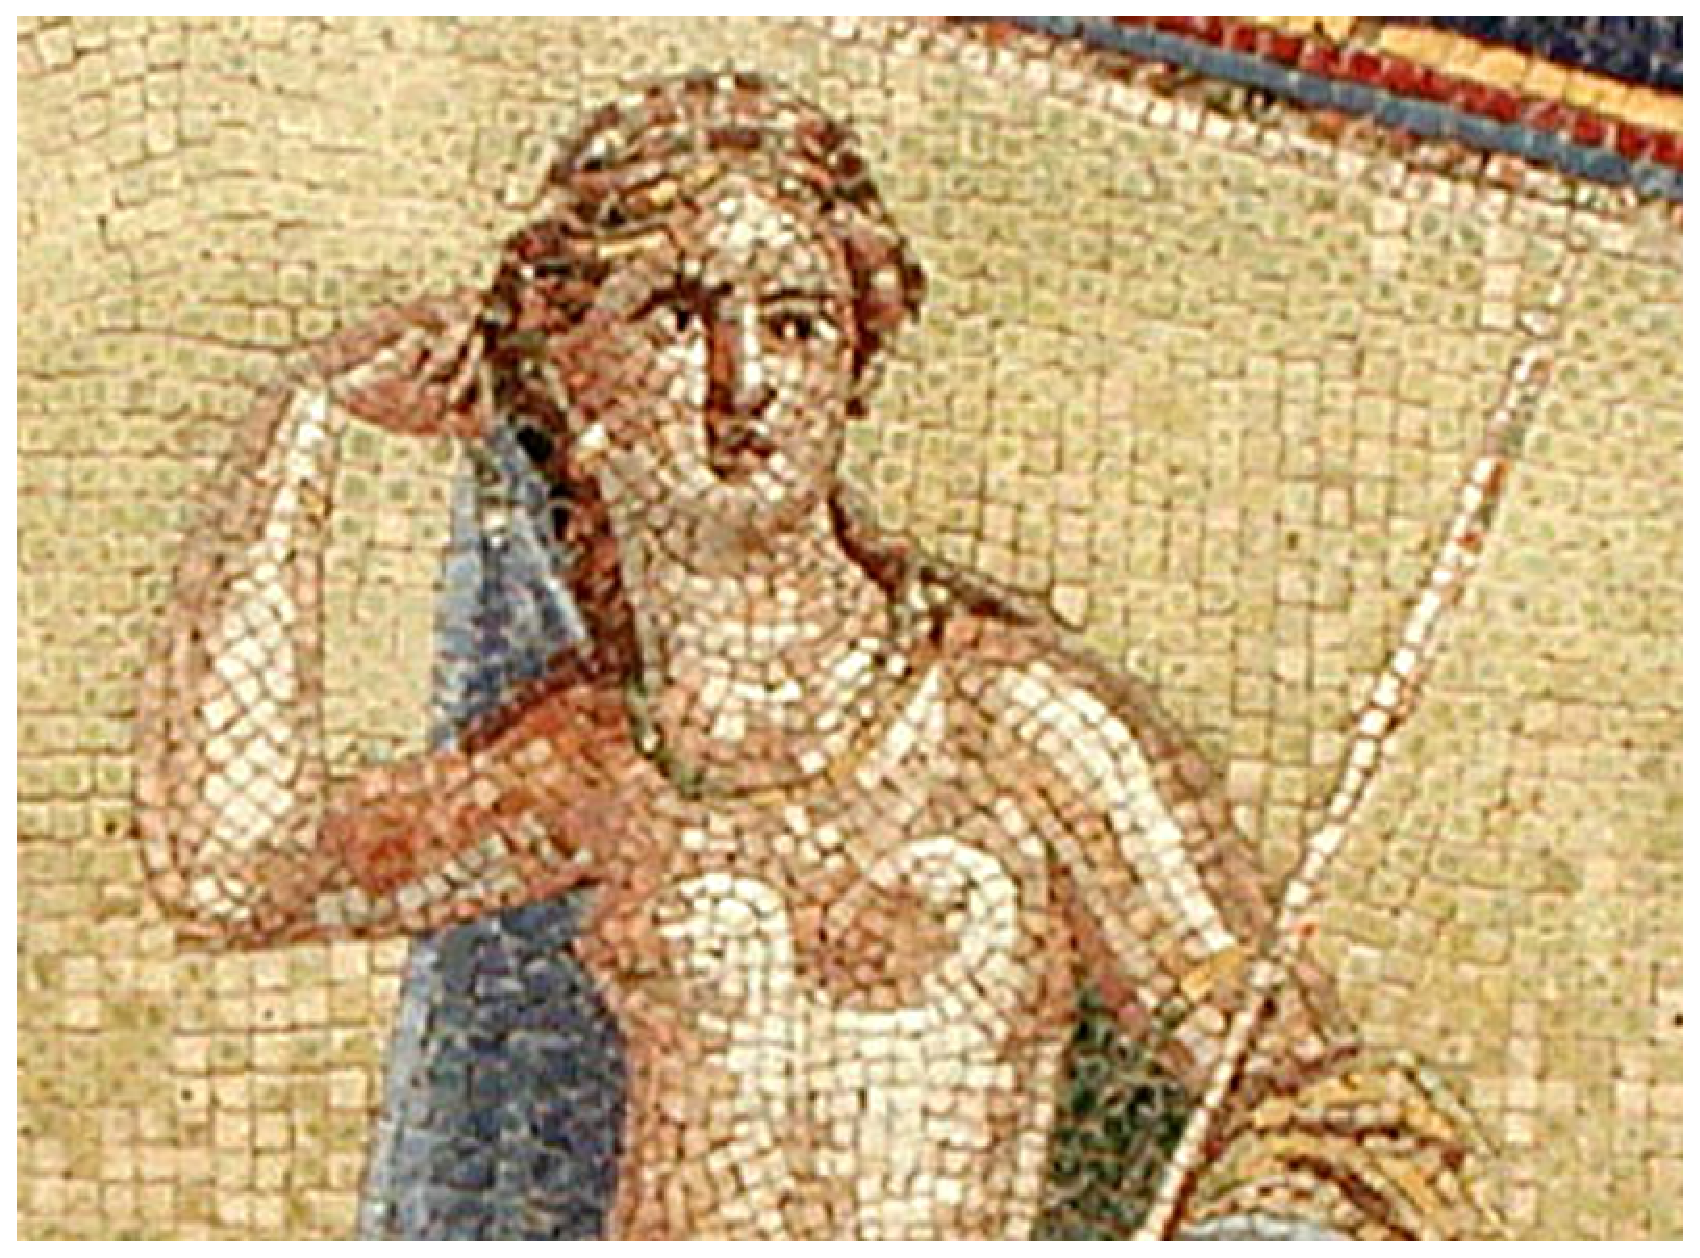
\includegraphics[width=7cm]{mosaique}
  \caption{D�tail d'une mosa�que
    � Herculaneum, repr�sentant Amphitrite.}
\label{fig:mosaique}
\end{figure}

Usuellement, les   images   num�riques sont fournies   sur  un support
r�gulier, avec  un  espace $I'$ correspondant �   trois canaux (Rouge,
Vert, Bleu, not� RVB) o�  chaque canal contient  une intensit� sur  un
intervalle $[0,255]$ (voir figure \ref{fig:lenna}).

\begin{figure}[h]
  \centering
  \includegraphics[width=12cm]{lenna_complet}
\caption{Repr�sentation  d'une image  sur un support discret
    r�gulier.}
\label{fig:lenna}
\end{figure}




\section{Espace discret et connexit�}

\subsection{Pavages et maillages}


Par la suite, nous appelons {\it espace  discret} un pavage du plan en
dimension deux, ou plus g�n�ralement de l'espace en dimension trois ou
plus.  Nous appelons aussi {\it point discret} le centre de gravit� de
chaque  cellule dans le  pavage consid�r�.    Dans  ce qui suit,  nous
repr�sentons graphiquement l'espace discret, soit  par le pavage, soit
par le maillage issu de ce  pavage. Le maillage correspond � un graphe
dont  les  sommets sont les  points  discrets et   dont les ar{\^e}tes
repr�sentent les  adjacences  entre cellules, �l�ments  du pavage.  La
figure   \ref{fig:pavage_maillage}   pr�sente  les  trois   pavages et
maillages possibles en dimension deux. 


\begin{figure}[htbp]
  \begin{center}
    % 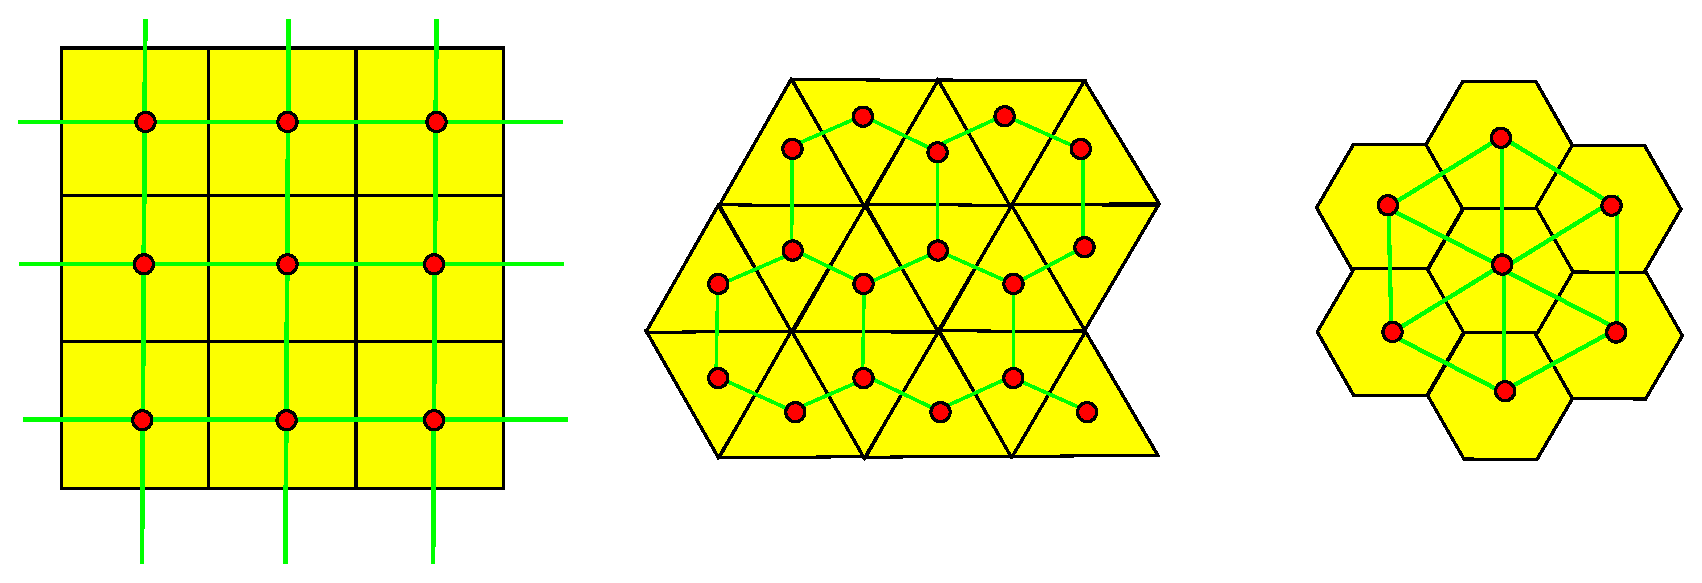
\includegraphics[width=12cm]{pavage_maillage}
    \includegraphics[width=12cm]{pavage_maillage2} 
  \end{center}
  \caption{\label{fig:pavage_maillage}Pavages (et maillages) r�guliers
    en dimension deux par  cellules carr�es, triangulaires et  hexagonales.}
\end{figure}
  
Certaines partitions de l'espace peuvent �tre �tudi�es, donnant lieu �
des pavages qui ne sont  pas forc�ment r�guliers \cite{Grunbaum}.  Par
ailleurs d'autres repr�sentations de  l'espace sont parfois utilis�es.
Par  exemple  en  dimension  trois,  les  repr�sentations  BCC  et FCC
{\it(body-centered    cubic,  face-centered      cubic)},  issues   de
l'organisation des cristaux, poss�dent des propri�t�s particuli�res de
sym�trie et de densit�, qui  peuvent �tre exploit�es pour le codage et
le traitement d'images.


De par la physique des capteurs, le pavage par des  carr�s est le plus
usuel,   m�me si,   comme  nous    le  verrons   par la  suite,    ses
caract�ristiques  topologiques ne sont pas  toujours les plus simples.
En dimension sup�rieure � deux,  les seuls espaces discrets  r�guliers
sont ceux  engendr�s  par des  cubes  multi dimensionnels.  Les points
discrets     associ�s {\`a}  ces  espaces sont    donc  des points  de
$\mathbb{Z}^d$ pour la dimension $d$.

En terme de codage,  l'espace discret engendr�  par le pavage avec des
carr�s  offre   une repr�sentation   matricielle  directe~:  une image
correspondra � une  partie de $\mathbb{Z}^2$.  Dans le cas des pavages
par des  triangles ou par   des hexagones, un  codage particulier  est
n�cessaire, mais nous     pouvons   toujours consid�rer  la     grille
$\mathbb{Z}^2$  (voir  figure~\ref{fig:codage}).    L'int�r�t    d'une
repr�sentation matricielle est  qu'elle permet un adressage direct des
�l�ments (un  couple de coordonn�es pour  chaque point  discret) ainsi
qu'une extraction rapide des points discrets voisins.

\begin{figure}[ht]
  \centering
  \includegraphics[width=12cm]{voisins} 
\caption{\label{fig:codage}Repr�sentation et codage  des  pavages  r�guliers 2D   sous
    forme matricielle.}
\end{figure}


Dans le chapitre \ref{chap:IA}, nous nous  int�ressons � une classe de
pavages   et de  maillages   un  peu  diff�rente~: les   \emph{grilles
  isoth�tiques irr�guli�res}.   Cette classe consiste �  consid�rer un
pavage avec des  carr�s   et � rel�cher les  contraintes  sur  la taille  des
cellules,  ainsi que sur  la  position de leur  centre.  Supposons une
cellule d�finie comme un rectangle donn� par un centre $p\in\R^2$, une
largeur $l_x$ et une hauteur $l_y$  ($l_x,l_y\in\R$).  En fonction des
contraintes  que nous imposons  sur $p$, $l_x$  et $l_y$, nous pouvons
d�finir des \emph{pavages isoth�tiques} comme  un ensemble de cellules
tel que l'intersection de tout couple de  cellules est soit vide, soit
de  dimension inf�rieure ou �gale �  1. Notons que ces pavages peuvent
ne  pas  paver  le plan  mais   dans  nos applications,   ils paveront
g�n�ralement un domaine rectangulaire (voir chapitre \ref{chap:IA}).

Par  exemple   (voir  figure    \ref{fig:isoth}),  si  $p\in\Z^2$   et
$l_x=l_y=1$,   nous   d�finissons  le   pavage   r�gulier  par   carr�
($\mathbb{D}$).  En consid�rant  maintenant des rectangles de  taille
uniforme $l_x=\lambda$  et $l_y=\mu$  ($\lambda,\mu\in\R$)  avec pour
centres  $p=(\lambda   i,\mu    j)$   ($(i,j)\in\Z^2$), nous   pouvons
caract�riser les grilles  avec �longation, tr�s utilis�es  en imagerie
m�dicale  car de nombreux   appareils d'acquisition n'ont pas  la m�me
r�solution suivant toutes les dimensions.

\begin{figure}[h]
  \centering
  \includegraphics[width=14cm]{schemabis}
  \caption{Structuration possible    de  quelques grilles isoth�tiques
    irr�guli�res.}
  \label{fig:isoth}
\end{figure}


De mani�re similaire, si nous consid�rons non plus des contraintes sur
la forme des cellules isoth�tiques ind�pendemment les unes des autres,
mais  des  contraintes globales  comme  des r�gles de subdivision d'un
rectangle initial (par  des droites horizontales ou  verticales), nous
pouvons caract�riser des  pavages issus de grilles hi�rarchiques comme
le \emph{quadtree} ($\mathbb{Q}$) \cite{samet90}. Si nous consid�rons
des regroupements/fusions de cellules issues d'un pavage r�gulier, nous
pouvons d�finir les  grilles adaptatives ($\mathbb{A}$) (voir par
exemple \cite{havran} pour une �tude de ces diff�rentes grilles dans
le cas de l'acc�l�ration d'une lancer de rayons en synth�se d'images).

L'int�r�t  d'avoir  une �criture   unifi�e, sous  le  nom  de  grilles
isoth�tiques irr�guli�res, de ces pavages est  de pourvoir d�river des
d�finitions d'objets ou des algorithmes g�n�riques transversaux � tous
ces  mod�les.  Le chapitre \ref{chap:IA}  pr�sente quelques-uns de ces
outils.


\subsection{Voisinages}
\label{sec:voisinages}

Sur un  espace  discret,   nous  introduisons  des notions  de    {\it
  voisinage} permettant de construire  des graphes d'adjacence ou, dit
plus simplement, de d�tecter  si deux pixels sont  voisins ou non.  Si
nous  consid�rons l'espace discret   2D  g�n�r� par des carr�s,   nous
d�finissons le {\it $4-$voisinage} comme �tant la relation d'adjacence
par ar{\^e}tes dans la partition de l'espace et le {\it $8-$voisinage}
comme �tant la  relation d'adjacence par  ar{\^e}tes et sommets.  Plus
formellement, deux points $A$ et $B$ de $\mathbb{Z}^2$, de coordonn�es
respectives ($x_A$,  $x_B$) et ($y_A$,   $y_B$) sont {\it $4-$voisins}
(ou {\it $4-$adjacents}) si :
\begin{displaymath}
  |x_A - x_B| + |y_A - y_B| =1\,.
\end{displaymath}

De la m{\^e}me mani�re, deux points $A$ et $B$  de $\mathbb{Z}^2$ sont {\it
  $8-$voisins}  (ou {\it $8-$adjacents}) si :
\begin{displaymath}
  max(|x_A-x_B|,|y_A-y_B|)=1\,.
\end{displaymath}


En dimension trois, nous pouvons introduire  les notions de {\it $6-$,
  $18-$} ou {\it   $26-$voisinage} en consid�rant les   adjacences par
faces, ar{\^e}tes et sommets (voir figure \ref{fig:adjacences3D}). Ces
adjacences      sont   donn�es  formellement       dans    le  tableau
\ref{tab:caract_adjacence}.


\begin{table}[!h]
  \begin{center}
    \begin{tabular}{|l|r|}
      \hline
      adjacence & caract�risation \\
      \hline
      $6$ &  $|x_A - x_B| + |y_A - y_B| + |z_A - z_B|=1$\\
      $18$ & $A$ et $B$ sont 26-voisins et $|x_A - x_B| + |y_A - y_B| + 
      |z_A - z_B| \leq 2$\\
      $26$ & $max(|x_A-x_B|,|y_A-y_B|,|z_A - z_B|)=1$\\
      \hline
    \end{tabular}
 \caption{Caract�risation des adjacences en dimension trois.}
    \label{tab:caract_adjacence}
  \end{center}
\end{table}

Dans ce qui suit, on parle d'$\alpha$-adjacence, pour $\alpha\in\{4,8,6,18,26\}$.

\begin{figure}[htbp]
\begin{center}
  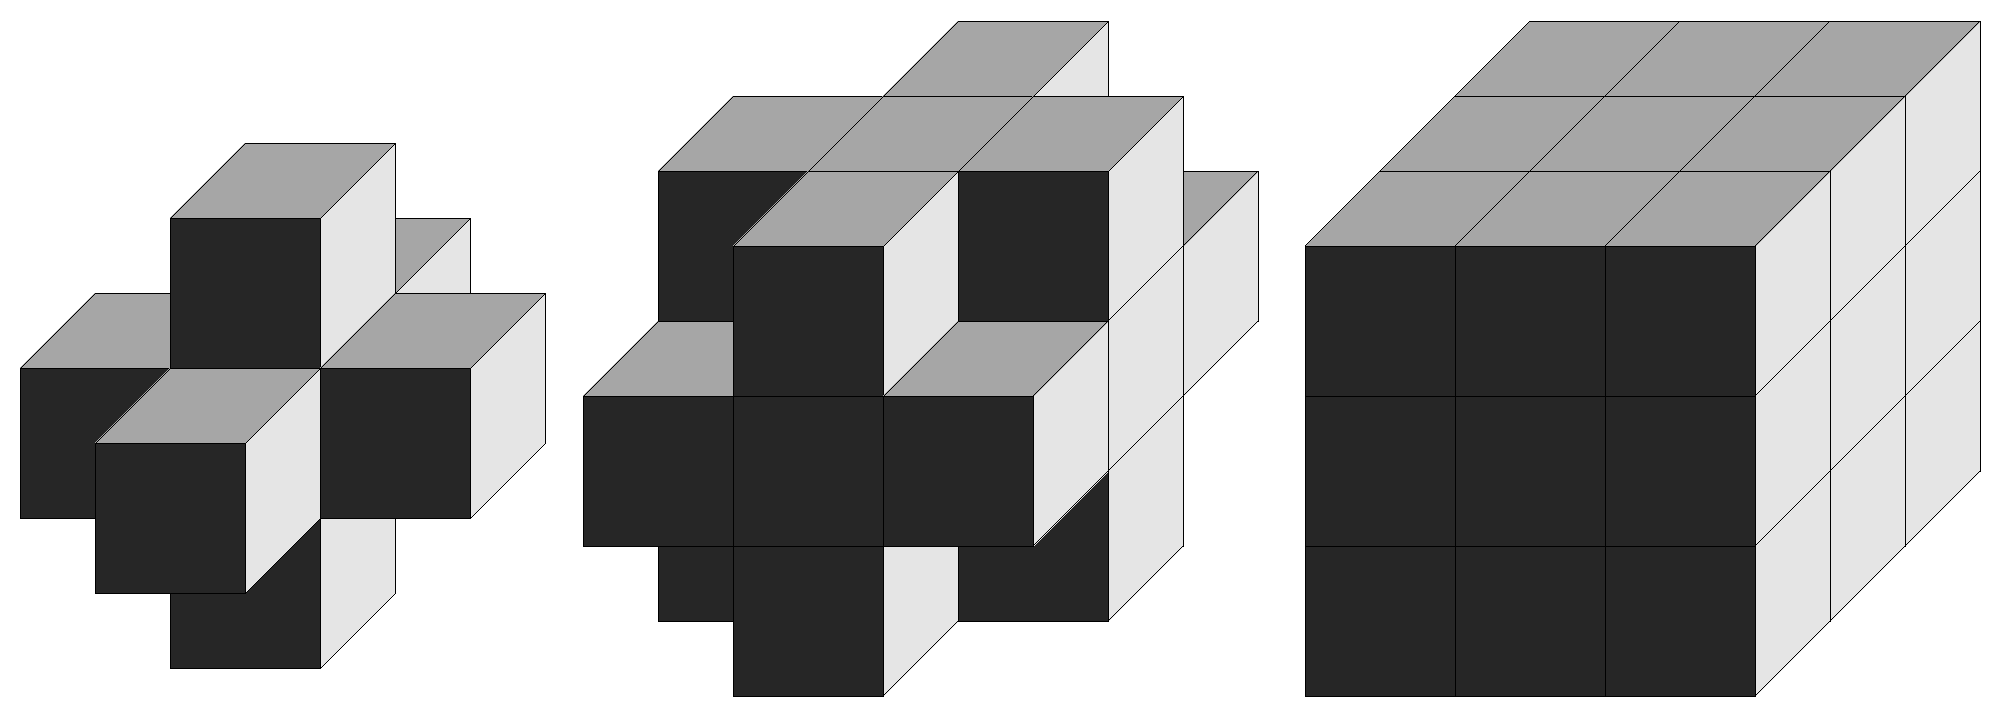
\includegraphics[width=8cm]{connexite}  
\end{center}
\caption{\label{fig:adjacences3D}En 3D, diff�rents voisinages du cube central avec le pavage r�gulier.}
\end{figure}

Une �criture   unifi�e  de   ces  diff�rentes  relations   d'adjacence
s'exprime sous la forme   de {\it $(r)-$voisinage},  g�n�ralisable aux
dimensions  sup�rieures :  deux   points de $\mathbb{Z}^d$   sont {\it
  $(r)-$voisins} si  chaque coordonn�e diff�re au plus  de  1 et qu'au
moins  $r$ coordonn�es sont �gales.   Alors, les connexit�s  4 et 8 en
dimension 2 sont not�es respectivement  $(1)-$ et $(0)-$voisinage.  De
m�me, les  connexit�s  6, 18  et 26   en  3D s'�crivent respectivement
$(2)$, $(1)$ et $(0)$ (voir table  \ref{tab:vois} pour une comparaison
des diff�rentes notations).  Une mani�re plus  simple de consid�rer le
$(r)-$voisinage est de regarder la dimension de l'intersection de deux
pixels~: deux pixels  (carr�s    unit�s   ferm�s) $A$  et   $B$   sont
$(1)-$voisins  si l'intersection de  $A$ et $B$ contient un �l�ment de
dimension 1 (un segment en 2D).  De m�me, $A$ et  $B$ sont pixels sont
$(0)-$voisins si  leur intersection contient des �l�ments de dimension
sup�rieure � $0$ (un point ou un segment en 2D).

\begin{table}[htbp]
  \begin{center}
    \begin{tabular}{|c|c|c|}
      \hline
    $(r)-$voisinage &    $\alpha-$voisinage\\
      
     % $n-1$ &  $2D$ & $3D$ & $nD$\\
    \hline
    $0$   & $3^d -1$ \\
    \ldots  & \ldots\\
    $d-r$ & $\sum_{i=d-r}^{d-1} \frac{d!}{i!(d-i)!}2^{d-i}$ \\
    \ldots&  \ldots\\
    $d-2$ &   $2d^2$ \\
    $d-1$ &     $2d$ \\
    \hline
    \end{tabular}
    \caption{Lien entre les notations de voisinage pour un pavage  par hypercubes.}
    \label{tab:vois}
  \end{center}
\end{table}


Cette illustration g�om�trique de la $(r)-$adjacence est g�n�ralisable
aux dimensions  sup�rieures de la grille discr�te,  mais aussi  au cas
des grilles  isoth�tiques irr�guli�res (voir figure \ref{fig:adj_iso}).  

\begin{figure}[ht]
  \centering
  \includegraphics[width=8cm]{adjacence_isoth}
  \caption{A gauche, $A$ et $B$ sont $(1)-$ et $(0)-$adjacents, �
    droite, $A$ et $B$ sont $(0)-$adjacents mais pas $(1)-$adjacents.}
  \label{fig:adj_iso}
\end{figure}


% \begin{table}[htbp]
%   \begin{center}
%     \begin{tabular}{|c|c|c|c|}
%       \hline
%       $O(r)$-voisinage &       \multicolumn{3}{|c|}{$\alpha-$voisinage}\\ \cline{2-4}
      
%        &  $2D$ & $3D$ & $nD$\\
%        \hline
%        1 & 4 & 6 & $2n$\\
%        2 & 8 & 18 & $2n^2$\\
%        3 & . & 26 & \ldots\\
%        \ldots& . &. & \ldots\\
%        $r$ & . & . & $\sum_{i=n-r}^{n-1} \frac{n!}{i!(n-i)!}2^{n-i} $\\
%       \ldots& . &. & \ldots\\
%       $n$ & . & . & $3^n -1$\\
%       \hline
%     \end{tabular}
%     \caption{Liens entre notations de voisinage pour un pavage  par hypercubes.}
%     \label{tab:vois}
%   \end{center}
% \end{table}



\section{Objets, courbes, surfaces}

\label{chap:partie3}           

\subsection{D�finitions classiques}
\label{sec:defin-class}

Dans l'espace discret, nous d�crivons les objets �l�mentaires utilis�s
par la suite.  Nous  notons  $r\in\{0,1,2\}$ la  relation  d'adjacence
consid�r�e   sur la grille  discr�te $\Z^d$   pour $d\in\{2,3\}$.  Ces
relations d'adjacence nous permettent tout  d'abord de d�finir un {\it
  $(r)$-chemin} sur l'espace discret~:


\index{$(r)-$chemin}
\begin{definition}[$(r)-$chemin]{Soit    un ensemble  $X$ de points
    discrets et  une relation de $(r)-$adjacence. Un $(r)-$chemin
    (dans $X$) joignant deux points $A$ et $B$ de $X$ est une s�quence
    $\pi = (A_0, \ldots, A_n)$ de pixels de $X$ telle que $A_0 =
    A, A_n =   B$ et  $A_i$  est
    $(r)$-voisin de $A_{i-1}$ pour tout $i = 1, \ldots n$.}
%
%  $X$ est  un
%    $(r)-$chemin,  not�  $\pi$, si   tous   les �l�ments de $X$
%    poss�dent au moins un $(r)$-voisin dans $X$.}
\end{definition}



Nous pouvons  d�finir de la m{\^e}me mani�re  un objet  dans un espace
discret muni d'une relation d'adjacence.

\index{$(r)-$objet}
\begin{definition}[$(r)-$objet]{  Soit un  ensemble $X$  de  points
    discrets   et  une relation  de   $(r)-$adjacence.  $X$ est  un
    $(r)-$objet si pour tout couple $A$ et $B$ de $X$, il existe un
    $(r)-$chemin dans $X$.}
\end{definition}

En  d'autres termes, un $(r)-$objet est   une composante connexe de
points discrets au sens de la $(r)-$adjacence.\index{composante connexe}
La  notion  de $(r)-$chemin  d�crite  ci-dessus est  tr�s g�n�rale.
Nous restreignons cette  notion pour pouvoir introduire des propri�t�s
topologiques plus complexes.

\index{$(r)$-courbe ferm�e}
\begin{definition}[$(r)-$courbe      ferm�e]{Soit       $\pi$    un
    $(r)-$chemin. $\pi$ est une  $(r)-$courbe ferm�e si tous les
    �l�ments de $\pi$ ont exactement deux points $(r)-$voisins dans
    $\pi$.}
\end{definition}
Finalement,  si nous  d�connectons  une  $(r)-$courbe  ferm�e, nous
d�finissons tout simplement une $(r)-$courbe.

\index{$(r)-$courbe}
\begin{definition}[$(r)-$courbe]{ Soit $\pi$ un $(r)-$chemin. $\pi$
    est une $(r)-$courbe si, pour tous les �l�ments $\{A_i\}$ de $\pi$, $A_i$
    a exactement deux points $(r)-$voisins, sauf $A_0$ et $A_n$ qui
    n'en  ont  qu'un ($A_0$  et  $A_n$  sont alors  les  extr�mit�s de
    la courbe).}
\end{definition}

% Si le $(r)-$arc est ferm� on parle alors de $(r)-$courbe ferm�e.


% \begin{definition}
% Soit $d \in \{2,3\}$ et soit $(r) \in \{4,8, 6,18,16\}$ une
% relation d'adjacence sur $\Z^d$.\\
% {\bf 1)} Une $(r)-$courbe ferm�e simple $X$ dans $\Z^d$ est une
% partie de $\Z^d$ telle que tout point de $X$ soit $(r)-$adjacent
% � exactement deux autres points de $X$ \\
% {\bf 2)} Une $(r)-$courbe ferm�e simple param�tr�e est un
% $(r)-$chemin ferm� $\pi = (A_0,\ldots,A_n)$ telle que
% $A_i$ soit $(r)-$adjacent � $A_j$ si et seulement si $j\% n \in \{(i-1)\% n, (i+1)\% n\}$.
% \end{definition}



L'introduction des courbes  l�ve des probl�mes topologiques. En effet,
une propri�t� {\it souhaitable}  sur une $(r)-$courbe ferm�e dans
$\Z^2$  serait que l'on puisse d�finir un int�rieur et un ext�rieur � cette courbe.  
Ces d�finitions
sont li�es {\`a} la notion de  propri�t� de \OldName{Jordan} en g�om�trie
diff�rentielle classique.

\begin{figure}[!h]
  \centering
  \includegraphics[width=12cm]{remplissage} 
  \caption{Illustration d'un   remplissage d'objet �  partir du  pixel
    noir  en  $(1)-$connexti�  (\emph{gauche}) et  en  $(0)-$connexit�
    (\emph{droite}). Les fl�ches illustrent  un exemple de propagation
    selon la connexit� consid�r�e.}
\label{fig:remplissage}
\end{figure}


Pour illustrer  cette   notion, prenons l'exemple  d'un processus  de
remplissage tr�s simple~: �tant  donn� un  pixel \emph{source}  (pixel
noir dans  la   figure \ref{fig:remplissage}),  le  remplissage  d'une
r�gion se fait en  coloriant tous les  voisins selon une connexit� $r$
de $(0)$    ou   $(1)$.  Sur   la   courbe   donn�e  dans  la   figure
\ref{fig:remplissage}, nous voyons   que, parmi  les deux   connexit�s
possibles  du  remplissage,  seul   le  remplissage en $(1)-$connexit�
remplit  effectivement   la  courbe    discr�te sans d�border.   En  utilisant    la
$(0)-$connexit�, tout l'espace   discret est rempli, ce qui  peut �tre
critique   dans    certaines   applications.      La    propri�t�   de
\OldName{Jordan}    permet    de    formaliser     cette   notion   de
\emph{perm�abilit�} d'un contour.   L'�nonc� de cette  propri�t� ainsi
que les techniques permettant la caract�risation des objets  discrets
la  v�rifiant  est un probl�me   tr�s classique en g�om�trie discr�te.
D'une  mani�re g�n�rale, deux grandes  approches sont consid�r�es dans
ces formalisations~:   la  premi�re consiste �    d�finir les  contours
d'objets discrets comme des s�quences de  points discrets.  La seconde
se  base sur  une d�composition  cellulaire de  la grille (voir figure
\ref{fig:cellules})    et d�finit le    contour  d'un objet comme  les
�l�ments de dimension inf�rieure (� la dimension de l'espace) s�parant
les   pixels ou  les voxels  de   l'objet,  de ceux  du compl�mentaire
\cite[chap. 3]{dcoeurjo_hermes}.


\begin{figure}[htbp]
\begin{center}
%  \includegraphics[width=3cm]{cellulaire}
  \includegraphics[width=\textwidth]{elements}
\end{center}
\caption{\label{fig:cellules}D�composition d'un pixel et d'un voxel en cellules
    de dimensions inf�rieures.}
\end{figure}

% La  figure \ref{fig:remplissage} sugg�re   de d�finir le contour comme
% une  $(r)-$courbes  dans l'espace  discret.  Cependant,  la  figure
% \ref{fig:topoerreur}   illustre le paradoxe   de connexit� dans le cas
% d'un pavage  par carr�s du  plan.  Sur la  partie gauche de la figure,
% les  pixels noirs  forment une $8-$courbe  ferm�e  mais  il  existe un
% $8-$chemin  entre  l'ext�rieur et le  pixel   blanc int�rieur {\`a} la
% courbe.  La propri�t� de s�parabilit� n'est donc pas v�rifi�e.  Sur la
% partie droite de la figure \ref{fig:topoerreur}, nous observons le cas
% o{\`u}  une $4-$connexit� est utilis�e  pour  les pixels blancs et les
% pixels noirs, dans ce  cas il n'existe  pas de $4-$chemin joignant les
% pixels blancs au pixel central, et les pixels noirs  ne forment pas un
% $4-$chemin.  Il y a  donc un choix  crucial � faire entre la connexit�
% de l'objet et la connexit� du fond.



% \begin{figure}[htbp] 
% \begin{center}
%   \includegraphics[width=8cm]{topoerreur}
% \end{center}
% \caption{Paradoxe de connexit� pour un maillage par carr�s, les ar�tes
%   de   ces     graphes repr�sentant    les   diff�rentes    connexit�s
%   choisies.\label{fig:topoerreur}}
% \end{figure}

\subsection{D�finitions pour les grilles isoth�tiques irr�guli�res}
\label{sec:definitions-irr}

Dans  le cas des   grilles isoth�tiques irr�guli�res, les  d�finitions
pr�c�dentes   sont   tout �  fait  valident  pour   la    $(0)-$ et  la
$(1)-$adjacences d�finies sur ces cellules.  Nous avons donc de mani�re
triviale, des $(r)-$objets ou encore des $(r)-$courbes ferm�es dans ces
espaces (voir figure \ref{fig:courbe_isoth}).


\begin{figure}[htbp]
\begin{center}
%  \includegraphics[width=3cm]{cellulaire}
  
\includegraphics[width=10cm]{courbe_isoth}
\end{center}
\caption{\label{fig:courbe_isoth}Exemples d'objets topologiques sur
  une grille isoth�tique irr�guli�re~: \emph{(de gauche � droite)} un
  $(1)-$objet (mais non $(0)-$objet), une ($0)-$courbe et une $(0)-$courbe ferm�e.}
\end{figure} 

Pour  retrouver   une  d�finition de contour   sur   ces espaces, nous
consid�rons un pavage  de cellules �tiquet�es avec un label  ``objet''
ou  ``fond''.   Ensuite, nous pouvons   nous  baser sur  la notion  de
surface    de   \aut{Jordan}   sur    un    graphe    bicolore orient�
\cite{Herman98b}~: les sommets  du graphe sont les cellules  colori�es
``objet'' ou ``fond'', et les  ar�tes sont donn�es explicitement par le
graphe d'adjacence des cellules pour une certaines connexit�s.



\section{El�ments g�om�triques}


Sur les pavages r�guliers, nous avons  pour l'instant caract�ris� les
objets discrets selon  leurs propri�t�s  topologiques, ou selon le processus de 
discr�tisation  d'un objet r�el dont ils sont issus.

Nous pouvons  cependant  d�finir un  paradigme g�om�trique  de mani�re
intrins�que � la  grille   discr�te.    Ce   paradigme regroupe    des
d�finitions d'objets   g�om�triques �l�mentaires     (points, droites,
plans, segments, cercles,  etc.),  des propri�t�s entre ces   objets,
ainsi que des algorithmes permettant de les manipuler efficacement.

\subsection{Objets discrets~: droites, plans, cercles, etc.}
\label{sec:objets-discrets}

Dans le paradigme de la g�om�trie  discr�te,  il est n�cessaire de  d�finir  des
objets  g�om�triques    de    base.   G�n�ralement,    deux   approches
compl�mentaires sont possibles  ; nous les illustrons avec la  d�finition
d'une droite discr�te~:
\begin{itemize}
\item d�finition par discr�tisation~: on d�finit la droite discr�te
  comme �tant le  r�sultat  d'une   discr�tisation, selon  un  certain
  processus, d'une droite r�elle~;
\item d�finition  intrins�que~:  on d�finit  la droite  discr�te comme
  �tant l'objet g�om�trique  qui     valide la version  discr�te    de
  certaines propri�t�s g�om�triques que poss�de la droite r�elle.
\end{itemize}

Souvent  ces deux processus se  rejoignent et d�crivent le m�me objet.
Reprenons la d�finition  par  discr�tisation, s'il est �vident que  la
figure \ref{fig:vialard_droites}.c   ne  peut pas �tre  un  morceau de
droite discr�te,  le  fait que la   courbe \ref{fig:vialard_droites}.b
n'en  soit pas un non plus  illustre le fait  que ces objets poss�dent
une  structure intrins�que.  Plus  pr�cis�ment, la droite  discr�te de
pente  rationnelle,   tout comme  le  plan discret   dans une certaine
mesure, poss�de des structures de r�gularit� et de p�riodicit� faisant
le  lien  entre ces     objets   et des r�sultats   fondamentaux    en
arithm�tique,    th�orie des nombres,  th�orie    des mots, etc.   Une
bibliographie     tr�s    dense        existe    sur     ces �l�ments,
\cite{citeulike_611268,dcoeurjo_planarity}     pr�sentent    un nombre
cons�quent de r�f�rences.

\begin{figure}[htbp]
  \begin{center}
    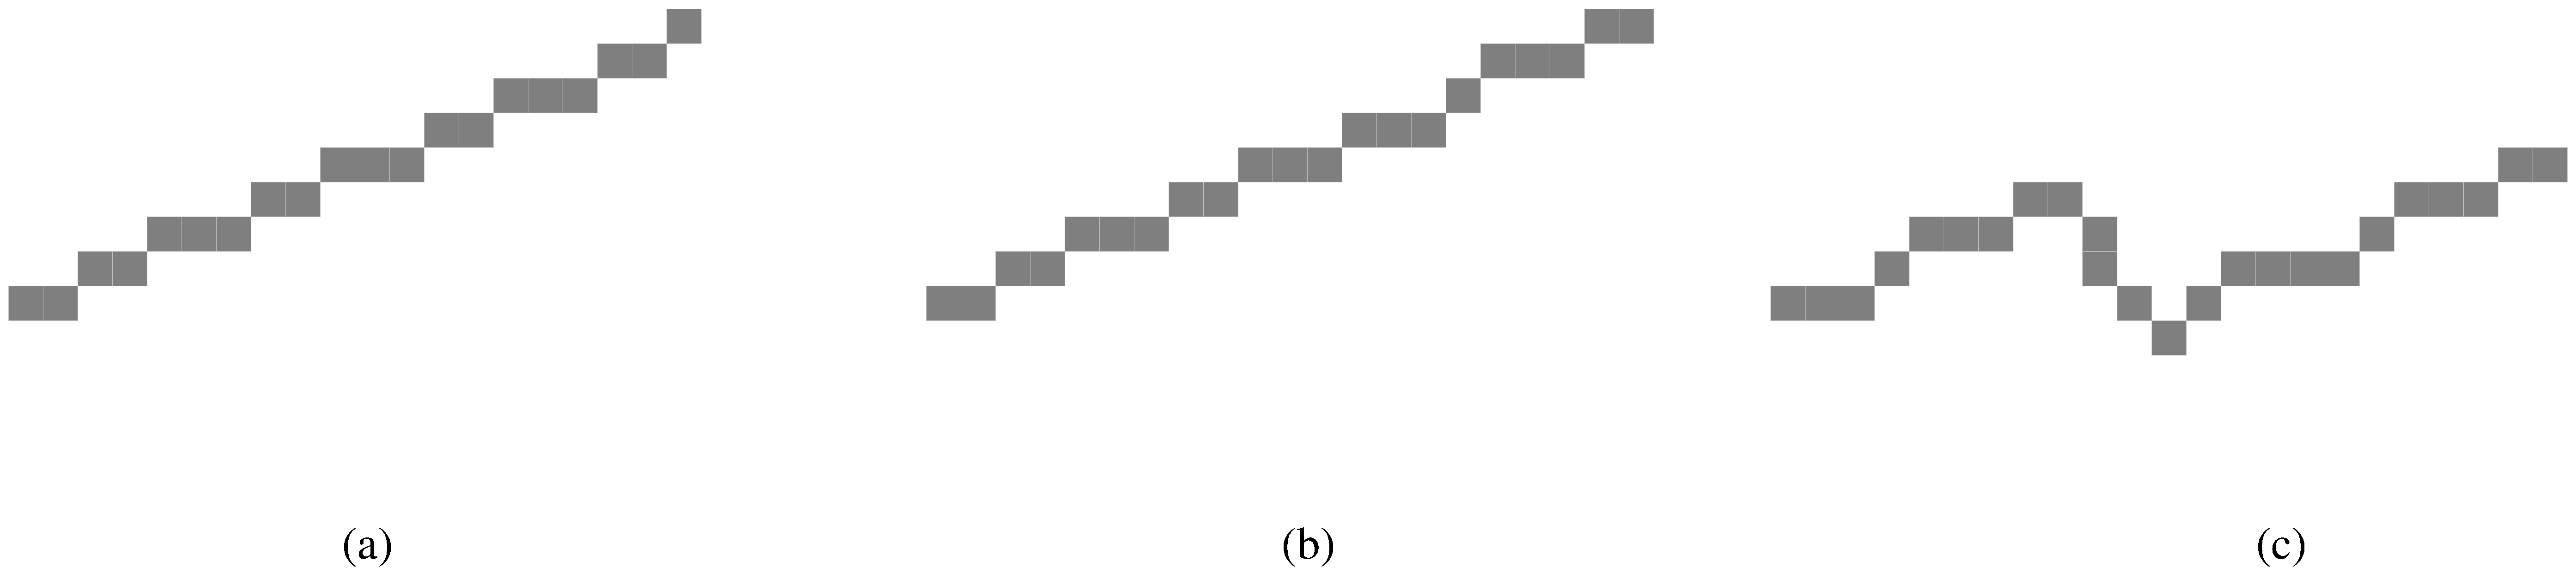
\includegraphics[width=12cm]{droite_vialard}
\end{center}
\caption{Seule la courbe $(a)$ est un segment discret selon
      les d�finitions usuelles des droites discr�tes.\label{fig:vialard_droites}}
\end{figure}

En utilisant la  droite discr�te dans  notre  mod�le g�om�trique, nous
pouvons d'ores et d�j� nous rendre compte que les axiomes g�om�triques
d'\OldName{Euclide}  seront �  revoir.   En effet,  l'intersection, en
termes de  points   et donc de  pixels   communs,  entre deux  droites
discr�tes non parall�les peut �tre compos�e d'un point, d'aucun point,
d'un ensemble connexe de points ou encore d'un ensemble non connexe de
points.  De m�me, deux  droites discr�tes parall�les  peuvent partager
une infinit� de  points sans �tre confondues.   Il faut  donc repenser
les      propri�t�s       d'intersection     et       de  parall�lisme
\cite{Vee99,Vee02,citeulike_613266}.

Ce probl�me, pos� par les axiomes d'\aut{Euclide}, illustre parfaitement
la probl�matique de la g�om�trie discr�te~: le lien avec l'objet ou le
concept   continu  sous-jacent est �  consid�rer   avec   beaucoup  de
pr�cautions.  Parfois  nous aurons des  constructions ou des r�sultats
intrins�ques au mod�le discret    sans  aucun lien avec  le   continu,
parfois nous   d�finirons     nos objets discrets      comme �tant des
approximations les plus pr�cises possibles d'objets continus.

Dans  le chapitre  \ref{chap:IA}  nous revenons   sur  les mod�les  de
discr�tisation, et sur les liens discrets/continus.

�tant donn�e  une d�finition d'un  objet  fondamental comme  la droite
discr�te, une  question   r�currente est d'obtenir   un  algorithme de
reconnaissance~: consid�rons un ensemble de  pixels (pour l'exemple de
la droite discr�te), un algorithme de reconnaissance doit d�cider s'il
existe une droite discr�te contenant l'ensemble des pixels consid�r�.
De plus, comme la  d�finition de la droite  discr�te est param�tr�e par
des quantit�s   (pente,   ordonn�e �  l'origine), nous    attendons de
l'algorithme qu'il nous   retourne  aussi un param�trage valide   pour
l'ensemble  (dans   le cas    o�  ce   dernier  est bien  un
sous-ensemble de  droite  discr�te). Bien  s�r, ces   techniques  vont
exploiter   les  propri�t�s internes  des   objets � reconna�tre  afin
d'obtenir                des            algorithmes            rapides
\cite{citeulike_611268,dcoeurjo_planarity}. Le chapitre \ref{chap:ILP}
pr�sente une analyse th�orique  et algorithmique pour certains de  ces
objets.

Par d�finition des  objets  fondamentaux comme la droite  discr�te, un
param�trage valide  conduit g�n�ralement �  la d�finition d'une droite
r�elle associ�e avec  la  propri�t� que la discr�tisation  de celle-ci
corresponde exactement aux pixels de  la droite discr�te. Notons qu'il
existe une  infinit� de  droites r�elles se   discr�tisant dans une m�me
droite discr�te.



\subsection{Reconstruction  et poly�drisation r�versible d'objets discrets}
\label{sec:reconstr-et-poly}

Une probl�matique classique en g�om�trie discr�te consiste � convertir
une repr�sentation en extension   (un ensemble de pixels d'un  contour
discret) en une repr�sentation en compr�hension (courbe polygonale par
exemple). Bien �videmment,  ce changement   de repr�sentation se  doit
d'�tre r�versible dans le sens  o�, si l'on discr�tise l'objet  continu
(courbe polygonale), nous devons obtenir l'objet discret initial.

Dans  ce contexte, nous voyons bien  que  les objets fondamentaux vont
�tre des �l�ments de base  pour r�soudre ce probl�me. Nous utiliserons
en effet les  algorithmes  de reconnaissance  de  droite discr�te pour
d�composer un contour en segments. De m�me, nous pourrons utiliser les
algorithmes de reconnaissance  de plans discrets pour la facettisation
de surface d'objets discrets 3D (voir figure \ref{fig:reco}).

Si les probl�mes   paraissent simple, leurs   r�solutions ne sont  pas
triviales~:  m�me si la  d�finition des objets fondamentaux permet
d'assurer  la r�versibilit� le  long du  segment dans  le  cas 2D  par
exemple, le positionnement des sommets  n�cessite une analyse fine. En
dimension 3,     le placement des  sommets   et   des  ar�tes est
tout aussi difficile.


\begin{figure}[ht]
  \centering
  \subfigure[]{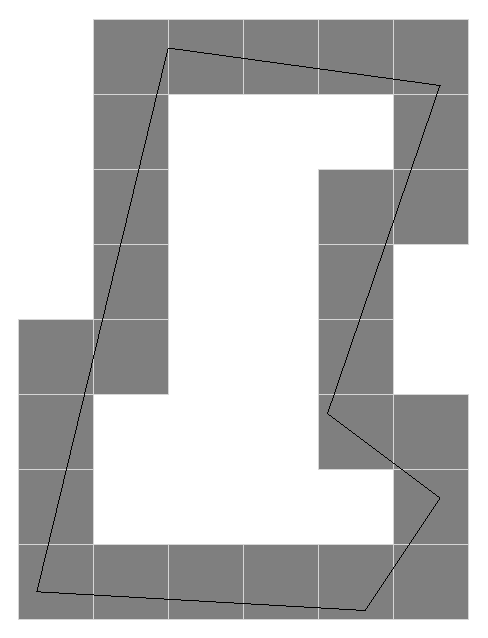
\includegraphics[width=3cm]{courbe_reco}}
  \subfigure[]{\includegraphics[width=4cm]{al}}
  \subfigure[]{\includegraphics[width=4cm]{al2}}
  \caption{Exemple de reconstruction r�versible en dimension 2 et 3.}
  \label{fig:reco}
\end{figure}

G�n�ralement, trois approches sont envisag�es  (illustr�es dans le cas
3D)~:
\begin{itemize}
\item approche \emph{Top-Down}~:   dans un premier  temps, nous  allons
  d�composer la surface en morceaux de plan maximaux selon un ensemble
  d'heuristiques  (voir  figure \ref{fig:reco}-$(b)$).   Ces  morceaux
  peuvent  donc d�finir une  infinit� de  facettes r�elles  et dans un
  second temps, nous cherchons � calculer  les facettes permettant  un
  \emph{recollement}            de         la                  surface
  \cite{journals/algorithmica/SivignonDC03,dcoeurjo_TFCV_graphe,sivignon_these,conf/dgci/SivignonDC05}~;
\item approche \emph{contrainte}~: la construction de la surface et la
  reconnaissance de plan discret se font  ici en parall�le. Pour cela,
  la reconnaissance est \emph{contrainte} par la surface polygonale en
  cours de construction   afin   d'obtenir la r�versibilit�   sur  les
  sommets  et les ar�tes, ainsi que  d'avoir la correction topologique
  \cite{dexet_these,dcoeurjo_mdexet_ISVC}.  Un inconv�nient est que la
  propagation des \emph{contraintes} a tendance � \emph{accumuler} les
  erreurs et  donc �  produire des poly�dres   tr�s irr�guli�res,
  avec des petites facettes~;
\item approche \emph{Bottom-Up}~: l'id�e est toujours de commencer par une
  d�composition   en  morceaux  de  plan,    mais nous  partons  d'une
  facettisation primaire �l�mentaire,   comme  celle   donn�e par   un
  algorithme                    de               \emph{Marching-Cubes}
  \cite{marching,Lachaud00a,citeulike_910101}, que    nous simplifions
  (fusion de facettes) en  int�grant l'information de  la segmentation
  en plans  discrets \cite{dcoeurjo_MCsimplDGCI06}.  Un �l�ment cl� de
  ce type de m�thodes et de maintenir, pour chaque op�ration locale de
  simplification de la surface, les propri�t�s  de r�versibilit� et de
  correction topologique   (figure  \ref{fig:reco}-$(c)$). La  section
  \ref{sec:reconstr-revers-en}  reviendra   plus  en d�tail sur  cette
  technique.
\end{itemize}

Notons que la qualit� de la  segmentation en morceaux de plan discret,
en terme  de nombre de morceaux,  influence grandement la  suite de la
reconstruction.  Cette   influence est   directe pour    les approches
\emph{Top-Down} et \emph{Bottom-Up}, mais elle  se retrouve aussi dans
les   approches  \emph{contraintes}.   Sur  ce   probl�me,  nous avons
cependant   d�montr�  un  r�sultat  th�orique  sur   le  fait que   la
segmentation en un nombre minimal de morceaux est NP-difficile dans le
cas  g�n�ral    \cite{dcoeurjo_NPhard}              (voir      section
\ref{sec:elem-de-compl} pour les notions li�es � la NP-compl�tude).

Dans  les  illustrations de la     figure \ref{fig:reco}, les   objets
discrets sont \emph{simples}~: nous avons  une courbe  (au sens de  la
section \ref{sec:defin-class})  en dimension 2   et une surface simple
(une seule composante connexe, sans trous, etc.)  en dimension 3. Dans
le cas de structures discr�tes  plus complexes avec des jonctions  par
exemple,  les probl�mes sont   plus   compliqu�s. 

Dans  le chapitre \ref{chap:IA},  nous revenons  sur  ces probl�mes de
reconstruction   en dimension   2 sur  des   formes  complexes,  et en
dimension 3.

Cette derni�re th�matique est �   rapprocher du domaine  du traitement
d'images, et plus particuli�rement  du traitement de documents, qu'est
la        \emph{vectorisation}          (voir        par       exemple
\cite{journals/pami/HilaireT06}  pour plus de r�f�rences).  Notons que
dans ce cadre applicatif, la r�versibilit� est une contrainte rarement
prise en compte. L'effort se porte sur des d�finitions statistiquement
robustes aux bruits plut�t qu'� des repr�sentations exactes.

\subsection{Distances discr�tes, transform�e en distance et axe m�dian}
\label{sec:dist-discr-transf}

Un autre  domaine d�taill�  dans  le chapitre  \ref{chap:AM} porte sur
l'analyse   volumique   d'objet   discrets  par  l'utilisation  de  la
transformation en distance. Cette transformation  consiste � �tiqueter
tous les points  d'un  objet discret  avec  leur distance  minimale au
compl�mentaire~; elle est   d'une grande utilit�  pour repr�senter les
objets discrets    par   des  unions de    boules,   d�finissant ainsi
\emph{l'axe m�dian} d'une forme discr�te (voir figure \ref{fig:am}).


\begin{figure}[ht]
  \centering
  \includegraphics[width=7cm]{am-cercles}
\caption{Illustration de  la repr�sentation d'une  forme par
    union   de  disques.  Les     centres des   disques   (pointill�s)
    repr�sentent    sch�matiquement        l'axe   m�dian     de    la
    forme.\label{fig:am}}
\end{figure}



Pour cela, nous devons sp�cifier la distance que l'on consid�re. Etant
donn�s  deux  points discrets $P$   et   $Q$, deux grandes  cat�gories
d'approches existent.    La premi�re consiste �  manipuler la distance
euclidienne      directement      en     consid�rant   le      vecteur
$\overrightarrow{PQ}$ ou encore le carr� de la distance, $d^2_e(P,Q)$.
La seconde  consiste �  approximer la   distance  euclidienne par  des
masques  locaux, donnant    lieu  aux  \emph{distances  de  chanfrein}
\cite{borgefors,Thiel_hdr}.   Ainsi,  en  consid�rant  une  famille de
d�placements �l�mentaires  pond�r�s, nous  pouvons construire un  plus
court chemin entre $P$ et $Q$ et estimer  la distance entre ces points
(voir figure \ref{fig:illustration-simple-distances}).

\begin{figure}[ht]
  \centering
  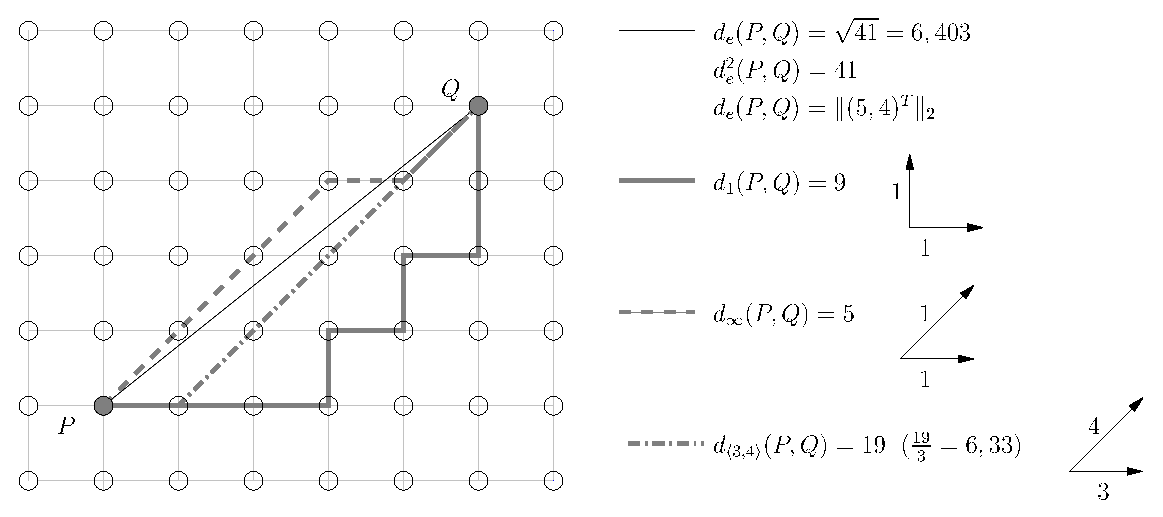
\includegraphics[width=12cm]{distances}
 \caption{Illustration de distances discr�tes entre deux points
    discrets. Les chemins correspondent � des plus courts chemins pour
    la distance consid�r�e (les d�placements �l�mentaires et leurs poids
    sont indiqu�s par les fl�ches).\label{fig:illustration-simple-distances}}
\end{figure}


G�n�ralement, les approches  fond�es sur une approximation en distance
de chanfrein �taient pr�f�r�es,  de par la simplicit�  des algorithmes
sous-jacents   (transformation    en  distance,  extraction   de l'axe
m�dian,\ldots).     N�anmoins,   nous  montrons   dans   le   chapitre
\ref{chap:AM} que des  algorithmes  tr�s  efficaces existent pour   la
m�trique euclidienne.


\section{�l�ments de complexit�}
\label{sec:elem-de-compl}

Dans   cette section,  nous   pr�sentons  rapidement  les  notions  de
complexit�  que nous utiliserons par la  suite. Plus pr�cis�ment, nous
reprenons  le sch�ma classique  de   preuve de NP-compl�tude que  nous
utilisons dans  le chapitre  \ref{chap:AM}.  Dans  ce  qui  suit, nous
consid�rons      un mod�le   g�n�rique  de   \emph{machine
  d�terministe �  acc�s al�atoire}, � processeur unique \cite{cormen}.
Une description  rapide  de ce mod�le affecte  un  co�t  unitaire pour
toutes   les  op�rations arithm�tiques, ainsi    que pour la comparaison de
nombres.   Pour quantifier     la complexit�  d'un    algorithme, nous
utilisons  g�n�ralement une analyse  au   pire cas, param�tr�e par  la
taille des donn�es  $n$ en entr�e  de l'algorithme.  Nous consid�rons
aussi les notations asymptotiques  de complexit� $O(g(n))$ d�finie  de
la mani�re suivante~:  si $f(n)=O(g(n))$, il  existe une constante $c$
et un  nombre $n_0$  tel que pour  tout  $n>n_0$, $f(n)< cg(n)$.  Nous
disons aussi que  $g(n)$ est une  \emph{borne sup�rieure asymptotique}
pour $f(n)$.   De mani�re  similaire, nous  d�finissons $\Omega(g(n))$
comme une \emph{borne inf�rieure asymptotique} pour $f(n)$.  Si $g(n)$
est  une borne asymptotique   inf�rieure  et sup�rieure, nous   notons
$\Theta(g(n))$   la   \emph{borne approch�e asymptotique}  pour $f(n)$
\cite{cormen}.

Ainsi,  les notations  pr�c�dentes   nous permettent de  quantifier la
complexit� d'un algorithme.  Par extension, nous pouvons quantifier la
complexit� d'un probl�me.    Si   un  probl�me a une complexit�     de
$O(g(n))$,   il  existe  n�cessairement  un  algorithme   r�solvant le
probl�me  ayant  une complexit�   $O(g(n))$.   La  quantification  des
probl�mes,  ind�pendamment des algorithmes  les impl�mentant,  devient
formellement int�ressante  lorsque nous obtenons  des preuves de borne
inf�rieure ou asymptotique approch�e $\Theta(g(n))$ pour un probl�me~:
dans ce cas, nous garantissons  qu'il n'existe aucun autre  algorithme
ayant une   complexit�  asymptotique moindre  r�pondant  au   probl�me
initial.

Pour mieux caract�riser  les algorithmes, nous  cherchons � classifier
ces derniers en classes de complexit�.  Plus pr�cis�ment, nous allons
nous int�resser � la classe P   des algorithmes dont la r�solution  se
fait  en temps polynomial  (complexit� en  $O(g(n))$  o� $g(n)$ est un
polyn�me dont le degr� ne d�pend pas  de $n$), mais aussi � une classe
d'algorithmes pour laquelle un
doute subsiste sur sa nature (NP-compl�tude).   Dans ce qui suit, nous
consid�rons  des probl�mes   de  d�cision, c'est-�-dire  des probl�mes
prenant une  entr�e de  taille $n$  et retournant  uniquement  VRAI ou
FAUX.  Par abus de langage, un  probl�me est v�rifiable (ou r�soluble)
s'il existe un  algorithme v�rifiable  (ou r�soluble) impl�mentant  ce
probl�me.

Plus formellement~:

\begin{definition}[P]
  Un probl�me de d�cision est dans  la classe P s'il est r�soluble
  sur une machine d�terministe en temps polynomial.
\end{definition}

Le temps d'ex�cution de l'algorithme  d�pend du \emph{codage} avec
lequel l'entr�e est donn�e � l'algorithme.  Nous ne d�taillons pas ces
points mais si nous changeons le codage d'une  instance du probl�me de
mani�re polynomiale  (la \emph{transformation} est calculable en temps
polynomial), cela ne change pas la classe de complexit� du probl�me \cite{cormen}.

\begin{definition}[NP]
  Un probl�me   de  d�cision est dans   la  classe NP\footnote{NP est
    l'acronyme  de \emph{Non-deterministic    Polynomial}~:  il  y   a
    �quivalence   pour  la  d�finition   de  la  classe entre   ``�tre
    \textbf{v�rifiable} en    temps    polynomial sur    une   machine
    d�terministe''  et ``�tre \textbf{r�solvable}  en temps polynomial
    sur une machine non-d�terministe''.} si la validation d'un solution
  au probl�me est  calculable  sur une  machine  d�terministe en temps
  polynomial. On dit alors que   le probl�me est \emph{v�rifiable}  en
  temps polynomial.
\end{definition}

De  mani�re ensembliste, nous  pouvons  d�duire de ces d�finitions que
$P\subset NP$.  Le  probl�me   classique  porte sur l'existence     de
probl�mes dans NP, qui ne seraient  pas dans P. En d'autres termes,
est-ce que $P=NP$ ?  Si nous  ne savons pas r�pondre � cette question,
nous pouvons \emph{lier} tous ces probl�mes entre eux par la notion de
NP-compl�tude.     Pour  cela, il    faut   tout d'abord pr�senter  la
\emph{r�duction  polynomiale}~: tout  comme le   recodage des  entr�es
pr�sent� plus haut, un probl�me $\mathcal{P}$ peut �tre \emph{r�duit}
en temps polynomial dans  un autre probl�me $\mathcal{P}'$ s'il existe
une  transformation polynomiale  de  \textbf{toutes} les instances  de
$\mathcal{P}$   vers \textbf{un   sous-ensemble}   des instances    de
$\mathcal{P}'$.

\begin{definition}[NP-complet]
  Un probl�me $\mathcal{P}$ est  NP-complet si~:
  \begin{itemize}
  \item $\mathcal{P}\in NP$
  \item tous les probl�mes de NP se r�duisent polynomialement en $\mathcal{P}$.
  \end{itemize}
\end{definition}

En  d'autres  termes,  $\mathcal{P}$  est au  moins  aussi difficile �
r�soudre  que tous les autres probl�mes  de NP.  Par cons�quence, s'il
existe un probl�me NP-complet pouvant �tre r�solu en temps polynomial,
alors tous les  probl�mes NP-complets pourraient �tre r�solus en  temps
polynomial, et donc P=NP.  L'existence d'un tel probl�me, ou la preuve
de sa non-existence est un probl�me ouvert.

Pour prouver qu'un probl�me  $\mathcal{P}$ est NP-complet, le principe
est plus simple que de consid�rer tous les probl�mes NP, il faut~:
\begin{itemize}
\item consid�rer un probl�me $\mathcal{P}'$ prouv� comme �tant
  NP-complet~;
\item trouver une r�duction polynomiale de toutes les instances de
  $\mathcal{P}'$ vers un sous-ensemble d'instances de $\mathcal{P}$~;
\item   montrer que  l'existence    d'un  algorithme   pour   r�soudre
  $\mathcal{P}$ sur ces instances reviendrait � r�soudre $\mathcal{P}'$.
\end{itemize}
Ainsi, $\mathcal{P}$ est au moins aussi difficile que $\mathcal{P}'$.

Le premier probl�me  NP-complet est d� � \aut{Cook} \cite{Cook:1971}~:
consid�rons une formule  bool�enne satisfiable compos�e des op�rateurs
bool�ens  ET   ($\wedge$), OU  ($\vee$), et  NON    ($\neg$) et de $k$
variables (bool�ennes).  Le  probl�me  de d�cision est   le  suivant~:
quelle  que soit la    formule  bool�enne satisfiable,  existe-il  une
instanciation des variables permettant de valider la formule (probl�me
\aut{SAT}) ?



Dans le sch�ma de preuve de NP-compl�tude pr�sent�e ci-dessus, il est
parfois plus commode de consid�rer les probl�mes suivants~:
\begin{itemize}
\item \aut{3-SAT}~: les instances sont les formules  $\phi$ qui sont des
  expressions logiques de  $m$ clauses sur  $n$ variables binaires  en
  forme normale conjonctive d'ordre 3, par exemple~:
  \begin{displaymath}
    \phi=        (x_{1} \vee x_{2} \vee \neg x_{3}) \wedge (\neg x_{1} \vee x_{4} \vee
    x_{5}) \wedge (\neg x_{6} \neg\vee x_{3} \vee \neg x_{5}) \wedge \dots\,,
  \end{displaymath}
Le probl�me de d�cision est donc le suivant~: existe-il une
instanciation des variables permettant de satisfaire $\phi$ ? 
\item \aut{Planar-3-SAT}~:    les instances de   ce  probl�me  sont les
  formules $\phi$ qui  sont des instances de \aut{3-SAT} particuli�res.
  Consid�rons le graphe dont  les sommets sont   les variables et  les
  clauses.  Les ar�tes d'une variable vers une  clause signifie que la
  variable appara�t  dans la clause \cite{TCS::JansenM1995:69}.   Cette instance est une instance
  de \aut{Planar-3-SAT} si le  graphe associ� est planaire (voir figure
  \ref{fig:planar3sat}). Le probl�me de d�cision ne change pas.
\begin{figure}[h]
  \centering
  \includegraphics[width=6cm]{planaire}
  \caption{Repr�sentation planaire de l'instance de
    \aut{Planar-3-SAT}~:  $\phi=(x_1\vee \neg x_3\vee x_4)\wedge (\neg x_1\vee\neg x_2\vee
     x_5)\wedge(x_1\vee x_3\vee \neg x_4)$. Les clauses $c_1, c_2$ et
     $c_3$ sont num�rot�es dans l'ordre de la formule et les deux
     types de liens correspondent � l'utilisation de la variable de
     mani�re n�gative ou positive.}
  \label{fig:planar3sat}
\end{figure}
\item \aut{Planar-4-3-SAT}~: les instances    de ce probl�me  sont  les
  formules  $\phi$,  instances   de  \aut{Planar-3-SAT}, telles   qu'une
  variable n'appara�t qu'au  plus 4 fois  dans la formule (sous  forme
  n�gative ou non).  Le probl�me de d�cision est identique.
\end{itemize}




\sloppy G�n�ralement, ces probl�mes  NP-complets   sont tr�s utilis�s pour   la
preuve  de NP-compl�tude de   probl�mes g�om�triques.  \aut{3-SAT} nous
permet de construire des objets g�om�triques pour les \emph{variables}
et les \emph{clauses} (sch�ma utilis� pour prouver la NP-compl�tude de
la d�composition minimale en morceaux de  plans discrets d'une surface
discr�te, voir \cite{dcoeurjo_NPhard}).  \aut{Planar-3-SAT} est  tr�s
utilis� dans le  cas d'algorithmes g�om�triques bi-dimensionnels (voir
section \ref{sec:laxe-median-minimal}). Enfin, \aut{Planar-3-SAT} offre
l'avantage de construire des  sch�mas g�om�triques pour  les variables
plus simples car celle-ci ne sera \emph{utilis�e} que 4 fois au plus
(sur la repr�sentation en graphe, les sommets ``variables'' seront de
degr� au plus 4 et les sommets ''clauses'' de degr� 3). notons que le
plongement g�om�trique d'un graphe planaire peut se faire en temps
lin�aire et ce r�sultat est toujours valide lorsque le plongement se
fait sur une grille \cite{de_Fraysseix-Pach-Pollack/90}

Finalement,  si nous avons   un probl�me d'optimisation,  par exemple,
``d�composer la  forme en un   nombre  minimal de morceaux  ayant  une
certaine propri�t�'', la  transformation  en un probl�me  de  d�cision
peut �tre  donn�e par la formule~:  ``existe-il une d�composition de la
forme avec $k$ morceaux ayant une certaine propri�t�  ?'' avec $k$ une
variable libre dans l'�nonc�.  Usuellement, si le probl�me de d�cision
associ� � un   probl�me  d'optimisation est  NP-complet,  le  probl�me
d'optimisation sera dit \emph{NP-difficile}.




%\bibliography{biblio}

%%% Local Variables: 
%%% mode: latex
%%% TeX-master: "hdr"
%%% End: 


%%%%%%%%%%%%%%%%%%%%%%%

%; whizzy-master hdr.tex
\mychaptoc{Mod�le analytique  discret, arithm�tique d'intervalles  et supercouverture}
\label{chap:IA}



\section{Introduction}


Dans la  section  \ref{sec:objets-discrets}, nous  avons  pr�sent� les
diff�rentes approches pour  la d�finition  d'objets dans le  mod�le
discret. Dans   ce   chapitre,   nous    d�taillons  quelques �l�ments
concernant les processus de discr�tisation.

Si  ce chapitre  contient des notions   qui seront exploit�es dans les
chapitres suivants, nous pr�sentons une vision alternative d'un de ces
mod�les,  le  mod�le de  supercouverture,  en  nous int�ressant �  une
arithm�tique  particuli�re fond�e  sur  les   intervalles.  De  mani�re
transversale, le probl�me est toujours le m�me~: nous nous int�ressons
� la repr�sentation et � la manipulation d'une description discr�te et
partielle d'un objet euclidien.


Le contexte est le suivant~: nous consid�rons un  objet continu $F$ ou
uniquement son bord,  not�  $\partial F$.  Nous  souhaitons construire
l'ensemble des points discrets qui sont les {\it discr�tis�s}, soit de
$F$ (notez que $F$ contient aussi $\partial F$), soit exclusivement de
$\partial   F$.  Une  analyse de   ces diff�rents   mod�les  ainsi que
d'autres       solutions      peuvent       se       trouver      dans
\cite{jonas97,bb33412,andres_hdr,klette_book}.

\section{Mod�les de discr�tisation}


Un processus  de     discr�tisation se  doit  d'�tre invariant     par
translation  enti�re, pour  garantir  un comportement identique de  la
discr�tisation �   tout  endroit de    l'espace  discret.    Une autre
propri�t�   que  l'on  retrouve  dans tous   les  processus classiques
concerne  la  stabilit�~:  lorsque  l'on perturbe  localement  l'objet
euclidien, sa discr�tisation ne doit �tre modifi�e que localement.

D'autres propri�t�s sont discut�es dans les paragraphes suivants, mais
nous pouvons d'ores et d�j� noter l'importance de  la r�solution de la
grille pour que le processus de discr�tisation pr�serve des propri�t�s
v�rifi�es    par     la    repr�sentation   continue   (voir    figure
\ref{fig:resolution}).  Par exemple, il  faudra choisir une r�solution
de  grille d�pendante de la \emph{complexit�}  de l'objet continu pour
que   certaines   propri�t�s  topologiques  se   retrouvent   dans  le
discr�tis�.  Plus pr�cis�ment, on pourra   lier la r�solution,   d'une
part � la courbure maximale du contour de l'objet euclidien et d'autre
part �                      son �paisseur                       locale
\cite{kothe_IVC,tajine_ronse_h,tajine_ronse}.


\begin{figure}[htbp]
\begin{center}
  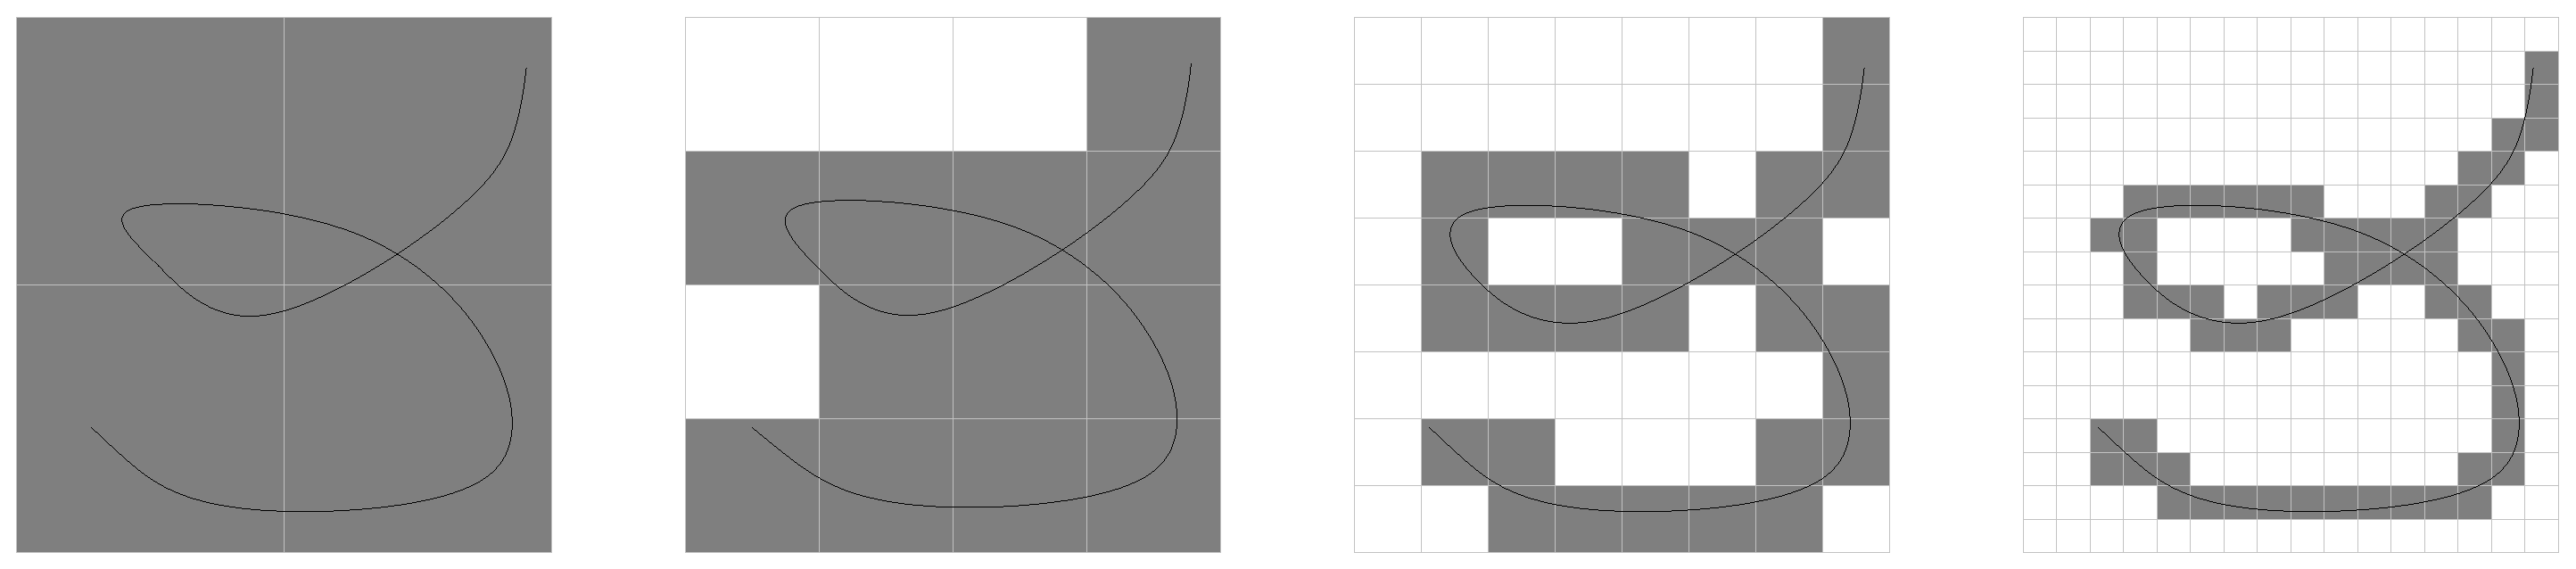
\includegraphics[width=12cm]{resolution}
\end{center}
\caption{R�le de  la r�solution pour une  coh�rence entre la topologie
  de   l'objet  continu  par rapport �     l'objet discret,  avec  une
  discr�tisation   en       supercouverture       (voir     paragraphe
  \ref{sec:discr-de-simpl}).\label{fig:resolution}}
\end{figure}




\subsection{Discr�tisations bas�es sur le maillage}
\label{sec:discr-class}

Consid�rons dans  un premier temps un  objet continu $F$ dont  le bord
poss�de  la  propri�t�   de \OldName{Jordan}   (c'est-�-dire  avec  un
int�rieur  et un ext�rieur).  Le   premier processus de discr�tisation
est d� �   \OldName{Gauss} pour  une    estimation d'aire de   l'objet
euclidien.  Le principe est le  suivant~: la discr�tisation de l'objet
correspond � l'ensemble des  points  de coordonn�es  enti�res contenus
dans $F$.   Ce  processus   est aussi  appel�    \emph{Object Boundary
  Quantization}      (OBQ).   


Dans  le cas d'une  discr�tisation de  courbe ne  disposant pas  de la
notion  d'int�rieur,   nous ne  pouvons �videmment pas  consid�rer  la
discr�tisation  de  \OldName{Gauss} ;   d'autres sch�mas existent pour
cela.   Nous   citons  ici   la  discr�tisation  \emph{Grid  Intersect
  Quantization}   (GIQ) qui approxime  la  courbe  par l'ensemble  des
pixels \emph{les plus  proches}  selon un certain  crit�re~: �  chaque
fois que  la  courbe croise une  ar�te  du maillage, deux pixels  sont
consid�r�s  et le  plus proche   de l'intersection  selon la  distance
euclidienne fait  partie  de la discr�tisation de  la  courbe (voir la
figure \ref{fig:disc_mail}).  Le cas  pathologique pour ce sch�ma  est
le cas  o� la courbe passe � �gale distance  des deux pixels.  Il faut
soit consid�rer  les deux points  (d'o�  l'apparition de \emph{bulles}
dans la   discr�tisation, voir  section  \ref{sec:discr-pavage}), soit
faire un choix syst�matique et arbitraire (par exemple \emph{ le pixel
  d'abscisse ou d'ordonn�e la   plus petite}).  Remarquons ici  que ce
choix rend  le   processus  de  discr�tisation non   invariant �   une
permutation des axes de la grille.


\begin{figure}[htbp]
\begin{center}
  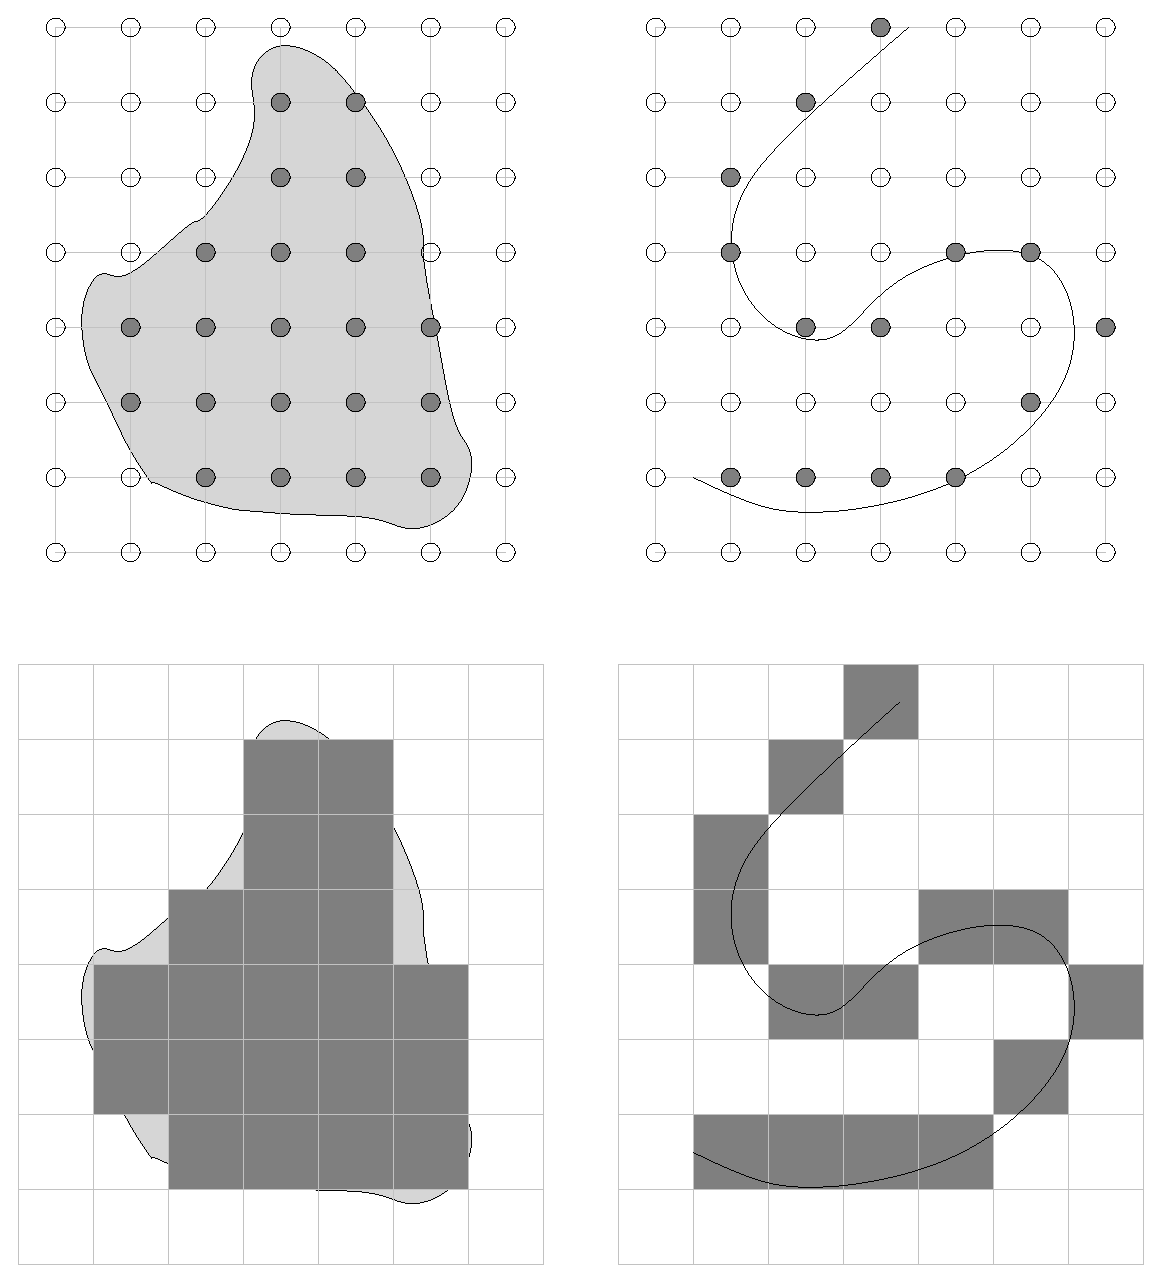
\includegraphics[width=7cm]{discretisations_maillage}
\end{center}
\caption{Processus  de  discr�tisation   classiques  sur  le  maillage
  (premi�re   ligne) ou  sur  le pavage  (seconde  ligne) : �  gauche,
  discr�tisation de \aut{Gauss} d'un objet  et � droite, discr�tisation GIQ d'une
  courbe.\label{fig:disc_mail}}
\end{figure}


Nous  pr�cisons  maintenant des  sch�mas   de discr�tisation sp�cifiques  aux
droites et plans discrets. Etant donn�e une droite $D$ dans le premier
octant (pente  positive inf�rieure � 1),  la discr�tisation GIQ de $D$
peut �tre vue comme un processus d'arrondi �  l'entier le plus proche.
En   effet, pour  $D:$  $y=\alpha   x+\beta$ par exemple,  les  points
de la discr�tisation sont donn�s par\footnote{$[x]$ d�signe
  l'arrondi  de $x$ � l'entier le  plus proche $x$.  De plus, $\lfloor
  x\rfloor$ (respectivement   $\lceil x\rceil$) correspond � l'entier inf�rieur
  (respectivement sup�rieur)  le  plus   proche  de   $x$.} :
\begin{displaymath}
\big   \{ (x_i,y_i)\;:\;  y_i=[\alpha x_i+\beta],\,x_i\in\Z \big \}\,,
\end{displaymath}

Par abus de langage, la discr�tisation :

\begin{displaymath}
\big   \{ (x_i,y_i)\;:\;  y_i=\lfloor \alpha x_i+\beta \rfloor,\,x_i\in\Z\big  \}
\end{displaymath}

est appel�e \emph{discr�tisation OBQ de $D$}. De m�me, la
discr�tisation :
\begin{displaymath}
\big   \{ (x_i,y_i)\;:\;  y_i=\lceil \alpha x_i+\beta \rceil,\,x_i\in\Z\big  \}
\end{displaymath}
est  appel�e\index{discr�tisation!Back@\emph{Background   Boundary  Quantization}}
\emph{discr�tisation BBQ  (Background Boundary Quantization)  de $D$}.
La figure \ref{fig:disc_droites} illustre ces diff�rents sch�mas.

\begin{figure}[ht]  
  \centering
  \includegraphics[width=12cm]{discretisations_droite}
  \caption{Diff�rents    sch�mas  de  discr�tisation  sp�cifiques  aux
    droites~: \emph{(de gauche � droite)} discr�tisations $GIQ$, $OBQ$
    et   $BBQ$.   Les    intervalles  repr�sentent    les   op�rations
    d'arrondi.\label{fig:disc_droites}}
\end{figure}
\subsection{Discr�tisations bas�es sur le pavage}
\label{sec:discr-pavage}


Nous  pr�sentons  tout d'abord  un  sch�ma  de discr�tisation,  appel�
\emph{supercouverture}, utilisant  la  repr�sentation par pavage \cite{bb33412,montanvert,andres_hdr}~:  la
discr�tisation d'un  objet   euclidien $F$  en supercouverture,  not�e
$\mathbb{S}(F)$ consid�re tous   les pixels (ferm�s) intersect�s par  $F$ (voir
figure  \ref{fig:disc_pav}).  Ce  sch�ma,   tr�s  simple,  d�finit  un
processus  de  discr�tisation valide  quel  que soit le type d'�l�ment
(courbe,  objet, point,  etc.).   Il permet  de   plus de montrer  des
propri�t�s  fondamentales  utiles  en  mod�lisation, par  exemple pour
l'assemblage d'objets.  Voici  quelques-unes   des  propri�t�s de   la
discr�tisation en supercouverture ~:

\begin{align*}
  &\mathbb{S}(F\cup G)=  \mathbb{S}(F) \cup
  \mathbb{S}(G)\,,\\
  &\mathbb{S}(F)= \bigcup_{p\in F} \mathbb{S}(p)\,,\\
  &\mathbb{S}(F\cap G)\subseteq  \mathbb{S}(F) \cap \mathbb{S}(G)\,,\\
  &\text{si } F\subseteq G\text{ alors }  \mathbb{S}(F) \subseteq \mathbb{S}(G)\,.
\end{align*}


Ce  processus est g�n�ralisable en dimension  sup�rieure, il suffit de
consid�rer   les    intersections de  la forme   avec   les  voxels ou les
hypercubes.  Cependant, cette discr�tisation produit
des objets  parfois �pais.  En effet,  si l'objet continu passe par un
sommet   du pavage  (coordonn�e   demi-enti�re),  toutes les  cellules
adjacentes �     ce sommet font partie de la discr�tisation ; on parle  alors de
\emph{bulles}  (voir    figure \ref{fig:disc_pav}).     Ainsi,      la
discr�tisation d'une  droite ne sera pas  une $(1)-$courbe comme on aurait
pu le souhaiter mais un $(1)-$objet.  Encore une fois, avec des conventions
d'orientation   dans   le   cas  d'une discr�tisation    de structures
lin�aires, nous  pouvons supprimer ces bulles.  Le  mod�le issu de ces
choix est  appel� \emph{mod�le standard} \cite{Andres_standard}.  Dans
ce  sch�ma,  la  discr�tisation  d'une  droite  est  bien  une courbe
$(1)-$connexe.  Comme dans  le cas du  choix fait  pour GIQ, l'orientation
choisie dans ce mod�le rend le processus non invariant aux sym�tries
par     rapport       aux  axes   de      la     grille.
\index{discr�tisation!standard}

% \begin{figure}[htbp]
%   \centering
%   \includegraphics[width=10cm]{bulle}
%   \caption{Illustration d'une bulle en 2D et du mod�le standard.}
%   \label{fig:bulle}
% \end{figure}

\begin{figure}[htbp]
\begin{center}
  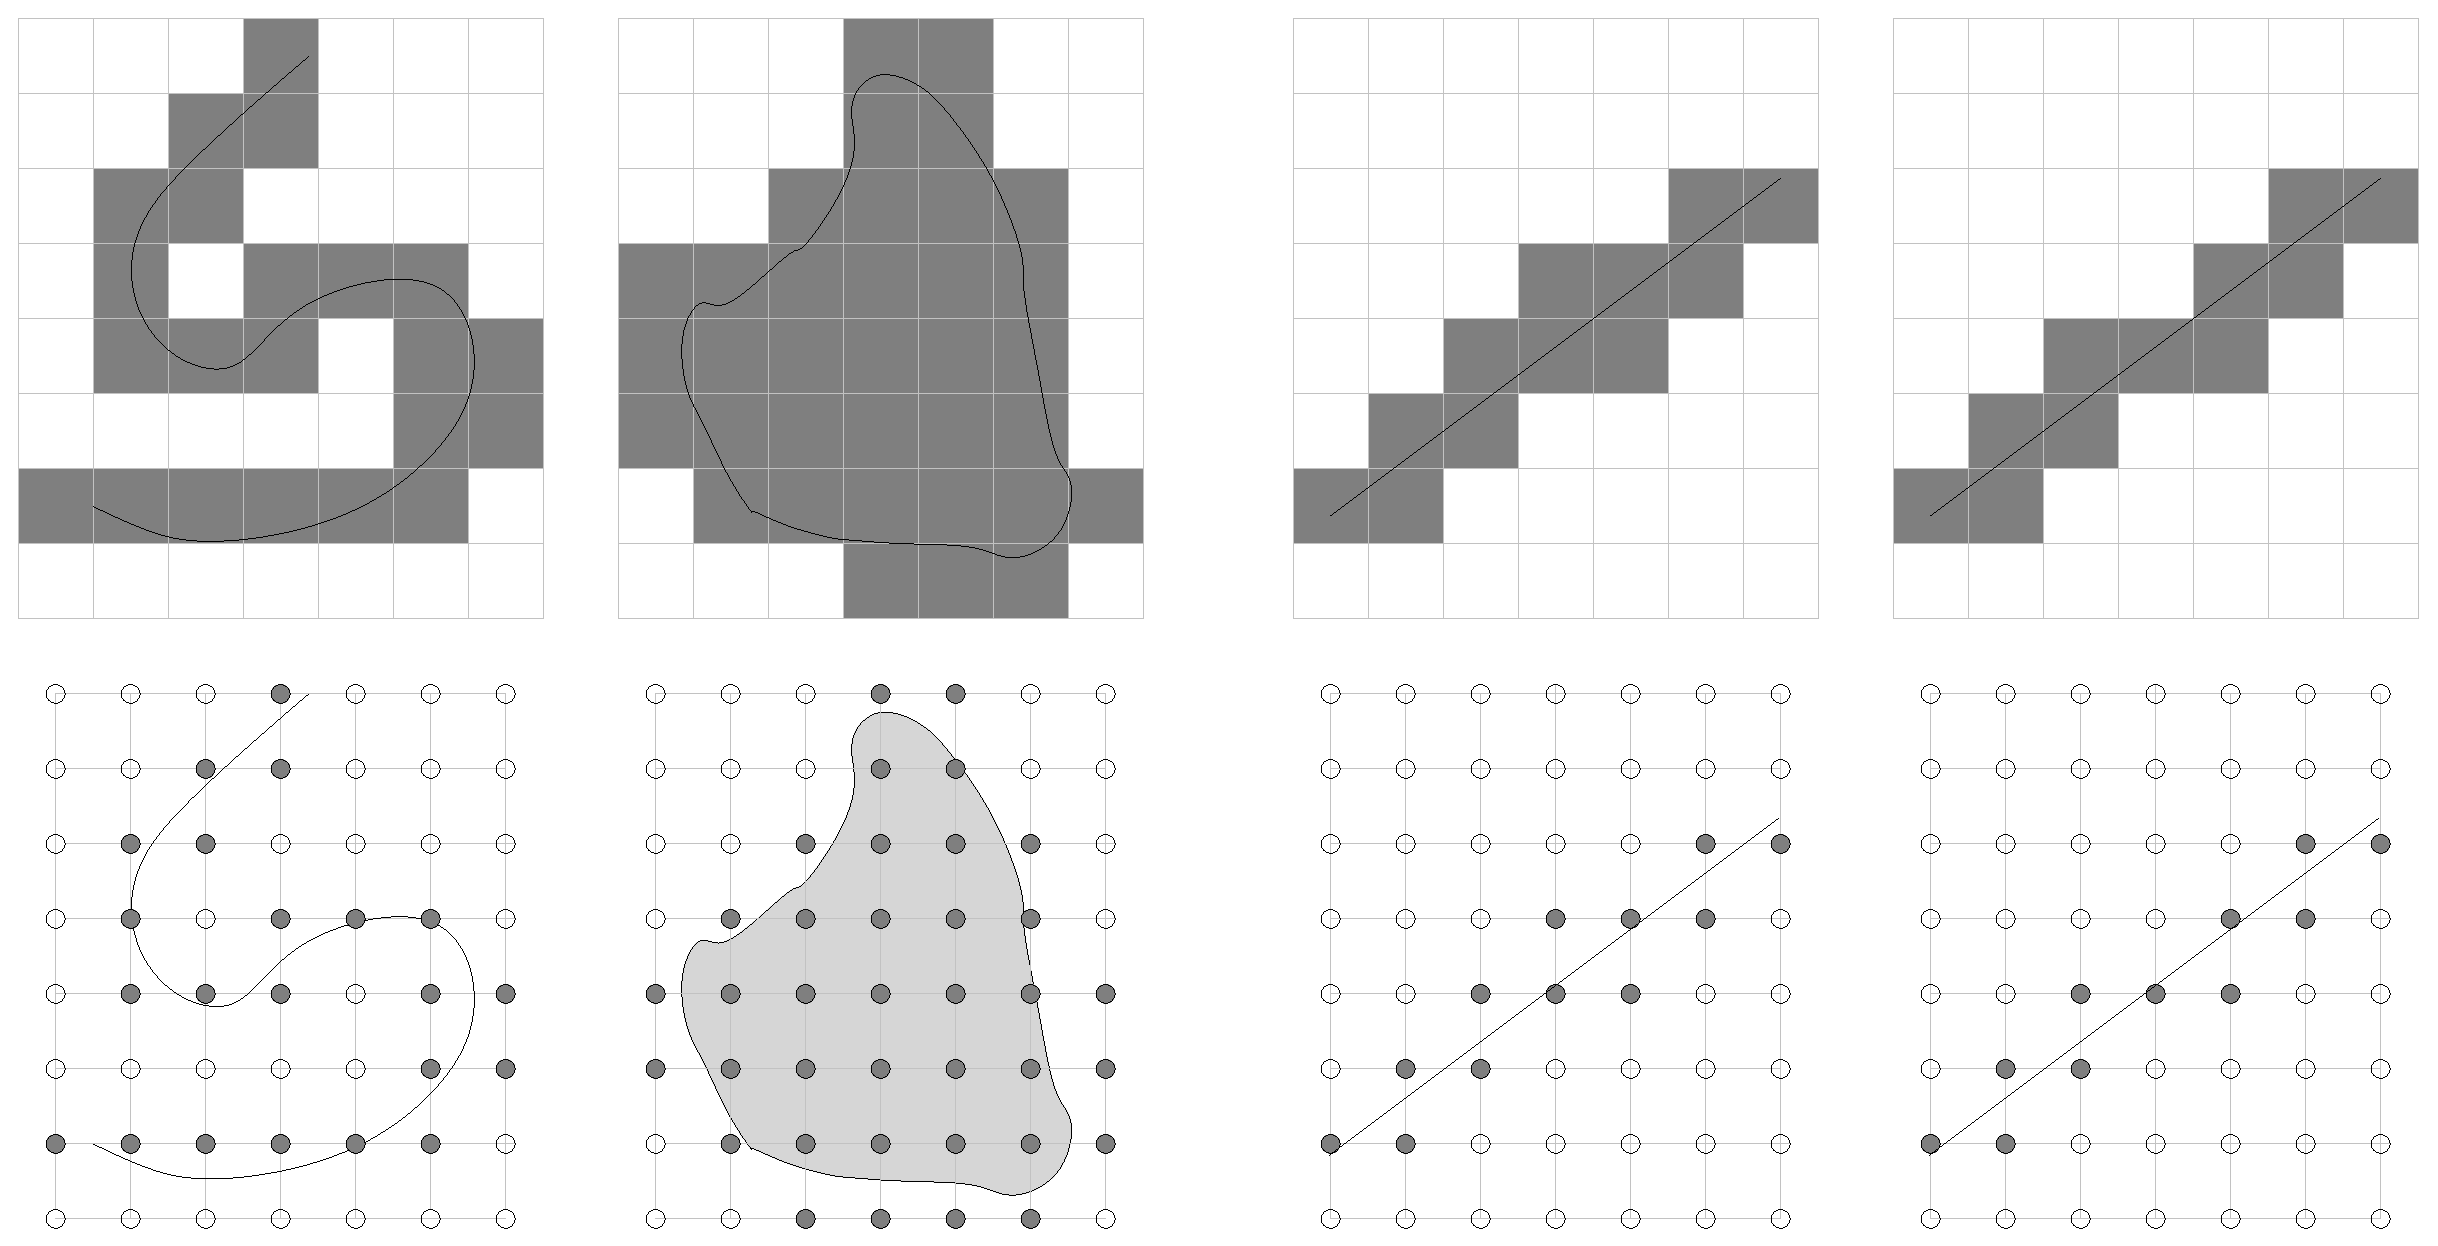
\includegraphics[width=12cm]{discretisations_pavage}
\end{center}
\caption{Processus de   discr�tisation   classiques  sur  le  pavage
    (premi�re  ligne) ou  sur le  maillage (seconde ligne)  : ({\it de
      gauche �    droite})   discr�tisation en  supercouverture  d'une
    courbe, discr�tisation  en supercouverture d'un   objet, illustration
    d'une bulle pour la discr�tisation   d'un  segment de droite,   et
    discr�tisation en mod�le standard.\label{fig:disc_pav}}
\end{figure}

\subsection{Mod�les analytiques discrets}
\label{sec:discr-de-simpl}
 

Dans la pr�sentation  pr�c�dente, nous pouvons g�n�raliser les sch�mas
de  discr�tisation en supercouverture   et   standard   en   d�finissant  un \emph{mod�le
  analytique discret}.  Pour cela, nous  n'allons plus nous int�resser
aux cellules du pavage qui sont  intersect�es par l'objet continu mais
� l'intersection entre l'objet et des r�gions convexes incluses dans
les pixels (voir figure \ref{fig:modeles}).
\index{discr�tisation!mod�le analytique}

Si la r�gion convexe est le pixel lui-m�me, nous retrouvons le mod�le de
supercouverture.   Si la r�gion   est un losange  centr�,  on parle de
\emph{mod�le  na�f ferm�}.   Enfin  si la r�gion  est un  disque, nous
d�finissons le \emph{mod�le pythagoricien} \cite{andres_hdr}.
\index{discr�tisation!na�f ferm�}
\index{discr�tisation!pythagoricien}

\begin{figure}[ht]
  \centering
  \includegraphics[width=12cm]{modele_analytique}
\caption{Quelques exemples de mod�les analytiques~: supercouverture,
  na�f ferm�, pythagoricien et engendr� par un pentagone.\label{fig:modeles}}
\end{figure}

% L'int�r�t de construire  un mod�le g�n�rique est  que l'on va  pouvoir
% prouver  des   propri�t�s g�om�triques  et topologiques (s�parabilit�,
% distributivit�  par rapport � l'union,  etc.)   pour tous les mod�les
% analytiques pour peu  que  la \emph{r�gion de base}  v�rifie certaines
% hypoth�ses   (convexit�,   connexit�   sur  $\mathbb{Z}^2$,     etc.)
% \cite{andres_hdr}.

Formalisons ces  mod�les~: nous consid�rons  une r�gion de base $C$ et
nous supposons  que cette r�gion correspond �  une boule de rayon
$\frac{1}{2}$ pour une certaine  distance $d$.  Par exemple, le  carr�
correspond �  la    boule  de rayon $\frac{1}{2}$   pour   la distance
$d_\infty(A,B)=\max\{|x_A-x_B|,|y_A-y_B|\}$,   le losange correspond �
la    boule    de   rayon    $\frac{1}{2}$     pour    la     distance
$d_1(A,B)=|x_A-x_B|+|y_A-y_B|$.  Nous notons $M$ l'�l�ment structurant
engendr� par la \emph{r�flexion} de $C$ par rapport � son centre.  Ces
notions d'�l�ment structurant  et de r�flexion viennent directement de
la morphologie math�matique \cite{serra}.  Le mod�le de discr�tisation
analytique $\mathbb{A}_C$ d'un objet euclidien $F$ est donn� par trois
d�finitions �quivalentes~:
\begin{align*}
  \mathbb{A}_C(F)&=\{A\in\Z^d~|~ C(A)\cap F \neq \emptyset\}\\
&=\{A\in\Z^d~|~ d(A,F)\leq \frac{1}{2}\}\\
&=(F\oplus M)\cap\Z^d
\end{align*}

La premi�re rejoint la d�finition que  nous avons donn�e pr�c�demment,
la seconde consid�re les points discrets � une certaine distance de la
forme  et  la derni�re  nous      donne une �criture relevant de  la  morphologie
math�matique o�  $\oplus$  correspond � la  somme  de \OldName{Minkowski}
\cite{serra,soillebook} de l'�l�ment  structurant $M$  et  de la forme  $F$.
Pour cette derni�re  d�finition, nous consid�rons les poins discrets
contenus  dans  la   forme   continue    $F\oplus M$    (voir   figure
\ref{fig:anal_generique}).

\begin{figure}[ht]
  \centering
  \includegraphics[width=12cm]{modele_analytique_generique}
  \caption{Illustration  des d�finitions  d'un mod�le analytique d'une
    forme quelconque: d�finitions par intersection avec les r�gions et
    par  morphologie  math�matique  ($C$  est  la  r�gion  et $M$   sa
    r�flexion       par      rapport            au    centre        de
    $C$).\label{fig:anal_generique}}
\end{figure}

Sur ce mod�le g�n�rique, nous retrouvons les propri�t�s~: 
\begin{align}
  &\label{eq:union}\mathbb{A}_C(F\cup G)=  \mathbb{A}_C(F) \cup
  \mathbb{A}_C(G)\,,\\
  &\label{eq:composition}\mathbb{A}_C(F)= \bigcup_{P\in F} \mathbb{A}_C(P)\,,\\
  &\label{eq:inter}\mathbb{A}_C(F\cap G)\subseteq  \mathbb{A}_C(F) \cap \mathbb{A}_C(G)\,,\\
  &\label{eq:inclusion}\text{si } F\subseteq G\text{ alors }  \mathbb{A}_C(F) \subseteq \mathbb{A}_C(G)\,.
\end{align}

Enfin, �tant donn�e  la  topologie  de l'objet   $F$,  des r�sultats
peuvent �tre  d�montr�s sur   la    topologie  de sa    discr�tisation
$\mathbb{A}_C(F)$  en consid�rant  des  propri�t�s  v�rifi�es par  la
r�gion $C$ \cite{andres_hdr,LinckeW03}.


\section{Arithm�tique d'intervalles et  supercouverture}

D�s les  premiers      pas de  l'informatique th�orique   (voire    des
math�matiques   discr�tes)   et  m�me    bien   avant la   r�alisation
\emph{physique} des ordinateurs,     s'est pos�  le   probl�me de   la
repr�sentation et de la manipulation de quantit�s r�elles. 

G�n�ralement, plusieurs sous-probl�mes peuvent �tre �nonc�s~:
\begin{itemize}
\item Comment repr�senter toutes les quantit�s r�elles ?
\item Comment faire des calculs num�riques sur ces repr�sentations ?
\item Quels contr�les peut-on mettre en place pour �valuer les
  approximations, s'il y a lieu, de ces calculs 
  approch�s  par rapport aux r�sultats \emph{exacts} ?
\item Comment  prendre une d�cision ou  tester la \emph{v�racit�} d'un
  pr�dicat bas� sur le r�sultat d'un calcul ?
\end{itemize}

Plus simplement, les deux premiers points reposent sur la constitution
d'une   arithm�tique.   Le troisi�me  point  fait   le lien entre  les
r�sultats approch�s par l'arithm�tique choisie et les r�sultats donn�s
par un mod�le de calcul exact.  Le dernier point est sans doute un cas
particulier   du pr�c�dent~:  une pr�dicat   simple  est une  fonction
prenant en  entr�e des nombres de   notre arithm�tique et  retournant un
bool�en.

En g�om�trie algorithmique, la notion  de pr�dicat est tr�s importante
et  la robustesse   de   l'�valuation de  ces    derniers  permet  des
impl�mentations  robustes d'algorithmes g�om�triques (la litt�rature est
tr�s dense sur  le sujet, voir  par exemple \cite{pion}).  Un pr�dicat
tr�s simple  et �  la base de beaucoup   d'algorithmes est le  pr�dicat
d'orientation de trois points dans le plan.


L'objet ici  n'est pas de pr�senter de  mani�re exhaustive  toutes les
solutions � ce  probl�me de repr�sentation.  Nous nous int�resserons �
des calculs et  pr�dicats certifi�s, dans le  sens  o� nous gardons  et
propageons les incertitudes tout  au long des  calculs par  l'usage de
l'arithm�tique d'intervalles  dont nous donnons  une interpr�tation en
g�om�trie discr�te.


\subsection{�l�ments de base}

Supposons le  codage des  nombres  en double  pr�cision d�fini dans la
norme  \textsc{IEEE 754}, tr�s utilis�e  dans les calculs num�riques~:
sur 64 bits codant un \emph{double}, nous  avons 1 bit de signe ($s$),
11 bits d'exposant  ($e$) et 52  bits de mantisse  ($m$).  Le nombre a
pour valeur $s\cdot  m\cdot  2^e$.  Bien �videmment,  tous les   nombres
r�els ne  peuvent �tre  repr�sent�s, on   note  donc $\mathbb{F}$  les
nombres repr�sentables  (auxquels   nous pouvons   ajouter $\{+\infty,
-\infty, NaN\}$).  Par cons�quence  de  la construction  des  doubles,
$\mathbb{F}$  n'est pas uniforme sur  $\mathbb{R}$ (les petits nombres
sont plus finement repr�sent�s que les grands).

Si nous consid�rons   un nombre r�el   $x$, si  $x$ est  repr�sentable
(\emph{i.e.} $x\in\mathbb{F}$), le double   associ� est  {\tt  x}$=x$.
Sinon, $x$  est entre  deux  nombres repr�sentables  successifs  not�s
$\overline{\tt   x}$ et $\underline{\tt  x}$.     Par la suite,  nous
noterons   $\sI{x}=  \ffup{x}$  et  $\iI{x}=\fdown{x}$  les  op�rateurs
permettant d'atteindre les   plus proches flottants  repr�sentables  de
$x$.  Pour terminer   avec la norme \textsc{IEEE  754},  l'utilisateur
choisit un  \emph{mode  d'arrondi} selon l'op�rateur $\ffup{\cdot}$  ou
$\fdown{\cdot}$ privil�gi�   dans  la   red�finition   des  op�rateurs
arithm�tiques  classiques.  Ainsi, le r�sultat    d'un calcul sur  les
nombres repr�sentables est un nombre repr�sentable.

En     arithm�tique   d'intervalles,  l'objectif    est   de  propager
l'incertitude que l'on a sur la repr�sentation d'un  r�el tout au long
du calcul \cite{Moor66a,Moore79a}.  Tout  r�el $x$ est repr�sent�  par
un intervalle $X$~:
\begin{displaymath}
  X= [\sI{x},\iI{x}]
\end{displaymath}

Nous  noterons   $\mathbb{I}_\mathbb{F}$ l'espace  engendr�    par les
intervalles  sur   les  nombres   repr�sentables  $\mathbb{F}$.   Pour
simplifier l'�criture,   nous  notons simplement $\mathbb{I}$  lorsque
l'espace \emph{support} des  intervalles  est, soit implicite   par le
contexte, soit que la validit� de  l'�nonc� ne d�pend pas de celui-ci.
En  dimension sup�rieure,   $\mathbb{I}^n$ est  le  produit  cart�sien
$\I\times\ldots\times\I$ de $n$ espaces.

Nous pouvons  d�river des  op�rateurs  tout  en assurant la  propri�t�
d'inclusion d'un op�rateur sur les intervalles~:

\begin{propriete}[Inclusion]
 Soit $f:\mathbb{R}\rightarrow\mathbb{R}$, notons $\Box f:
 \mathbb{I}\rightarrow \mathbb{I}$ la fonction associ�e � $f$ pour
 les intervalles. Pour tout $x\in X$, $\Box f$ v�rifiera la propri�t�~:
 \begin{displaymath}
   f(x)=y\quad \Rightarrow \quad y \in \Box f(X)
 \end{displaymath}
\end{propriete}

Ainsi, nous pouvons d�finir~:
\begin{align*}
  X\oplus Y &= [\fdown{\iI{x}+\iI{y}}, \ffup{\sI{x}+\sI{y}}]\\
  X \ominus Y &= [\fdown{\iI{x}-\sI{y}}, \ffup{\sI{x}-\iI{y}}]\\
  X\odot Y &=  [\min{(\fdown{\iI{x}\cdot\iI{y}},\fdown{\iI{x}\cdot\sI{y}},
    \fdown{\sI{x}\cdot\iI{y}},\fdown{\sI{x}\cdot\sI{y}})},\\&\max{(\ffup{\iI{x}\cdot\iI{y}},\ffup{\iI{x}\cdot\sI{y}},\ffup{\sI{x}\cdot\iI{y}}, \ffup{\sI{x}\cdot\sI{y}})}]
\end{align*}

Remarquons  l'usage des op�rateurs  $\ffup{\cdot}$  et  $\fdown{\cdot}$
permettant de construire  $\mathbb{I}$ sur $\mathbb{F}$, et  qu'ainsi,
les  op�rations $\min$ et  $\max$ se font  de mani�re exacte sur $\F$.
Notons aussi que, dans  le cas de la  multiplication, l'impl�mentation
directe  serait inefficace  (8   multiplications), en consid�rant  les
signes   des bornes,  nous   pouvons obtenir   une impl�mentation plus
efficace \cite{Moore79a}.  Selon  ces  d�finitions, l'addition  et  la
multiplication sont associatives et commutatives mais nous n'avons pas
la distributivit�, en effet~:
\begin{displaymath}
  X\odot (Y \oplus Z) \subset  (X\odot Y)\oplus (X\odot Z)\,.
\end{displaymath}

A partir  de ces op�rateurs  (que   nous pouvons compl�ter),  diverses
\emph{extensions}   sont possibles  tout  en  maintenant  la propri�t�
d'inclusion.  La plus simple  est l'extension naturelle~: si $f=g\circ
h$ alors $\Box f = \Box g \circ \Box h$. Il est clair qu'il existe une
infinit� d'extensions possibles   de fonctions r�elles.   Une  propri�t�
essentielle, en plus de la  propri�t� d'inclusion, est la propri�t� de
monotonicit� pour l'inclusion  d'intervalles~: si $X\subset  Y$, alors
nous devons avoir $\Box f(X) \subset \Box  f(Y)$.  De cette propri�t�,
nous pouvons d�river une notion de convergence tr�s utile lorsque nous
construisons  un solveur en   arithm�tique d'intervalles (voir section
\ref{sec:solv-en-arithm}).

Une autre propri�t� de l'extension souhaitable mais plut�t difficile �
atteindre est l'optimalit� (ou    minimalit�). Si cette derni�re   est
valide,   alors, pour tout intervalle $X$, il n'existe pas
d'intervalle $Y\subset \Box f(X)$ pour lequel la propri�t� d'inclusion
reste valide ($\forall x\in X, f(x)\in Y$).



Les  op�rateurs  $\oplus$, $\ominus$ et    $\odot$ sont monotones  par
inclusion et optimaux.  L'extension  naturelle est aussi monotone mais
non  optimale \cite{Moor66a,Moore79a}.  En effet, soit $f(x,y)=x*y-x$,
son extension naturelle est $\Box  f(X,Y)=X\odot Y \ominus X$, or pour
$X=[-2,2]$ et    $Y=[-1,5]$, $F(X,Y)=[-12,12]$.   Cependant   $[-8,8]$
v�rifie quand m�me la propri�t�  d'inclusion.  $\Box f$ n'est donc pas
optimale.  Cet exemple  nous permet aussi d'illustrer la probl�matique
de r��criture syntaxique et  symbolique des expressions pour optimiser
et contr�ler  la propagation des  erreurs  dans les calculs~: si  nous
notons    $f(x,y)=x*(y+1)$,     son    extension   naturelle     $\Box
f(X,Y)=X\odot(Y\oplus  [1,1])$   est   elle  optimale.    Nous pouvons
formaliser un   peu   plus ce fait  en   reformulant  le  th�or�me  de
\aut{Moore} \cite{Moor66a} (sous l'hypoth�se que les op�rateurs de
base soient optimaux)~:
\begin{propriete}[\cite{Moor66a}]
  Soit $f:\R^n\rightarrow  \R$  et $\Box  f: \I^n\rightarrow  \I$  son
  extension naturelle. Si toutes les variables n'apparaissent qu'une
  seule fois dans l'expression arithm�tique de $f$, alors $\Box f$ est
  optimale.
\end{propriete}


D'autres extensions existent, par exemple, si nous cherchons �
calculer l'extension de $f$ sachant $g=\nabla f$, nous pouvons utiliser
une version sur intervalle du th�or�me de la valeur moyenne~:
\begin{displaymath}
  \Box f(X) = f(Mid(X)) \oplus \Box g(X)\odot (X \ominus Mid(X))
\end{displaymath}
$Mid(X)$ �tant la valeur  milieu de l'intervalle  $X$.  On parle alors
\emph{d'extension centr�e} \cite{Moor66a,mo:RatschekRokne:84}. Cette extension  correspond
au d�veloppement de \aut{Taylor} d'ordre 1 et des g�n�ralisations aux
ordres sup�rieurs sont possibles. L'int�r�t de ces extensions est que
m�me si l'optimalit� ne peut �tre prouv�e, les intervalles sont
g�n�ralement plus pr�cis qu'avec une extension naturelle.


\begin{figure}[t]
  \centering
  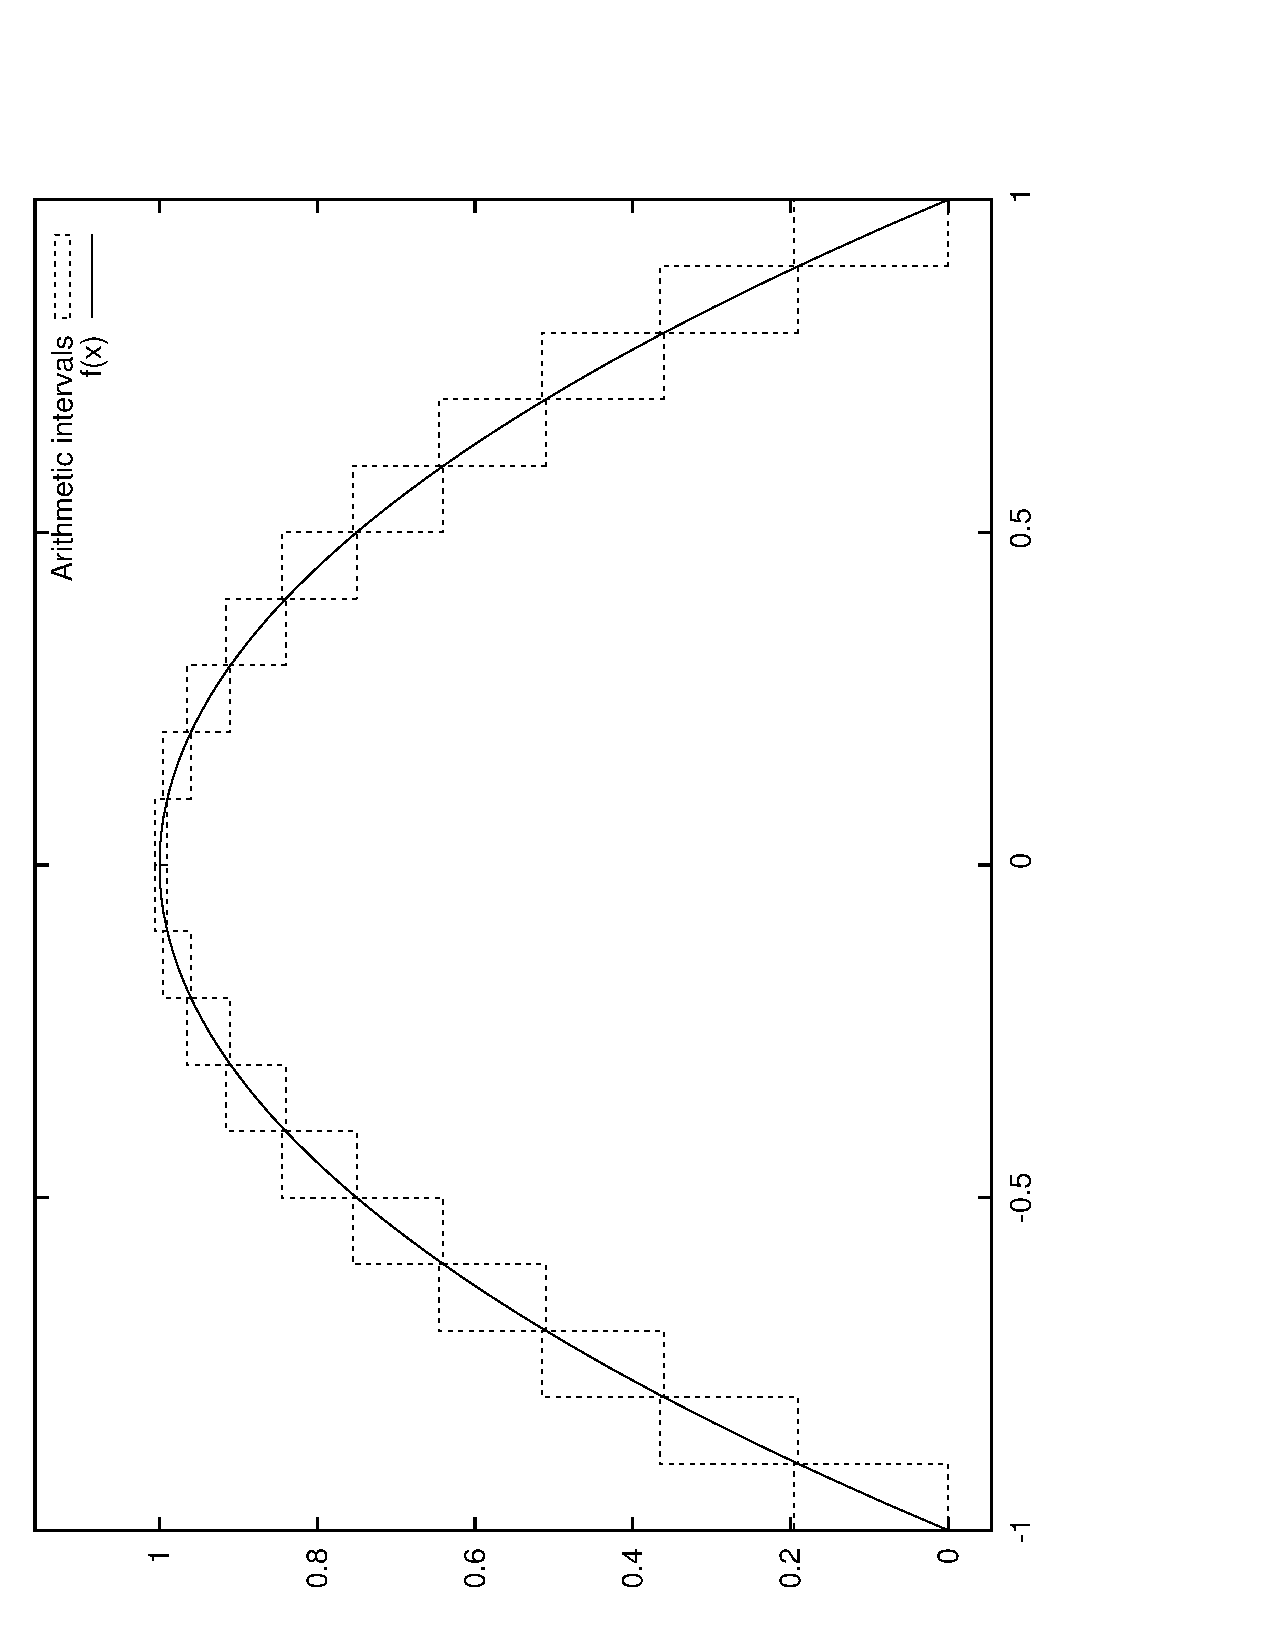
\includegraphics[angle=270,width=8cm]{IA_gnuplot}
  \caption{Analyse par arithm�tique d'intervalles $\I_\F$ de la fonction
    $f(x)=(x+1)(x-1)$ sur $[-1,1]$ par des intervalles
    $\{X_i\}_{i=1\ldots 20}$ de taille
    1/10.}
  \label{fig:IA}
\end{figure}

La figure \ref{fig:IA} pr�sente une analyse d'intervalles d'une courbe
simple.    Notons que si la  propri�t�  d'inclusion est toujours vraie
tout au long du calcul et qu'elle permet donc de prendre des d�cisions
ou de construire des pr�dicats exacts, la propagation des incertitudes
(c'est-�-dire   la    \emph{largeur}    des  intervalles)    peut �tre
probl�matique.  Pour   illustrer   cela, l'exemple classique   est  le
suivant  (exemple       de       \aut{Rump})~:     cherchons � �valuer
$f(x,y)=333.75y^6+x^2(11x^2y^2-y^6-121y^4-2)+5.5y^8+\frac{x}{2y}$,
pour $x=77617$ et $y=33096$,  sachant que le r�sultat \emph{exact} est
pour   les   premi�res d�cimales,   de   $-0.827396$.    Sur certaines
arithm�tiques   (ex.     OpenOffice Calc  ou   Excel),  nous  obtenons
$5.64\cdot  10^{40}$.  Avec une  arithm�tique  d'intervalles bas�e sur
les     doubles\footnote{\url{http://www.losderover.be/old/Easyval/}},
nous obtenons $[-5.90296\cdot  10^{21}, 4.72237\cdot 10^{21}]$.  donc,
bien que l'incertitude  de l'intervalle soit  tr�s grande, il n'en  est
pas moins vrai que ce dernier contient le r�sultat exact.




\subsection{Solveur en arithm�tique d'intervalles}
\label{sec:solv-en-arithm}

Un solveur en   arithm�tique   d'intervalles  consiste,  de    mani�re
g�n�rale, �    r�soudre     un     syst�me    $f$    sur  les    r�els
$\mathbb{R}^n\rightarrow\mathbb{R}$ sous forme implicite, c'est-�-dire
que nous cherchons  les  valeurs $\{(x_1,\ldots,x_n)\}$  pour lesquels
$f(x_1,\ldots,x_n)=0$.  Pour cela,  l'id�e  est d'utiliser l'extension
$\Box  f$, et de  rechercher les lieux   de  l'espace, c'est-�-dire les
hyper-intervalles   $\{X_i\}$ de dimension    $n$ tels que  $0\in \Box
f(X_i)$.

L'id�e est de proc�der par une recherche dichotomique (voir algorithme
\ref{solverIA})~:     en  partant     d'un  hyper-intervalle   initial
$X\in\mathbb{I}^n$, nous allons subdiviser r�cursivement ce domaine en
rejetant tous les sous-domaines  ne contenant pas la solution. L'arr�t
se fait par l'�valuation d'une fonction $\Box  A(X)$ qui, par exemple,
retourne    un intervalle contenant 1  tant   que l'intervalle $X$ est
d'�paisseur sup�rieure �  une  constante $\epsilon$  (l'�paisseur d'un
hyper-intervalle �tant la   plus grande  largeur  de ses   intervalles
mono-dimensionnels).  Ce param�tre r�gle  la finesse  de l'encadrement
des   solutions.  En contrepartie,  la r�currence est d'autant plus
longue que l'�paisseur souhait�e est petite.

Sur   ce sch�ma g�n�ral,   de   nombreux choix ou  optimisations  sont
possibles comme par exemple le choix entre une liste ou une file pour
$L$ (exploration en profondeur ou en largeur  d'abord), le choix de la
variable lors de la bissection,\ldots 

\begin{algorithm}[H]
  \Donnees{l'extension $\Box f$, un hyper-intervalle initial $X$ et
    une fonction d'arr�t $\Box A$}
  \Res{Une liste $S$ d'hyper-intervalles $\{X_i\}$ tels que $0\in \Box f(X_i)$}
  Placer $X$ dans une liste $L$\;
  \Tq{$L$ n'est pas vide}{
    Extraire un hyper-intervalle $X'$ de $L$\;
    Evaluation de $\Box f(X')$
    
    \Si{$0\in\Box f(X')$} {
      \eSi{$1 \in \Box A(X)$}{
        Bissection de l'hyper-intervalle $X$ selon une variable $x_k$
        en deux sous-hyper-intervalles $X'$ et $X''$\;
        Ajout de  $X'$ � $L$\;
        Ajout de  $X''$ � $L$
      }{Ajout de $X$ � $S$}
    }
  }
  
  \caption{\label{solverIA}Solveur na�f en arithm�tique
    d'intervalles  \cite{snyder-92}}
\end{algorithm}

En informatique graphique, ce  solveur peut-�tre utilis� pour le trac�
de courbes et de  surfaces   implicites \cite{snyder-92}.  N�anmoins,  des
solveurs   plus �labor�s  sont �tudi�s   dans   la   communaut�     de
programmation par     contraintes dans le cas   de   la  r�solution de
contraintes  non-lin�aires   sur  les  r�els    (voir par    exemple
\cite{bruynooghe1994cir,journals/rc/RueherS97}).

Etant donn�  que nous  pouvons  d�finir, pour  cette arithm�tique, des
op�rateurs   ensemblistes   (intersection,  union,\ldots)   ou  encore
bool�ens, l'extension $\Box  f$ peut �tre  complexe.  Par  exemple,
nous  pouvons ainsi  mod�liser   l'union ou  encore l'intersection  de
formes implicites  et utiliser le  solveur pr�c�dent  pour avoir
une approximation de la solution.

\subsection{Lien avec un mod�le analytique discret de supercouverture}

D'un  point  de vue   conceptuel,  la  propri�t� d'inclusion  dans les
mod�les    analytiques  discrets  (�quation \ref{eq:inclusion})  est �
mettre  en relation   avec la   propri�t�  d'inclusion, fondement   de
l'arithm�tique d'intervalles~:  dans  les  deux   mod�les, nous  avons
toujours une  inclusion  de l'objet continu   sous-jacent.   L� o�  le
mod�le analytique   discret propose une  construction  g�om�trique des
objets    (intersection    avec   un �l�ment  structurant,  distance �
l'objet,\ldots), les intervalles  proposent  une analyse arithm�tique,
voire alg�brique.

Pour  avancer un  peu sur les  liens entre   ces mod�les,  nous allons
consid�rer      l'arithm�tique  $\I_{\Z+\frac{1}{2}}$ d�finissant  les
intervalles sur les   demi-entiers  (nombres $k  + \frac{1}{2}$,  pour
$k\in\Z$). Ce d�calage  de $\frac{1}{2}$  nous  permet de  centrer les
intervalles sur les points discrets.  Les intervalles se construisent
de la mani�re suivante~:

\begin{align*}
\text{si }  &k \in \Z \,,\quad K= \left[ k-\frac{1}{2},k+\frac{1}{2}\right]\,.
\end{align*}

Lorsqu'un nombre est donn� sur les r�els ou lors de la d�finition d'un
op�rateur arithm�tique, nous d�finissons les op�rateurs~:
\begin{align*}
  \ffup{x} &= \left \lceil x+\frac{1}{2} \right \rceil -\frac{1}{2}\,, \\
  \fdown{x}&=\left \lfloor x+\frac{1}{2} \right \rfloor -\frac{1}{2}\,. \\
\end{align*}

De mani�re simple, nous  pouvons d�river les op�rateurs  arithm�tiques
sur cet espace $\I_{\Z+\frac{1}{2}}$.  Prenons  l'exemple trac� sur la
figure~\ref{fig:iia}-(a)  de  la     fonction   $f(x)=\frac{1}{2}x+1$,
l'analyse de $\Box f$ pour les intervalles de taille 1 centr�s sur les
points discrets  nous donne exactement le m�me  r�sultat que  le trac�
$\S(f)$,  modulo  le fait que deux   pixels align�s verticalement dans
$\S(f)$ nous donnent pour $\Box f$ un simple intervalle de hauteur 2.


Avant   de formaliser  les  interactions entre   ces mod�les,  il faut
cependant   r�gler   le  probl�me  des   \emph{bulles} (voir   section
\ref{sec:discr-pavage}).    En effet, dans   notre espace  support des
bornes des  intervalles, $\Z+\frac{1}{2}$,  si  $x$ est  repr�sentable
(c'est-�-dire  sous  la forme $k+\frac{1}{2}$  pour  $k\in\Z$), il est
d'usage  dans   les  biblioth�ques  impl�mentant    les  arithm�tiques
d'intervalles  de consid�rer l'intervalle   de largeur  nulle  $[x,x]$
(afin de supprimer une incertitude qui se propagerait inutilement dans
les  calculs).  L'inconv�nient dans  notre  mise en  relation avec  le
mod�le   supercouverture  est que    lors  du   trac�  sur  la  figure
\ref{fig:iia}-(b)  avec la fonction, $f(x)=\frac{1}{3}x$ supprimera de
mani�re intrins�que toutes les bulles, en violation avec les principes
de    construction,  notamment  morphologiques,   de   $\S(f)$.   Nous
choisissons  donc   de contraindre notre  arithm�tique  pour retourner
l'intervalle $[x-1,x+1]$ si $x\in\{\Z+\frac{1}{2}\}$.

\begin{figure}[ht]
  \centering
\subfigure[]{\includegraphics[angle=270,width=6.5cm]{trace_iia_classique}}
\subfigure[]{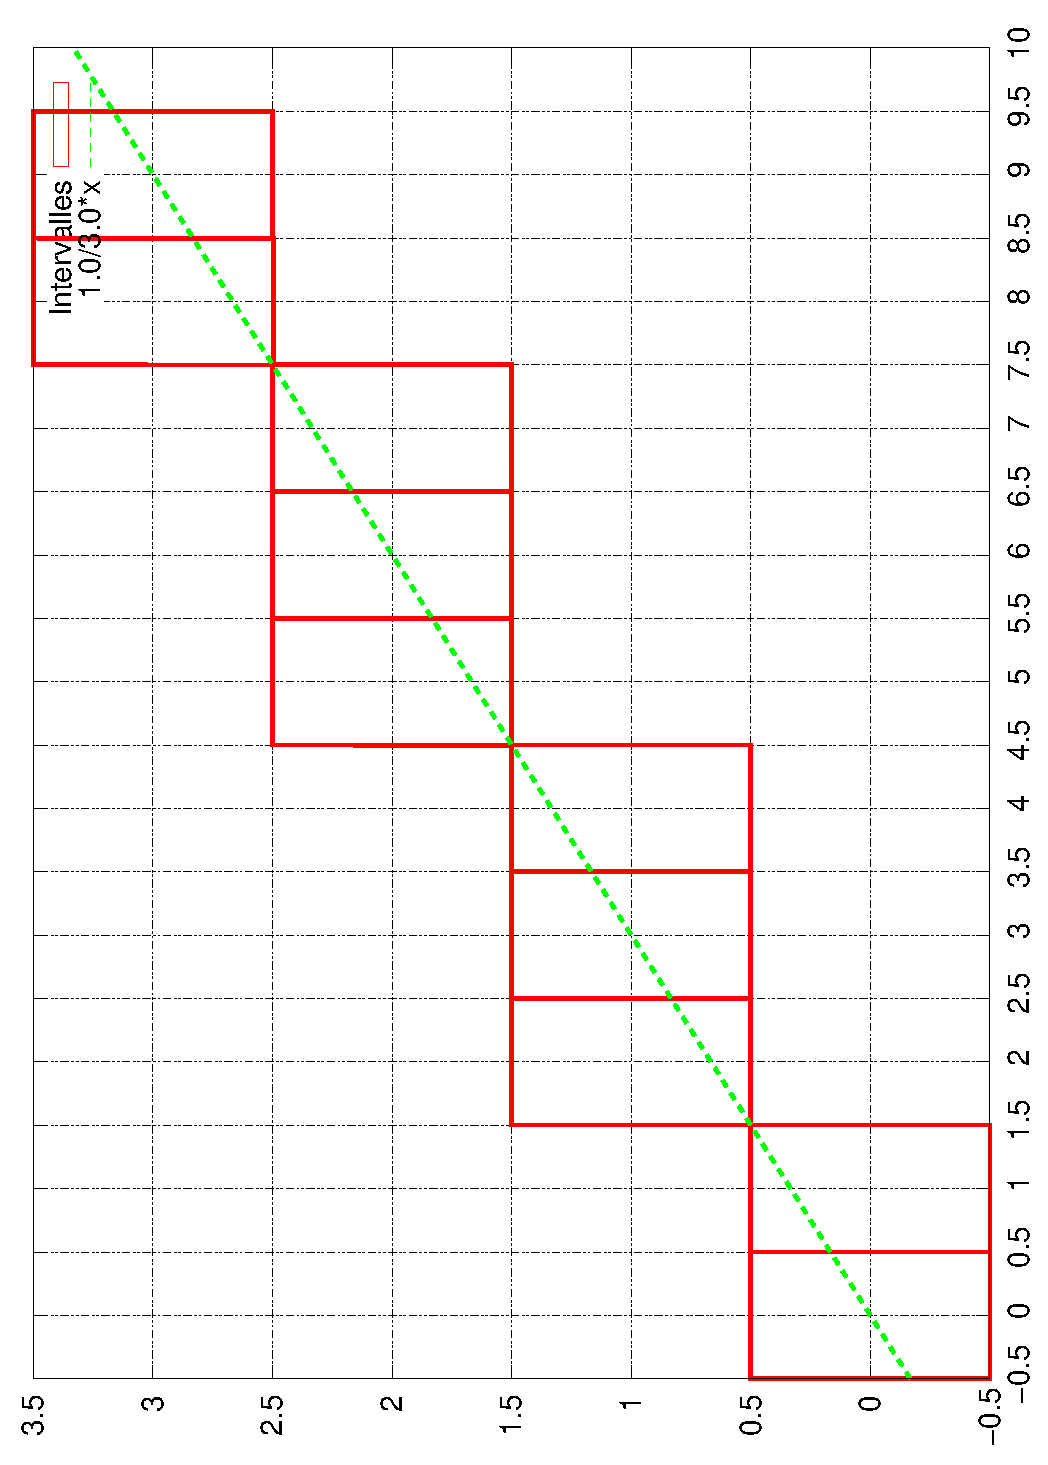
\includegraphics[angle=270,width=6.5cm]{trace_iia_classique_sansbulle}}
\caption{Trac� en arithm�tique d'intervalles $\I_{\Z+\frac{1}{2}}$ des
  fonctions $f(x)=\frac{1}{2}x+1$ $(a)$ et $f(x)=\frac{1}{3}x$ $(b)$.}
  \label{fig:iia}
\end{figure}

Avec ce  choix sp�cifique, nous  obtenons des algorithmes de  trac� de
fonctions tr�s simples (voir figure \ref{fig:iia_autres}).  Remarquons
sur  la figure  \ref{fig:iia_autres}-(a)  la pr�sence  de bulles (m�me
fonction   que  pour    la   figure   \ref{fig:iia}-(b)).   La  figure
\ref{fig:iia_autres}-(b)  illustre l'utilisation  d'op�rateurs    plus
complexes.  La figure  \ref{fig:iia_nonopt} illustre diff�rents trac�s
pour lesquels l'arithm�tique d'intervalles n'est pas optimale.




\begin{figure}[ht]
  \centering
  \subfigure[]{\includegraphics[angle=270,width=6.5cm]{trace_iia_classique_avecbulle}}
  \subfigure[]{\includegraphics[angle=270,width=6.5cm]{trace_iia_exp}}
\caption{Trac�  en arithm�tique d'intervalles $\I_{\Z+\frac{1}{2}}$
  modifi�e, des fonctions  $f(x)=\frac{1}{3}x$ et $f(x)=10\sin(x)\exp^{-x^2/50}$.}
  \label{fig:iia_autres}
\end{figure}


\begin{figure}[ht]
  \centering
\subfigure[]{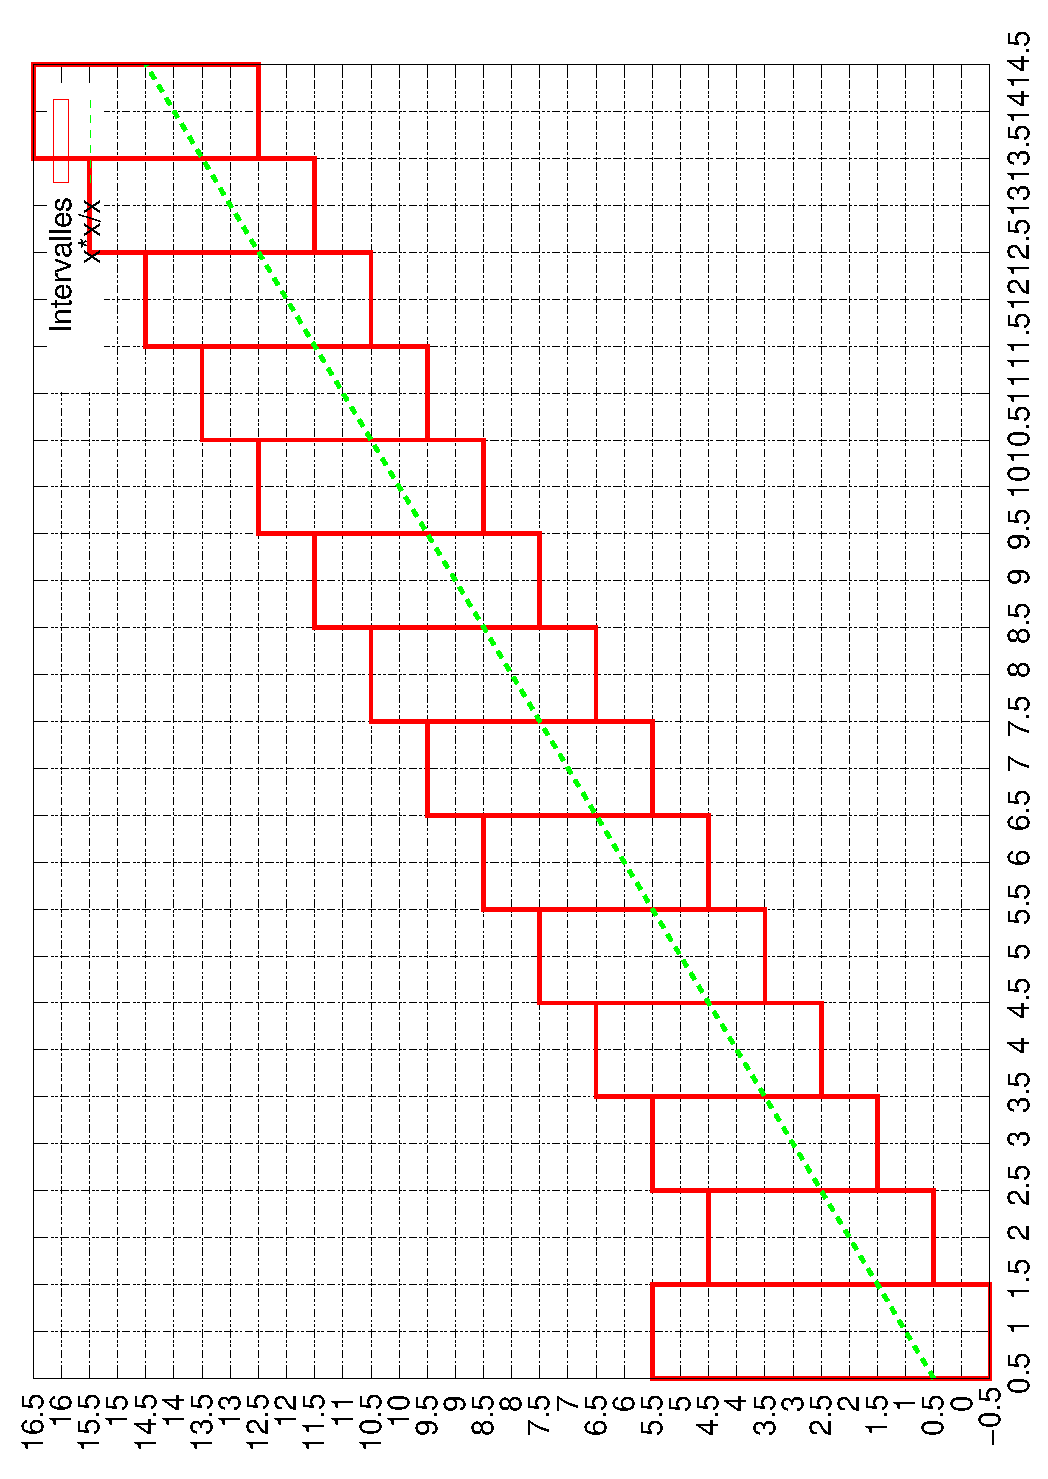
\includegraphics[angle=270,width=6.5cm]{trace_iia_nonoptim}}
\subfigure[]{\includegraphics[angle=270,width=6.5cm]{trace_iia_nonoptim2}}
  \caption{Exemple de trac� avec des extensions non optimales~:$(a)$
    $f(x)=\frac{x^2}{x}$ et $(b)$ $g(x)=h(h(x))$ avec $h(x)=\frac{\sqrt{x^2-x+1/2}}{\sqrt{x^2+1/2}}$.}
  \label{fig:iia_nonopt}
\end{figure}

Nous pouvons maintenant formaliser plus pr�cis�ment les liens entre la
supercouverture et l'analyse par  intervalles.  Dans le lemme suivant,
l'inclusion et    l'�galit�  sont �  prendre  au   sens  g�om�trique~:
inclusion ou �galit� des r�gions   du plan engendr�es par  l'union  de
cellules ferm�es de la grille pour la supercouverture, et l'union des
hyper-intervalles 2D pour l'arithm�tique d'intervalles.


\begin{lemme}
\label{lem:IA}
  Supposons  l'arithm�tique   sur  $\I_{\Z+\frac{1}{2}}$  et   $f:  \R
  \rightarrow \R$  une  application continue,  alors\footnote{$K$  est
    l'intervalle   $\left[    k-\frac{1}{2},k+\frac{1}{2}\right]$ pour
    $k\in\Z$.}~:
$$\S(f) \subseteq \bigcup_{k\in\Z} [K\times \Box f(K)]\,. $$
 

Si $\Box f$ est optimale sur $\I_{\Z+\frac{1}{2}}$, alors~:
$$ \S(f) =  \bigcup_{k\in\Z} [K\times \Box f(K)]\,.$$
\end{lemme}


\begin{mapreuve}
  Consid�rons    un    intervalle    centr�    sur  l'abscisse    $k$:
  $K=[k-\frac{1}{2},k+\frac{1}{2}]$.  Nous notons $Y=\Box f(K)$.  Soit
  $C$ une cellule de  $\S(f)$ centr�e sur l'abscisse $k$. �tant  donn�
  que  $\S(f)$  est   l'ensemble   des cellules  du   pavage  r�gulier
  intersectant  l'objet continu, il existe $x\in  K$ tel que $f(x)\cap
  C\neq\emptyset$.    Par     ailleurs et     par   d�finition      de
  $\I_{\Z+\frac{1}{2}}$,      $f(x)      \in    Y$     mais      aussi
  $[\fdown{f(x)},\ffup{f(x)}] \subseteq Y$.   Par d�finition du mod�le en
  supercouverture,         $C$ �tant             d�fini            par
  $[k-\frac{1}{2},k+\frac{1}{2}]\times[\fdown{f(x)},\ffup{f(x)}]$, nous
  concluons que $C\subseteq Y$ et donc $\S(f)\subseteq \Box f$.\\


  Pour montrer l'�galit�  si  $\Box  f$  est optimale,  supposons  une
  cellule                                                          $C:
  [k-\frac{1}{2},k+\frac{1}{2}]\times[l-\frac{1}{2},l+\frac{1}{2}]$
  telle que $C\subset Y$ et   telle que $l-\frac{1}{2}$ soit aussi  la
  borne   inf�rieure de  $Y$.   Nous montrons   que si $C\not\subseteq
  \S(f)$ alors $C\not\subseteq  \Box f(K)$.  Si $C\not\subseteq\S(f)$,
  alors pour tout $x\in K$, $f(x)\cap C=\emptyset$.  Donc il existe un
  intervalle $Y'=Y /C$ ($Y'$ est donc de la forme $[l+\frac{1}{2}, p]$
  avec $p\in\Z+\frac{1}{2}$) tel que pour tout  $x\in K$, $f(x)\in Y$,
  contredisant   le fait  que     $\Box f$   soit  optimale.    Ainsi,
  $C\not\subseteq  \Box  f(K)$.   Un  raisonnement similaire peut �tre
  donn� dans le cas  o� la  borne sup�rieure  de $C$ co�ncide  avec la
  borne  sup�rieure de $Y$.  Le dernier  cas � traiter est lorsque $C$
  n'est pas  une extr�mit� de $Y$.  Dans  ce cas  et par continuit� de
  $f$, il   n'existe pas de cellules  $C'$  au-dessus de $C$  et $C''$
  en-dessous   telles  que $C'$  et  $C''$   appartiennent tous deux �
  $\S(f)$  et   non   $C$.   Ainsi,  si   $C\not\subseteq\S(f)$  alors
  n�cessairement, ou bien   toutes les cellules  en-dessous de  $C$ ne
  sont  pas  dans $\S(f)$,  ou   alors c'est  le   cas pour  celles
  au-dessus de $C$.  Nous pouvons donc nous  ramener dans le cas de la
  preuve o�  nous  restreignons $Y$ par  une  de ces  extr�mit�s (voir
  figure \ref{fig:preuve}).
  \begin{figure}[h]
    \centering
    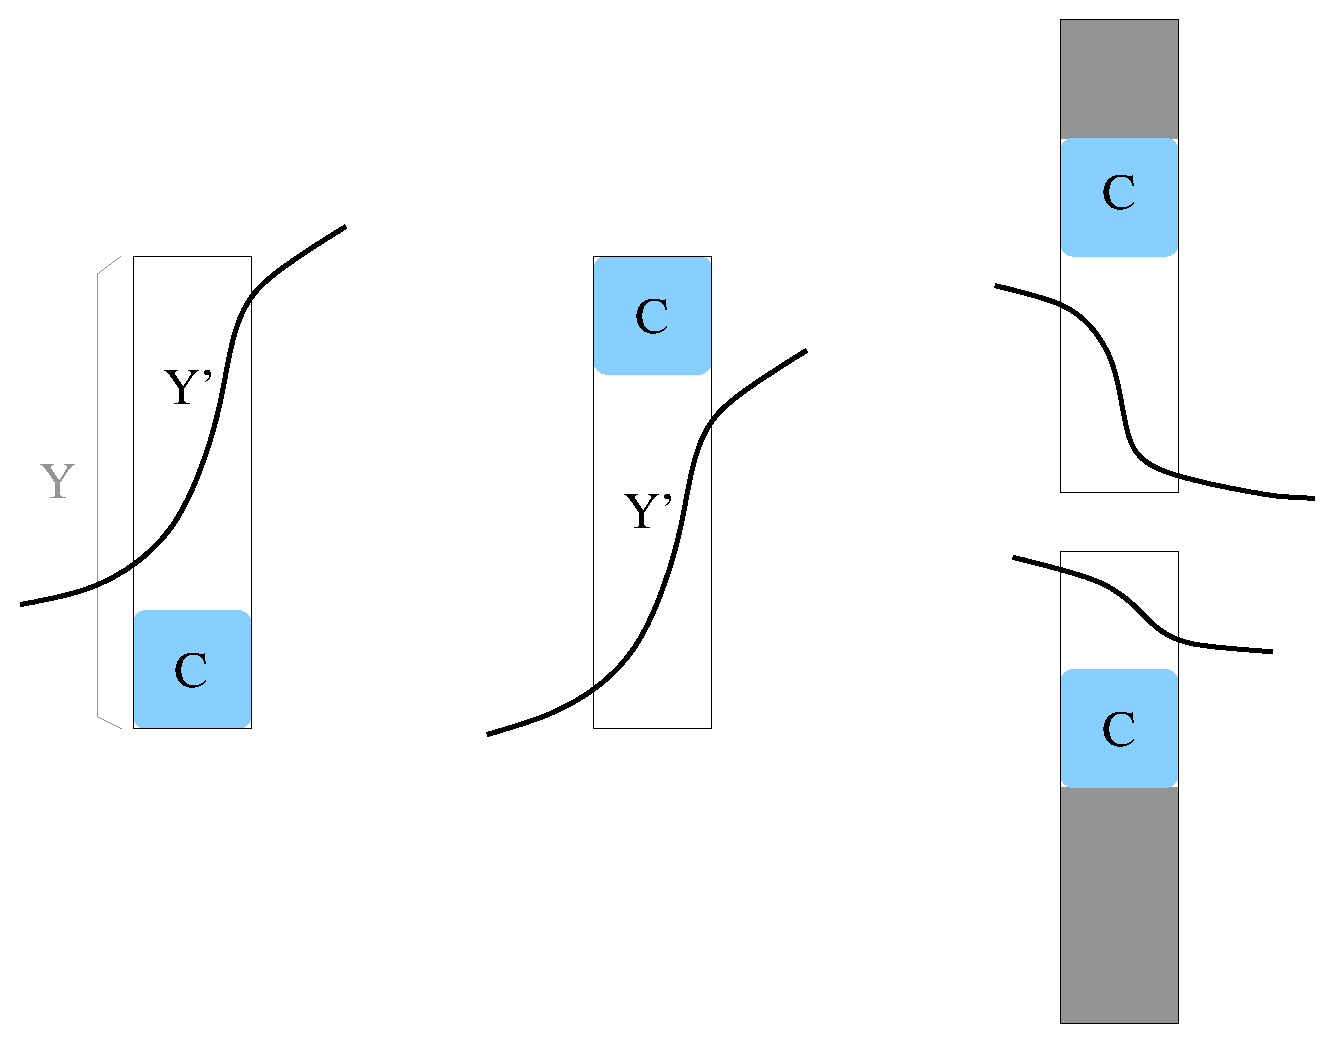
\includegraphics[width=8cm]{preuve_IA}
    \caption{Illustration de la preuve du lemme \ref{lem:IA}~: les
      diff�rents cas de  position de $C$ dans $Y$.}
    \label{fig:preuve}
  \end{figure}

\end{mapreuve}

Ce  lemme tr�s  simple      nous  permet  d'ajouter  au  mod�le     de
supercouverture, en    plus   des  caract�risations   g�om�triques,  de
morphologie   math�matique   ou    de distance, une    caract�risation
arithm�tique par l'usage d'op�rateurs sur  les intervalles. Notons que
nous  pouvons  tr�s  simplement   g�n�raliser ce  lemme   en dimension
sup�rieure.

La  figure  \ref{fig:iia_nonopt}  illustre  le  cas de trac�  avec des
extensions non-optimales.  Si l'inclusion $\S(f)\subseteq \Box  f$ est
bien �videmment  v�rifi�e,  les propagations d'erreurs peuvent produire
des encadrements tr�s grands de la solution. 



\section{Conclusion}

Dans ce  chapitre   nous  avons pr�sent�  les  diff�rents  mod�les  de
discr�tisation qui seront utilis�s   dans les chapitres  suivants.  Si
tous ces  mod�les  sont classiques  en  g�om�trie discr�te, nous avons
cependant propos� une approche alg�brique � l'un de ces mod�les par le
biais d'une arithm�tique d'intervalles sp�cifique.

Dans le chapitre  \ref{chap:reconstruction}, nous reviendrons sur  une
utilisation plus   g�n�rale de   l'arithm�tique d'intervalles  pour le
trac�  et la reconstruction r�versible de  fonctions complexes sur des
grilles isoth�tiques irr�guli�re. 

%%% Local Variables: 
%%% mode: latex
%%% TeX-master: "hdr"
%%% End: 




%; whizzy-master hdr.tex
\mychaptoc{Algorithmes de reconnaissance  de  parties lin�aires et  de
  cercles}

%Application de la programmation lin�aire enti�re � la
%  caract�risation d'objets discrets}
\label{chap:ILP}


\section{Introduction}


Pour  d�finir  de   mani�re  intrins�que un  paradigme  de   g�om�trie
discr�te, il nous faut des  objets �l�mentaires. Le chapitre pr�c�dent
nous a  donn� quelques cl�s pour d�finir  des formes discr�tes et donc
des points,  des  droites, des  cercles, \ldots  Dans ce chapitre nous
revenons sur  ces   objets �l�mentaires et  sur  le probl�me   de leur
reconnaissance qui consiste � passer d'une repr�sentation en extension
(ensemble  de points discrets)  � une  description en compr�hension
(droite  discr�tes,   cercle  discret,\ldots).   Nous  aborderons  ces
probl�mes d'un point de vue   algorithmique en exploitant de  nombreux
r�sultats venant  d'arithm�tique, de   g�om�trie algorithmique ou  de
programmation lin�aire.

Nous commencerons     par  d�finir  les    objets �l�mentaires,   nous
pr�senterons une s�rie  d'outils de diff�rents domaines pour aboutir �
une pr�sentation synth�tique des diff�rentes solutions algorithmiques.


\section{D�finitions des objets �l�mentaires}


Dans ces paragraphes,   nous ne pr�senterons  que les caract�risations
d'ordre g�om�trique des  objets �l�mentaires.  En  r�alit�, ces objets
fondamentaux  sont     beaucoup  plus     riches  que     ces  simples
caract�ristiques. C'est le cas par exemple  de la droite discr�te dont
les structures p�riodiques  dans  le cas rationnel  trouvent des �chos
tr�s forts   en   combinatoire, en  th�orie   des mots  ou  encore  en
arithm�tique.  Une litt�rature importante existe faisant le pont entre
ces objets et  des r�sultats  d'autres  domaines.  Nous pouvons  citer
quelques r�f�rences essayant  de  faire un  point aussi exhaustif  que
possible    sur    ces   liens   pour      les   droites     discr�tes
\cite{citeulike_611268,klette_book}    ou  pour   les plans   discrets
\cite{dcoeurjo_planarity}.

\subsection{Droites discr�tes}

Au  cours  du temps,  de    nombreuses caract�risations  des   droites
discr�tes ont �t� donn�es depuis les premiers algorithmes de trac� sur
�cran matriciel \cite{klette_book}.  Une  fa�on simple de  d�finir une
droite    discr�te est de  consid�rer   la discr�tisation d'une droite
r�elle �tant donn� un  processus de discr�tisation.  Si cette approche
\emph{externe}   est  possible,  nous   pr�f�rons ici  une  d�finition
arithm�tique propos�e par \aut{Reveill�s} \cite{reveilles}~:

\begin{definition}[Droite discr�te arithm�tique]
  Un ensemble de pixels $\mathcal{E}$  appartient � la droite discr�te
  arithm�tique de pente   $\frac{a}{b}$, de  borne inf�rieure $\mu$   et
  d'�paisseur $\omega$  (avec $a$, $b$, $\mu\in\Z$, $\omega\in\mathbb{N}^*$,
  $b\neq0$   et $pgcd(|a|,|b|)=1$), si  et  seulement  si  tous les pixels
  $(x,y)$ de $\mathcal{E}$ v�rifient~:
  \begin{displaymath}
    \label{eq:droite_disc}
    \mu \leq ax-by<\mu+\omega
  \end{displaymath}
Cette droite se note $\mathcal{D}(a,b,\mu,\omega)$.
\end{definition}

Le param�tre  $\omega$ nous permet de r�gler  l'�paisseur de la droite
discr�te. Ainsi, si  $\omega={|a|+|b|}$, la courbe construite sera une
$(1)-$courbe (\emph{droite standard}). Si $\omega=\max{(|a|,|b|)}$, la
courbe  sera  $(0)-$connexe   (\emph{droite  na�ve}).   Pour  les  cas
interm�diaires, la    courbe sera   soit �paisse,   soit   d�connect�e
\cite{reveilles,debled} (voir figure \ref{fig:epaisseur}).

\begin{figure}[h]
  \begin{center}
    \subfigure[ $\mathcal{D}(3,7,0,5)$]{\includegraphics[width=2.5cm]{3_7_0_5}}
    \subfigure[ $\mathcal{D}(3,7,0,7)$]{\includegraphics[width=2.5cm]{3_7_0_7}}
        \subfigure[ $\mathcal{D}(3,7,0,10)$]{\includegraphics[width=2.5cm]{3_7_0_10}}
    \subfigure[ $\mathcal{D}(3,7,0,16)$]{\includegraphics[width=2.5cm]{3_7_0_16}} 
  \end{center}
  \caption[Connexit� des droites discr�tes en fonction de $\omega$]
  {Connexit�   des droites discr�tes  en  fonction de $\omega$~: $(a)$
    segment d�connect�, $(b)$ segment na�f,  $(c)$ segment standard et
    $(d)$ segment �pais.}
  \label{fig:epaisseur}
\end{figure}


Si historiquement cette droite �tait d�finie de mani�re intrins�que au
mod�le discret,   de   nombreuses �quivalences   existent   avec   les
discr�tis�s des  droites    r�elles.  Ainsi, les   droites  issues des
discr�tisations GIQ,  BBQ ou OBQ (voir  section \ref{sec:discr-class})
sont des  droites     na�ves dont   les  param�tres  sont     donn�s
explicitement \cite{reveilles}.    Par  la suite,  on  appelle segment
discret un ensemble connexe de pixels d'une droite discr�te.

Associ� �   cette  droite   arithm�tique,  nous pouvons  caract�riser
l'ensemble des droites r�elles  li�es � un segment discret. Pour cela,
revenons � un processus bas� sur  la discr�tisation  OBQ de la  droite
$y=\alpha x+\beta$, l'ensemble des points discrets consid�r�s est~:
\begin{equation}
\label{eq:droite_preim}  S=\{(x,y)\in\Z^2,\quad 0\leq \alpha x +\beta -y<1\}
\end{equation}

Ainsi l'ensemble des droites r�elles de la forme $y=\alpha x+\beta$
dont la discr�tisation OBQ contient un segment discret $S$ donn� est~:
\begin{displaymath}
\label{eq:dual}
  \bar{S}=\{(\alpha,\beta\})\in[0,1]\times[0,1[~|~
  \forall (x,y)\in S,~0\leq \alpha x+\beta -y <1 \}
\end{displaymath}
 

Cela  revient � consid�rer l'espace    des  solutions du  probl�me  de
programmation   lin�aire    engendr�   par   les   contraintes   de
l'�quation~(\ref{eq:droite_preim}) (voir section \ref{sec:progr-line}).

Dans   l'espace   des param�tres  $(\alpha,\beta)$,   $\bar{S}$ est un
polygone convexe et  est  appel� \emph{pr�image} de $S$.   Tout  point
$(\alpha,\beta)$ dans  $\bar{S}$    d�finit   une   droite  dont    la
discr�tisation     OBQ    contient    l'ensemble $S$    (voir   figure
\ref{fig:preimage}).  Ce domaine sera  utilis� dans les algorithmes de
reconnaissance car de  nombreuses propri�t�s arithm�tiques des droites
discr�tes vont   se  retrouver comme  propri�t�    g�om�trique sur  la
pr�image.   Par exemple,  si $S$  est $(0)-$connexe,  $\bar{S}$ est un
polygone  ayant au  plus  4 sommets  \cite{Smeulders84,ilroy,bruck93}.
Notons    que les coordonn�es  des  sommets  de $\bar{S}$ peuvent �tre
calcul�es explicitement �  partir des  param�tres arithm�tiques $a$, $b$
et $\mu$ du segment discret\cite{dcoeurjo_these}.

\begin{figure}[h]
  \centering
  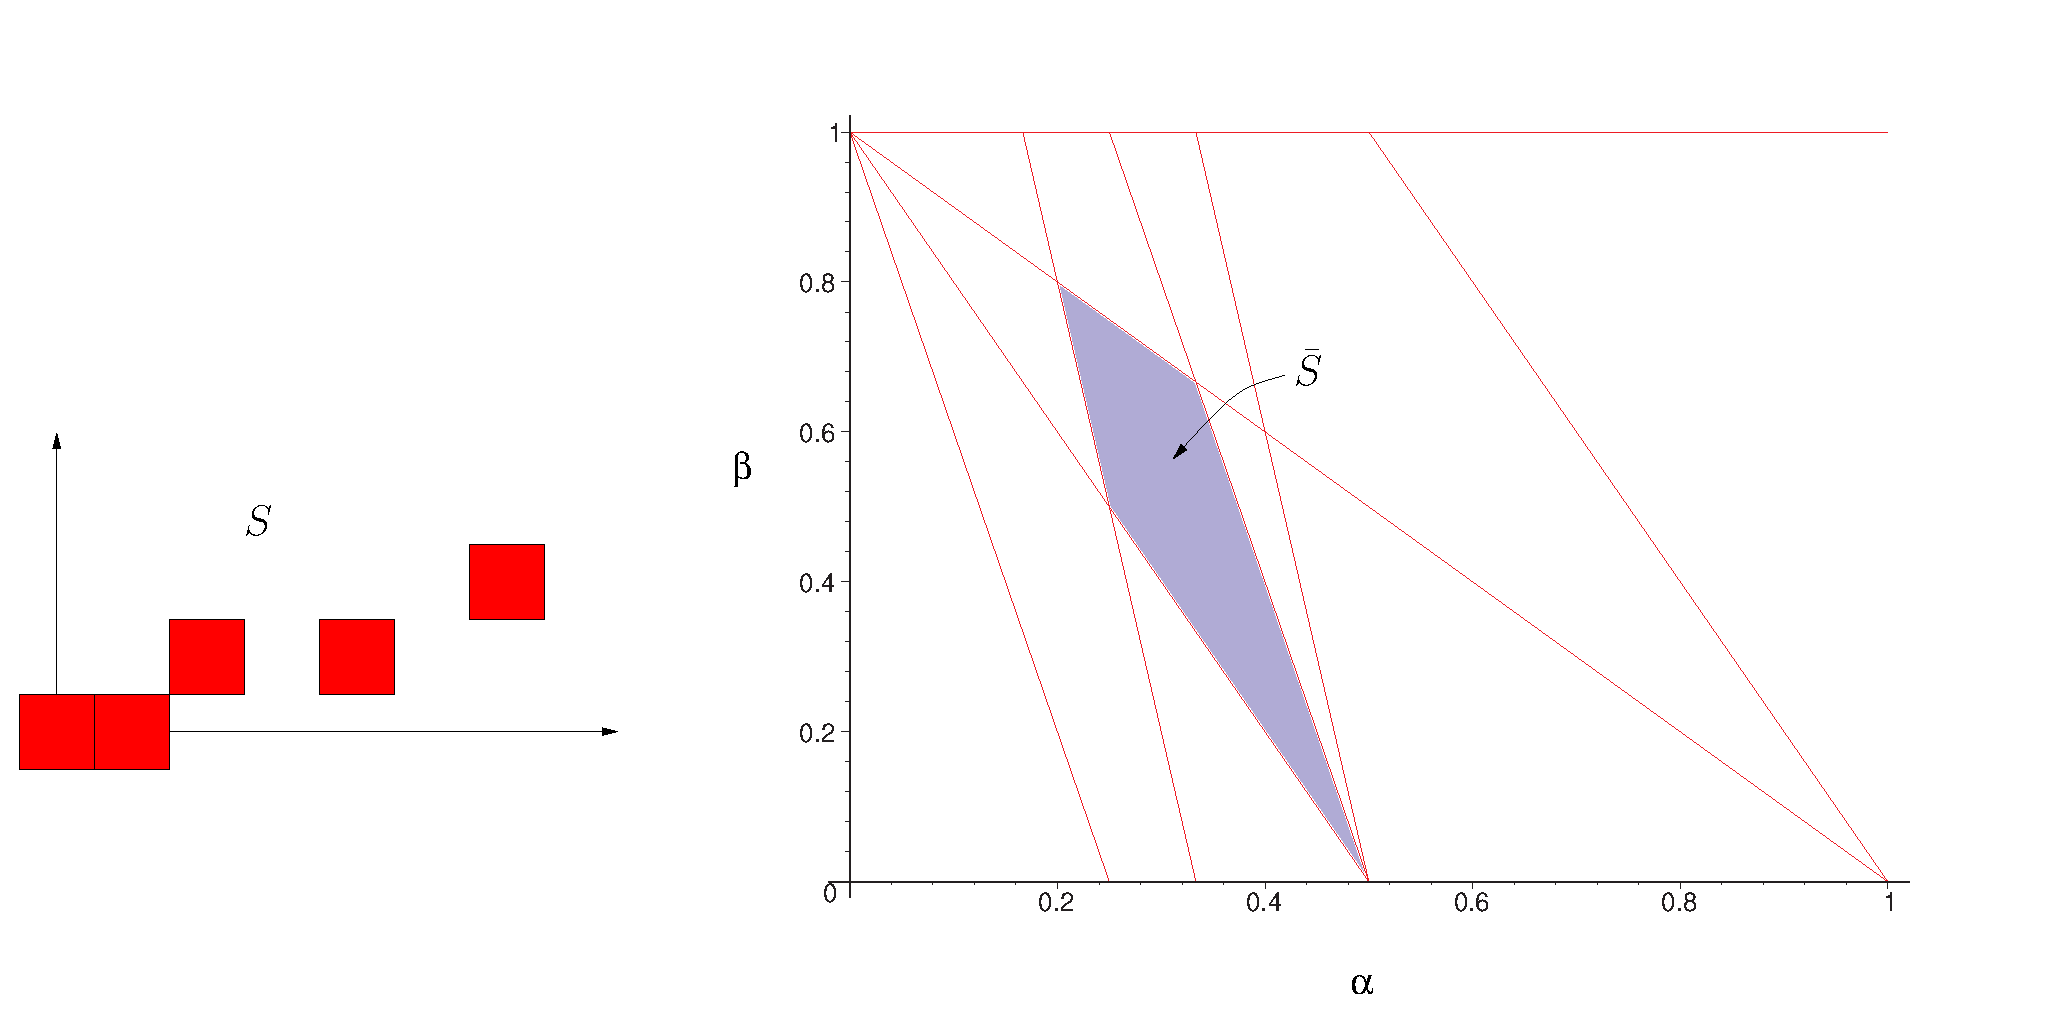
\includegraphics[width=10cm]{dual_exemplebis}
  \caption{Pr�image d'un ensemble de points discrets $S$.}
  \label{fig:preimage}
\end{figure}

\subsection{Plans et hyperplans discrets}

M�me si   la   litt�rature  est dense  sp�cifiquement  sur   les plans
discrets, nous allons  d�finir cet objet  dans  le m�me temps  que les
hyperplans discrets.  Trois  grandes d�finitions existent pour d�finir
cet objet g�om�trique dans $\Z^n$. Si ces trois d�finitions comportent
des similitudes et si elles sont parfois �quivalentes, les processus de
discr�tisation li�s � ces  d�finitions  peuvent varier.   Nous notons
$\Gamma$ un  hyperplan   euclidien  donn�  par  $\gamma_0+\sum_{i=1}^n
\gamma_ix_i=0$           avec             $\{\gamma_i\}\in\mathbb{R},~
|\gamma_i|\leq|\gamma_n|$ pour $1\leq  i < n$ et $|\gamma_n|>0$ (l'axe
$x_n$ est appel�  axe principal de l'hyperplan,  voir plus loin). Dans
les d�finitions suivantes, nous gardons les termes anglais pour �viter
toute ambigu�t�.

\begin{definition}[Digital hyperplane \cite{STO91}]
\label{def:digitalhp}
$S \subset \mathbb{Z}^n$  est un  \emph{digital  hyperplane} si et
seulement si il existe un hyperplan euclidien $\Gamma$ tel que $S$
soit l'\emph{image digitale} de $\Gamma$.
\end{definition}

La notion  \emph{d'image   digitale}  correspond �  un  processus   de
discr�tisation sp�cifique qui construit   les points discrets  dont la
distance verticale ($L_\infty$) sur  la $n-$i�me coordonn�e  entre le point discret
et le plan est inf�rieure � $\frac{1}{2}$.


\begin{definition}[Digital flatness \cite{veelaert_hyper}]
\label{def:flat}
$S\subset\mathbb{Z}^n$ est   {\em flat} si et seulement s'il existe
$n+1$ nombres r�els  $\gamma_0,\ldots,\gamma_n$ tels que~:
\begin{enumerate}
  \item $\max\{|\gamma_0|,\ldots,|\gamma_n|\}=1$\,;
  \item tout point $P=(P_1,\ldots,P_n)\in S$ v�rifie la condition
    \begin{equation}
      \label{eq:defflat}
      -\frac{1}{2}\ < \gamma_0 +\sum_{i=1}^n \gamma_iP_i \leq \frac{1}{2}\,.
    \end{equation}
\end{enumerate}
\end{definition}

Dans \cite{veelaert_hyper}  \aut{Veelaert}  montra qu'un \emph{digital
  hyperplan}  de  la d�finition  \ref{def:digitalhp} est  \emph{flat}.
Enfin nous avons  une d�finition � mettre en  parall�le avec la notion
de droite discr�te arithm�tique~:


\begin{definition}[Discrete analytic hyperplane \cite{bb36468}]
\label{def:analHP}
$S$ est un morceau de   \emph{discrete    analytic     hyperplane}    $P$   ayant pour
coefficients 
$(a_1,a_2,\ldots,a_n,b)\in           \mathbb{Z}^{n+1}$,
$pgcd(a_1,\ldots,a_n)=1$, et pour �paisseur $\omega\in\mathbb{N}^*$
si~:
  \begin{equation}
    \label{eq:defHP}
   S\subset P(a_1,a_2,\ldots,a_n,b)=\{(x_1,x_2,\ldots,x_n)\in\mathbb{Z}^n|0\leq b+\sum_{i=1}^n a_ix_i < \omega   \}
  \end{equation}
\end{definition}

Comme   pour   les  droites,  cette    d�finition   int�gre une notion
d'�paisseur.       Tout    comme       en      dimension     2,     si
$\omega=\max_{i=1..n}\{|a_i|\}$, elle d�finit un hyperplan discret
na�f  \cite{bb36468}.   Par la   suite,   c'est  cet objet  que   nous
consid�rerons dans les algorithmes de reconnaissance.

Si les coefficients  du plan  euclidien  $\Gamma$ dans  la  d�finition
\ref{def:digitalhp}     sont  rationnels,   alors  un    \emph{digital
  hyperplane} est aussi un \emph{digital analytic hyperplane}.

Nous concluons ces d�finitions par la notion d'axe principal et de
base d'un hyperplan discret.

\begin{lemme}[Axe principal et base d'un hyperplan discret]
  Soit $S$ un \emph{digital  hyperplane} ou un hyperplan discret na�f.
  Il existe alors un axe principal $x_j$ tel que la projection $S'$ de
  $S$ selon  l'axe  $x_j$ sur   le  plan $x_j=0$ soit   une bijection.
  L'ensemble  de points discrets de dimension  $(n-1)$ $S'$ est appel�
  la base de l'hyperplan.
\end{lemme}

Ce lemme est issu des  diff�rentes d�finitions et est g�n�ralis� dans
\cite{jamet_functionality}.       Par  exemple   pour    la d�finition
\ref{def:digitalhp}  l'axe principal   est $x_n$, dans   la d�finition
\ref{def:flat}, l'axe est  $x_j$  si $|\gamma_j|=1$.  Enfin, pour  les
hyperplans discrets na�fs, l'axe principal est $x_j$ si $\omega=|a_j|$
(voir figure \ref{fig:plandef}).

De   la m�me mani�re  que  pour  les droites  discr�tes, nous  pouvons
d�finir la pr�image comme �tant  l'ensemble des  hyperplans euclidiens
dont  le discr�tis� contient un ensemble  $S$ de points discrets. Nous
reviendrons dans la section \ref{sec:algor-de-reconn} sur cet objet.



\begin{figure}[h]
  \centering
  \subfigure[]{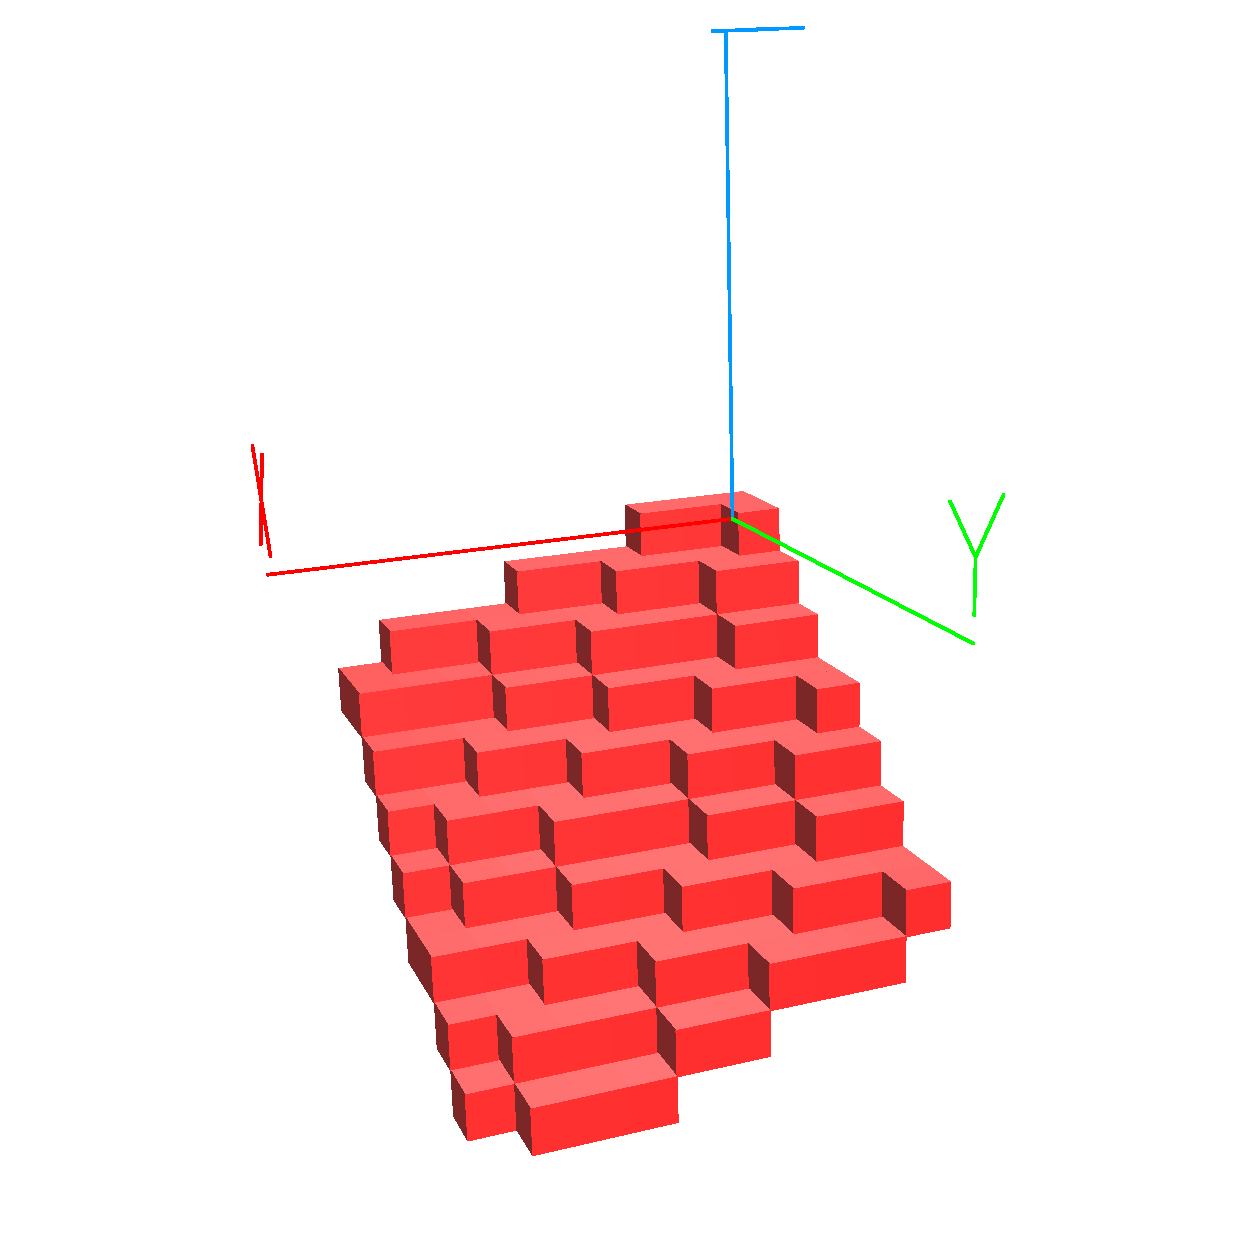
\includegraphics[width=6cm]{naif}}
  \subfigure[]{\includegraphics[width=3.5cm]{projection}}
  \caption{Morceau de plan discret na�f de param�tres $P(6,13,17,17)$
  $(a)$ et illustration de la base 2D associ� � un morceau de plan.}
  \label{fig:plandef}
\end{figure}


\subsection{Cercles, sph�res et hypersph�res discr�tes}

Toujours  en   fonction d'un   mod�le  de  discr�tisation,   plusieurs
d�finitions existent pour les cercles discrets ou  pour les sph�res et
hypersph�res.    Une d�finition  g�n�rale a  cependant �t�  donn�e par
\aut{Andr�s} et \aut{Jacob}~:

\begin{definition}[Hypersph�re discr�te analytique \cite{Andres_hypersphere}]
  \label{def:cercles-spheres}Une  hypersph�re discr�te  analytique  de dimension  $n$, de  centre
  $C\in\R^n$, de rayon $r\in\R$ et d'�paisseur  $\omega\in\R$ est l'ensemble des
  points discrets~:
  \begin{displaymath}
    H_n(C,r,\omega) = \left \{P\in\Z^n, \left (r-\frac{\omega}{2}\right)^2\leq
    \sum_{i=1}^n (C_i-P_i)^2 <\left (r+\frac{\omega}{2}\right)^2\right\}
  \end{displaymath}
\end{definition}

Dans \cite{Andres_hypersphere},  les  auteurs discutent   du param�tre
d'�paisseur en fonction   de  la connexit� souhait�e  pour  l'ensemble
discret  obtenu.  D'autres  r�sultats  de  connectivit�  ainsi  qu'une
formulation    analytique      du     cercle   de      \aut{Bresenham}
\cite{Bresenham_circular},  tr�s classique  en informatique graphique,
sont                         disponibles                          dans
\cite{FIORIO:2006:LIRMM-00128281:1,conf/dgci/FiorioT06}.  Dans le  cas
du  cercle de  \aut{Bresenham},  si une telle caract�risation  existe,
elle met en place une �paisseur non constante et ne rentre donc pas
enti�rement dans le cadre de la d�finition \ref{def:cercles-spheres}.

De cette d�finition analytique,  nous retenons dans les algorithmes de
reconnaissance  de  la  section \ref{sec:algor-de-reconn} le  principe
suivant (pour la dimension 2)~: un ensemble $S$ de points discrets est
un   disque discret   s'il existe  un  cercle  s�parant    $S$ de  son
compl�mentaire $\bar{S}$. Nous nous  ram�nerons ainsi � un probl�me de
s�parabilit�.



\section{La bo�te � outils}

Dans  ces paragraphes, nous pr�sentons  diff�rents  outils de domaines
vari�s permettant d'offrir des solutions algorithmiques efficaces � la
reconnaissance des objets �l�mentaires.

\subsection{Programmation lin�aire}
\label{sec:progr-line}

Un probl�me de  programmation par contrainte consiste �  maximiser une
fonction objectif lin�aire �tant   donn�  un ensemble  de  contraintes
lin�aires. Le syst�me de contraintes peut se d�finir de mani�re
g�n�rale par~:

\begin{displaymath}
  \left \lbrace
    \begin{array}{c}
      a_{11} x_1 + a_{12} x_2 +\ldots +a_{1n} x_n \leq b_1\\
      a_{21} x_1 + a_{22} x_2 +\ldots +a_{2n} x_n \leq b_2\\
      \ldots\\
      a_{m1} x_1 + a_{m2} x_2 +\ldots +a_{mn} x_n \leq b_m\\

    \end{array}\right.
\end{displaymath}
ou plus simplement par une repr�sentation matricielle~:
\begin{displaymath}
Ax\leq b
\end{displaymath}
avec        $A=(a_{ij})\in\mathbb{R}^{m\times        n}$            et
$b=(b_i)\in\mathbb{R}^m$. La  fonction objectif  est donn�e de mani�re
g�n�rale sous la forme $cx$ avec $c=(c_j)\in\mathbb{R}^n$.


On cherche donc � r�soudre~:
\begin{align*}
  &\max cx\\
  & Ax\leq b\\
  & x\in\R^n
\end{align*}

De nombreux algorithmes existent pour r�soudre ce syst�me (not� LP)
\cite{schrijver86}. D'un point de vue th�orique, nous avons le
r�sultat suivant~:

\begin{theoreme}[\cite{Megiddo84}]
  �tant donn� un probl�me LP donn� avec  $m$ contraintes lin�aires dans $\mathbb{R}^n$
  o�  $n$ est fixe, il existe alors un algorithme permettant de
  r�soudre le probl�me en  $O(m)$.
\end{theoreme}

Si ce r�sultat est tr�s fort d'un point de vue th�orique, l'algorithme
sugg�r� par   \aut{Megiddo} n'est impl�mentable  que  pour  de faibles
dimensions (2, voire 3).  Notons aussi  que la constante dans la borne
lin�aire est  tr�s grande (doublement  exponentielle en la dimension).
En pratique, on pr�f�re utiliser des techniques parfois exponentielles
en temps (comme le \texttt{Simplex}) mais  tr�s rapides en pratique, ou
encore    des    approches      \emph{randomis�es}   (voir    par     exemple
\cite{goldwasser95survey}).


\subsection{Programmation lin�aire enti�re}

Un probl�me de programmation lin�aire enti�re est un probl�me lin�aire
dans lequel les contraintes  sont donn�es par des coefficients entiers
et  dont on  cherche  des  solutions enti�res \cite{schrijver86}.   Le
probl�me s'�crit donc~:
\begin{align*}
  &\max{cx}\\
 & Ax\leq b\label{syst}\\
& x\in \mathbb{Z}^n
\end{align*}
sachant             $A=(a_{ij})\in\mathbb{Z}^{m\times             n}$,
$b=(b_i)\in\mathbb{Z}^m$ et $c=(c_j)\in\mathbb{Z}^n$.

D�cider si une solution  $x\in\Z^n$ existe est un probl�me  NP-complet
\cite{GareyJohnson}.   Cependant,     de   nombreux  travaux  visent �
caract�riser   cet     ensemble  de    point  discret     s'il  existe
\cite{schrijver86,BarHowLov92,zolo,Barany02}.

Le syst�me de contraintes $A$ et $b$ d�finit un polytope $\mathcal{P}$
de $\R^n$  qui correspond au domaine dans  lequel il faut chercher les
points discrets  solutions.  Consid�rons  $P$  l'enveloppe convexe  de
$\mathcal{P}\cap\mathbb{Z}^n$.   C'est  ce  polytope discret que  nous
allons caract�riser. On note $N(A,b)$ l'ensemble des sommets de $P$ et
nous nous int�ressons � $|N(A,b)|$.

\begin{theoreme}[\cite{zolo}]
\label{theo:zolo}
Soient                $A=(a_{ij})\in\mathbb{Z}^{m\times           n}$,
$b=(b_i)\in\mathbb{Z}^m$,            $c=(c_j)\in\mathbb{Z}^n$       et
$\alpha=\max\{|a_{ij}|, i=1,\ldots,m,j=1,\ldots,n\}$. Nous avons,
  \begin{equation}
|N(A,b)| \leq  c_n m^{\lfloor n/2\rfloor}\log^{n-1}(1+\alpha)\,
  \end{equation}
  o� $c_n$ est une quantit� d�pendant uniquement de la dimension $n$.
\end{theoreme}

Ce r�sultat nous servira �  borner l'enveloppe convexe d'un morceau de
plan   discret    et      de   sa  pr�image       dans    la   section
\ref{sec:reco-plans-et-hyperplans}.

\begin{figure}[ht]
  \centering
  \subfigure[]{\includegraphics[width=3.5cm]{acketa}}
  \subfigure[]{\includegraphics[width=5cm]{exempleILP}}
  \subfigure[]{\includegraphics[width=5cm]{exempleILPcvx}}
  \caption{$(a)$ Exemple   de  polygone convexe   discret inclus.  Les
    figures $(b)$ et $(c)$  illustrent  la combinatoire entre  l'objet
    discret (ici 3D) et les sommets de son enveloppe convexe $(c)$.}
  \label{fig:acketa}
\end{figure}

\subsection{Polytopes discrets}

Dans la  section pr�c�dente, nous avons  d�j� pr�sent� des r�sultats
sur les polytopes discrets lorsque ceux-ci sont d�finis comme l'espace
des  solutions  d'un    probl�me  de programmation  lin�aire    enti�re.
Ci-dessous,   nous caract�risons le nombre  de   sommets d'un polytope
discret si  celui-ci  est donn�  par  la discr�tisation  (au  sens  de
\Name{Gauss}) d'un polytope continu ayant certaines propri�t�s.

Soit  $P$ un polytope discret de   dimension $n$ non-vide. Nous notons
$f_k(P)$ le nombre de facettes de dimension $k$  de $P$ ($0\leq k <n$,
par exemple $f_0$ est le nombre de sommets de $P$). Nous avons alors
le r�sultat suivant~:
\begin{theoreme}[\cite{BaranyLarman}]
  \label{theo:vol}
  \begin{equation}
    f_k\leq c_n (\text{Vol}~ P)^{\frac{n-1}{n+1}}\,
  \end{equation}
  o� $c_n$ ne   d�pend que de  la  dimension $n$ et  (Vol  $P$) est le
  volume de $P$.
\end{theoreme}


En  dimension    2,  ce    r�sultat    est �quivalent �   un  r�sultat
d'\aut{Acketa} et \aut{{\v{Z}}uni{\'c}} qui permet de borner le nombre
d'ar�tes $e(N)$ d'un polygone convexe discret contenu dans une fen�tre
$N\times N$ \cite{balog,acketa}~:
\begin{equation}
\label{eq:acketa}
  e(N)= \frac{12}{(4\pi^2)^{1/3}}N^{2/3}+O(N^{1/3}log(N))\,.
%% *** HERE WE NEED ANOTHER BOUND (OF BARANY-LARMAN, I'LL PUT IT)
\end{equation}

Le th�or�me \ref{theo:vol}   peut m�me �tre g�n�ralis� en  consid�rant
non   plus  un   polytope  discret $P$,   mais  la   discr�tisation de
\Name{Gauss} d'une forme continue ayant certaines propri�t�s~:

\begin{theoreme}[\cite{BaranyLarman}]
\label{BaranyLarman}
Soit $K \in C(D)$ o� $C(D)$ est la famille des formes convexes ayant un
bord $C^2$ et ayant un rayon de courbure en tout  point et dans toutes
les directions entre $1/D$ et  $D$, pour $D  \geq 1$.   Notons $\bar K  =
conv(K \cap \mathbb{Z}^n)$. Si le diam�tre $\delta$ de $K$ est suffisamment
grand, alors pour tout  $n  \geq 2$, il existe deux constantes
$c_1(n)$ et  $c_2(n)$ telles que pour tout  $k \in \{ 0,1, \dots, n-1 \}$,
%---------------
\begin{equation}
\label{barany}
c_n \delta^{n \frac{n-1}{n+1}} \leq f_k(\bar K) \leq c'_n \delta^{n \frac{n-1}{n+1}}.
\end{equation} 
%-------------
\end{theoreme}
%----------

Ces r�sultats  sont fondamentaux   pour  de  nombreux aspects  de   la
reconnaissance de formes discr�tes �l�mentaires. C'est le cas pour les
plans discrets ou les cercles discrets. Ils sont de plus � la base de
diff�rentes   preuves    de  convergence  asymptotique   d'estimateurs
g�om�triques comme la longueur ou les normales de contours discrets 2D
\cite{deVieilleville_these}.


\subsection{Enveloppe convexe}

A  de   nombreux    endroits     des algorithmes   de      la  section
\ref{sec:algor-de-reconn},  ces derniers n�cessitent des constructions
d'enveloppes  convexes \cite{P16,boissonnat,dcg-handbook}.   Dans   le
tableau    \ref{tab:cvx},  nous    reprenons  quelques    r�sultats de
complexit�.  Dans ce  tableau, $m$   correspond  au nombre  de  points
consid�r�s, $n$  la  dimension  et $h$  la taille   du r�sultat.   Les
algorithmes  incorporant  cette  quantit�  $h$  dans   leur mesure  de
complexit� sont dits \emph{output sensitive}, c'est-�-dire que le co�t
est  li� � la taille du  r�sultat.   Les algorithmes incr�mentaux nous
permettent  d'ins�rer les  points  un �  un  et  de maintenir � chaque
instant  une  enveloppe convexe  des points trait�s.   On peut vouloir
quantifier    le  co�t  algorithmique de  l'ajout     d'un point.  Par
algorithme dynamique, nous  entendons  un algorithme dans lequel  nous
pouvons ajouter et supprimer des points.

Nous  avons aussi  ajout�  au tableau deux  r�sultats  dans le cas  o�
l'ensemble de points en entr�e est � support discret.  Dans ce cas, le
calcul d'enveloppe  convexe d'une courbe discr�te  est lin�aire en son
nombre de points \cite{voss}. Notons que si la courbe discr�te est vue
comme  une  cha�ne,    les r�sultats  de   \cite{IPL::Melkman1987}  ou
\cite{buzer_cvxhull}   peuvent  aussi �tre utilis�s.  L'algorithme  de
\aut{Har-Peled} \cite{har-peled98} est  cependant � mettre en  avant~:
cet algorithme est \emph{output sensitive} et son co�t est ind�pendant
(dans  une  certaine  mesure)  de   la cardinalit� de  $X$,  d�pendant
seulement  de son  diam�tre $\delta(X)$.    Notons  cependant que  les
hypoth�ses sur  la  classe d'objets  $X$  permettant d'atteindre cette
borne sont fortes. 


\begin{table}[h]
  \centering
  \begin{tabular}{|l|c|r|}
    \hline
    Objets & Complexit� au pire cas& R�f�rences\\
\hline
\hline
    Points 2D & $O(m \log m)$ & \aut{Graham} \cite{Graham:72}\\
    Points 2D & $O(m h)$ & \aut{Jarvis} \cite{jarvis73}\\
    Points 2D & $O(m \log h)$ & \aut{Chan} \cite{citeulike_937376}\\
    Points 3D & $O(m\log h)$ & \aut{Chan} \cite{citeulike_937376}\\
    Points dD & $O(m\log m + m^{\lfloor n/2\rfloor})$ & \aut{Chazelle}
    \cite{journals/dcg/Chazelle93}\\
    \hline
    \hline
    Cha�ne simple 2D & $O(m)$ incr�mental $O(1)$ & \aut{Melkman} \cite{IPL::Melkman1987}\\
    Cha�ne simple 2D & $O(m)$ dynamique $O(1)$ &\aut{Buzer} \cite{buzer_cvxhull} \\
    \hline
    \hline
    Courbe discr�te & $O(m)$  & \aut{Voss} \cite{voss}\\
    Objet discret convexe $X$& $O(h\log{\delta(X)})$& \aut{Har-Peled} \cite{har-peled98}\\

\hline
  \end{tabular}
  \caption{Enveloppes convexes et principales r�f�rences.}
  \label{tab:cvx}
\end{table}


\subsection{S�parabilit� par cercles}

Pour terminer avec les outils dont nous aurons besoin, nous pr�sentons
quelques  r�sultats  concernant  le  probl�me  de  s�paration  de deux
ensembles par des cercles en g�om�trie algorithmique.

Le probl�me peut-�tre expos�  de la fa�on suivante~: �tant donn�s deux
ensembles $S$ et $T$, comment  d�cider s'il existe un cercle contenant
tous les points de $S$ et ne contenant aucun  point de $T$ ? Autrement
dit, est-ce que $S$ et $T$ sont s�parables par un cercle ?

Si nous  notons $m=|S|+|T|$, \aut{O'Rourke} \etal \cite{ORourke:1986a}
ont propos�  une  r��criture du probl�me  en   termes de programmation
lin�aire en dimension 3 de $m$ contraintes. En utilisant les r�sultats
de  \aut{Megiddo} (voir  section  \ref{sec:progr-line}), nous obtenons
les r�sultats pr�sent�s  dans le tableau  \ref{tab:sep}. Notons que si
d'un point de  vue th�orique, la  r�solution d'un probl�me lin�aire en
dimension 3 est lin�aire au nombre de contraintes, l'impl�mentation de
cet algorithme est tr�s complexe.

Si nous nous restreignons �  des outils en  dimension 2, nous  pouvons
consid�rer  un test de s�parabilit� bas�  sur une notion de cellule de
\aut{Vorono�} g�n�ralis�e  construite en  consid�rant tous les couples
$(s,t)$ avec $s\in S$ et $t\in T$ \cite{dcoeurjo_digitalarc_DAM}. Nous
obtenons ainsi  des co�ts  sup�rieurs   mais l'impl�mentation  de  ces
algorithmes est r�alisable (voir tableau \ref{tab:sep}).

\begin{table}[h]
  \centering
  \begin{tabular}{|p{6.5cm}|p{3cm}|r|}
    \hline
    Caract�ristique & Compl�xit� au pire cas& R�f�rences\\
\hline
\hline
    Test de s�parabilit� (LP dimension 3)& $O(m)$ &  \cite{ORourke:1986a}\\
    Extraction du cercle s�parant de rayon minimal & $O(m)$ &
    \cite{ORourke:1986a}\\
    Extraction de tous les cercles s�parants & $O(m\log m)$&
    \cite{ORourke:1986a}\\
    \hline
    \hline
    Test s�parabilit� (LP dimension 2) & $O(|S|\cdot|T|)$ & \cite{P16,dcoeurjo_digitalarc_DAM}\\
    Extraction de tous les cercles s�parants &
    $O(|S|\cdot|T|\log(|S|\cdot|T|))$ incr�mental&
    \cite{P16,dcoeurjo_digitalarc_DAM}\\
    \hline
  \end{tabular}
  \caption{Principales r�f�rences pour la s�parabilit� de deux
    ensembles par un cercle.}
  \label{tab:sep}
\end{table}

\section{Algorithmes de reconnaissance}
\label{sec:algor-de-reconn}

Nous   allons maintenant  combiner   tous les  outils  pr�c�dents pour
synth�tiser  les   diff�rentes   approches pour   la    conception des
algorithmes  de   reconnaissance  et     pour pr�senter    leur   co�t
algorithmique.

Quel  que  soit   l'objet �l�mentaire  reconnu et �tant  donn�   qu'il
existera toujours  un   nombre  infini  de repr�sentants    euclidiens
associ�s � un ensemble fini  de points discrets, deux grandes  classes
d'algorithmes  peuvent �tre d�finies~:    la  premi�re contient    les
algorithmes de d�tection qui ont soit une  r�ponse binaire au probl�me
de d�cision associ�, soit retournent un unique repr�sentant euclidien.
La seconde   classe reprend les  algorithmes bas�s  sur une  notion de
pr�image nous   retourneront    toutes les    solutions  sous    forme
g�n�ralement d'un polytope dans un certain espace des param�tres.




\subsection{Droites discr�tes}


Concernant les  algorithmes de reconnaissance   de droite discr�te, le
probl�me      a �t�  tr�s �tudi� et  des   solutions
efficaces  existent.    Le tableau    \ref{tab:reco_droite} synth�tise
quelques-unes de ces solutions. Rappelons que les param�tres issus des
algorithmes de   reconnaissance    dits   ``arithm�tiques''  d�crivent
compl�tement la pr�image associ�e aux droites discr�tes.

D'un   point de vue pratique,  les  algorithmes de reconnaissance sont
assez simples et ne n�cessitent pas d'outils tr�s complexes.


\begin{table}[h]
  \centering
  \begin{tabular}{|p{2.5cm}|l|c|r|}
    \hline
    Contrainte & Caract�ristique &  Complexit� au pire cas& R�f�rences\\
    \hline
    \hline
    Courbe connexe& Calcul de bande minimale & $O(m)$ incr�mental $O(1)$&    \cite{KOV_1990}\\
\cline{2-4}&    Reco. arithm�tique & $O(m)$ incr�mental $O(1)$
    &    \cite{DEB95,debled}\\
\cline{2-4} &Reco. arithm�tique & $O(m)$ dynamique $O(1)$ &    \cite{deVieilleville_these}\\
    \cline{2-4} &Pr�image & $O(m)$ incr�mental $O(1)$ & \cite{dor91,bruck93}\\
    \hline\hline

    Non connexe mais avec ordre & Pr�image & $O(m)$ incr�mental & \cite{rourke}\\
    \hline
    \hline
    Non connexe & Test lin�arit� LP dimension 2 & $O(m)$ incr�mental &
    \cite{megiddo_LP,bb16862}\\
    \cline{2-4}
    & Preimage LP dimension 2 & $O(m \log m)$ incr�mental& \cite{P16}\\
\hline 
  \end{tabular}
  \caption{Algorithmes de reconnaissance de droite discr�te.}
  \label{tab:reco_droite}
\end{table}



\subsection{Plans et hyperplans discrets}
\label{sec:reco-plans-et-hyperplans}


Concernant les plans et  hyperplans discrets, les probl�mes sont  plus
complexes. Intuitivement, nous  avons peu d'algorithmes exploitant les
propri�t�s arithm�tiques et  de p�riodicit�s des plans discrets  comme
c'�tait le  cas en dimension 2. Cependant,   nous avons des techniques
fond�es sur des outils classiques de  g�om�trie algorithmique mais dont
les complexit�s sont modul�es par  le caract�re discret des objets  en
exploitant la combinatoire sp�cifique des polytopes discrets.

Pour la construction  des  algorithmes de reconnaissance,  nous allons
utiliser  diff�rents   r�sultats.     Tout  d'abord,   nous   appelons
\emph{support} d'un  ensemble   de  points dans   $\R^n$ un  hyperplan
euclidien tel que tous  les points de  l'ensemble sont du m�me c�t� de
l'hyperplan.   On  note   aussi     $L_\infty$  la  distance   infinie
($L_\infty(p,q)=\max_i{|p_i-q_i|}$). Ainsi~:

\begin{theoreme}[\cite{Kim84f}]
\label{theo:kim}
Soit  $S \subset \mathbb{Z}^3$. $S$ est  un morceau de  plan discret si et
seulement s'il  existe  un plan    support  $H$ de    $S$ tel que   la
$L_\infty$-distance entre tout point  de $S$ et $H$  soit inf�rieure �
1.
\end{theoreme}

�nonc� pour la dimension 3, ce th�or�me est g�n�ralisable en dimension
sup�rieure car li� � la d�finition m�me  des hyperplans discrets. D'un
point de  vue algorithmique, il  est clair que  la  recherche d'un tel
plan support   peut �tre  effectu�e   en s'int�ressant �   l'enveloppe
convexe $CH(S)$ de   $S$.  Notons  que dans \cite{Kim84f,kim91}    les
auteurs   proposent un  algorithme   de  recherche  de  $H$  en  temps
quadratique (voir tableau \ref{tab:survey})  mais ce dernier n'est pas
correct  dans  certains  cas  \cite{debled}.   Toujours   dans ce
contexte, nous avons le r�sultat suivant~:

\begin{theoreme}[\cite{STO91}]
\label{theo:stoj}
Soit  $S \subset  \mathbb{Z}^n$.  $S$    est un moreceau   d'hyperplan
discret si et   seulement s'il  existe   un hyperplan euclidien   $H$
s�parant  $S$ et $S'$,  $S'$ �tant obtenu par translation  de $S$ de 1
selon l'axe principal de $H$.
\end{theoreme}

L� encore, le test de s�paration de $S$ et de $S'$ peut �tre r�solu en
regardant si   $CH(S)\cap  CH(S')$   est   vide  ou  non.  Notons  que
\cite{STO91} pr�sente un test de s�parabilit� bas� sur la construction
d'un probl�me de programmation lin�aire en dimension 3.  Pour terminer
avec  ces  caract�risations g�om�triques, nous consid�rons l'�paisseur
g�om�trique de $S$ comme �tant l'intersection entre l'axe principal de
$S$ et l'enveloppe     convexe  de l'ensemble  corde    associ� �  $S$
\cite{GerDebZim05}.  L'ensemble corde  est donn� par  $\{P-P', \forall
P,P'\in S\}$. Ainsi nous avons~:
\begin{theoreme}[\cite{GerDebZim05}]
  Soit $S \subset  \mathbb{Z}^3$.  $S$ est un  morceau de plan discret
  si et seulement si son �paisseur g�om�trique est inf�rieure � 1.
\end{theoreme}

Pour les  trois approches pr�c�dentes,  la combinatoire de l'enveloppe
convexe  d'un  ensemble de points discrets   est un �l�ment crucial dans
l'analyse de  complexit� ou tout du   moins dans l'efficacit� pratique
des  algorithmes.  La   figure  \ref{fig:CG} illustre ces  diff�rentes
approches g�om�triques.


\begin{figure}[ht]
  \centering
  \includegraphics[width=12cm]{CG}
  \caption{Illustration     des     approches g�om�triques   pour   la
    reconnaissance d'hyperplans   discrets~: l'ensemble   $S$ initial,
    calcul d'un plan support,  test de s�parabilit� $S$/$S'$ et calcul
    de l'�paisseur g�om�trique de l'ensemble corde de $S$.}
  \label{fig:CG}
\end{figure}


A c�t� de ces approches, nous avons aussi toutes les techniques issues
de     la programmation lin�aire.   En    effet,   avec la  d�finition
\ref{def:flat} (resp.  la  d�finition  \ref{def:analHP}), nous pouvons
associ� � chaque point discret $P$ de $S$  deux contraintes avec $n+1$
inconnues    $\{\gamma_0,\ldots,\gamma_n\}$ dans $\R^{n+1}$     (resp.
$\{a_1,\ldots,a_n,b\}$  dans $\mathbb{Z}^{n+1}$).   Nous avons   ainsi
deux probl�mes LP  et LP enti�re pour   d�cider si $S$  est un morceau
d'hyperplan  discret  ou  non.  Si  nous   consid�rons une orientation
sp�cifique pour   l'hyperplan recherch�, c'est-�-dire si   nous fixons
l'axe principal,   nous  pouvons nous   ramener � un   probl�me LP  en
dimension    $n$         en         consid�rant    les     inconnues~:
$\{\gamma_0/\gamma_n,\ldots,\gamma_{n-1}/\gamma_n,1\}$              ou
$\{a_1/a_n,\ldots,a_{n-1}/a_n,1,b/a_n\}$ car alors $\gamma_n\neq 0$ et
$a_n\neq 0$. Le probl�me de  LP enti�re devient maintenant un probl�me
LP  sur $\mathbb{Q}$.   Nous   pouvons  donc associer �   chaque point
discret  $P\in S$  dans un espace   des param�tres $\{\Gamma_0,\ldots,
\Gamma_{n-1}\}\in\R^{n-1}$, les contraintes~:
\begin{equation}
  \Gamma_0-\frac{1}{2}+P_n+\sum_{i=1}^{n-1}        \Gamma_iP_i    \leq
0 \quad\text{et}\quad \Gamma_0+\frac{1}{2}+P_n+\sum_{i=1}^{n-1}        \Gamma_iP_i    >
0\label{eq:constraints}\,.
\end{equation}

Nous pouvons      alors  reprendre  les r�sultats    de     la section
\ref{sec:progr-line} pour r�soudre ce probl�me et ainsi d�cider si $S$
est un  morceau  d'hyperplan  discret.   Par exemple,  le  r�sultat de
\aut{Megiddo} nous dit que si la dimension est fixe, la reconnaissance
d'hyperplan discret  est calculable en  temps lin�aire  par rapport au
nombre de points discrets.

Dans des dimensions faibles, nous pouvons nous int�resser au calcul de
la pr�image compl�te. Pour les dimensions sup�rieures, la combinatoire
de   la  pr�image (polytope  de  $\R^n$)  ne  permet pas   d'avoir des
algorithmes    de  mise � jour  de    celle-ci   qui soient  efficaces
\cite{boissonnat}.

Pour  les plans  discrets,  la pr�image   est un  objet  tr�s utilis�e
\cite{vittonethese,vittone,veelaert_hyper,dcoeurjo_these,sivignon_these,dexet_these}.
L'un des principal int�r�ts �tant que la pr�image d�crit l'infinit� des
plans euclidiens  associ�s � un morceau   de plan  discret.  Or  cette
description est primordiale lorsque l'on s'int�resse au probl�me de la
reconstruction r�versible (voir chapitre   \ref{chap:reconstruction}).
Dans  la suite, on  note $\P(S)$ la  pr�image associ�e � l'ensemble de
points discrets $S$.

L'algorithme est    tr�s simple, nous  faisons  l'hypoth�se  que l'axe
principal du plan est l'axe $x_3$  (axe $Oz$).  Ensuite, sans perte de
g�n�ralit�, nous initialisons la pr�image dans l'espace des param�tres
$(\Gamma_0,\Gamma_1,\Gamma_2)$        (notation      de      l'�quation
(\ref{eq:constraints}))  par le  cube  $[0,1]^3$.  Pour  chaque  point
discret $P\in S$, nous allons mettre � jour  la pr�image avec les deux
contraintes associ�es (Equ. (\ref{eq:constraints})). Plus pr�cis�ment,
nous avons deux  calculs d'intersection entre  un poly�dre convexe, et
une contrainte lin�aire.     Pour  cette mise � jour,   nous   pouvons
utiliser un  algorithme lin�aire en  la taille de  la pr�image dans le
pire  cas.  Si au cours  de  l'algorithme  $\P(S)$ devient vide,  cela
signifie qu'il  n'existe  aucun plan euclidien  dont la discr�tisation
contienne $S$. Nous  concluons alors que $S$  n'est  pas un  morceau de
plan discret.

Cet algorithme incr�mental a donc un co�t  en $O(m\cdot E)$ o� $m=|S|$
et  $E$ est  le  nombre d'ar�tes de  la  pr�image.   Un point  crucial
consiste donc � donner une borne sur  la quantit� $E$. Nous aborderons
ce point  dans  la section  suivante.   S'il est   difficile de parler
d'algorithme \emph{output sensitive} pour un algorithme incr�mental, �
chaque �tape, nous avons un processus qui est lin�aire en la taille de
la sortie de l'�tape pr�c�dente.



Le tableau   \ref{tab:survey} reprend les  diff�rentes approches. Pour
plus  de pr�cisions sur   des  algorithmes  non  d�taill�s  ci-dessus,
se r�f�rer � \cite{dcoeurjo_iwcia2006}.

\begin{table}[ht]
  \centering
  \begin{tabular}{|p{5cm}|c|p{1cm}|p{2.5cm}|p{1.5cm}|}
    \hline
    Description & Ref. & Dim. &  Complexit�& Incr�mental \\
    \hline
    Caclul plan support avec distance < 1 & \cite{Kim84f,kim91}& 3 & $O(m^2)$ & - \\
    S�parabilit�  bas�e sur l'enveloppe convexe & \cite{STO91} & n 
    &$O(m\cdot\log{m}+m^{\lfloor n/2\rfloor} + 2^n\cdot m^{2^{n-2}n}\cdot\log{m})$ & -  \\
    �paisseur de $S$ & \cite{GerDebZim05} & 3 & $O(m^7)$ & oui\\
    \hline
    \hline
    Algorithme \aut{Fourier-Motzkin} & \cite{fourier} & 3 & n.a. &-  \\
    LP & \cite{Megiddo84} & n fixe &    $O(m)$& - \\
    S�parabilit� bas�e sur LP & \cite{STO91} &  n fixe &    $O(m)$& - \\

    LP enti�re & \cite{conf/dgci/BrimkovD05} & n fixe & $O(m\cdot\log{D})$ & - \\
    Pr�image arithm�tique& \cite{vittone} & 3 &$O(mE^2\cdot\log{D})$ & oui   \\
    Pr�image arithm�tique& \cite{dcoeurjo_these}  & 3 &$O(m\cdot\log^2{m})$ & oui    \\
    Pr�image &  & 3   & $O(m\cdot E)$ & oui  \\
    \hline
    \hline
    Propri�t� \emph{Evenness} (base rectangulaire) & \cite{veelaert} & 3 & $O(m^2)$&oui \\

    \hline
    \hline
    Reconnaissance arithm�tique  (base rectangulaire) & \cite{mesmoudi} &3 & & -  \\
    \hline
  \end{tabular}
  \caption{Solutions algorithmiques pour la reconnaissance de plans et
    d'hyperplans discrets~: $m$ est le nombre de points discrets, $n$
    la dimension, $E$ est la taille de la pr�image, et $D$ une borne
    sur la taille du domaine contenant l'ensemble $S$.}
  \label{tab:survey}
\end{table}


M�me   si   l'algorithme   de    \aut{G�rard}   \etal
\cite{GerDebZim05}   poss�de une  borne au  pire   cas tr�s importante
($O(m^7)$),  ce dernier est lin�aire  en  pratique.  Ce point renforce
l'id�e que la structure  particuli�re  des morceaux de plans  discrets
joue un r�le  crucial dans l'efficacit�  des algorithmes.  C'est cette
sp�cificit� discr�te que nous analysons dans la section suivante.

\subsection{Pr�image et enveloppe convexe d'un hyperplan discret}

Nous  cherchons ici � �valuer la  combinatoire  associ�e � l'enveloppe
convexe de morceaux d'hyperplans discrets et ce pour deux raisons
fondamentales~:
\begin{itemize}
\item l'enveloppe convexe intervient � de nombreuses reprises dans les
  algorithmes de reconnaissance bas�s sur la g�om�trie~;
\item   dans   \cite{dcoeurjo_these,dcoeurjo_preimage_DAM}, nous avons
  montr� qu'en dimension 3, $|\P(S)| \leq |CH(S)|$.
\end{itemize}

Commen�ons  par �valuer   ces quantit�s en   utilisant des g�n�rateurs
al�atoires de plans et hyperplans discrets. Pour �valuer $CH(S)$, nous
utilisons      les        outils           de       la        libraire
\texttt{qhull}\footnote{\url{http://www.qhull.org/}}.  Pour g�n�rer un
hyperplan discret, nous commen�ons par  g�n�rer  sa base (ensemble  de
points discrets  dans  $\Z^{n-1}$),  nous  g�n�rons al�atoirement   un
vecteur normal que nous utilisons pour \emph{relever} la base et ainsi
construire   l'hyperplan dans   $\Z^n$.     Dans ce  qui   suit,  nous
consid�rons   des  morceaux connexes contenus   dans  un domaine born�
$N^n$.  Deux g�n�rateurs  pour  la base  seront utilis�s (voir  figure
\ref{fig:random})~:
\begin{itemize}
\item  base  hyper-rectangulaire~: on construit  un hyper-rectangle de
  dimension $n-1$ dont les  longueurs des diff�rents c�t�s  sont tir�s
  al�atoirement~;
\item base  ``co-sph�rique''~:   on utilise un   g�n�rateur  de points
  co-sph�rique dans  $\R^{n-1}$    fourni avec  \texttt{qhull},   nous
  utilisons   ensuite  \texttt{qhull}   pour en  calculer  l'enveloppe
  convexe  et ainsi construire   une   base discr�te comme �tant    la
  discr�tisation de ce convexe.
\end{itemize}

Le dernier g�n�rateur aura pour  objectif de tester des hypoth�ses pour
la classe des morceaux d'hyperplans discrets � base convexe.


\begin{figure}[h]

 \begin{center}
   \subfigure[]{ \includegraphics[width=4cm]{vox30}}
   \subfigure[]{ \includegraphics[width=4cm]{cvx30}}
   \subfigure[]{ \includegraphics[width=4cm]{preim30}}

    \subfigure[]{\includegraphics[width=4cm]{examplerounded}}
    \subfigure[]{\includegraphics[width=4cm]{examplerounded_cvx}}
   \subfigure[]{\includegraphics[width=4cm]{examplerounded_preim}}
  \end{center}
  \caption{Illustration de  deux morceaux de  plans discrets selon les
    g�n�rateurs  propos�s~:    $(a)$  un  morceau   ayant   une   base
    rectangulaire  $(b)$ son enveloppe convexe  et $(c)$ sa pr�image~;
    $(d)$  un   morceau  de plan � base    ``co-sph�rique'', $(e)$ son
    enveloppe convexe et $(f)$ sa pr�image.}
  \label{fig:random}
\end{figure}

Nous  avons  utilis�   ces diff�rents   g�n�rateurs  pour �valuer  le
comportement de   $|CH(S)|$ et $|\P(S)|$  pour cet   objet particulier
qu'est le  plan  discret.   La  figure \ref{fig:resCVX}  pr�sente  les
r�sultats pour le  cas de l'enveloppe convexe  et  pour des dimensions
allant jusqu'� $6$. On observe  que le comportement des
courbes semble plus   logarithmique que  polynomial.  On  s'aper�oit
aussi que bien �videmment, le cas  des bases hyper-rectangulaires  est
plus \emph{simple} que le cas co-sph�rique.


\begin{figure}[h]
  \centering
  \subfigure[]{\includegraphics[angle=270,width=6.8cm]{graphe_hyperrect_CVX}}
  \subfigure[]{\includegraphics[angle=270,width=6.8cm]{graphe_convexobject_CVX}}
  \caption{Analyse exp�rimentale du nombre  de sommets de $CH(S)$ pour
    les g�n�rateurs �  base hyper-rectangulaire $(a)$ et co-sph�rique
    $(b)$ pour $n=\{3,4,5,6\}$.}
  \label{fig:resCVX}
\end{figure}

Dans la figure \ref{fig:resPreim},  nous avons �valu� la taille de  la
pr�image sur  ces objets g�n�r�s.   Pour ce  test,  le temps de calcul
devient  vite  tr�s important en  fonction de  la dimension.  C'est la
raison pour laquelle il y  a moins d'�chantillons que pour l'enveloppe
convexe.    Nous   pouvons cependant   remarquer  des    comportements
logarithmiques et globalement une taille tr�s faible de cette pr�image
dans le cas des morceaux � base hyper-rectangulaire.


\begin{figure}[h]
  \centering
 \subfigure[]{\includegraphics[angle=270,width=6.8cm]{graphe_hyperrect_preimage}}
 \subfigure[]{\includegraphics[angle=270,width=6.8cm]{graphe_convexobject_preimage}}
  \caption{Analyse exp�rimentale du nombre  de sommets de $\P(S)$ pour
    les g�n�rateurs �  base hyper-rectangulaire $(a)$ et co-sph�rique
    $(b)$ pour $n=\{3,4,5,6\}$.}
  \label{fig:resPreim}
\end{figure}

Pour mettre cela en avant  et en se  restreignant � la dimension 3, la
figure \ref{fig:res3D}  compare    les deux  structures  ($CH(S)$   et
$\P(S)$) pour la dimension 3. Si  on peut observer que la combinatoire
est   globalement faible ($<300$  sommets  pour  pr�s de  80000 points
discrets),  la taille de la  pr�image  est encore  plus r�duite ($<60$
sommets pour pr�s de 80000 points discrets).


\begin{figure}[h]
  \centering
 \subfigure[]{\includegraphics[angle=270,width=6.8cm]{graphe_hyperrect_comp3D}}
  \subfigure[]{\includegraphics[angle=270,width=6.8cm]{graphe_convexobject_comp3D}}
  \caption{Analyse   compar�e  de  $|CH(S)|$   et  $|\P(S)|$  pour  la
    dimension 3 pour les plans discrets �  base hyper-rectangulaire $(a)$ et co-sph�rique
    $(b)$.}
  \label{fig:res3D}
\end{figure}



Pour expliquer formellement ces  r�sultats, nous utilisons les  outils
pr�c�dents.    Pour  cela,   consid�rons   l'�criture analytique   des
hyperplans et notons $\alpha=\max\{|a_1|,\ldots,|a_n|\}$.  Dans toutes
les techniques  de  reconnaissance,  cette quantit� est   g�n�ralement
proportionnelle au diam�tre de $S$ que nous pouvons borner par $O(N)$.



\begin{theoreme}[\cite{dcoeurjo_iwcia2006}]
\label{theo:appl-dps-recogn}
\begin{enumerate}
\item  Si $S$  est un morceau   d'hyperplan discret dont   la base est
  hyper-rectangulaire, alors
    \begin{equation}
      \label{eq:hyprect}
      |CH(S)| \leq c_n\log^{n-1}(1+\alpha)\,;
    \end{equation}
 
\item Sinon,
\begin{equation}
  \label{eq:global}
  |CH(S)| \leq c_n N^{\frac{(n-1)^2}{n+1}}\,;
\end{equation}

\item Si $S$ est un morceau de plan discret ($n=3$) dont la base est un
  convexe discret, ou la discr�tisation d'un convexe continu dans les
  hypoth�ses du th�or�me \ref{BaranyLarman}, alors~:
    \begin{equation}
      \label{eq:CONVEX}
      |CH(S)|\leq c N^{\frac{2}{3}}\log^2(1+ \max\{N,\alpha\})\,.
    \end{equation}
\end{enumerate}
 $c,~c_n$ sont des quantit�s d�pendant uniquement de la dimension $n$.
\end{theoreme}

\begin{mapreuve}
  Les  d�tails      de       la    preuve   sont    donn�s       dans
  \cite{dcoeurjo_iwcia2006}.  Cependant,   nous   pr�cisons  ici   les
  diff�rentes utilisations des    outils pr�c�dents pour  obtenir  ces
  r�sultats~:
  \begin{description}
  \item{- Point 1} : si un morceau d'hyperplan a une base rectangulaire,
    nous pouvons  coder $S$  comme le   r�sultat d'un probl�me  de  LP
    enti�re avec  $2n+2$ contraintes ($2n$ pour coder  la base  et $2$
    pour  la  ``pente'' de l'hyperplan). Le  r�sultat  d�coule donc du
    th�or�me \ref{theo:zolo} avec $m=2n+2$.
  \item{- Point 2} : nous sommes ici dans  le cas g�n�ral, $(Vol~CH(S))$
    est  born�   par   $O(N^{n-1})$ et nous    utilisons  le  th�or�me
    \ref{theo:vol} pour conclure.
  \item{- Point 3} : en dimension  3, le th�or�me \ref{BaranyLarman}  et
    plus pr�cis�ment l'�quation \ref{eq:acketa} nous permet de d�finir
    $S$  comme un probl�me de   LP enti�re avec $N^{2/3}$  contraintes
    pour la base, et deux pour la \emph{pente}. Le r�sultat d�coule de
    \ref{theo:zolo}.    
  \end{description}
\end{mapreuve}


En conclusion, de cette  partie,  nous pouvons faire  deux  remarques,
l'une th�orique sur la nature des hyperplans,  et l'autre pratique. Si
le th�or�me  \ref{theo:appl-dps-recogn} nous donne quelques bornes sur
$CH(S)$ et donc sur  $\mathcal{P}(S)$ pour $n=3$, les exp�riences nous
montrent que nous sommes  encore  loin d'obtenir  des bornes  fines.  Il
reste  des  sp�cificit�s discr�tes encore   mal appr�hend�es  dans les
analyses.

En pratique et en dimension  3, l'objet g�om�trique $\P(S)$ se  r�v�le
comme �tant  tr�s   int�ressant car   m�me si  des   algorithmes na�fs
d'intersection plan/poly�dre sont utilis�s pour la reconnaissance bas�e
sur la pr�image, la taille de cet objet est tr�s faible et donc permet
la conception d'algorithmes tr�s  rapides.  Quelque part, cette faible
taille de pr�image sugg�re   aussi  que des  techniques  plus �volu�es
d'intersection  plan/poly�dre  convexe,  par exemple en  utilisant  un
repr�sentation                hi�rarchique           du       poly�dre
\cite{TCS::DobkinK1983,dcg-handbook}, risquent, certes d'am�liorer la
complexit�  asymptotique,  mais sans   doute de diminuer  l'efficacit�
pratique de la   reconnaissance  avec des structures trop    lourdes �
manipuler.

Pour les algorithmes utilisant  exclusivement l'enveloppe convexe, ces
r�sultats  sugg�rent  de s'orienter  vers  les techniques \emph{output
  sensitive}.


\subsection{Cercles discrets}

La reconnaissance  de cercle   discret   a toujours �t�  un   probl�me
classique de g�om�trie discr�te. Une des raisons principales est que le
probl�me du cercle est une continuation  logique une fois les premiers
r�sultats       obtenus  sur     les     droites    discr�tes    (voir
\cite{dcoeurjo_digitalarc_DAM} pour une bibliographie compl�te).

Globalement, peu  d'algorithmes ont su tirer  parti  de la sp�cificit�
des  objets  discrets ou   de   propri�t�s arithm�tiques  des  cercles
(l'ordre 2  rendant les choses  beaucoup plus complexes \cite{hardy}).
Ainsi, certaines techniques construisent  un probl�me  de s�parabilit�
classique en   tant que probl�me de   LP  classique rendant  le calcul
lin�aire avec \cite{megiddo}.

Dans cette   section, nous  pr�sentons quelques  r�sultats  permettant
d'int�grer  un  peu de sp�cificit� discr�te   dans les complexit�s des
algorithmes de s�parabilit� qui seront \emph{in fine} utilis�s pour la
reconnaissance.

Rappelons  le probl�me~:  consid�rons  un ensemble  discret $S$.  Pour
d�cider  si  $S$  est un   disque   discret,  nous  allons tester   la
s�parabilit� de $S$ et de son compl�mentaire $\bar{S}=T$ par un cercle.

De mani�re triviale, nous pouvons  r�duire $S$ � son enveloppe convexe
$CH(S)$ et cela ne change rien concernant la s�parabilit� (voir figure
\ref{fig:filtrage_cercles}). Ensuite, nous pouvons �noncer un filtrage
des points  de $T$ en  utilisant  le principe illustr�  dans la figure
\ref{fig:filtrage_cercles_T}~:  supposons   le   triangle  form�   par
$s,s'\in CH(S)$ et $t\in T$, s'il existe $t'\in T$ � l'int�rieur de ce
dernier, nous pouvons supprimer  le point $t$  de $T$ sans que cela ne
change la s�parabilit�. Pour effectuer cette  recherche de triangle ne
contenant   aucun    point de $T$,   nous   proc�derons   en analysant
ind�pendamment      toutes        les       ar�tes    de       $CH(S)$
\cite{dcoeurjo_digitalarc_DAM}.

\begin{figure}[h]
  \centering
  \includegraphics[width=12cm]{reco_cercle_sup}
  \caption{Illustration du  processus   global  de filtrage pour    la
    reconnaissance de disques discrets.}
  \label{fig:filtrage_cercles}
\end{figure}




\begin{figure}[h]
  \centering
\subfigure[]{\includegraphics[width=4cm]{reduction_T}}
\subfigure[]{\includegraphics[width=8cm]{reco_cercle_T}}
  \caption{Illustration du filtrage de $T$~: test d'inclusion dans un
    triangle $(a)$ et d�composition du test, ar�te par ar�te $(b)$.}
  \label{fig:filtrage_cercles_T}
\end{figure}

La sp�cificit� discr�te intervient au niveau du filtrage de
$T$, avec en pr�alable la d�finition suivante (voir figure \ref{fig:bezout})~:



\begin{definition}[Points de \aut{Bezout}]
  Soit  un segment discret  $[mn]$   d�fini par un  vecteur  directeur
  $\overrightarrow{u}$ sous  forme  r�duite  ($pgcd(u_x,u_y)=1$),   un
  point ${P}$ est un point de \aut{Bezout} de $[mn]$ si~:
  \begin{displaymath}
    \overrightarrow{mP}= \overrightarrow{v}+k\overrightarrow{u} \quad \textstyle{avec}\quad
    k\in \mathbb{Z} \quad \textstyle{et}\quad {det(\overrightarrow{u},\overrightarrow{v})=\pm{}1}
  \end{displaymath}
  \noindent De plus, ${P}$ est le point le plus proche de la
  m�diatrice de $[mn]$.
\end{definition}


\begin{figure}[h]
  \centering
\subfigure[]{\includegraphics[width=6cm]{bez}}
\caption{Illustration  de la   d�finition  des points de  \aut{Bezout}
  associ�s � un segment discret.}
  \label{fig:bezout}
\end{figure}

Par   cette d�finition,  un   segment  $[mn]$   poss�de  un point   de
\aut{Bezout} de part  et d'autre  du  segment.  Si nous orientons   le
segment $[mn]$,  on consid�re par d�finition  qu'un  seul de  ces deux
points,  celui appartenant au demi-espace  d�fini  par $[mn]$ pour une
certaine  convention d'orientation.  D'un  point de vue algorithmique,
le vecteur $\vec{v}$ peut �tre  donn� par l'algorithme d'\aut{Euclide}
�tendu \cite{hardy}. Le   co�t de cet  algorithme est  proportionnel �
$\log(\min (|u_x|,|u_y|))$.  L'existence  d'un tel vecteur �tant donn�
par l'identit� de \aut{Bezout}  classique.  Bas� sur cette d�finition,
nous avons le r�sultat~:


\begin{lemme}[\cite{dcoeurjo_digitalarc_DAM}]
  Consid�rons    un   segment discret      orient�      $e=[mn]$  avec
  $m,~n\in\mathbb{Z}$ (par exemple $m$ � gauche de $n$ en abscisse) et
  notons $T_e$  l'ensemble des points discrets  de $T$  appartenant au
  demi-espace associ� �  $e$  (par   exemple le demi-espace   \emph{au
    dessus} de $[mn]$).  Les seuls triangles $(m,n,t)$ avec $t\in T_e$
  ne contenant aucun autre point de $T_e$  sont ceux engendr�s par les
  points de \aut{Bezout}.
\end{lemme}


Pour conclure sur ce filtrage, nous avons le lemme suivant d�crivant
compl�tement la figure \ref{fig:filtrage_cercles}~:

\begin{lemme}[\cite{dcoeurjo_digitalarc_DAM}]
  Soit $S$ un objet discret, $S$ est un disque discret si et seulement
  si $S$ est s�parable de $T$ par un cercle sachant~:
  \begin{itemize}
  \item $S=CH(S)$
  \item $T$ est l'ensemble des points de \aut{Bezout} (un par ar�te de
    $CH(S)$).
  \end{itemize}
\end{lemme}


De  plus, en    utilisant   le th�or�me   \ref{BaranyLarman}   ou plus
simplement l'�quation (\ref{eq:acketa}) et en consid�rant que $S$ est
dans une fen�tre $N\times N$, nous obtenons~:
\begin{align*}
  |S| &= O(N^{2/3})\\
  |T| &= O(N^{2/3})
\end{align*}
Notons  que des bornes  similaires existent  en  rempla�ant $N$ par le
diam�tre de $S$.

Maintenant que l'arithm�tique nous a  permis de r�duire les  ensembles
$S$ et  $T$,  nous   pouvons  reprendre  les co�ts     des algorithmes
classiques de s�parabilit� pour en �noncer des variantes discr�tes. Le
tableau \ref{tab:algo_cercle} d�taille  l'algorithme optimal se basant
sur  le calcul d'enveloppe convexe discret   de \aut{Voss}.  Rappelons
que  $h$  d�signe  la  taille  du  convexe r�sultant de  l'algorithme.
Ainsi, gr�ce aux r�sultats sur les polytopes discrets, $h=O(N^{2/3})$.
Il est  int�ressant  de  noter que  les  algorithmes bas�s  sur  de la
programmation lin�aire en dimension 3 sont lin�aires.

Pour le  probl�me de reconnaissance   de cercles, la  pr�image peut se
d�finir  comme �tant le lieu   des centres des  cercles s�parants (les
rayons peuvent �tre d�duits par  la suite).  Avec la formulation comme
un probl�me  lin�aire de dimension 3  de \cite{ORourke:1986a}, ce lieu
peut �tre d�fini     comme  le domaine de   satisfaction   du probl�me
lin�aire. En  dimension 2,  ce  lieu est donn� par  l'intersection de
demi-espaces (d�finis par les  m�diatrices de $[st]$ pour  tout couple
$s\in S$   et  $t\in T$),   cette  pr�image  est  une  r�gion  convexe
potentiellement non born�e \cite{dcoeurjo_digitalarc_DAM}.

\begin{table}[h]
  \centering
  \begin{tabular}{|l|r|}
    \hline
    Enveloppe convexe \cite{voss}& $O(N)$\\
    Pour chaque ar�te, calcul du point de \aut{Bezout} & $O(h\log{\delta(X)})$\\
    ~~ D�cision LP dimension 3& $O(h)$\\
    ~~ou Pr�image LP dimension 3& $ O(h\log h)$\\
    ~~ou Pr�image LP dimension 2& $O(h^2\log h)$\\
    \hline
    \hline
    Bilan avec d�cision LP dimension 3 &  $O(N+N^{2/3}\log(N))$\\
    Bilan avec pr�image LP dimension 3 &  $O(N+N^{2/3}\log(N))$\\
    Bilan avec pr�image LP dimension 2 &  $O(N^{4/3}\log(N))$ \\
    \hline
  \end{tabular}
  \caption{Algorithme g�n�rique pour la reconnaissance de disques
    discrets et analyses de complexit�s pour les diff�rentes options.}
  \label{tab:algo_cercle}
\end{table}


Au del�  de ces r�sultats th�oriques,  en pratique  nous avons surtout
des probl�mes de reconnaissance de cercle  sur des portions de contour
de $S$.  Dans ce cas, l'algorithme global d'enveloppe convexe pourrait
ne pas �tre utilisable si $S$ poss�de des points d'inflexion. Un autre
objectif serait d'avoir une notion de couverture tangentielle pour les
arcs de  cercles.  En d'autres  termes, le probl�me  consiste, en tout
point du  contour  discret, �  reconna�tre  l'arc  de  cercle  discret
maximal  (non extensible �  gauche  et � droite).  Cette structure est
tr�s      utilis�e     pour       les      segments           discrets
\cite{laurefab,deVieilleville_these}.

Pour  cela, il  nous faut  utiliser un  algorithme d'enveloppe convexe
dynamique  \cite{IPL::Melkman1987,buzer_cvxhull},  ensuite pour chaque
ar�te  nouvellement  cr��e,   il   faudra  utiliser   un    algorithme
d'\aut{Euclide} pour calculer le point de \aut{Bezout} et ainsi mettre
� jour $S$ et $T$.   Pour terminer, il nous  faut un solveur de LP qui
soit lui  aussi dynamique, c'est-�-dire  avec ajout  et suppression de
contraintes.

Pour    l'instant,     nous      nous     sommes    int�ress�s    dans
\cite{dcoeurjo_digitalarc_DAM} �  un algorithme incr�mental (seulement
ajout de contrainte) bas� sur la mise � jour de la pr�image en $LP_2$.
Si la  complexit� est sup�rieure que   les techniques $LP_3$, certains
points sont incr�mentaux et plus simples � impl�menter.


\section{Conclusion}

Dans  ce chapitre,  nous  avons  abord� les  diff�rents probl�mes   de
reconnaissance de formes  discr�tes �l�mentaires que sont les droites,
les cercles et les plans/hyperplans discrets.

Parmi les   solutions algorithmiques  pr�sent�es,  nous avons  pu nous
rendre compte de l'importance  des r�sultats d'autres domaines comme la
g�om�trie algorithmique,  l'arithm�tique, la  programmation  lin�aire,
\ldots.  Cette constatation justifie pleinement notre cadre de travail
qui consiste � nous placer � l'interface  de plusieurs disciplines afin
de  proposer des algorithmes  efficaces.   Pour synth�tiser un peu ces
travaux, nous pouvons constater que la  droite discr�te est maintenant
un objet pour lequel les connaissances arithm�tiques sont suffisamment
abouties.  Le challenge n'est plus r�ellement li� � la droite discr�te
analytique mais plut�t � des extensions comme par exemple les droites
�paisses, bruit�es ou fond�es sur une autre formulation.

Pour  les plans  et  hyperplans discrets,   nous   avons pr�sent�  des
analyses permettant  de mieux comprendre    et de mieux int�grer   les
sp�cificit�s   discr�tes dans   les    algorithmes de   reconnaissance
utilisant \emph{in fine} des  outils de g�om�trie algorithmique.  A la
vue des    diff�rentes exp�rimentations, nous pouvons    remarquer que
d'autres r�sultats sont � esp�rer.

Le cercle discret est sans doute un exemple tr�s repr�sentatif du gain
que  l'on a � consid�rer les propri�t�s  arithm�tiques induites par la
structure  discr�te dans les  outils  de s�parabilit� pour reconna�tre
des disques ou cercles discrets.

Que ce soit   pour les cercles discrets ou   pour les  plans,  si nous
ma�trisons un   peu  mieux  les   co�ts  th�oriques   des algorithmes,
l'impl�mentation  et  la mise  en \oe uvre  de   ces  techniques est  un
probl�me  non n�gligeable.    Plus pr�cis�ment,    le  r�sultat   de
\aut{Megiddo},  que  nous   utilisons   souvent  comme   un   argument
\emph{massue} pour conclure sur la complexit�, n'est pas impl�mentable
� partir de la dimension 3.   Pour conclure, des efforts sont encore �
mener pour  rapprocher la complexit� asymptotique de l'efficacit� en temps
des algorithmes, que ce soit d'un point de vue th�orique ou pratique.




%%% Local Variables: 
%%% mode: latex
%%% TeX-master: "hdr"
%%% End: 


\mychaptoc{Reconstruction r�versible d'objets discrets par des parties
lin�aires}
\label{chap:reconstruction}

\section{Introduction}

Le chapitre   pr�c�dent  s''int�ressait au probl�me   du passage d'une
description en extension vers   une description en  compr�hension  des
objets �l�mentaires. Dans ce chapitre, nous passons � l'�tape suivante
qui  consiste �  la mod�lisation  ou reconstruction   r�versible d'une
forme euclidienne  dans  le sens  o� la discr�tisation  nous
donne exactement l'ensemble  initial.  Comme nous l'avons pr�cis� dans
le chapitre  \ref{chap:notions}, les  objets fondamentaux  du chapitre
pr�c�dent seront grandement r�utilis�s.

Nous  pr�sentons tout d'abord  un  sch�ma g�n�rique de  reconstruction
r�versible   en dimension 2.  Ce   sch�ma est g�n�rique puisqu'il  est
d�fini sur les grilles isoth�tiques irr�guli�res, pouvant s'instancier
en de nombreuses grilles (grilles classiques, de subdivision, \ldots).
Le contexte applicatif de cette approche est la reconstruction sur des
structures     discr�tes  issues    d'un     solveur en   arithm�tique
d'intervalles.

Ensuite, nous abordons la reconstruction r�versible  en dimension 3 en
pr�sentant une  technique \emph{bottom-up} bas�e sur la simplification
d'une triangulation issue  des \emph{Marching-Cubes}  en int�grant des
informations  g�om�triques    donn�es par la   segmentation   en plans
discrets de la surface.


\section{Reconstruction 2D  sur grille isoth�tique irr�guli�re}

\subsection{Contexte et �l�ments pr�liminaires} 

Dans ce  paragraphe, nous allons revenir  sur  le solveur d'intervalles
pr�sent�  dans l'algorithme  \ref{solverIA} sur l'arithm�tique $\I_\F$
en dimension 2 (voir  chapitre \ref{chap:IA}).  Le probl�me consiste �
trouver  un    encadrement  des solutions    d'une fonction  implicite
$f(x,y)=0$.  La  figure ~\ref{fig:snyder1} illustre  la  d�composition
r�cursive d'un domaine initial, les  cellules grises correspondant aux
intervalles  de dimension 2 de  la forme $X\times   Y$ tels que $0 \in
\Box f(X,Y)$ selon plusieurs  valeurs du param�tre $\epsilon$ pour  le
crit�re d'arr�t (voir  section \ref{sec:solv-en-arithm}).  On se  rend
compte tout d'abord de la  subdivision hi�rarchique du domaine, proche
d'une analyse en \emph{quadtree} \cite{samet90}.


\begin{figure}[ht]
  \centering
  \subfigure[]{\includegraphics[width=6cm]{cubic_courbe}}\hspace{2cm}
  \subfigure[]{\includegraphics[width=3cm]{cubic_ia_1}}\hspace{1cm}
  \subfigure[]{\includegraphics[width=2.5cm]{cubic_ia_2}}\hspace{4cm}
  \subfigure[]{\includegraphics[width=2.5cm]{cubic_ia_3}}
  \caption{�valuation de la fonction $f(x,y)=y^2-x^3+x-\frac{1}{2}$ sur
    l'intervalle $[-4,4]\times[-4,4]$ avec comme crit�re d'arr�t, une
    borne sur la largeur des intervalles fix�e �~:$(b)$ 1.0, $(c)$ 0.5
  et $(d)$ 0.1.}
  \label{fig:snyder1}
\end{figure}


Le   probl�me que  nous    cherchons �  r�soudre  est d'obtenir    une
repr�sentation  polygonale valide au   sens  de l'arithm�tique   d'une
fonction pour laquelle  nous   faisons  l'hypoth�se que    la solution est   de
dimension 1.  La   validit� par  rapport � l'arithm�tique   consiste �
trouver  une  repr�sentation   contenue dans l'ensemble   des cellules
solutions. Dans  \cite{snyder-92}, une premi�re solution  est propos�e
mais  est peu satisfaisante   par      rapport � la taille  de      la
reconstruction polygonale  cr��e (une ar�te cr��e par cellule solution)
et par   rapport aux hypoth�ses sur  la  topologie de  l'objet continu
sous-jacent  restreignant  ainsi  les cas   o� l'algorithme  peut �tre
utilis�.

Ce que  nous observons dans la  figure \ref{fig:snyder1}, c'est que la
topologie de  l'ensemble des cellules  peut �tre complexe  et varie en
fonction  de la r�solution choisie.    D'une mani�re g�n�rale et  sans
plus d'hypoth�ses, nous ne pouvons pas lier  la topologie discr�te des
cellules avec  la   topologie de  l'objet continu  sous-jacent.   Pour
�tablir  un  tel    lien  en  posant des  hypoth�ses     sur  la forme
sous-jacente, nous pouvons exploiter les propri�t�s de convergence des
solveurs \cite{snyder-92}, ou   encore des outils  plus proches  de la
g�om�trie discr�te  comme la  $par(r)-$r�gularit� \cite{bb20013} ou le
$r-$hom�omorphisme \cite{kothe_IVC}.

De mani�re pragmatique,  il nous faut un  outil de polygonalisation de
courbes discr�tes irr�guli�res (voir section \ref{sec:definitions-irr})
sur des objets complexes.  Dans  un premier temps, nous avons pr�sent�
dans \cite{dcoeurjo_computergraphics} un algorithme de  reconstruction
d'arc  polygonal contenu   dans  une $(1)-$courbe    irr�guli�re.  Cet
algorithme incr�mental lin�aire ($O(1)$ par incr�ment)  se base sur un
calcul tr�s simple   de visibilit� interne � la  $(1)-$courbe  (figure
\ref{fig:reco_irr}). Notons que des  algorithmes moins restrictifs sur
la classe  des \emph{droites discr�tes} consid�r�es peuvent aussi �tre
utilis�s,    mais     la    complexit�    ne  serait   plus   lin�aire
\cite{dcoeurjo_supercover_dgci,dexet_these}.

\subsection{Reconstruction  g�om�trique et topologique coupl�e}


Notre approche  se   base  sur  une   g�n�ralisation   du  mod�le   de
supercouverture au   grilles    discr�tes irr�guli�res  v�rifiant  les
propri�t�s (\ref{eq:union}),  (\ref{eq:composition}), (\ref{eq:inter})
et (\ref{eq:inclusion}) des  mod�les analytiques, mais perdant dans sa
d�finition   l'approche par morphologie math�matique  qui  ici  n'a pas de
sens \cite{dcoeurjo_computergraphics}.
\begin{figure}[h]
  \centering
  \includegraphics[width=10cm]{reco_arc_irr}
  \caption{Illustration de la reconstruction par une courbe polygonale
    d'une $(1)-$courbe par la propagation d'un c�ne de visibilit�.}
  \label{fig:reco_irr}
\end{figure}
Pour traiter  les  objets topologiquement  complexes et  <<~�pais~>>, il
nous faut   un  processus pour extraire des    portions de courbes sur
lesquelles nous  utiliserons l'algorithme   pr�c�dent.  Pour cela,  nous
allons proc�der comme suit~:
\begin{enumerate}
\item on  choisit une   direction $h$  (fonction de  hauteur   dans la
  th�orie de \aut{Reeb}, voir figure \ref{fig:reeb}-a), par exemple, parall�le � un axe~;
\item on construit un graphe de \aut{Reeb} en caract�risant les points
  critiques suivants, lors du parcours selon la direction entre les
  instants $t$ et $t+1$~:
  \begin{itemize}
  \item \emph{begin (b)}: d�but d'une composante connexe en $t+1$~;
  \item \emph{end (e)} : fin d'une composante connexe en $t+1$~;
  \item \emph{merge  (m)} :  fusion � $t+1$  de deux  composantes  (ou
    plus) de $t$~;
  \item \emph{split (s)}: d�composition d'une composante � $t$ en
    plusieurs composantes � $t+1$~;
  \end{itemize}
  \item on utilise les ar�tes du graphe pr�c�dent pour d�finir les
    diff�rentes $(1)-$courbes.
\end{enumerate}

Supposons l'ensemble   de  cellules connexes   donn�  dans  la  figure
\ref{fig:reeb}-(b). Pour transformer cet  objet en $(1)-$courbe,  nous
utilisons un recodage des cellules guid� par  la direction $h$ choisie
(figure  \ref{fig:reeb}-b).  Le  recodage  change la configuration des
cellules (en fonction de $h$) mais ne change pas le domaine total de l'objet.

\begin{figure}[h]
  \centering
\subfigure[]{\includegraphics[width=4.5cm]{reeb}}
\subfigure[]{\includegraphics[width=8cm]{recodage}}
\caption{Repr�sentation classique du graphe de \aut{Reeb} en g�om�trie
  diff�rentielle bas�e sur les points critiques de \aut{Morse}
  $(a)$. Illustration du recodage d'un $(1)-$objet en $(1)-$courbe en
  fonction d'une fonction de hauteur $h$.}
  \label{fig:reeb}
\end{figure}

En pratique, la construction du graphe de \aut{Reeb} et le recodage de
ses ar�tes se font   dans le m�me temps~:  si  $h$ correspond aux  $x$
croissants, les cellules  sont tri�es selon leur  bord gauche et  sont
consid�r�es une par  une dans cet  ordre. A  chaque �tape, le graphe
est   mis �  jour et   le  recodage se   fait �  la  vol�e.  La figure
\ref{fig:recodage_reeb} illustre cela sur un  petit exemple, pour plus
de    d�tails,    l'algorithme     complet   est     d�taill�     dans
\cite{dcoeurjo_avacavan_DGCI}.

\begin{figure}[h]
  \centering
\subfigure[]{\includegraphics[width=6.5cm]{recodage_reeb1}}
\subfigure[]{\includegraphics[origin=lt,width=6.5cm]{recodage_reebfin}}
\caption{$(a)$   Exemple   de construction  parall�le  du    graphe de
  \aut{Reeb} et du recodage des cellules pour former des $(1)$-courbes
  pour  les arcs   du   graphe.  $(b)$  Illustration  compl�te    avec
  reconstruction polygonale.}
  \label{fig:recodage_reeb}
\end{figure}

Le graphe, mis � part  les  invariants topologiques que nous   pouvons
obtenir,  nous permet donc  de faire une segmentation en $(1)-$courbes
de notre objet (rappelons   qu'il  est suppos� repr�senter  un   objet
continu de  dimension 1).   Pour obtenir  une reconstruction
centr�e  et r�versible, nous  faisons le  choix de  fixer un point  de
d�part au centre   de toutes les  cellules   de type $(s)$  et  $(m)$.
Ensuite, les reconstructions sont lanc�es  en parall�le sur les  arcs
adjacents � ces cellules, vers les  extr�mit�s ou d'autres n\oe uds $(s)$
et $(m)$. Enfin, lorsque deux reconstructions se \emph{rejoignent} (cas
par exemple o�  les extr�mit�s d'une $(1)-$courbe  ont pour types $(s)$
et $(m)$),  nous ajoutons arbitrairement  un petit segment pour relier
les  deux  courbes  polygonales  en   cours  de  calcul (voir   figure
\ref{fig:reco_step}). Remarquons qu'avec ce sch�ma, si l'objet discret
poss�de des sym�tries,    la   reconstruction sera  bien   centr�e  et
sym�trique.

% \begin{figure}[ht]
%   \centering
%   \subfigure[]{\includegraphics[width=4.5cm]{snyder_function}}~~~~~~~
%   \subfigure[]{\includegraphics[width=4.5cm]{res_pol_3_step1}}~~~~~~~
%   \subfigure[]{\includegraphics[width=4.5cm]{res_pol_3}}
%   \caption{Trac�s de  la  fonction $x^2+y^2+\cos(2\pi x)+\sin(2\pi y)+
%     \sin(2\pi   x^2)\cos(2\pi  y^2)  =1$ sur    $[-1,1]^2$ (exemple de
%     \cite{snyder-92})~: $(a)$ approximation du trac�, $(b)$ et $(c)$
%     illustrent la phase de reconstruction partant des n\oe uds $(b)$ et
%     n�cessitant des segments de jonctions $(c)$.}
%   \label{fig:reco_step}
% \end{figure}

\begin{figure}[!h]
  \centering
  \subfigure[]{\includegraphics[width=3cm]{snyder_function}}
  \subfigure[]{\includegraphics[origin=lc,angle=180,width=3cm]{reconstruction_snyder_0}}
  \subfigure[]{\includegraphics[width=3cm]{res_graph_snyder}}
  \subfigure[]{\includegraphics[origin=lc,angle=180,width=3cm]{reconstruction_snyder_1}}
  \subfigure[]{\includegraphics[origin=lc,angle=180,width=3cm]{reconstruction_snyder_2}}
  \subfigure[]{\includegraphics[origin=lc,angle=180,width=3cm]{reconstruction_snyder_3}}
 % \subfigure[]{\includegraphics[width=3cm]{reconstruction_snyder_4}}
  \subfigure[]{\includegraphics[origin=lc,angle=180,width=3cm]{reconstruction_snyder_5}}
  \caption{Trac�s  de la fonction  $x^2+y^2+\cos(2\pi x)+\sin(2\pi y)+
    \sin(2\pi x^2)\cos(2\pi  y^2)   =1$ sur  $[-1,1]^2$  (exemple   de
    \cite{snyder-92})~: $(a)$ approximation  du trac�,  $(b)$ cellules
    r�sultantes de l'approximation en intervalles et du recodage, $(c)$
    le  graphe   de  \aut{Reeb}  associ�.   Les figures $(d)$ � $(g)$
    illustrent les �tapes de la reconstruction polygonale partant des
    n\oe uds du graphe de \aut{Reeb}.}
  \label{fig:reco_step}
\end{figure}


Au final, nous avons une reconstruction~:
\begin{itemize}
\item  {\bf  valide par  rapport �  l'arithm�tique d'intervalles}~: le
  mod�le   de supercouverture,  intrins�que �  la  reconstruction  des
  $(1)-$courbes,  contraint   la  reconstruction � �tre  int�rieure au
  domaine solution du solveur~;
\item {\bf  valide par  rapport �  la topologie de l'objet  discret}~:
  l'utilisation  du graphe  de  \aut{Reeb} permet   une reconstruction
  hom�omorphe � l'objet discret irr�gulier.
\end{itemize}

Les      figures  \ref{fig:reco_sigma_complet} et  \ref{fig:reco_raff}
pr�sentent   quelques r�sultats  de   reconstruction approximant   des
courbes implicites par l'usage de l'arithm�tique d'intervalles.



\begin{figure}[ht]
  \centering
  \includegraphics[width=12cm]{res_IIA_sigma}
  \caption{Illustration    compl�te         pour        la    fonction
    $f(x,y)=y^2-x^3+x-\frac{1}{2}$           sur          l'intervalle
    $[-4,4]\times[-4,4]$      ($\mathcal{C}$, voir    figure      \ref{fig:snyder1}).
    $\mathcal{L}$  correspond  aux  reconstructions polygonales    et
    $\mathcal{G}$, au graphe de \aut{Reeb} associ�.}
  \label{fig:reco_sigma_complet}
\end{figure}


\begin{figure}[ht]
  \centering
  \includegraphics[width=12cm]{snyder_res_raff}

\vspace{0.5cm}

  \includegraphics[width=12cm]{snyder_res_fusion}
  \caption{Trac�s   de   la  fonction     pr�sente  dans    la  figure
    \ref{fig:reco_step}   avec  raffinements  successifs  guid�s   par
    l'arithm�tique (deux  premi�res lignes) et fusions successives par
    interactions  (deux    lignes  suivantes).   Les    zones  en bleu
    correspondent aux zones associ�es aux modifications.}
  \label{fig:reco_raff}
\end{figure}


\subsection{Raffinement et mise � jour locaux}


Par la  suite, \cite{dcoeurjo_avacavan_ISCV}  pr�sente une extension �
ce travail permettant  des modifications  locales sur la structure  de
\aut{Reeb} et la reconstruction. Plus pr�cis�ment, nous consid�rons
deux op�rateurs sur les cellules~:
\begin{itemize}
\item {\bf raffinement local d'un ensemble de cellules} : par exemple,
  ce processus peut �tre guid�  par une it�ration  suppl�mentaire dans
  la r�solution r�cursive de l'algorithme \ref{solverIA}.  L'hypoth�se
  que nous formulons sur ce processus  est une propri�t� d'inclusion~:
  le r�sultat  du   raffinement doit �tre inclus  dans  l'ensemble  de
  cellules raffin�~;
\item {\bf fusion}~: regroupement dans une  m�me cellule d'un ensemble
  de cellules.   L�  encore,  nous utilisons   des  hypoth�ses li�es �
  l'arithm�tique   d'intervalles~:  le  r�sultat   du     regroupement
  consistera en  une cellule correspondant �  la  bo�te  englobante  de
  l'ensemble de cellules initial.
\end{itemize}

En r�sultat de \cite{dcoeurjo_avacavan_ISCV}, chacun de ces op�rateurs
modifiera tout d'abord localement  le  graphe de \aut{Reeb} (uniquement  au
niveau des   arcs impliqu�s dans la  modification),   puis un phase de
reconstruction   locale   aux   $(1)-$courbes   impliqu�es  dans   les
modifications (voir figure \ref{fig:reco_raff}).

En pratique, la  nature des applications  de ces op�rateurs est  tr�s
g�n�rique~: dans un contexte  de mod�lisation, une  s�lection assist�e
par ordinateur   interactive  peut �tre envisag�e.   Dans un   syst�me
automatique,   nous   pouvons  appliquer   ces   op�rateurs   pour une
r�troaction sur  le calcul   en  cours~: on  utiliserait  l'algorithme
\ref{solverIA}        et       la      reconstruction       polygonale
\cite{dcoeurjo_avacavan_DGCI} pour   obtenir une  premi�re   solution.
Ensuite, nous pouvons analyser la g�om�trie  (ou m�me la topologie) de
la  reconstruction pour d�cider, s'il y  a lieu, de raffiner certaines
zones du calcul  ou    simplifier certaines parties.   L'int�r�t    de
reboucler  sur le processus de  reconstruction pr�c�dent  est que nous
maintenons    ainsi  les    propri�t�s   d'exactitude   par  rapport �
l'arithm�tique, en   incluant un contr�le   topologique fin.   Pour
illustrer cela, nous faisons  dans \cite{antoine_RR} une �valuation de
la courbure sur la courbe polygonale pour d�cider d'un raffinement ou
non.


En dehors du contexte de l'arithm�tique d'intervalles, tous ces outils
peuvent �tre  utilis�s dans le cas   de  la reconstruction  r�versible
d'objets discrets  d�finis    sur   la grille  r�guli�re.     La  figure
\ref{fig:cas4connexe}  pr�sente   par exemple      une  reconstruction
r�versible  classique  dans  une courbe  $(1)$-connexe.   Dans  ce cas
r�gulier, comme  dans     le cas   isoth�tique  irr�gulier,   d'autres
algorithmes de  reconnaissance   et  de   reconstruction  peuvent �tre
envisag�s.  C'est le  cas  par exemple des  algorithmes  bas�s sur  la
notion  de  pr�image  g�n�ralis�e  (voir  chapitre   \ref{chap:ILP} et
\cite{dexet_these}). Cependant, la gestion des intersections complexes
via la structuration  en   graphe de  \aut{Reeb}  offre une   solution
originale � ce probl�me.

Pour  illustrer cela, ainsi  que la fiabilit�  du  processus lors d'un
passage � l'�chelle, la  figure \ref{fig:document} pr�sente un exemple
de reconstruction complexe.


\begin{figure}[ht]
  \centering
  \subfigure[]{\includegraphics[width=4.5cm]{courbe4}}
  \subfigure[]{\includegraphics[width=3cm]{courbe_4con_poly}}
  \subfigure[]{\includegraphics[width=4cm]{courbe_4con_graph}}
  \caption{Reconstruction sur un objet $(1)$-connexe classique qui
    n'est pas une simple $(1)-$courbe.}
  \label{fig:cas4connexe}
\end{figure}




\begin{figure}[ht]
  \centering
  \subfigure[]{\includegraphics[width=4.5cm]{bolt}}
  \subfigure[]{\includegraphics[width=4.5cm]{big_graph}}
  \subfigure[]{\includegraphics[origin=lt,angle=270,width=6.5cm]{bolt_res}}
  \caption{Exemple de reconstruction d'un objet issu d'un document
    num�ris�~: $(a)$ image initiale, $(b)$ graphe de \aut{Reeb}
    repr�sentant la forme et $(c)$ la reconstruction.}
  \label{fig:document}
\end{figure}


\FloatBarrier
\section{Reconstruction r�versible en dimension 3}
\label{sec:reconstr-revers-en}


Dans  cette section,  nous  revenons   sur  le cas discret    r�gulier
classique pour pr�senter  une m�thode de poly�drisation  r�versible en
dimension      3.       Comme   pr�sent�        dans  la       section
\ref{sec:reconstr-et-poly},     nous       d�taillons    une  approche
\emph{Bottom-Up}  bas�e  sur une   triangulation initiale   donn�e par
l'algorithme des \emph{Marching-Cubes}.

\subsection{�l�ments pr�liminaires}

\subsubsection{Algorithme des  \emph{Marching-Cubes}}

Supposons une image volumique $V(x,y,z)$ � valeurs dans $\R$ pour tout
point $(x,y,z)\in\Z^3$.  L'algorithme des \emph{Marching-Cubes}  (not�
MC) a �t� propos�   initialement  par \aut{Lorensen}  et   \aut{Cline}
\cite{marching} et   consiste   en la   construction d'une  isosurface
triangul�e.     Initialement,  l'objectif  de   ces  travaux �tait  la
visualisation rapide de  surfaces en imagerie  m�dicale.  Pour d�finir
la  surface, nous  allons nous  int�resser aux  cellules de la grille.
Une telle cellule de position $(x,y,z)$ est d�finie comme les 8 points
discrets  $(x+i,y+j,z+k)$  avec $i,~j,~k\in\{0,1\}$. L'isosurface  est
construite localement sur   une   cellule et propag�e   aux   cellules
voisines en se basant sur  des configurations �l�mentaires.  Selon les
rotations   et  sym�tries   possibles  des  cellules,  \cite{marching}
d�finissent   ainsi  14 configurations   (voir   figure \ref{fig:MC}).
Notons cependant que ce jeu de  configurations implique des ambigu�t�s
dans  la  reconstruction  et donc potentiellement    des trous sur  la
surface obtenue.  Dans  ce qui suit, nous  utilisons  les r�sultats de
\aut{Lachaud} et \aut{Montanvert} permettant de faire le lien entre la
topologie de l'isosurface et  celle de  la  surface discr�te  que l'on
consid�re \cite{lachaud_MC,Lachaud00a}.


\begin{figure}[h]
  \centering
  \includegraphics[width=11cm]{MC}
  \caption{Les  $14$   configurations  de  l'algorithme  initial   des
    \emph{Marching-Cubes}.}
  \label{fig:MC}
\end{figure}

Supposons  maintenant  l'objet  discret $V: \Z^3\rightarrow  \{0,1\}$.
Nous supposons l'objet $(2)-$connexe   et nous d�finissons  sa surface
comme �tant    issue   des    adjacences   de  \aut{Jordan}   $(18,6)$
\cite[chap.3]{dcoeurjo_hermes}.   Dans ce  qui suit,  nous consid�rons
l'algorithme des MC adapt� � cette surface et donc sans ambigu�t� \cite{lachaud_MC,Lachaud00a}. Dans
ce cas, nous avons le r�sultat suivant~:

\begin{lemme}[\cite{dcoeurjo_spie_mc}]
\label{sec:algor-des-emphm}
  La surface  $S$ issue de l'algorithme  des MC d'un objet discret $V$
  pour un seuil dans $]0,1[$ a les propri�t�s suivantes~:
  \begin{itemize}
  \item $S$ est une 2-vari�t� combinatoire sans bord~;
  \item la discr�tisation de \aut{Gauss}  de $S$ est exactement $V$.
  \end{itemize}
\end{lemme}

En d'autres termes, $S$ est une poly�drisation  r�versible de $V$.  Un
inconv�nient  important est le  nombre de facettes  issues des MC (voir
figure \ref{fig:mc_disc}).  Dans la section  \ref{sec:simpl-et-optim},
nous allons   simplifier cette surface   en  int�grant une information
issue des plans discrets reconnus � la surface de $V$.

\begin{figure}[h]
  \centering
  \includegraphics[width=5cm]{pyra_disc.eps}
  \includegraphics[width=5cm]{pyra_mc.eps}
  \caption{Objet discret 3D et une surface MC associ�e.}
  \label{fig:mc_disc}
\end{figure}

Pour terminer sur  les liens entre la  surface MC  et l'objet discret,
nous pouvons   remarquer que chaque sommet de   $S$ est  plac�  sur un
segment       $[p,p\pm\vec{d}]$         pour       $p\in\Z^3$     avec
$\vec{d}\in\{(0,0,1),(0,1,0),(1,0,0)\}$. Si  le seuil $s$ est  tel que
$0<s<1$, le  segment pr�c�dent est  ouvert.  Ainsi,  chaque sommet est
associ� �    un   surfel  de   la     surface  discr�te  (voir  figure
\ref{fig:cellules}). Nous avons donc le corollaire suivant~:


\begin{coro}
\label{coro:deplacement}
  Un d�placement   d'un sommet   $s$  de $S$   sur  le  segment ouvert
  $[p,p\pm\vec{d}]$  associ�  ne change  pas   les propri�t�s du lemme
  \ref{sec:algor-des-emphm}.
\end{coro}



\subsubsection{Segmentation d'une surface discr�te en plans discrets
  maximaux}


Pour pouvoir  inclure une information  li�e � la segmentation  en plans
discrets de la   surface discr�te dans  la  triangulation des  MC, nous
utilisons   un   algorithme   d'�tiquetage   des   surfels  d�riv�  de
\cite{sivignon_these}.  Nous ne d�taillerons  pas cette  approche mais
notons qu'� chaque morceau de plans discrets obtenu (ensemble de surfels
connexes  hom�omorphe �  un  disque), nous   avons  la \emph{pr�image}
compl�te associ�e (voir chapitre \ref{chap:ILP}).

De mani�re intuitive, la  pr�image (poly�dre convexe dans l'espace des
param�tres associ� aux  plans) d�finit l'ensemble des plans euclidiens
dont  la discr�tisation (au sens de \aut{Gauss})  contient l'ensemble des surfels
associ�. Ainsi, nous avons~:
\begin{lemme}[\cite{dcoeurjo_spie_mc}]
\label{lem:intersect}
Consid�rons un    ensemble  $\mathcal{E}$ de    surfels reconnu  comme
appartenant  au plan  discret $P$,  alors tout  plan euclidien dans la
pr�image  de  $P$ intersecte  les  segments   ouverts  $[p,p+\vec{d}]$
associ�s aux surfels de $\mathcal{E}$.
\end{lemme}

De mani�re  intuitive, la  propri�t�  d'intersecter tous  les segments
ouverts $[p,p+\vec{d}]$ est � mettre en relation  avec le processus de
discr�tisation  (ici, de \Name{Gauss})  choisi  pour la d�finition des
plans discrets consid�r�s.  Rappelons qu'� ce niveau, l'�tiquetage des
surfels de la surface d'un objet en un  nombre minimal de morceaux de plan
discret est un  probl�me NP-complet \cite{dcoeurjo_NPhard} dans le cas
g�n�ral.


Par  l'association entre un  sommet du MC et  un  surfel discret, nous
fusionnons les informations en affectant l'�tiquette d'un surfel � son
sommet du MC  associ�. Nous d�finissons ainsi  trois types de triangles
des MC (voir figure \ref{fig:merge})~:
\begin{itemize}
\item \textbf{Homog�ne}~: les  trois sommets du  triangle appartiennent
  au m�me plan discret (\emph{i.e.} ils ont la m�me �tiquette)~;
\item \textbf{Non-homog�ne (2-NH ou 3-NH)}~:    cas    contraire  avec   une     sous
  classification 2-NH ou 3-NH si le nombre d'�tiquettes distinctes est
  de 2 ou 3.
\end{itemize}


\begin{figure}[h]
  \centering
  \includegraphics[width=4cm]{mc_fig1}
  \includegraphics[width=4cm]{mc_fig2}
  \includegraphics[width=4cm]{mc_fig3}
  \caption{Illustration du transfert des �tiquettes des sommets vers
    les faces. Les triangles avec des croix sont 2-NH ou 3-NH.}
  \label{fig:merge}
\end{figure}


G�n�ralement, les processus  de  segmentation de surface discr�te  en
morceaux  de plans maximaux  incluent des contraintes topologiques sur
les morceaux en question de telle mani�re que l'ensemble des triangles
homog�nes de m�me label soit hom�omorphe � un disque.


\subsection{Simplification et Optimisation}
\label{sec:simpl-et-optim}

\subsubsection{Triangles homog�nes}

Dans notre processus de  simplification, la  nature des triangles  est
primordiale.  Dans le  cas des triangles  homog�nes, d'apr�s  le lemme
\ref{lem:intersect}  et le  corollaire   \ref{coro:deplacement},  nous
pouvons d�placer tous les  sommets d'un ensemble connexe de  triangles
homog�ne sur un m�me plan euclidien extrait de mani�re arbitraire dans
la pr�image    associ�e, et   ce   sans  changer   les propri�t�s   de
r�versibilit� et de correction topologique. Le traitement  des
triangles homog�nes est donc tr�s simple. 

Dans   ce contexte, nous  pouvons  ensuite remplacer tous les morceaux
connexes   de  triangles  homog�nes   par  des  polygones,
\emph{cousus}  entre eux par des triangles  2-NH  et 3-NH (voir figure
\ref{fig:res1}).   A  ce  niveau  de  l'analyse  nous  avons  d�j�  un
processus  de poly�drisation r�versible  topologiquement correcte plus
efficace   que  le  MC    en     termes   de  nombre   de     facettes
\cite{dcoeurjo_spie_mc}.


\begin{figure}[htbp]
  \centering
  \includegraphics[width=3cm]{pyra}
  \includegraphics[width=3cm]{pyra_MC}
  \includegraphics[width=3cm]{pyra_move}
  \includegraphics[width=3cm]{pyra_res}
  \caption{Illustration  du  processus de simplification des triangles
    homog�nes~: \emph{(de gauche �    droite)} un objet   discret, une
    surface des MC, segmentation  de la  surface  en morceaux  de plans
    (�tiquettes   ramen�es    aux  triangles)   et  simplification des
    ensembles connexes de triangles homog�nes.}
  \label{fig:res1}
\end{figure}

Nous insistons sur le  fait suivant~: la r�versibilit� topologiquement
correcte est donn�e quel que  soit le choix du repr�sentant  euclidien
extrait des pr�images des plans discrets.

\subsubsection{Triangles non-homog�nes}


Le traitement  des triangles non-homog�nes  va cette fois exploiter de
mani�re  fine les pr�images   associ�es.      Si nous ajoutons     des
contraintes    lin�aires dans l'espace   des  param�tres  r�duisant la
pr�image, les points du poly�dre  convexe r�sultant permettront toujours
de  simplifier les triangles   homog�nes comme �nonc� dans la  section
pr�c�dente. L'id�e est donc  de trouver des contraintes lin�aires pour
supprimer des triangles NH, en plus des triangles homog�nes.

Pour  simplifier le probl�me  et  limiter le co�t algorithmique,  nous
consid�rons deux restrictions au probl�me~:
\begin{itemize}
\item  \textbf{Analyse locale  }~:  comme  illustr�  dans la   figure
  \ref{fig:probleme_obq},  la distance (au  sens  de  \aut{Hausdorff})
  entre deux reconstructions    valides  pour  la   discr�tisation   de
  \aut{Gauss} peut �tre tr�s  grande (et m�me  arbitrairement grande).
  Dans ce    qui suit, nous limiterons    la reconstruction � une zone
  d�finie comme l'union des cellules du MC.
\item  \textbf{Programmation  lin�aire en dimension   3}~: comme nous
  l'avons vu dans le   chapitre \ref{chap:ILP}, le  calcul des  pr�images
  utilise des outils de programmation lin�aire en dimension 3. Dans ce
  qui  suit, nous  ne  voulons  pas  augmenter la  dimensionnalit�  du
  probl�me et donc des outils.
\end{itemize}


\begin{figure}[h]
  \centering
  \includegraphics[width=12cm]{probleme_obq}
  \caption{\emph{(gauche) :} Deux reconstructions possibles validant la
    propri�t� de r�versibilit�. \emph{(droite) :} nous restreignons la
    reconstruction � �tre contenue dans la zone grise.}    
 \label{fig:probleme_obq}
\end{figure}


En  consid�rant ces heuristiques,  la simplification  d'un triangle NH
not�    $T$, tout  en   maintenant     la  topologie  (voir     figure
\ref{fig:simpli}), peut se faire de deux mani�res~:
\begin{itemize}
\item suppression  d'une ar�te de $T$~:  dans ce  cas nous allons nous
  restreindre  aux ar�tes contenues dans une  face de la cellule de MC
  contenant $T$.  Dans  ce cas,  l'ar�te  est remplac�e  par un sommet
  contenu dans  la face de la cellule  et nous nous ramenons donc � un
  processus bidimensionnel (voir figure \ref{fig:nh_triangle})~;
\item suppression  directe  du  triangle~:  $T$ sera remplac�   par un
  sommet et  nous contraignons ce dernier �  rester dans la cellule du
  MC associ�e � $T$. Ce sch�ma de simplification sera utilis�
  uniquement pour les 3-NH.
\end{itemize}

\begin{figure}[ht]
  \centering
\subfigure[]{  \includegraphics[width=2.5cm]{simpli2}
  \includegraphics[width=2.5cm]{simpli3}}~~~~~~~~
\subfigure[]{  \includegraphics[width=2.2cm]{simplit2}
  \includegraphics[width=2.2cm]{simplit3}}
\caption{Illustration de la suppression d'une ar�te et de la
  suppression d'un triangle.}
  \label{fig:simpli}
\end{figure}

 \begin{figure}[h]
  \centering
  \includegraphics[width=10cm]{nh_triangle}
  \caption{D�composition bidimensionnelle d'une cellule de MC et faces
    associ�es � un triangle.}
 \label{fig:nh_triangle}
\end{figure}

Supposons maintenant un triangle $T$ 2-NH  associ� aux plans discrets
$P_1$ et $P_2$. Nous cherchons � contraindre les pr�images de $P_1$ et
$P_2$ tel que  le d�placement des sommets  de  $T$ sur n'importe  quel
plan  euclidien extrait des pr�images  fusionnera une ar�te de $T$ (et
donc supprimera $T$).  Pour cela, nous prenons  l'exemple de la figure
\ref{3cases}~:    la  figure   $(a)$   correspond   aux configurations
observables sur les faces d'une  cellule du MC engendrant une seule
composante connexe de triangles (cas  1, 2, 5, 8,  9, 11). Pour ne pas
complexifier      le processus,     nous    nous  restreignons �   ces
configurations. Sur ce sch�ma, nous cherchons � contraindre la famille
des plans ``bleus'' et la famille des plans ``verts'' de telle mani�re
que  l'intersection d'un repr�sentant   bleu et d'un repr�sentant vert
reste    dans la face     $ABCD$ (figure \ref{3cases}-$(b)$).  Si nous
exprimions ces  contraintes de  mani�re directe, nous  aboutirions � un
probl�me    lin�aire en dimension   sup�rieure �   3 (3 param�tres  par
pr�image).

Encore une  fois nous allons simplifier  le probl�me et construire des
sch�mas n�cessaires mais  non suffisants~: pour  le  cas de la  figure
\ref{3cases}-$(b)$,  si   nous   contraignons    la    famille $P_1$ �
intersecter le segment $DC$  et que nous  contraignons (ind�pendamment
cette fois) la famille $P_2$ �  intersecter $CB$, alors n�cessairement
l'intersection $p_1\cap p_2 \in ABCD$, quels que soient $p_1\in P_1$ et
$p_2\in P_2$.  Les contraintes sur  les pr�images $P_1$ et $P_2$  sont
donc de  dimension  3  et  s'expriment   directement en fonction   des
coordonn�es du point $A$.  Si maintenant les contraintes lin�aires que
nous ajoutons (en nombre constant par triangle) aux pr�images $P_1$ et
$P_2$ font qu'une  des deux devient nulle,  nous en concluons que  le
triangle  $T$  ne peut pas �tre supprim�. Comme   le sch�ma est n�cessaire
mais non  suffisant, il serait faux de  conclure qu'il n'existe pas de
couple   $(p_1,p_2)$ permettant   de supprimer  $T$  apr�s projection.
Cependant, le calcul  d'un tel  couple  ne pourrait  se faire avec  un
syst�me lin�aire de  dimension 3. Notons que la  suppression de $T$ ne
changera  ni  la r�versibilit� totale  de la surface, ni  sa topologie
(figure \ref{fig:simpli}).




Nous ne d�taillerons pas plus en avant ces contraintes mais nous
pouvons construire des sch�mas �quivalents pour les autres cas de la
figure \ref{3cases}-$(a)$ \cite{dcoeurjo_MCsimplDGCI06}.

\begin{figure}
\centering
\subfigure[]{\includegraphics[width=12cm]{casall1}}
\subfigure[]{\includegraphics[width=8cm]{casall2}}
%\includegraphics[width=3.2cm]{cas2.eps}
%\includegraphics[width=3cm]{cas3.eps}
\caption{Illustration du traitement en dimension 2 de la suppression
  d'un triangle $T$ sur les faces de la cellule du MC associ�e.}
\label{3cases}
\end{figure}

\subsection{Algorithme global de simplification}

Maintenant que nous savons contraindre les pr�images pour supprimer un
triangle   2-NH,   il nous  faut   appliquer    ce  processus  sur  la
triangulation  du MC.  L�   encore, il  nous  faut faire  un  choix de
parcours (et donc de propagation des contraintes). Pour
maximiser le taux de triangles $NH$ supprim�, nous avons opt� pour un
processus en deux �tapes~:
\begin{itemize}
\item   {\bf �tape 1 : optimisation globale}   : nous choisissons    un   triangle 2-NH, nous
  contraignons ses pr�images  et  ensuite  nous continuons, tant   que
  possible (\emph{i.e.} tant  que les  deux pr�images sont  non-vides)
  sur les triangles 2-NH voisins associ�s aux m�mes plans. Ce processus
  est it�r� pour tous les triangles 2-NH de la surface. A la fin de ce
  processus,  nous   avons,      en contraignant    les     pr�images,
  potentiellement supprim� un certain nombre de triangles 2-NH. 
\item  {\bf �tape  2  :  optimisation gloutonne} :  nous  prenons  une
  pr�image et   nous choisissons   arbitrairement un  plan  euclidien.
  Ensuite, nous propageons ce choix �  tous les triangles 2-NH et 3-NH
  adjacents �  ce   plan  qui  n'ont  pas   encore �t�   marqu�s comme
  simplifiables. Durant cette propagation, nous allons pouvoir g�n�rer
  � nouveau des contraintes lin�aires  similaires au traitement du cas
  \ref{3cases}-$(b)$ mais pouvant traiter aussi les triangles 3-NH car
  un       des trois      plans      est    maintenant  fixe     (voir
  \cite{dcoeurjo_MCsimplDGCI06}  pour  plus de d�tails).  Nous it�rons
  sur  cette  s�lection et cette  propagation   du plan euclidien pour
  chaque pr�image.
\end{itemize}

Une fois tous  les plans euclidiens  s�lectionn�s,  nous effectuons la
simplification finale  de la surface en projetant  les sommets sur les
plans euclidiens consid�r�s et en simplifiant les triangles exactement
coplanaires   (cas des triangles   homog�nes) .  Comme � chaque �tape,
nous avons contraint notre g�om�trie � rester dans les cellules du MC,
et comme nous pouvons ais�ment modifier localement  la g�om�trie et la
topologie de la surface, nous pouvons conclure~:

\begin{lemme}[\cite{dcoeurjo_MCsimplDGCI06}]
  L'algorithme pr�c�dent construit un  poly�dre r�versible qui est une
  2-vari�t� combinatoire sans bord.
\end{lemme}

A ce niveau,  les facettes ne sont pas  triangul�es et donc des �tapes
de    post-traitement   peuvent �tre   envisag�es   en  fonction    de
l'application.

\subsection{R�sultats et discussion}

Nous  pr�sentons ici quelques r�sultats  en  utilisant l'algorithme de
\aut{Sivignon}               pour           la            segmentation
\cite{journals/algorithmica/SivignonDC03}                           et
\aut{Cassowary}\footnote{\url{http://www.cs.washington.edu/research/constraints/cassowary/}},
une biblioth�que de programmation lin�aire  pour l'ajout de contraintes
sur les pr�images.    D'un point de vue  algorithmique,  une  fois les
pr�images calcul�es, le  processus    ajoute un nombre  constant    de
contraintes  par triangle NH et  parcourt un nombre constant de fois
la triangulation. Le point co�teux est donc le calcul des pr�images et
la  mise � jour de    ces  derni�res.  Le chapitre   \ref{chap:ILP}  a
pr�sent� plus en d�tail la   complexit� de la pr�image associ�e �   un
plan discret  en terme de nombre de  facettes.

La    figure   \ref{fig-result}   et    le  tableau~\ref{table-result}
synth�tisent quelques r�sultats sur des objets  simples. Ce qu'il faut
cependant noter est que les choix heuristiques et les conditions non
suffisantes dans certains  processus permettent quand  m�me d'avoir un
taux de suppression des triangles NH tr�s �lev�.

La contre-partie  de ces choix heuristiques,  surtout dans le mode  de
parcours pour la  segmentation en plans  discrets ainsi que les modes de
propagation   locale  des contraintes  lors  de  la simplification des
triangles, fait que la reconstruction de la sph�re n'est pas isotrope.
Ce     ph�nom�ne      a     d�j� �t�       largement           observ�
\cite{sivignon_these,dexet_these} et  semble inh�rent � ces sch�mas de
segmentation locale de la surface.

\begin{figure}[!h]
\centering
\includegraphics[width=2.5cm,angle=90]{pyra4.ps}
\includegraphics[width=2.5cm,angle=90]{pyra4mc.ps}
\includegraphics[width=3cm]{pyra0.ps}
\includegraphics[width=3cm]{pyra1.ps}
\includegraphics[width=2.8cm,angle=90]{rnd7.ps}
\includegraphics[width=2.8cm,angle=90]{rnd7mc.ps}
\includegraphics[width=3cm,angle=90]{rdcb7_1.ps}
\includegraphics[width=3cm,angle=90]{rdcb7_2.ps}
\includegraphics[width=2.5cm,angle=90]{sphere.ps}~~~~
\includegraphics[width=2.5cm,angle=90]{spheremc.ps}~~~~
\includegraphics[width=2.5cm,angle=90]{sphere10-1.eps}~~~~~~
\includegraphics[width=2.5cm,angle=90]{sphere10-2.eps}
\caption{Quelques r�sultats de la simplification~:\emph{(de gauche �
    droite)} les objets discrets, la surface MC, premi�re
  simplification des triangles homog�nes uniquement et enfin,
  simplification finale H+NH.}
\label{fig-result}
\end{figure}
 

\begin{table}[!h]
\begin{tabular}{l|c|c|c|c|c}
~&\multicolumn{3}{|c|}{MC} & \multicolumn{2}{|c}{Taux de suppression}\\
\cline{2-6}
Objets & \# triangles MC  & \# triangles H  & \#  triangles NH &
triangles NH & total\\
\hline
{\tt pyramid\_4} & 512 & 342 & 170 & 62\% & 87\%\\
{\tt rd\_cube\_7} & 2024 & 1720 & 304 & 89\% & 98\%\\
{\tt sphere\_10} & 3656 & 2200 & 1456 & 37\% & 75\%\\
\end{tabular}
\caption{Quelques r�sultats quantitatifs sur les exemples de la figure
\ref{fig-result}.}
\label{table-result}
\end{table}


\section{Conclusion}
 

Dans    ce chapitre, nous  nous  sommes   int�ress�s � des notions  de
mod�lisation d'objets euclidiens dans  le mod�le discret, ainsi qu'au
processus  inverse  qui consiste �    obtenir  une  repr�sentation  en
compr�hension d'un objet d�crit en extension.

Nous avons pr�sent� des outils de reconstruction r�versible de courbes
et de surfaces  polygonales en dimension 2 et  3. La solution propos�e
en dimension  2 est toutefois  plus  g�n�rale car elle  est utilisable
pour toutes les  grilles isoth�tiques irr�guli�res pr�sent�es dans  le
chapitre \ref{chap:notions}.

Pour la dimension  3, nous sommes all�s au  maximum d'un  point de vue
th�orique sur  la      construction d'un  poly�dre   r�versible    par
optimisation d'une surface initale (MC)  en int�grant des informations
g�om�triques propres � la g�om�trie discr�te.  Si nous voulons limiter
la dimensionnalit� du probl�me et des algorithmes, nous avons vu qu'il
fallait s'orienter vers des processus heuristiques et des crit�res non
n�cessaires   et     suffisants.   Bien �videmment,  il  pourrait �tre
int�ressant de tenir compte des configurations  du MC que nous n'avons
pas  encore  trait�es.  Cela  permettrait s�rement  d'enlever   encore
certains  triangles mais il nous semble  cependant plus prometteur  de
revoir  le    processus  de  segmentation en  plans    discrets et  de
propagation pour rendre la reconstruction plus \emph{globale}.

Pour cela,    une  g�n�ralisation en dimension    3  de la  couverture
tangentielle  qui poss�de  de nombreuses utilisations   en dimension 2
\cite{laurefab,deVieilleville_these}  nous semble   int�ressante~:
pour chaque surfel de  la surface discr�te,  nous construisons le plan
discret maximal avec   recouvrement.  Ainsi, pour  chaque surfel, nous
avons  une liste de plans discrets  le contenant. Si pour l'instant la
combinatoire  de  cet objet rend   le co�t algorithmique important, il
contient  une information globale sur  laquelle  on pourrait envisager
une   segmentation en plans,  cette  fois  sans  recouvrement, avec de
meilleures propri�t�s g�om�triques.


Enfin,   nous  pourrions  nous     attacher � la    g�n�ralisation  la
reconstruction  3D  aux  objets  isoth�tiques irr�guliers.   Dans   un
premier  temps, nous pouvons consid�rer  des  surfaces simples et  des
grilles issues  de subdivisions  r�guli�res comme l'\emph{octree} pour
lequel      des   algorithmes  d'extraction   d'isosurfaces   existent
\cite{citeulike_910101}.


Quelle que soit  la dimension, 2 ou 3,  du probl�me, la reconstruction
r�versible est souvent mise  en parall�le d'approches venant, soit  de
la   vectorisation  de    documents  dans  le  cas   2D,   soit  de la
simplification de  maillages  triangul�s pour les  surfaces.  Pour ces
deux domaines  de   l'analyse  d'images  ou de   la  mod�lisation,  de
nombreuses techniques existent.   S'il serait pertinent de vouloir  se
comparer � ces techniques en   terme de qualit� de  la repr�sentation,
rappelons que notre contrainte  initiale de  r�versibilit� et donc  du
contr�le strict de l'erreur  dans  une certaine mesure, n'appara�t  que
rarement dans ces autres approches.

De  ce  constat, les   challenges �    venir pour ces  processus    de
reconstruction sont   sur  ce terrain  l�~: poursuivre   l'analyse des
algorithmes de reconstruction  exacte en cherchant � les optimiser  en
terme  d'arithm�tique et  d'algorithmique  pour  offrir  des solutions
alternatives � des probl�matiques n�cessitant ou non un contr�le exact
de l'erreur.

%\bibliographystyle{alpha}
%\bibliography{mybiblio,biblio,biblio_chapitre,biblio_chapitre2}



%%% Local Variables: 
%%% mode: latex
%%% TeX-master: "hdr"
%%% End: 


%%%%%%%%%%%%%%%%%%%%%%%%%%%%%%%%%%

%; whizzy-master hdr.tex
\mychaptoc{Algorithmes s�parables pour l'analyse volumique de formes}
\label{chap:AM}




\section{Introduction}

Dans  ce  chapitre, nous  nous   int�ressons � l'analyse volumique des
objets discrets.  Dans  ce contexte la probl�matique de transformation
en distance   et de calcul    d'axe m�dian sont des  th�matiques  tr�s
importantes  en    g�om�trie  discr�te et elles  b�n�ficient   d'une longue
histoire.

L'axe m�dian a trouv� de  nombreuses applications en analyse  d'images
pour   la   reconnaissance       et  la   description     de    formes
\cite{shb-ipamv-99},   ou   en  robotique  pour   la  planification de
trajectoires \cite{l-rmp-91}.   La distance �  la fronti�re, m�moris�e
en chaque  point de l'axe  m�dian, fournit une information d'�paisseur
qui peut �tre utilis�e pour  segmenter  les  objets, les s�parant   en
larges r�gions connect�es par  des parties relativement  plus �troites
\cite{cpw-stmm-93,flux,o-mvdss-94,decomp3Dstina}.   La transform�e  en
distance  et l'axe m�dian   peuvent aussi  servir pour construire  une
repr�sention  implicite du contour   discret  et ainsi permettre   des
rendus     par   lancer     de    rayon    int�ressants     \cite[chap.
18]{dcoeurjo_hermes}.

Dans ce  chapitre, nous    insistons tout  d'abord sur  le   caract�re
historique  de ce domaine en  dressant un �tat de l'art. Ensuite, nous
pr�sentons les diff�rents algorithmes s�parables  pour le calcul de la
transformation   en   distance,   pour le    calcul   du diagramme  de
\aut{Vorono�} discret, pour  la transformation en distance  inverse et
enfin pour l'extraction de l'axe m�dian discret.

Par  la suite, nous  exploitons le caract�re s�parable des algorithmes
pour pr�senter une  g�n�ralisation  de    ces derniers  aux    espaces
toriques.

La formulation    de  certains  points,   notamment  dans   la section
\ref{sec:extraction-de-laxe},  est    issue   de   discussions    avec
\aut{Dominique Attali} et \aut{Eric Remy} � l'occasion de la r�daction
du chapitre \cite[chap. 9]{dcoeurjo_hermes}.

\section{�tat de l'art}

D�s les  premi�res heures de  la g�om�trie discr�te, la transformation
en distance et l'extraction d'axe m�dian  de formes sont apparues comme
des probl�matiques    fondamentales   avec de nombreuses   applications
\cite{ROSEN_66,ROSEN_68}.  Comme introduite dans la section
\ref{sec:dist-discr-transf}, la transformation en distance consiste �
�tiqueter les points de l'objet discret par la distance minimale aux
points du compl�mentaire.



Dans   ce processus, nous   avons un  choix  sur  la distance discr�te
consid�r�e. Ainsi, nous   pouvons utiliser des distances approch�es  de
chanfrein   \cite{ROSEN_68,borgefors,Thiel_IWCIA7,fouard:ivc:2005}  ou
des        s�quences      de       distances         de      chanfrein
\cite{ROSEN_66,mukherjee,Nagy05}, la distance euclidienne exacte bas�e
sur           un          vecteur             de           d�placement
\cite{danielson,ragnemalm,MULL_92,Cuisenaire1999_268},    la  distance
euclidienne donn�e par  un  diagramme de \aut{Vorono�} des  points  du
compl�mentaire  \cite{BreuEtAl95,GotLin95,Guan,maurer_pami}, ou encore
en   manipulant    le    carr�    de    la    distance     euclidienne
\cite{SaitTori:94,Hirata,roerdnik}.


Historiquement,  le choix     de la  distance  sous-jacente �tait   un
compromis entre   qualit�    de la  repr�sentation   (par    rapport �
l'anisotropie  notamment)   et  efficacit�   algorithmique.    Dans ce
contexte, les approches bas�es  sur les masques de chanfrein offraient
un avantage  algorithmique certain.  Les premi�res solutions efficaces
en   distance   euclidienne    souffraient  cependant d'erreurs   dans
l'�tiquetage   en   distance     rendant  les     calculs     inexacts
\cite{danielson,ragnemalm,MULL_92}.    A pr�sent,   des      solutions
algorithmiques optimales  en  temps (lin�aire   au nombre  de   points
discrets)  existent  pour un �tiquetage en    distance sans erreur  en
dimension                                                   arbitraire
\cite{BreuEtAl95,Guan,Hirata,roerdnik,maurer_pami}.  La g�n�ralisation
aux dimensions  sup�rieures de ces approches  est triviale car elle se
basent   sur un processus   s�parable  op�r� dimension par  dimension.
C'est sur ce type de technique que nous portons notre analyse.

Le  squelette  et l'axe   m�dian sont  des repr�sentations  de  formes
importantes tr�s utilis�s dans un objectif de reconnaissance de formes
\cite{Blum:1964,montanari}.    Plusieurs  approches    existent   pour
caract�riser ce  squelette ou  cet axe m�dian.    Par exemple, on peut
consid�rer le  mod�le de <<~feu de  prairie~>> avec un front de propagation
partant des contours.   Les points  d'auto-intersection d�finissent le
squelette  et la classification de  ces  derniers peut �tre obtenue en
s'int�ressant aux   intersections  et transitions durant  ce  processus
\cite{journals/ijcv/GiblinK03,citeulike:677854}.  Une  autre  approche
consiste �  s'int�resser aux pics   et   cr�tes de la   transform�e en
distance  vue comme une surface.   Enfin une  derni�re approche d�finit
l'axe  m�dian comme les centres  des boules maximales  contenues dans la
forme.  Nous reviendrons plus en d�tail sur  cette d�finition dans la
section \ref{sec:extraction-de-laxe}.

De  ces  d�finitions souvent �quivalentes   dans l'espace  continu ont
d�coul�   plusieurs objets  diff�rents  dans   l'espace   discret.  La
d�tection des pics et cr�tes  a introduit les approches variationelles
\cite{LeymarieL92,kimmel,ICCV2-99*828,bb18000}; du mod�le de <<~feu de
prairie~>> ont d�coul� les  approches par amincissement  progressif et
d'o�  la notion  de  squelette topologique  discret (voir  \cite[chap.
8]{dcoeurjo_hermes}  pour   une   bibliographie compl�te).   Enfin les
approches par boules  maximales  ont donn�  naissance �  la notion d'axe
m�dian discret  que nous utiliserons par la  suite,  bas�e  sur une
distance  de  chanfrein  \cite{ROSEN_66,borgefors,sann94,Thiel_CMA} ou
sur       une                 distance                     euclidienne
\cite{rang_thesis,Fitzpatrick,satio_redt,Thiel_EMA,dcoeurjo_pami_RDMA}.


Nous allons  commencer dans la section suivante par pr�senter les
diff�rents algorithmes s�parables pour les probl�mes de transformation
en distance, de  l'extraction d'un diagramme de \aut{Vorono�} discret,
de  transformation inverse  et d'extraction   d'axe m�dian.  Dans   la
section    \ref{sec:generalisations},   nous exploiterons le caract�re
s�parable  des  algorithmes pour  pr�senter quelques g�n�ralisations.




\section{Transformation en distance, reconstruction et axe m�dian discret}
\label{sec:algor-separ}
\subsection{Transformation en distance}
\label{sec:transf-en-dist}

Pour d�finir  des algorithmes corrects, il  a fallu  revoir le processus
avec des techniques utilisant des algorithmes s�parables, c'est-�-dire
des processus qui effectuent des calculs  sur les lignes, puis sur les
colonnes (puis sur  les rang�es  en dimension 3,   etc) de l'image  de
mani�re ind�pendante \cite{SaitTori:94}.  Pour repr�senter la distance
de mani�re exacte, nous utilisons le carr� de cette derni�re.

La g�n�ralisation de ce qui  suit est triviale en dimension sup�rieure
mais pour plus de simplicit� dans la r�daction, nous consid�rons le cas
de la dimension 2.  Supposons une forme  discr�te $X$ contenue dans une
image   de  taille $m\times m$.      Nous cherchons � calculer l'image
$H=\{h(i,j)\}$  contenant le carr� de la  transform�e  en distance. De
mani�re tr�s simple, nous avons~:
\begin{align*}
 h(i,j) = \min \left\{\, (i-x)^2 + (j-y)^2 \,:\, 0\leq x,y< m\text{ et
}(x,y)\in\overline{X}\,\right\}.
\end{align*}
Cette �criture peut se d�composer dimension par dimension (voir figure
\ref{fig:edt_simp})~:
\begin{enumerate}
\item construction de l'image $G=\{g(i,j)\}$ par un traitement
 ind�pendant des lignes, o� pour une colonne $j$ nous avons:
\begin{displaymath}
\label{eq:8}
 g(i,j)=\min_{x} \left\{\,|i-x| \,:\, 0\leq x < m\text{ et }
(x,j)\in\overline{X}\,\right\} \;;
\end{displaymath}
\item enfin, $H$ s'obtient par le processus suivant sur les
 colonnes~:
\begin{displaymath}
\label{eq:7}
 h(i,j)=\min_y \left\{\,{g(i,y)^2}+(j-y)^2 \,:\, 0\leq y < m\,\right\}\,.
\end{displaymath}
\end{enumerate}

L'algorithme issu  de  cette  d�composition engendre   une  complexit�
lin�aire au nombre  de points de  l'image.  En effet, l'�tape 1  (voir
algorithme  \ref{algo1_EDT})   s'ex�cute en  2   parcours de   l'image
contenant  $X$,  donc  en $O(m^2)$,  et   $O(m^n)$  en dimension  $n$.
Concernant la phase 2 (voir algorithme \ref{algo2_EDT}), la complexit�
est la m�me, mais l'algorithme  requiert  une analyse plus pr�cise.  A
partir   du calcul  de   l'enveloppe   inf�rieure  d'une famille    de
paraboles~: consid�rons la colonne  $\{g(i,y)\}$  ($0\leq y < m$)   de
l'image $G$  de  la  phase 1.    Si  nous consid�rons  l'ensemble  des
paraboles   ${\mathcal{F}}^i_y(j)={g(i,y)^2}+(j-y)^2$,    la   colonne
$\{h(i,y)\}$ apr�s l'�tape 2 est exactement  la hauteur de l'enveloppe
inf�rieure  des paraboles $\{{\mathcal  F}_y^{i}\}$ pour $0\leq y < m$
(voir figure \ref{fig:hirata}).


\begin{figure}[h]
\centering
\includegraphics[draft=false,width=10cm]{Fig1_EDT}
\caption{\label{fig:edt_simp} Illustration   du calcul de  la transform�e  en   distance de mani�re
 s�parable (dimension par dimension).  }
\end{figure}


\begin{figure}[h]
\centering
\includegraphics[draft=false,width=10cm]{Fig2_para}
\caption{
 \label{fig:hirata}
 Illustration du calcul de l'enveloppe inf�rieure de
 paraboles~: si $[16,1,4,1]$ est une colonne de $G$ apr�s l'�tape 1
 ($5^{\text{i�me}}$ colonne dans la figure \ref{fig:edt_simp}, valeurs �lev�es
  au carr�), on obtient
 (� gauche) l'ensemble des paraboles $g(i,y)^2+(j-y)^2$ et
 (� droite) la courbe �paisse correspondant � l'enveloppe
 inf�rieure ; le r�sultat est $[2,1,2,1]$.
}
\end{figure}


Pour calculer l'enveloppe  inf�rieure d'une  famille  de paraboles,  un
algorithme existe  pour rendre l'�tape  2 lin�aire au nombre de points
discrets \cite{Hirata}.   L'id�e  de  cet  algorithme  (d�taill�  dans
l'algorithme    \ref{algo2_EDT},  inspir� de  \cite{roerdnik})  est de
manipuler une   pile  pour  m�moriser les  paraboles   pr�sentes  dans
l'enveloppe inf�rieure en cours  d'extraction.  Ensuite, � chaque fois
qu'une  parabole   est  analys�e, nous   pouvons  avoir �  d�piler des
paraboles de la pile.  La complexit� lin�aire est  obtenue par le fait
que  les   paraboles ne  sont consid�r�es  qu'une    seule fois et que
lorsqu'une parabole est d�pil�e, elle est  supprim�e du probl�me (elle
ne fera  pas partie  de  l'enveloppe).  Deux fonctions  sont utilis�es
dans  cet algorithme~: ${\mathcal{F}}^i_y(j)={g(i,y)^2}+(j-y)^2$   (ou
plus simplement ${\mathcal{F}}_y(j)$  lorsque  $i$  est donn� par   le
contexte) repr�sentant l'ordonn�e   d'une  parabole,  et la   fonction
${\mathcal    S}ep^i(u,v)$ (ou    simplement ${\mathcal    S}ep(u,v)$)
repr�sentant l'abscisse    de    l'intersection   de  deux     paraboles
cons�cutives~:
\begin{displaymath}
{\mathcal S}ep(u,v) = (v^2- u^2 + g(i,v)^2 - g(i,u)^2)  \text{~div~} (2(v-u))
\label{eq:sep}
\end{displaymath}

\begin{figure}
  {\centering
   \begin{tabular}{p{6cm}p{6.5cm}}
      \begin{algorithm}[H]
        \label{algo1_EDT}
        \Donnees{$X$ forme binaire dans une image $m\times m$}
        \Res{L'image $g$ contenant l'EDT selon l'axe des $x$}
        \Pour{$j\in[0..m-1]$}{ \eSi{$(0,j)\in \overline{X}$}{
            $g(0,j):=0$\; }{ $g(0,j):=\infty$\; } \Pour{$i:=1$ {\bf �}
            $m-1$ } { \eSi{$(i,j)\in \overline{X}$}{ $g(i,j):=0$\; }{
              $g(i,j):=1+g(i-1,j)$\; } } \Pour{$i:=m-2$ {\bf �} 0}{
            \Si{$g(i+1,j) < g(i,j)$}{ $g(i,j):=1+g(i+1,j)$\; } } }
        \caption{Phase 1 de SEDT.}
      \end{algorithm}
      & 

      \begin{algorithm}[H]
        \label{algo2_EDT}
        \Donnees{L'image de distance $g$ donn�e � la phase 1 de
          l'algorithme} \Res{L'image $h$ des valeurs de la SEDT}
        \Pour{$i\in[0..m-1]$}{ $q:=0$; $s[0]:=0$; $t[0]:=0$\;
 
          \Pour{$j:=1$ {\bf �} $m-1$}{ \Tq{ ($q\geq0$) {\bf et }
              (${\mathcal F}_{s[q]}(t[q])>{\mathcal F}_j(t[q])$)}{
              $q:=q-1$\; }
  
            \eSi{$q<0$}{ $q:=0$; $s[0]:=j$\; }{ $w:=1+{\mathcal
                S}ep(s[q],j)$\;
 
              \Si{$w<m$}{ $q:=q+1$; $s[q]:=j$; $t[q]:=w$\; } } }
          \Pour{$j:=m-1$ {\bf �} $0$}{ $h(i,j):={\mathcal
              F}_{s[q]}(j)$\; \Si{$j=t[q]$}{ $q:=q-1$\;} }
 
        }
        \caption{Phase 2 de SEDT.}
      \end{algorithm}
    \end{tabular}
  }
\caption{Algorithmes pour  le calcul     de la  transform�e   en
    distance euclidienne d'un objet discret en dimension 2.}
\end{figure}



\begin{figure}
  \begin{center}
    \subfigure[]{\includegraphics[width=3cm]{2spheres}}
    \subfigure[]{\includegraphics[width=3cm]{2spheres_edt}}
    \subfigure[]{\includegraphics[width=3cm]{2spheres_circ}}
    \subfigure[]{\includegraphics[origin=lt,angle=270,width=3.5cm]{2spheres_edt_surf}}
    \subfigure[]{\includegraphics[width=3cm]{carre}}
    \subfigure[]{\includegraphics[width=3cm]{carre_edt}}
    \subfigure[]{\includegraphics[width=3cm]{carre_circ}}
    \subfigure[]{\includegraphics[origin=lt,angle=270,width=3.5cm]{carre_edt_surf}}   
  \end{center}
\caption{Exemples de transform�es en distance en dimension 2 avec
     diff�rentes repr�sentations~: objets binaires, valeur de la
     transform�e en distance, repr�sentation des valeurs sur une plage
     r�duite de niveaux de gris et repr�sentation surfacique (la
     hauteur correspond � la valeur de la
     transform�e).\label{fig:sphere}}
\end{figure}

La figure \ref{fig:sphere} pr�sente deux repr�sentations classiques de
la transform�e en distance~: sous forme de fonction de hauteur ou avec
une dynamique de niveaux de gris  cyclique r�duite pour mieux observer
les   fronts  de   propagation.     En    dimension 3  (voir    figure
\ref{fig:rep_DT_3D}), la visualisation peut se faire par coupe dans le
volume.



% \begin{figure}[htbp]{ 
% \label{ill:dist:DT:5-7-11etdE2}
% DT pour $\Chanf{5,7,11}$ (� gauche) et $d_e^2$ (� droite).
% }
% \centering
% \input{Chapitre_5/Figures/DT-5711-dE2.pstex_t}
% \end{figure}



% \begin{figure}[htbp]{\label{fig:rep_DT_2D}Diff�rentes  repr�sentations
%     d'une  transform�e   en distance  2D:  objet  binaire,  surface de
%     hauteur ou sur une palette circulaire de niveaux de gris r�duite.}
% \includegraphics[draft=false,width=3.5cm]{2spheres}
% \includegraphics[origin=c,angle=270,draft=false,width=3.5cm]{2spheres_edt_surf}
% \includegraphics[draft=false,width=3.5cm]{2spheres_circ}
% \end{figure}



\begin{figure}[htbp]
  \includegraphics[draft=false,width=5.5cm]{synth}
\includegraphics[draft=false,width=5.5cm]{res_synth}
\caption{\label{fig:rep_DT_3D}Repr�sentation d'une
    transform�e en distance euclidienne 3D par coupe dans le volume (ici avec une
    palette circulaire de niveaux de gris).}
\end{figure}


\subsection{Diagramme de \aut{Vorono�} discret}
\label{sec:diagr-de-voronoi}


Pour certaines applications,  il est parfois n�cessaire de m�moriser en
chaque point de $X$, non seulement sa distance au compl�mentaire, mais
aussi le ou les points  discrets du  compl�mentaire les plus  proches.
Une  telle d�composition   est    appel�e   \emph{feature  transform},
tessellation de \OldName{Dirichlet}  \cite{borgefors}    ou
encore fonction   bissectrice \cite{dcoeurjo_IVC_couprie}.  Remarquons
que cette transformation  correspond exactement � l'intersection entre
l'espace discret $\Z^2$ et  le diagramme de \OldName{Vorono�}  continu
\cite{P16,deberg} des points du compl�mentaire.

�tant donn� $S =  \{s_i\}$ un ensemble de  points  ou {\em sites\/} de $\R^2$, le
diagramme de \aut{Vorono�} de $S$ est la partition du plan en cellules
$C = \{c_i\}$ (une cellule par site $s_i$) telle  que pour tout point
$p$ dans  la cellule  ouverte  $c_i$, nous avons $d(p,s_i)<  d(p,s_j)$
pour tout $j\neq  i$.  Nous d�finissons aussi $c_i^-  =  \{p \in \R^2;
d(p,s_i)  \leq d(p,s_j)\}$, la fermeture des  cellules,  le bord d'une
cellule correspondant au lieu  des points �quidistants d'au moins deux
sites.

Dans le plan discret, plusieurs  algorithmes existent pour extraire un
diagramme de \aut{Vorono�} discret dans lequel on �tiquette les points
discrets par  le label $i$ si ceux-ci  sont  dans la cellule (ouverte)
$c_i$  \cite{dcoeurjo_these,maurer_pami,hesselink_ISMM}.    Pour   ces
techniques, si un point discret est exactement sur une fronti�re entre
deux cellules, un  choix arbitraire est fait concernant  l'�tiquetage.
Notons que  si    le diagramme   est  utilis�   dans un objectif    de
transformation en distance \cite{dcoeurjo_these,maurer_pami}, ce choix
n'a pas de cons�quence.


Dans \cite{dcoeurjo_IVC_couprie}, nous  avons  pr�sent� un  algorithme
complet    dans     lequel pour    chaque   point    nous construisons
\emph{l'ensemble  de projection de $x$  sur $S$}~: $\Pi_S(x)=\{y\in S,
\forall  z\in S,~d(y,x)\leq d(z,x)\}$.    Ainsi, $|\Pi_S(x)|=1$ si $x$
est dans une cellule ouverte du diagramme euclidien, et $|\Pi_S(x)|>1$
si  $x$  est  exactement sur  un  bord  d'une  cellule.  En  g�om�trie
algorithmique    classique, nous    avons   souvent  une  hypoth�se de
\emph{position   g�n�rale}  pour    les  algorithmes  sp�cifiant qu'il
n'existe pas plus de trois points cocycliques.  La cons�quence est que
les n\oe uds du  diagramme  r�sultant sont de   degr� trois et donc  la
triangulation de \aut{Delaunay} peut �tre donn�e sans ambigu�t�.

En g�om�trie discr�te, si nous construisons $\Pi_{\overline{X}}(p)$ pour
tout $p\in\Z^2$, le nombre de  points cocycliques pourra  g�n�ralement
�tre tr�s �lev�.  Dans   \cite{dcoeurjo_IVC_couprie} l'int�r�t de   
construire cette  projection compl�te  est   que nous avons  ainsi  en
chaque point une information globale non seulement  sur la distance au
bord, mais  aussi sur le  caract�re ``minimal local'' de cette mesure.
Cela   rejoint la  notion  de  flux   contruit  sur  le  diagramme  de
\aut{Vorono�} classique \cite{flux}. 

Gr�ce  au caract�re s�parable des    algorithmes de transformation  en
distance,  nous  pouvons construire tr�s  simplement cette projection.
Tout d'abord, nous appelons \emph{point  multiple} tout point  discret
$p$ tel que $|\Pi_{\overline{X}}(p)|>1$.  Concernant la premi�re �tape
donn�e    dans   l'algorithme~\ref{algo1_EDT}, l'�tiquetage consiste �
m�moriser les  coordonn�es  (ici  l'abscisse)  du ou  des points  pour
lesquels   la     distance   est  minimale.     Dans   ce    processus
monodimensionnel, la d�tection des  points  multiples est triviale  et
$|\Pi_{\overline{X}}(p)|\in\{1,2\}$             (voir           figure
\ref{fig:mapping}-$(a)$).     D'un  point   de  vue  structurel,  nous
manipulons, pour chaque point $p$  de l'objet, une liste contenant des
pointeurs vers les coordonn�es des points de $\Pi_{\overline{X}}(p)$.

Pour l'�tape 2 (algorithme  \ref{algo2_EDT}), nous allons  utiliser un
processus �quivalent aux  techniques   de  construction du  diagramme  de
\aut{Vorono�} euclidien par balayage \cite{P16,deberg}. �tant   donn�e
une  colonne   et en  utilisant la   vision ``famille   de paraboles''
associ�e,  certains �v�nements   peuvent �tre  caract�ris�s   lors  de
l'analyse du point $p$ sur cette colonne. L'id�e  est la suivante~:
\begin{itemize}
\item $p$ est � l'intersection de deux paraboles. Dans  ce cas, si $p$
  n'�tait pas point multiple � la dimension pr�c�dente, il le
  devient (cas $j=4$ dans la figure \ref{fig:mapping})~:
\item si $p$ �tait point multiple �  la dimension pr�c�dente et que la
  parabole associ�e n'est  plus dans l'enveloppe inf�rieure, $p$ n'est
  plus point multiple  (il n'est  plus  sur un  bord du  diagramme  de
  \aut{Vorono�} (cas $j=7$).
\end{itemize}
Dans  les autres cas, sont  ajout�s aux  pointeurs associ�s � $p$, les
pointeurs associ�s au centre de  la parabole de l'enveloppe inf�rieure
``couvrant'' $p$. Au  cours de cette op�ration de \emph{concat�nation}
des listes de pointeurs, nous ne propageons bien s�r  que les sites de
distance  minimale.   Par exemple,  pour le   cas  $j=4$, nous avons �
fusionner les listes $\{K,L\}$   et $\{C,D\}$.  Or, comme  la parabole
issue de la premi�re liste n'est pas dans l'enveloppe inf�rieure, nous
ne gardons  que la seconde liste. Si  maintenant  la parabole issue de
$\{K,L\}$ �tait    pr�serv�e �  un   autre  endroit  dans  l'enveloppe
inf�rieure, nous aurions  de toute fa�on conserv� l'ensemble $\{C,D\}$
car il minimise la distance � l'enveloppe en $j=4$. Si
la hauteur de la parabole $\{K,L\}$ avait �t� maintenant exactement la
m�me   que celle de  $\{C,D\}$,  nous   aurions cette fois  l'ensemble
$\{C,D,K,L\}$ associ� � $p$.

Dans l'impl�mentation actuelle, l'�tape 1 se calcule en temps lin�aire
comme  pour la   transform�e  en distance.   Pour   l'�tape 2, si  les
�v�nements se   d�tectent  facilement sur   l'enveloppe inf�rieure des
paraboles,  nous  avons   quelques op�rations  de   concat�nation avec
suppression de doublons. Pour cela, nous avons opt� pour une structure
de donn�e des listes non optimale mais plus simple � manipuler. Le
co�t de cet algorithme est en $O(m'+k)$ o� $m'$ est le nombre de points
discrets de $\overline{X}$ et  $k=\sum_{p\in X}|\Pi_{\overline{X}}(p)|$. 

Informellement,  l'algorithme est  donc  lin�aire en fonction du nombre de  points
discrets ainsi qu'� la cardinalit� des points multiples. Notons que le
co�t en m�moire est en $O(k)$.


\begin{figure}[h]
  \centering
 \subfigure[]{\includegraphics[width=4cm]{mapping_0}}~~~~~~~~~~~~~
 \subfigure[]{\includegraphics[width=0.7cm]{mapping_1}}\\
 \subfigure[]{\includegraphics[width=6.5cm]{mapping_2}}
 \subfigure[]{\includegraphics[width=6.5cm]{mapping_3}}
 \caption{Repr�sentation  de   la d�composition en   dimension pour le
   calcul du diagramme de \aut{Vorono�}  discret.  (a):~Image en entr�e (les
   pixels de $\overline{X}$ sont en gris), et r�sultat de l'�tiquetage
   selon l'axe des $x$. Les  collisions sont indiqu�es par des doubles
   lettres.   (b):~la valeur de  transform�e en distance de la colonne
   $i=4$.  (c):~L'ensemble des paraboles pour  la colonne $i=4$.   Les
   points indiquent les collisions ($\#\Pi_{S}{p}{}>1$) d�tect�es dans
   la dimension pr�c�dente.  (d):~l'enveloppe inf�rieure des paraboles
   et  d�tection des nouveaux  points  tels que $\#\Pi_{S}{p}{}>1$: le
   point  $j=7$ n'est plus sur une ar�te du  diagramme, le point $j=1$
   est pr�serv� et un nouveau point �quidistant+  de plusieurs sites a
   �t� d�tect� $j=4$.}
  \label{fig:mapping}
\end{figure}



Les     figures \ref{fig:resvoro}  et \ref{fig:resvorobis}  pr�sentent
quelques r�sultats  de l'algorithme en  dimension  2.  �tant donn�  un
objet discret, celui-ci retourne la  transform�e en distance ainsi que
la structure   compl�te  $\Pi_{\overline{X}}$.   Dans cette   figure, nous
utilisons   une repr�sentation  sous  forme de   graphe orient� de  la
fonction  $\Pi_{\overline{X}}$~: uniquement les   sommets de la  forme
sont repr�sent�s  par  des cercles  et une ar�te  orient�e d'un sommet
$p\in X$  vers  un   sommet $q\in  \overline{X}$   indique   que $q\in
\Pi_{\overline{X}}(p)$.  Un sommet de   l'objet avec plus  d'une ar�te
incidente correspond �   un  point   multiple dans  le   diagramme  de
\aut{Vorono�}.


Bien �videmment, le processus de propagation des points multiples peut
se g�n�raliser en  dimension sup�rieure.  N�anmoins, la cardinalit� de
$\Pi_{\overline{X}}$ augmente et est �   mettre en relation  avec  des
probl�mes   fondamentaux  de    l'arithm�tique  comme le    nombre  de
repr�sentations d'un  nombre par une somme  de carr�s \cite{hardy}. Si
le graphe $\Pi_{\overline{X}}$  ou l'�tiquetage  ne se repr�sente  pas
tr�s    bien en dimension    3,  nous   avons cependant �valu�   dans
\cite{dcoeurjo_IVC_couprie}  la distribution des  points multiples sur
certaines formes.




\begin{figure}[h]
  \centering
  \subfigure[]{\includegraphics[width=3.5cm]{mapping_2D}}
  \subfigure[]{\includegraphics[width=4.5cm]{mapping_diagram}}
  \subfigure[]{\includegraphics[width=4.5cm]{mapping_coll}}
  \subfigure[]{\includegraphics[width=11cm]{recti-10-graphe}}
  \subfigure[]{\includegraphics[angle=90,width=6cm]{recti-10-diagram}}
  \subfigure[]{\includegraphics[angle=90,width=6cm]{recti-10-coll}}
  \caption{R�sultats obtenus par  l'algorithme de  calcul du diagramme
    de   \aut{Vorono�}    discret    sur    l'objet   de   la   figure
    \ref{fig:mapping} $(a-c)$ et sur un rectangle d�sax� $(d-f)$. Nous
    tra�ons,  l'�tiquetage    sous  forme    de   graphe orient�    de
    $\Pi_{\overline{X}}$ $(a)$ et $(e)$, d'�tiquetage de \aut{Vorono�}
    (affectation  arbitraire sur les  bords, $(b)$ et $(e)$) et points
    discrets pour lesquels $\Pi_{\overline{X}}(p)>1$ $(c)$ et $(f)$.}
  \label{fig:resvoro}
\end{figure}



\begin{figure}[h]
  \centering
  \subfigure[]{\includegraphics[width=5cm]{sphere10_graphe}}
  \subfigure[]{\includegraphics[width=4cm]{sphere10_diagram}}
  \subfigure[]{\includegraphics[width=4.5cm]{sphere10_coll}}
  \caption{R�sultats sur un disque discret.} 
  \label{fig:resvorobis}
\end{figure}


Tout d'abord, dans la figure \ref{fig:stats}, nous �valuons $k$ (somme
des $\Pi_{\overline{X}}$)  par rapport � $m=|X|$.  Ainsi, nous pouvons
observer que le co�t uniforme de l'algorithme est quasi lin�aire, avec
un sur-co�t notable en dimension 3.

\begin{figure}[h]
\begin{center}
 \subfigure[]{\includegraphics[width=6cm]{stats1}}
 \subfigure[]{\includegraphics[width=6cm]{stats2}}
 \subfigure[]{\includegraphics[width=6cm]{stats3}}
 \caption{\label{fig:stats}Trac�s de $k$   en  fonction  de  $m$  (axe
   horizontal)~: $(a-b)$ formes 2D  (rectangles ``r'', ellipses ``e'',
   images  quelconques  ``m''), et $(c)$  formes  3D (parall�l�pip�des
   rectangles   ``b'',  tores  ``t''    et images  de   vert�bres  3D ''v'')
   \cite{dcoeurjo_IVC_couprie}.}
\end{center}                                   
\end{figure}

Si     maintenant  nous  nous     int�ressons �  la  distribution  des
$|\Pi_{\overline{X}}|$,   la    figure  \ref{fig:stat3D}  pr�sente ces
r�sultats pour des formes 2D et 3D.

\begin{figure}[h]
\begin{center}
\subfigure[]{\includegraphics[width=6.5cm]{engr_hv}}
\subfigure[]{\includegraphics[width=6.5cm]{vert_hv}}
 \caption{\label{fig:stat3D}Distribution de $|\Pi_{\overline{X}}(p)|$
   sur une forme 2D $(a)$ et sur une vert�bre 3D $(b)$ \cite{dcoeurjo_IVC_couprie}.}
\end{center}                                   
\end{figure}


En  conclusion,  nous obtenons  par  ces  techniques le  diagramme  de
\aut{Vorono�}  discret  en  extension,  c'est-�-dire  nous   avons  le
r�sultat de l'intersection entre le diagramme de \aut{Vorono�} continu
des points de $\overline{X}$, et la grille $\Z^n$.  Si nous voulons le
graphe de  \aut{Vorono�}  associ�  (c'est-�-dire   une repr�sentation
cellulaire faces/ar�tes/sommets), il nous faut un processus suppl�mentaire.


\FloatBarrier
\subsection{Transformation en distance inverse}
\label{sec:REDT}


Avant de nous int�resser plus en  avant � la  notion d'axe m�dian, nous
pr�sentons un algorithme s�parable     et optimal en temps  pour    le
probl�me  de la transformation en   distance inverse.  Le probl�me  en
dimension $n$  est le suivant~: �tant donn� un  ensemble de $l$ points
$P_k$  de $\Z^n$ associ�s �  des rayons $r_k$, comment reconstruire
efficacement l'objet  $X =  \bigcup_{k} \B_d(P_k,r_k)$ o� $\B_d(P,r)$
est l'ensemble $\{Q\in\Z^n, d(P,Q)<r\}$.

Si nous reformulons~:

\begin{equation}
  X = \{ Q \in \Z^n \mid 
\max_{1 \leq k \leq l} \left\{ r_k^2 - \|Q-P_k\|^2\right\}
> 0 \}.\label{eq:redtinit}
\end{equation}

Pour obtenir un algorithme efficace, consid�rons l'image $f : \Z^n
\to \Z$ obtenue en formant $f(P_k) = r_k^2$ et $f(Q) = 0$ pour $Q
\not \in \{P_1,\ldots, P_l\}$ ainsi que l'image $h : \Z^n \to \Z$
telle que~:
\begin{displaymath}
  h(Q)= \max_{P \in \Z^n} \left\{ f(P) - \|Q-P\|^2 \right\}.
\end{displaymath}

La forme $X$ peut �tre retrouv�e en conservant les valeurs strictement
positives de $h$, $X  = \{ P  \in \Z^n \mid  h(P) > 0 \}$. Ainsi, pour
reconstruire $X$,  il suffit de calculer  $h$. Comme dans le cas d'une
construction de   la   transformation en distance    avec une distance
euclidienne, nous  d�composons ce  processus de maximisation dimension
par dimension (voir figure \ref{fig:redt}).  Pour plus de clart�, nous
consid�rons  la  reconstruction en dimension   2, la g�n�ralisation en
dimension $n$  se faisant ais�ment.  En dimension  2, avec la notation
$P=(x,y)$  des  points  discrets  et  en   supposant que $X  \subseteq
[1,m]^2$, nous cherchons � calculer~:
%Plus   pr�cis�ment,  nous
%construisons  une s�quence d'images  $h_0,  h_1, \ldots, h_n$, une par
%dimension de l'espace, telle que $h_0 = f$ et $h_n =  h$.  Notons $P =
%(x_1,\ldots,x_n)$ et   $\tilde{h}_{i-1}(P,t)  = h_{i-1}(x_1,   \ldots,
%x_{i-1}, t, x_{i+1}, \ldots, x_n)$,  la valeur de l'image $h_{i-1}$ au
%point $P$ dans lequel la $i$�me coordonn�e a �t� remplac�e par $t$. A
%l'�tape $i$, nous construisons l'image $h_{i} : M \to \Z$ � partir de
%l'image $h_{i-1}$ de la fa�on suivante~:
\begin{equation}
  h(x,y) = \max_{1 \leq i,j \leq m} \left\{ f(i,j) -
  (x - i)^2 - (y-j)^2 \right\}\,.\label{eq:redt}
\end{equation}

Pour cela, nous proc�dons en deux �tapes. Nous construisons tout
d'abord l'image $g : [1,m]^2 \to \Z$ telle que~:
\begin{displaymath}
\label{eq:3}
  g(x,y)=\max_{1\leq i\leq m}\{f(i,y)-(x-i)^2\}\,.
\end{displaymath}

L'image $h$ est ensuite donn�e � partir de $g$ par~:
\begin{displaymath}
\label{eq:4}
  h(x,y) =  \max_{1\leq j\leq m}\{g(x,j)-(y-j)^2\}\,.
\end{displaymath}



%{\bf La fin de la section est � reprendre. Que pensez-vous de changer
%  $n$ la taille du domaine pour $m$ car $n$ est d�j� utillis� pour la
%  dimension de l'espace.}

Pour chacune   de ces �tapes,   nous   avons �  calculer   l'enveloppe
sup�rieure d'une famille de paraboles,  d�finies comme les graphes des
fonctions  $\{\mathcal{F}_i^y(x)= f(i,y)-(x-i)^2\}_{1\leq i\leq m}$ et
$\{\mathcal{G}_j^x(y)= g(x,j)-(j-y)^2\}_{1\leq j\leq m}$.  Or, dans la
section \ref{sec:transf-en-dist}, nous   avons pr�sent� un  algorithme
tr�s similaire pour calculer une enveloppe de paraboles en $O(m)$.  La
seule  diff�rence est que  les paraboles sont  cette fois invers�es et
que  la  fonction de s�paration  est  donn�e par ${\mathcal S}ep(u,v)=
(u^2-v^2    - f(u,y)+f(v,y)) \text{     div }  (2(u-v))$ (voir  figure
\ref{fig:parab}).


\begin{figure}[h]
  \centering\includegraphics[width=\textwidth]{redt}
  \caption{\label{fig:redt}Illustration du processus dimension par dimension pour la
    reconstruction en distance euclidienne.}
\end{figure}

\begin{figure}[h]
  \begin{center}
    \begin{tabular}{p{6.9cm}p{5.9cm}}
      \begin{algorithm}[H]
        \Donnees{la carte de distance $f$ }
        \Res{l'image $h_0$ des valeurs de la REDT}
        \Pour{$j\in[1..m]$}{
          $q:=0$; $s[0]:=0$; $t[0]:=0$\;
          
          \Pour{$i:=2$ {\bf �} $m$}{
            \Tq{ ($q\geq0$) {\bf et } (${\mathcal F}_{s[q]}(t[q])<{\mathcal
                F}_j(t[q])$)}{
              $q:=q-1$\;
            }
            
            \eSi{$q<0$}{
              $q:=0$; $s[0]:=i$\;
            }{
              $w:=1+{\mathcal S}ep(s[q],j)$\;
              
              \Si{$w<n$}{
                $q:=q+1$; $s[q]:=i$; $t[q]:=w$\;
              }
            }
          }
          \Pour{$i:=m$ {\bf �} $1$}{
            $h_0(i,j):={\mathcal F}_{s[q]}(i)$\;
            \Si{$i=t[q]$}{
              $q:=q-1$\;}
    }
    
  }
  \caption{\label{algoREDT}Phase 1 de l'algorithme de REDT.}
\end{algorithm}
&\vspace{3cm}\includegraphics[origin=lt,width=5.9cm]{Fig4}
\end{tabular}
\end{center}
\caption{\label{fig:parab}Illustration du processus dimension par dimension pour la
  reconstruction en distance euclidienne.}
\end{figure}

Finalement, en appliquant l'algorithme  \ref{algoREDT} pour toutes les
dimensions, nous  obtenons un  algorithme   de reconstruction dont  la
complexit� est  lin�aire aux nombres de points  discrets de  la grille
\cite{dcoeurjo_pami_RDMA}. Pour une reconstruction avec une distance
de chanfrein, voir \cite[chap. 9]{dcoeurjo_hermes}.

\subsection{Extraction de l'axe m�dian}
\label{sec:extraction-de-laxe}


Revenons sur   les d�finitions initales  de l'axe   m�dian dans le cas
continu~:
\begin{definition}[Boule maximale]
  Une boule ouverte $\ball \subseteq X$ est {\em maximale} dans $X$ si
  pour toute boule ouverte $\ball'$,
$$
\ball  \subseteq  \ball'  \subseteq X \quad    \implies \quad \ball  =
\ball'.
$$\index{boule maximale}
\end{definition}

\begin{definition}[Axe m�dian]
  L'{\em axe m�dian}, $\MAset(X)$, est l'ensemble des centres des
  boules maximales de $X$.
\end{definition}

En g�om�trie algorithmique, le  {\em squelette} est une notion voisine
qui  formalise    l'image du   feu  de  prairie   de \cite{Blum:1964}.
Formellement, le {\em squelette} de $X$  est l'ensemble des points qui
ont au  moins deux points les plus  proches dans  le compl�mentaire de
$X$.  Les  notions de squelette et  d'axe m�dian sont proches mais non
�quivalentes (voir figure \ref{fig:maskel}).   En effet, le  squelette
est contenu  dans  l'axe  m�dian   qui est  lui-m�me contenu  dans  la
fermeture du squelette \cite[chapitre 11]{m-etps-88}.  Cependant, pour
les unions finies de boules ouvertes, les deux notions co�ncident.

\begin{figure}[h]
  \centering
  \includegraphics[width=6cm]{ellipse_MA_Skel}
  \caption{Illustration de la diff�rence entre axe m�dian et squelette
    dans le cas   continu~: l'ar�te ferm�e  appartient � l'axe  m�dian
    mais non au squelette qui ne contient que l'ar�te ouverte.}
  \label{fig:maskel}
\end{figure}

En g�om�trie  discr�te, les notions  de squelette  et d'axe m�dian  ne
peuvent �tre  mises en  relation~:  si  le  squelette  et l'axe  m�dian
continu  sont homotopes � la  forme originale \cite{lieutier_MA}, seul
le squelette discret s'attachera � cet  objectif \cite[chap. 8]{dcoeurjo_hermes}. L'axe m�dian discret
est quant � lui purement g�om�trique.


Nous   commen�ons par donner une   caract�risation des points de l'axe
m�dian  continu  s'appuyant  sur un   rel�vement  des boules et  des
formes dans $\R^3$. Par la  suite, nous identifions les points $(x,y)$
de  $\R^2$  aux  points $(x,y,0)$ de   $\R^3$.  Consid�rons  une boule
ouverte  $B\subseteq  \R^2$  de centre $(i,j)$   et  de  rayon $r$  et
notons~:
$$
h_B(x,y) = r^2 - (x-i)^2 - (y-j)^2.
$$

La boule  $B$ est l'ensemble  des points $(x,y)$  tels que $h_B(x,y) >
0$. Nous associons � $B$  le  parabolo�de elliptique $\mathcal{P}$  de
$\R^3$  d�fini comme   l'ensemble  des   points   $(x,y,z)\in  \R^3$
d'�quation $z = h_B(x,y)$.  La relation g�om�trique entre la boule $B$
et   le   parabolo�de $\mathcal{P}$   est   la  suivante~: les  points
en-dessous du parabolo�de $\mathcal{P}$ intersectent  le plan $z=0$ en
la boule $B$.   Nous appelons {\em d�me}  associ� � $B$ l'ensemble des
points $(x,y,z)\in \R^3$  en-dessous du parabolo�de  $\mathcal{P}$ et
au-dessus du plan $z=0$~:
$$
\hat{B} = \{ (x,y,z) \in \R^3 \mid 0 \leq z < h_B(x,y) \}.
$$

La restriction du d�me au plan $z=0$ redonne la boule $B$.  Cet
objet a �t� propos� pour la premi�re fois dans \cite{satio_redt} pour
caract�riser les points de l'axe m�dian. Consid�rons  une
forme continue $Y \subseteq \R^2$. Si l'on substitue � l'ensemble des
boules $B$ incluses dans $Y$ le d�me $\hat{B}$, on obtient la forme de
$\R^3$~:
$$
\hat{Y} = \bigcup_{B \subseteq Y} \hat{B}.
$$

Nous dirons qu'un d�me est {\em maximal} dans $\hat{Y}$ s'il n'est
inclus dans aucun autre d�me contenu dans $\hat{Y}$. Puisque
l'inclusion entre boules est �quivalente � une inclusion entre d�mes,
nous obtenons la propri�t� suivante illustr�e sur la figure
\ref{fig:mapara} \cite{dcoeurjo_pami_RDMA}~:
\begin{lemme}
 \label{lem-para-boule-max}
 Une boule $B$ est maximale dans $Y$ si et seulement si son d�me
 $\hat{B}$ est maximal dans $\hat{Y}$.
\end{lemme}

\begin{figure}[h]  \centering
  {\includegraphics[width=8cm]{Fig5}}
  %\subfigure[]{\includegraphics[width=5.5cm]{Fig7}}
  \caption{\label{fig:mapara}
    Boules incluses dans une
    forme et d�mes associ�s. 
%$(b)$ La boule $B$ n'est pas maximale,
%    car son d�me associ� ne touche pas l'enveloppe sup�rieure des
%    parabolo�des associ�s aux boules $A$ et $C$.
}
\end{figure}



Dans le cas particulier o� $Y$ est une union finie de boules ouvertes,
nous r�exprimons la condition de maximalit� d'un d�me en termes de
contact de ce dernier avec la fronti�re de $\hat{Y}$. Pour cela,
remarquons que, au-dessus du plan $z=0$, la fronti�re de $\hat{Y}$
co�ncide avec l'enveloppe sup�rieure des parabolo�des associ�s aux
boules $B$ contenues dans $Y$. Cette enveloppe a pour �quation $z =
h(x,y)$ avec~:
$$
h(x,y) = \max_{B \subseteq Y} h_B(x,y).
$$

Une  boule est    maximale  si et   seulement  si  son   d�me touche
l'enveloppe sup�rieure des parabolo�des, formellement~:

\begin{lemme}[Caract�risation par parabolo�des \cite{dcoeurjo_hermes}]
  Soit $Y \subseteq  \R^2$ une union finie  de boules ouvertes.  Soit
  $B$, une boule ouverte de $\R^2$. Alors~:
$$
\text{$B$ maximale dans $Y$} \quad \Longleftrightarrow \quad \exists (x,y) \in B, \, h_B(x,y) = h(x,y).
$$
\end{lemme}

Maintenant, nous allons nous int�resser � une forme discr�te $X \subseteq \Z^2$ et notons
$Y \subseteq \R^2$ la forme continue obtenue en rempla�ant les boules
strictes euclidiennes contenues dans $X$ par des boules ouvertes de
m�me centre et de m�me rayon (voir figure \ref{fig:skelREDT}).  Notons
$B(P)$ la plus grande boule ouverte centr�e en $P$ et contenue dans
$Y$. D'apr�s le lemme pr�c�dent, l'ensemble suivant~:
$$
\MAset_0(Y) = \{ P \in \Z^2 \mid \exists (x,y) \in X,
h_{B(P)}(x,y) = h(x,y)\},
$$
forme un sous-ensemble de l'axe m�dian de $Y$. Notons cependant que ce
sous-ensemble n'est pas forc�ment inclus  dans l'axe m�dian discret de
$X$. En effet, une boule ouverte peut �tre maximale dans $Y$ sans pour
autant que la  boule  stricte euclidienne de m�me  centre  et de  m�me
rayon le soit dans $X$ (voir figure \ref{fig:skelREDT} � gauche). Ceci
nous conduit � introduire  l'{\em axe m�dian  discret} de $X$ comme la
restriction de l'ensemble pr�c�dent aux points de l'axe m�dian discret
de   $X$,  $\AMDR(X)  =  \MAset_0(Y)   \cap  \MAset_{d_e}(X)$.    Dans
\cite{dcoeurjo_pami_RDMA}, nous avons montr�  que $\AMDR(X)$ permet de
reconstruire la forme sans perte.

\begin{figure}[h]
  \begin{center}
    \includegraphics[width=6cm]{Fig10}
    \includegraphics[origin=lt,width=5cm]{Fig11}
  \end{center}
  \caption{ \label{fig:skelREDT}   De  gauche �  droite,   une   forme
    discr�te $X$ et  sa transform�e  en distance  euclidienne ; les  5
    centres des boules dont  le d�me touche l'enveloppe sup�rieure des
    parabolo�des, dessin�e � droite ;  l'axe m�dian discret  est form�
    du  seul point central encercl�  ; forme continue $Y$ et enveloppe
    sup�rieure des parabolo�des bordant la forme $\hat{Y}$.}
\end{figure}


Encore une  fois, nous     allons  pouvoir d�finir  des    algorithmes
s�parables pour extraire cet axe m�dian. L'algorithme proc�de en trois
�tapes.  Tout   d'abord,  nous calculons  la  transform�e  en distance
euclidienne.   Apr�s cette �tape, nous  disposons   d'une image $f   :
[1,m]^2 \to \Z$ m�morisant, en chaque point discret $(x,y)$, le carr�
de  sa distance   euclidienne au  compl�mentaire de  $X$.   Puis, nous
calculons l'image $h : [1,m]^2 \to \Z$ d�finie par~:
\begin{equation}
\label{eq:sk_continu}
h(x,y) = \max_{1 \leq i,j \leq m} \{ f(i,j) - (x-i)^2 - (y-j)^2 \}.
\end{equation}

Avec  les notations du paragraphe  pr�c�dent, ceci revient � calculer,
en chaque point discret $(x,y)$,  l'altitude de l'enveloppe sup�rieure
des parabolo�des associ�s aux boules $B$  contenues dans la forme $Y$.
Nous observons  une grande similarit� entre l'�quation (\ref{eq:redt})
utilis�e pour la  reconstruction  et l'�quation (\ref{eq:sk_continu}).
Dans  les  deux cas,    l'image $h$   peut se calculer    en utilisant
l'algorithme     s�parable   en      $O(m^2)$    de    la      section
\ref{sec:transf-en-dist}.   N�anmoins,  nous marquons � pr�sent,  pour
chaque point $(x,y)$,  les centres $P$  des boules $B(P)$ dont le d�me
passe par  le point  $(x,y,h(x,y))$.  A  l'issue  de  cette �tape, les
points   marqu�s forment l'ensemble  $AM_0(Y)$  d�fini dans la section
pr�c�dente.  Une derni�re �tape est encore n�cessaire pour �liminer de
l'ensemble pr�c�dent les points ne faisant pas  partie de l'axe m�dian
discret, comme illustr� figure \ref{fig:skelREDT}.

\begin{figure}[h]
\centering  \includegraphics[width=12cm]{fig8et9}
\caption{\label{fig:algofiltr}Une   illustration   de      la
    diff�rence entre l'ensemble $AM_0(Y)$ et l'axe m�dian discret.
    A gauche~:   les segments en    pointill�  repr�sentent les  boules
    euclidiennes  1D  associ�es �    $AM_0(Y)=\{\hat{D},\hat{E}\}$
    alors  que les segments en traits  pleins  repr�sentent les boules
    discr�tes 1D. A droite~:   illustration  du processus de   filtrage
    permettant de ne conserver que les boules discr�tes 1D maximales.}
\end{figure}

Pour passer de l'ensemble $\MAset_0(Y)$ � l'axe m�dian discret 
$\AMDR(X)$, un processus mono-dimensionnel, dimension par dimension,
peut-�tre donn�.  A l'issue du calcul de $\MAset_0(Y)$, nous avons un
ensemble de disques 1D, c'est-�-dire un ensemble de segments �
coordonn�es non enti�res.  Sur la figure, si $\{\hat{D},\hat{E}\}$
forme l'ensemble des d�mes contribuant � l'enveloppe sup�rieure des
paraboles, seul le centre de $D$ appartient � l'axe m�dian discret de
la forme 1D.  Un processus tr�s simple peut �tre ajout� � l'algorithme
\ref{fig:parab} pour effectuer le filtrage des segments.  La preuve de
l'exactitude de l'algorithme pr�c�dent est donn�e dans
\cite{dcoeurjo_pami_RDMA}.

A l'issue  de ce processus, nous  obtenons donc l'ensemble de centres de
boules maximales d�finissant l'axe  m�dian discret, tout en maintenant
la reconstruction de la forme.



Les figures \ref{fig:res2D} et \ref{fig:res3DDT} pr�sentent quelques
r�sultats en dimensions 2 et 3.


 

\begin{figure}[h]
  \centering
  \includegraphics[angle=0,width=8cm]{Fig12}
\caption{Extraction  de l'AMD  en   dimension 2~: la  premi�re  ligne
   pr�sente les objets  discrets, la seconde pr�sente les centres
    de boules du AMD (pixels en noir).\label{fig:res2D}}
\end{figure}

\begin{figure}[h]
  \centering
  \includegraphics[draft=false,width=10cm]{Fig13}
\caption{AMD en dimension  3~: la premi�re ligne pr�sente
    les objets discrets, la seconde  ligne pr�sente les centres des
    boules de l'AMD.\label{fig:res3DDT}}
\end{figure}

\subsection{Liens avec la g�om�trie algorithmique}
\label{sec:liens-geoalgo}

Dans \cite{dcoeurjo_pami_RDMA},  nous    avons propos� une   technique
locale de filtrage  facilement g�n�ralisable  en dimension sup�rieure.
Cette technique est  en fait pr�sent�e pour  illustrer les liens entre
ces   outils  de  g�om�trie discr�te,   et  des  objets classiques  en
g�om�trie  algorithmique.  En  effet  si  nous  faisons   le bilan des
sections pr�c�dentes~:

{\bf
  \begin{itemize}
  \item transform�e  en distance de $X$ $\Leftrightarrow$ construction
    d'un diagramme de \aut{Vorono�} de $\overline{X}$~;
  \item  transform�e en   distance inverse d'un  ensemble  $(P_k,r_k)$
    $\Leftrightarrow$ lieu de valeurs  n�gatives dans le  diagramme de
    puissance (ou de \aut{Laguerre}) de cet ensemble~;
  \item  extraction de   l'axe  m�dian  $\approx$  sites des  cellules
    non-vides du diagramme de puissance pr�c�dent.
  \end{itemize}
}

Le     premier   point     ayant �t�    discut�    dans   la   section
\ref{sec:diagr-de-voronoi},  revenons  sur  les deux derniers.
Consid�rons  une liste de  sites $\{(s_i,r_i)\}\subset\R^n\times\R$ et
$p$ un point  de l'espace.  La \emph{puissance  de $s_i$ sur $p$}  est
donn�e par~\cite{Aurenhammer:1987:PDP}:
\begin{equation}
  \label{eq:6}
   \sigma_i(p)= d(p,s_i) - r_i^2\,.
\end{equation}
Si $\sigma_i(p)<0$, alors $p$  appartient � la boule ouverte de centre
$s_i$ et de rayon $r_i$. De la m�me  fa�on que pour la construction du
diagramme de \aut{Vorono�}, le  \emph{diagramme de puissance}  est une
partition de l'espace en cellules $c_i$ telles que
\begin{equation}
  \label{eq:powercell}
  c_i = \{ p \in {\mathbb R}^n: \sigma_i(p) < \sigma_j(p), i\neq j\}\,.
\end{equation}

Point important, si une boule $A$ est contenue dans  une boule $B$, la
cellule dans le diagramme de puissance  associ�e � $A$ sera vide. Dans
le      cas g�n�ral,  les    cellules    sont  convexes (voir   figure
\ref{fig:test}).   Cet objet  g�om�trique  est  un outil tr�s  utilis�
quand   il s'agit de      consid�rer  des interactions    entre boules
\cite{Aurenhammer:1987:PDP,BoissonnatEtAl96,attali_incluExclu} ou dans
des cas de reconstruction de surfaces \cite{AmeChoKol01}.


\begin{figure}[h]
  \centering
  \subfigure[]{\includegraphics[draft=false,width=5cm]{power2cercles}}
  \subfigure[]{\includegraphics[draft=false,width=8cm]{test}}
  \caption{$(a)$  Diagramme de   puissance associ� �  deux  boules  de
    rayons diff�rents.  $(b)$ Repr�sentation surfacique du diagramme
    avec des  parabolo�des elliptiques.}
  \label{fig:test}
\end{figure}


L'�quation (\ref{eq:6})  est �  mettre  en relation   avec  l'�quation
(\ref{eq:redtinit}).   Ainsi,   le   calcul de   puissance  correspond
exactement � l'oppos� de   la reconstruction en  distance.  Le  sch�ma
\ref{fig:test}-$(b)$   illustre   aussi  le   parall�lisme  entre   la
repr�sentation  du diagramme    de  puissance  comme l'intersection   de
parabolo�des  elliptiques oppos�s �  ceux  pr�sent�s  dans  la section
\ref{sec:extraction-de-laxe}.

Dans l'�nonc� initial, le signe $\approx$  indique que s'il existe des
liens tr�s forts  dans le cas continu entre  les sites  n'ayant pas de
cellules dans le diagramme de puissance et les boules de l'axe m�dian.
Le processus   de filtrage discret  d�fini  dans la section pr�c�dente
rend cependant l'�quivalence moins directe dans le cas discret.





\section{G�n�ralisation aux espaces toriques}
\label{sec:generalisations}


�tant   donn�e   la     s�parabilit�  des    algorithmes,    certaines
g�n�ralisations sont triviales.    C'est le cas  par exemple  pour  le
traitement des grilles avec �longations. Il suffit pour cela d'ins�rer
les  coefficients  d'�longation   dans   les  calculs  dimension   par
dimension. 

Dans ce  qui suit, nous pr�sentons une   g�n�ralisation qui tire aussi
profit des aspects  s�parables~: g�n�ralisation aux espaces toriques �
$n$  dimensions.  Informellement, le principe  est de consid�rer d'une
autre mani�re les bords des volumes discrets. En effet, dans certaines
applications comme  la  mod�lisation de mat�riaux  ou  de  synth�se de
textures, on peut s'int�resser �  un �chantillon particulier qui  sera
r�p�t�   par translation r�guli�re    sur tout  l'espace (voir  figure
\ref{fig:torique}). L'objectif ici est de  faire une analyse volumique
(transform�e  en  distance, reconstruction,  extraction  d'axe m�dian,
\ldots)  sur   cet �chantillon  qui   sera   ensuite  coh�rente    par
translation.



\begin{figure}[h]
  \centering
  \subfigure[]{\includegraphics[width=4.5cm]{pattern}}
  \subfigure[]{\includegraphics[width=4.5cm]{pattern_dupl}}
  \subfigure[]{\includegraphics[width=4.5cm]{torique}}
  \subfigure[]{\includegraphics[width=4.5cm]{disque_tore}}
  \caption{$(a)$ et $(b)$ construction  d'un pavage de l'espace par la
    r�p�tition r�guli�re d'un  motif  $(a)$,  $(c)$  repr�sentation de
    l'espace torique et $(d)$ exemple de disque ``torique''.}
  \label{fig:torique}
\end{figure}

D'un point de vue formel, il nous  faut consid�rer, pour l'�chantillon,
une grille torique repr�sent�e dans la figure \ref{fig:torique}-$(c)$.
Ainsi, si nous calculons une  transform�e en distance par exemple, les
informations sur le bord gauche se  propageant sur le bord droit, nous
aurons  un calcul exact  dans le  cas de  la  r�p�tition r�guli�re  du
motif. Notons que ce principe est valable en dimension sup�rieure.


Gr�ce � la s�parabilit� des algorithmes, nous pouvons g�n�raliser tous
les  processus  pr�c�dents  sur ces   grilles gr�ce �  deux  principes
�l�mentaires illustr�s dans le cas 2D~:
\begin{itemize}
\item   gestion  ind�pendante des  dimensions~:   nous pouvons traiter
  ind�pendamment les lignes et les colonnes~;
\item dans une m�me dimension, gestion  ind�pendante des lignes~: dans
  une premi�re phase  selon l'axe des $x$, la \emph{circularit�} de
  chaque ligne peut �tre trait�e de mani�re ind�pendante.
\end{itemize}


Illustr�  par la  figure \ref{fig:torique}-$(c)$,  lors  du calcul  de
transform�e en distance (ou  de reconstruction), il nous faut calculer
une minimisation (ou  une   maximisation) cette  fois sur  un  tableau
circulaire.  Pour illustrer  cela, la  figure  \ref{fig:torique}-$(d)$
pr�sente un unique disque discret sur un mod�le torique.

Nous  nous int�ressons,   pour le  probl�me  consid�r�, �  des  points
particuliers que nous appelons  des \emph{points de rupture}. Un point
de   rupture est un  point  qui \emph{interdit}  la
propagation d'un calcul entre les  pixels � sa gauche des pixels �  sa
droite.

Pour la premi�re �tape de la transformation en  distance, un point $p$
du  compl�mentaire $\overline{X}$ est un point  de rupture.  En effet,
$p$ peut influer sur sa partie droite et gauche  mais aucun pixel � sa
gauche  n'a  d'influence  sur  les pixels �  sa   droite.  Ainsi, pour
calculer  sur    cet   espace  torique  la   transform�e   en distance
monodimensionnelle, il suffit de trouver un point de rupture (point de
$\overline{X}$).  Ensuite, nous pouvons  r��crire � partir de ce point
la ligne  (torique) en un vecteur  classique auquel on ajoute un point
suppl�mentaire         dans    $\overline{X}$    (voir     figure
\ref{fig:rupture}). Enfin, nous pouvons  calculer la transformation en
distance classique sur    ce vecteur.  Par  la nature    des points de
rupture,   nous  n'avons pas de  propagation   d'information entre les
extr�mit�s. Finalement, nous   pouvons  r��crire les valeurs  dans  la
ligne initiale (figure \ref{fig:rupture}). Le dernier point de rupture
que nous ajoutons nous  permet de traiter la propagation d'information
de ce point � sa gauche.

\begin{figure}[h]
  \centering
  \includegraphics[width=12cm]{rupture}
  \caption{Illustration de la  premi�re �tape  pour la  transform�e en
    distance  torique~: s�lection du  point  de  rupture, recodage  en
    vecteur et r��criture du r�sultat.}
  \label{fig:rupture}
\end{figure}

Pour  obtenir  globalement le  r�sultat   de  la premi�re �tape de  la
transform�e en  distance  (algorithme \ref{algo1_EDT}), nous  traitons
les lignes s�par�ment~: pour chaque ligne, nous  cherchons un point de
rupture,  nous  recodons  le  vecteur,   nous appliquons  l'algorithme
classique et nous r��crivons les r�sultats. S'il n'y a pas de point de
rupture  (pas   de point  de   $\overline{X}$ dans  cette  ligne),  la
transform�e en  distance  n'a pas de   valeur sur cette  ligne et nous
passons � la suivante.

En ce qui concerne l'impl�mentation, il n'est pas n�cessaire de passer
par une �tape  de recopie de ligne~: en  effet, il suffit de parcourir
la  ligne pour trouver  le premier  point de rupture  et  ensuite nous
faisons des parcours et des propagations avec des  modulos de la taille
de la ligne sur les indices.


Pour les �tapes suivantes de  la transformation en distance ainsi  que
pour les  algorithmes  de reconstruction  r�versible  ou d'axe m�dian,
nous devons pouvoir g�rer de mani�re torique le calcul d'une enveloppe
inf�rieure (resp. sup�rieure) de paraboles.  Dans le premier cas, nous
d�finissons le  point de rupture comme �tant le  centre de la parabole
de hauteur minimale.   En effet, ce  point appartient n�cessairement �
l'enveloppe  inf�rieure.  Il partitionne ainsi  la liste circulaire en
deux  parties.  Notons que n'importe quel  point dont nous sommes s�rs
qu'il sera  dans l'enveloppe finale est un  point de rupture. Le point
de   hauteur   minimale   nous  donne   cette     certitude.  Pour  la
reconstruction en distance  ou l'extraction d'axe m�dian, la s�lection
des points de rupture est tout aussi triviale~: il faut  consid�rer
le point qui maximise la hauteur.

La figure \ref{fig:parabole_tore} illustre cette recherche de point de
rupture et de recodage dans le cas  de l'extraction de l'axe m�dian ou
de la transformation inverse.


\begin{figure}[h]
  \centering
  \subfigure[]{\includegraphics[angle=270,width=6.5cm]{paraboles_tore}}
  \subfigure[]{\includegraphics[angle=270,width=6.5cm]{paraboles_tore2}}
  \caption{Illustration  du    recodage   de  la    liste   circulaire
    $[1,2,4,5,1,2]$ pour   le  calcul  de transformation   inverse  ou
    l'extraction  de l'axe m�dian.  Le point  $i=3$  est utilis� comme
    point de rupture.}
  \label{fig:parabole_tore}
\end{figure}

Notons que   l'algorithme global reste   identique~: pour chaque ligne
circulaire, on recherche un point  de rupture, on recode (implicitement
ou explicitement)  un nouveau  vecteur de  taille  augment�e de  1, on
applique     l'algorithme   initial   et  on     r��crit.    La figure
\ref{fig:edttorique} pr�sente  un r�sultat  de transformation en distance
euclidienne et de l'extraction de l'axe m�dian  sur une grille torique
2D.


\begin{figure}[h]
  \centering
  \includegraphics[width=13cm]{edt_tore}
  \caption{�tapes de  la  transformation  en distance sur   une grille
    torique.}
  \label{fig:edttorique}
\end{figure}


\begin{figure}[h]
  \centering
  \subfigure[]{\includegraphics[width=3cm]{disque_dt}}
  \subfigure[]{\includegraphics[width=3cm]{disque_dt3}}
  \subfigure[]{\includegraphics[width=3cm]{disque_dt_rdma}}
  \subfigure[]{\includegraphics[width=3cm]{disque_rmda3}}
  \caption{R�sultat des algorithmes sur  le compl�mentaire du motif de
    la  figure~\ref{fig:torique}-$(d)$.  $(a)$  Transform�e torique du
    motif et $(b)$ illustration  du pavage de l'espace par translation
    r�guli�re du r�sultat. $(c)$ Extraction de l'axe m�dian torique de
    l'image $(a)$ et $(d)$ la r�p�tition de l'axe m�dian.}
  \label{fig:res_DT_tore}
\end{figure}

En dimension 3, les  structures sont plus difficiles � illustrer.  Sur
la  figure \ref{fig:res_tore_3D}, nous  repr�sentons la transform�e en
distance d'un motif �l�mentaire (compl�mentaire d'un cube de taille 10
et  compl�mentaire de  l'objet  \texttt{Al}  de taille  $50^3$)  apr�s
r�p�tition $3\times3\times 3$ du motif.


\begin{figure}[h]
  \centering
  \subfigure[]{\includegraphics[width=6cm]{cube10neg3_dt}}
  \subfigure[]{\includegraphics[width=3.5cm]{cube10neg3_dt_coupe}}
  \subfigure[]{\includegraphics[width=5cm]{al503}}
  \subfigure[]{\includegraphics[width=5.5cm]{al50neg3_dt}}
  \subfigure[]{\includegraphics[width=2.5cm]{al50neg3_dt_coupe}}
  \caption{Repr�sentation de transform�es en distance toriques~: $(a)$
    transform�e sur une  r�p�tition d'un  motif d�fini comme �tant  le
    compl�mentaire d'un cube,  $(b)$  coupe dans le volume  de l'image
    $(a)$. $(c-d)$ Autre exemple � partir d'un motif d�fini par le
    compl�mentaire de l'objet \texttt{Al}.}
  \label{fig:res_tore_3D}
\end{figure}


\begin{figure}[h]
  \centering
  \subfigure[]{\includegraphics[width=4.5cm]{creat_motif_centre}}
  \subfigure[]{\includegraphics[width=4.5cm]{creat_motif}}
  \subfigure[]{\includegraphics[width=4.5cm]{creat_9_spheres}}
  \caption{Reconstruction sur un  espace  torique 3D  pour  g�n�rer un
    texture r�guli�re  3D de  sph�res~:$(a)$  motif avec  un placement
    al�atoire  des centres    et    des valeurs des    rayons,   $(b)$
    transformation inverse et $(c)$ texture obtenue par translation du
    motif  (les sph�res  discr�tes  sont repr�sent�es  par des sph�res
    euclidiennes).}
  \label{fig:res_spheres_3D}
\end{figure}

La     figure   \ref{fig:res_spheres_3D}  illustre     l'algorithme de
transformation en distance inverse.    Pour tous ces  algorithmes,  si
l'objet discret  initial ne ``touche'' pas  les bords du  volume, tous
les    r�sultats  sont  bien �videmment �quivalents  aux   algorithmes
classiques. Remarquons  aussi  que  tout ceci est   g�n�ralisable  aux
dimensions sup�rieures.



\section{Conclusion}

Dans ce chapitre, ,nous  avons pr�sent�  une s�rie d'algorithmes  pour
l'analyse volumique d'objets discrets. Le caract�re particulier de ces
algorithmes  est qu'ils  sont s�parables    dimension par
dimension.  En utilisant cette  sp�cificit�, nous avons pu obtenir des
complexit�s   optimales  et   des   g�n�ralisations   aux   dimensions
sup�rieures,  mais  aussi  sur  d'autres mod�les  de  grille  comme les
espaces toriques.

Une perspective int�ressante serait de construire de mani�re s�parable
un diagramme  qui associerait, � chaque point  discret, le  disque de
plus  grand rayon  qui  le  contient.  Intuitivement,  cette structure
pourrait  s'obtenir de  mani�re    simple � partir  du   diagramme  de
puissance discret.  Elle  trouve de nombreuses applications en analyse
de  texture  par granulom�trie  en  utilisant  la notion  de  fonction
d'ouverture \cite{soillebook}.




%\bibliography{mybiblio,biblio,biblio_chapitre,biblio_chapitre2,edt,integer_programming}


%%% Local Variables: 
%%% mode: latex
%%% TeX-master: "hdr"
%%% End: 


\mychaptoc{Minimalit� et simplification de l'axe m�dian} 
\label{chap:minim-et-simpl}

\section{Introduction}

La  repr�sentation d'une forme  discr�te  \emph{via} l'union de boules
issues de l'axe m�dian tr�s  utilis�e dans de nombreuses applications.
Cependant, dans un  contexte discret o� la  reconstruction de la forme
initiale est  exacte  dans le sens  o� tous  les points discrets  sont
couverts par au moins une boule de  l'axe m�dian, celui-ci n'est, bien
souvent, pas de cardinalit� minimum en  nombre de boules.  Consid�rons
l'exemple donn�  dans la figure  \ref{fig:minimalite} dont les valeurs
correspondent � la  transform�e en distance  euclidienne~; les  points
des valeurs entour�es dans  la figure de gauche correspondent �  l'axe
m�dian   discret.  Or, dans la    figure  de droite, le  sous-ensemble
indiqu� permet toujours de   reconstruire    la forme.  Les     boules
supprim�es   correspondent � des boules  maximales  couvertes  par une
union de  boules.  L'axe m�dian discret  minimum peut donc �tre d�fini
comme �tant  un sous-ensemble  de l'axe   m�dian discret poss�dant  un
nombre minimum de boules tout en permettant une reconstruction exacte.
Notons  qu'il n'y  a pas unicit�  de  l'axe  m�dian minimum  il suffit
d'ajouter une colonne � la  figure \ref{fig:minimalite} pour illustrer
cela.   






\begin{figure}[h]
  \begin{center}
    \begin{tabular}{|p{1em}|p{1em}|p{1em}|p{1em}|p{1em}|p{1em}|p{1em}|}
      \hline
      1 & 1 & 1 &1  &1 & 1& 1\\
      \hline
      1 &  \textcircled{4} &\textcircled{4} & \textcircled{4} & \textcircled{4}&\textcircled{4}  & 1\\      \hline
      1 & 1 & 1 &1  & 1& 1 &1\\
      \hline
    \end{tabular}~~~~~~~~
    \begin{tabular}{|p{1em}|p{1em}|p{1em}|p{1em}|p{1em}|p{1em}|p{1em}|}
      \hline
      1 & 1 & 1 &1  &1 & 1& 1\\
      \hline
      1 & \textcircled{4} & 4 & \textcircled{4} & 4&\textcircled{4}  & 1\\
      \hline
      1 & 1 & 1 &1  & 1& 1 &1\\
      \hline
    \end{tabular}
  \end{center}
\caption{\label{fig:minimalite}Axe m�dian discret pour la
    distance euclidienne (� gauche) et sous-ensemble de l'axe m�dian
    permettant une reconstruction exacte (� droite).}
\end{figure}

Dans  la   litt�rature, des  travaux ont �t�  men�s  pour proposer des
algorithmes    de         simplification   de      l'axe        m�dian
\cite{borgerfors_min_SSAB,ingemar,borgefors_min,Nilsson:1997:FMS}.
Dans ces  sections, nous abordons    ce  probl�me d'un point  de   vue
th�orique, \emph{via} une preuve de NP-compl�tude pour l'extraction de
l'axe m�dian minimum (section \ref{sec:laxe-median-minimal}). Ensuite,
nous regarderons les  solutions  heuristiques pour approcher  cet  axe
minimum.    Finalement,  la section    \ref{sec:appl-:-compr} pr�sente
quelques applications pour lesquelles nous avons utilis� ces outils.



\section{L'axe m�dian minimum est NP-complet}
\label{sec:laxe-median-minimal}

D'un  point de  vue g�n�ral,  il s'agit de couvrir de  mani�re
optimale une   forme  par   des instances   d'une famille   de  formes
particuli�res  (ici des boules).  En   g�om�trie classique, quand il
s'agit de couvrir de mani�re minimale en cardinalit� un polygone avec par exemple des
formes convexes,   les  probl�mes   sont tr�s   souvent   NP-difficiles
\cite{dcg-handbook}.  Parmi  tous  ces probl�mes, nous pouvons  nous
rapprocher des travaux  de  \aut{Aupperle et al.}   \cite{aupperle88a}
concernant   la    couverture    minimale d'un   polygone   orthogonal
(\emph{i.e.} isoth�tique) par  des carr�s. Pour faire  le bilan de ces
r�sultats, nous avons~:
\begin{itemize}
\item si  le polygone orthogonal est sans  trou,  le probl�me peut �tre mod�lis�
  comme un calcul de cliques maximales dans un graphe \emph{chordal}.
  Ainsi, le   probl�me est polynomial  \cite{aupperle88a}  et est m�me
  lin�aire au nombre de segments du polygone \cite{BarBen96}~;
\item dans le cas g�n�ral, le probl�me est NP-complet.
\end{itemize}

Dans le  cas discret, nous pourrions envisager  de  rapprocher cela du
probl�me   de   l'axe m�dian minimum      pour la m�trique $d_\infty$.
N�anmoins,  les r�sultats  d'\aut{Aupperle}  ne peuvent �tre  utilis�s
directement  car nous avons �  consid�rer des carr�s de taille impaires
(centr�s sur  les  points  discrets).   Cet  aspect peut  sembler
anecdotique mais il  est en fait crucial car  si on reprenait la mod�lisation sous
forme d'un probl�me de graphe dans le cas des  objets sans trous, nous
pourrions trouver des contre-exemples tels que le  soit ne serait pas
\emph{chordal}.

Dans ce qui suit, nous  allons consid�rer le  probl�me de l'axe m�dian
minimum, que nous pouvons formaliser par~: 

\begin{definition}[Probl�me de d�cision $k-$MA]
  Etant donn�  un objet  discret $X\in\Z^n$  et  un entier $k$, est-il
  possible de couvrir $X$ par un ensemble de $k$ boules discr�tes pour
  la m�trique $d$ consid�r�e ?
\end{definition}

Ce probl�me appartient � la   classe   NP~: en temps  lin�aire,   nous
pouvons v�rifier si  l'ensemble de $k$ boules couvre  ou  non toute la
forme.   Nous proposons une    r�duction   polynomiale de toutes   les
instances       de     \aut{Planar-4-3-SAT}        (voir       section
\ref{sec:elem-de-compl}) afin de prouver que  le probl�me de  d�cision
ci-dessus est NP-complet.  Pour cela,  nous allons nous  restreindre �
la dimension 2 et � la distance euclidienne $d_2$.

\subsection{Sch�ma de la preuve}

Comme  indiqu� dans  la section   \ref{sec:elem-de-compl}, nous allons
montrer une r�duction polynomiale d'un probl�me NP-complet connu vers
une famille d'instance de $k-$MA.

L'objectif  est ici de construire,  pour toute instance $\phi$ de \PS,
une figure g�om�trique telle  que l'extraction de l'axe m�dian minimum
serait �quivalente �   r�soudre  l'instance de \PS  (instanciation des
variables  pour   valider l'expression bool�enne).   Nous  allons donc
pr�senter  un sch�ma g�om�trique pour    les variables de $\phi$,   un
sch�ma pour les  clauses de $\phi$ ainsi  qu'un m�canisme de  ``lien''
pour  le plongement   g�om�trique   des ar�tes.   Cette   construction
g�om�trique devra   avoir une  taille  polynomiale   en la  taille  de
l'instance $\phi$.  La figure \ref{fig:reduc} illustre ces diff�rentes
transformations.


\begin{figure}[ht]
  \centering
  \includegraphics[width=\textwidth]{reduction_plongement}
  \caption{Sch�ma g�n�ral de la  r�duction~: graphe  planaire instance
    de \PS, plongment orthogonal \cite{Tamassia/87} du graphe planaire
    et construction de l'objet discret associ� � l'instance.}
  \label{fig:reduc}
\end{figure}

Cette  preuve  est issue d'un  travail  avec \aut{J�r�me  Hulin} (LIF,
Marseille)      et  \aut{Isabelle       Sivignon}   (LIRIS,      Lyon)
\cite{dcoeurjo_RR_AMNP}.

\subsection{D�finition des variables}
\label{sec:defin-des-litt}

Consid�rons la figure \ref{fig:variables} (sch�ma du haut), l'ensemble
de points discrets sous la droite horizontale d�finit un objet discret
que nous appellerons \emph{variable} dans  ce qui suit. Sur cet objet,
nous pouvons observer 8 tubes verticaux  que nous num�rotons ces tubes
de gauche � droite.

Pour cet objet discret, certains disques maximaux sont obligatoirement
dans l'axe m�dian minimum, ce sont ceux trac�s en noir.  Pour le reste
de la forme, deux couvertures minimales particuli�res existent (sch�ma
du haut et  sch�ma du bas)~: la premi�re  va d�passer au niveau  de la
droite  en pointill�s  sur  les tubes impairs   et ne pas d�passer les
tubes pairs, la seconde couverture  est exactement sym�trique.  Quelle
que soit la couverture choisie, nous avons toujours une cardinalit� de
72  disques.  Ces  deux   d�compositions possibles nous  permettent de
coder  les deux �tats    (Vrai/Faux) d'une variable  bool�enne.    Par
convention,  le sch�ma du haut  correspond � l'instanciation � Vrai de
la variable.


Dans l'expression $\phi$, instance de  \PS, les variables apparaissent
dans l'expression de mani�re  positive (P) ou n�gative  (N), au plus 4
fois.  Par convention, les tubes impairs sont utilis�s pour les usages
directs de la  variable, et les tubes pairs  pour  les usages  de la
n�gation de   la variable.   Sur la  figure  \ref{fig:variables}, nous
avons  8 tubes  nous  permettant  de couvrir   tous les  usages  de la
variable (par exemple  P-N-P-N, P-P-N-N,\ldots) sans avoir �  modifier
(c'est-�-dire r�ordonner) la g�om�trie du plongement des ar�tes.

Pour pr�parer la preuve, remarquons que les tubes sont centr�s sur des
ordonn�es constantes modulo 6  (segments verts). Remarquons aussi que le
sch�ma et les couvertures sont identiques  si la figure est tourn�e de
90\deg.

\begin{figure}[ht]
  \centering
  \includegraphics[width=\textwidth]{gadget-variable-d_E-new2}
  \caption{Sch�ma  g�om�trique  et couvertures minimales  d'un litt�ral.
    Le sch�ma du   haut   correspond �  l'assignation � Vrai   de   la
    variable.}
  \label{fig:variables}
\end{figure}

\subsection{D�finition des liens}

Le d�calage que nous observons sur les tubes peut �tre assimil� � des
signaux   transmis   des variables vers les   clauses.   Lors du plongement
g�om�trique du graphe  planaire  induit par  $\phi$, il  nous faut une
construction g�om�trique pour les ar�tes permettant de transmettre ces
signaux sans les modifier.

La figure   \ref{fig:liens} pr�sente diff�rents sch�mas  permettant de
construire  ces liens.  Nous avons  besoin  tout d'abord de construire
des parties parall�les aux axes.  Pour cela, nous utilisons simplement
un  tube de largeur  $3$ et  de  longueur $3L$  (pour $L\in\Z$).  Pour
cette construction,  les  couvertures  minimales sont de   $L$ boules,
ind�pendamment  du fait qu'il  y ait un  d�calage ou non.  De plus, il
existe  une  couverture  minimale  telle   que  les  d�calages  soient
pr�serv�s d'une extr�mit� �  l'autre.   Ensuite, il nous  faut pouvoir
tourner  de  90\deg ou encore  se  d�caler  en pr�servant l'alignement
modulo 6. Tous ces �l�ments peuvent �tre combin�s  pour former un lien
complexe que nous pouvons  assimiler � un chemin $(1)-$connexe sur une
grille $6N\times6N$. Nous reviendrons sur ce point plus tard.

 La figure \ref{fig:liens} illustre ces diff�rents objets. Ce
qu'il faut en retirer pour la preuve~:
\begin{itemize}
\item  il n'y  a   que deux fa�ons de   couvrir   un lien permettant   de
  transmettre un signal d'une extr�mit� � l'autre~;
\item la cardinalit� de la couverture minimale ne d�pend pas de la nature du
  signal (uniquement de la longueur de ces formes)~;
\item tous les sch�mas sont invariants par rotation (90\deg)~;
\item les extr�mit�s des  liens sont centr�es  sur des abscisses et des
  ordonn�es constantes modulo 6.
\end{itemize}


\begin{figure}[ht]
  \centering
  \includegraphics[width=\textwidth]{gadget_lien}
  \caption{�l�ments de construction pour d�finir des liens.}
  \label{fig:liens}
\end{figure}



\subsection{D�finition des clauses}

Le dernier objet nous permet de d�finir  les clauses dans notre sch�ma
g�om�trique. L'objectif de  cet objet est de  prendre en  entr�e trois
liens (les  trois litt�raux  intervenant dans  la clause) et  de coder
intuitivement un ``OU'' entre les signaux envoy�s par les variables.

La figure \ref{fig:clauses} nous permet de faire cela (points discrets
� droite de la droite verticale)~: trois liens  sont connect�s sur les
parties gauches (toujours centr�s modulo 6). Si les trois signaux sont
� faux (c'est-�-dire aucun d�calage au  niveau du trait vertical), la
couverture minimale en cardinalit� n�cessitera  10 boules pour couvrir
la forme (9 carr�s 3x3 et une boule de rayon $\sqrt{5}$).
Si maintenant un des lien transmet un  signal � vrai (d�calage), il ne
nous faut plus que 9 boules  pour couvrir la forme.   Tous les cas ne
sont pas  d�taill�s  dans  la  figure  \ref{fig:clauses} mais   ils ne
portent aucune difficult�. En r�sum�~:
\begin{itemize}
\item si un  des trois liens   transmet un signal vrai,  la couverture
  minium de la clause contient 12 boules~;
\item si tous les signaux sont faux, 13 boules seront n�cessaires~;
\item les liens en entr�e sont bien centr�s sur un modulo 6 constant~;
\item la  clause et  ses  d�compositions sont invariantes  en rotation
  (90\deg).
\end{itemize}

\begin{figure}[ht]
  \centering
  \includegraphics[width=11cm]{gadget-clause-ou-d_8-eucl}
  \caption{Sch�ma g�om�trique pour coder les clauses.}
  \label{fig:clauses}
\end{figure}

\subsection{Finalisation de la preuve}

Nous ne d�taillerons pas la preuve donn�e dans \cite{dcoeurjo_RR_AMNP}
mais nous donnons l'id�e g�n�rale.  Pour  tout instance $\phi$ de \PS,
nous commen�ons par  construire son plongement  g�om�trique orthogonal
sur une   grille discr�te de  taille  $6lN\times6lN$ ($l,N\in\Z$).  Ce
plongement  d'un graphe planaire, ayant des sommets de degr� inf�rieur
� 4, place les  sommets du  graphe sur des
points discrets  et  construit des  ar�tes orthogonales (isoth�tiques)
\cite{Tamassia/87}  (voir figure \ref{fig:reduc}). Pour chaque �l�ment
de ce plongement (sommets et ar�tes), nous  allons construire un objet
discret compos� des objets \emph{variables, clauses et liens}.



Sur  ce plongement, nous  allons   pouvoir associer � chaque ar�te  un
chemin $(1)-$connexe,   ces chemins   ayant la   propri�t� de  ne  pas
s'intersecter.    Ainsi, si $l\geq   1$,    les  liens de  la   figure
\ref{fig:liens} ne s'intersecteront pas non plus.

Concernant les clauses  et les variables, �tant  donn� que ceux-ci ont
une taille constante, il suffit de prendre un $l$ adapt� pour faire en
sorte qu'il n'y a pas d'intersection entre d'une part ces objets et entre ceux-ci
et les liens d'autre part.  Cela  revient � r�duire la  r�solution de la grille sur
laquelle  nous avons calcul�   le plongement  g�om�trique  de $\phi$.
�tant donn� que   tous les �l�ments sont construits  pour �tre align�s
sur des ordonn�es ou des abscisses constantes  modulo 6, nous n'aurons
aucun probl�me de \emph{branchement} lors de la construction finale de
l'objet. Notons que pour que les liens s'ajustent parfaitement aux
variables par exemple (tubes tous du m�me cot� de la variable), il
faut localement tordre un peu le plongement orthogonal.

A ce niveau, et en exploitant  cette non-intersection entre les objets
ainsi  que leur invariance  par rapport   aux  rotations de 90\deg  si
besoin, nous avons  un objet discret  $(1)-$connexe pour tout instance
$\phi$ de \PS.  Cette r�duction est polynomiale  en temps et en espace
car la taille de cet objet est polynomiale en la taille de $\phi$.

Pour conclure, il nous faut faire le  lien entre une instanciation des
variables de   $\phi$ permettant de  mettre �  vrai la  formule, et la
couverture minium de l'objet associ� � $\phi$ \cite{dcoeurjo_RR_AMNP}.
Informellement,  les variables  et  les liens  ont  une  couverture ne
d�pendant pas la valeur de la variable, notons $h$ le nombre de boules
n�cessaires pour   couvrir ces parties de   mani�re minimale.   Si une
couverture est donn�e et en fonction de la convention pr�cis�e dans la
section \ref{sec:defin-des-litt},   nous   allons pouvoir  affecter la
variable �  Vrai ou Faux.   R�ciproquement   et par construction   des
formes, �  partir de toute  instanciation des  variables permettant de
valider un formule $\phi$,  nous pouvons construire une couverture  de
l'objet discret associ� � $\phi$ qui soit minimale.


Si  nous avons   $c$ clauses,  nous avons   pour chacune  d'elles deux
couvertures   possibles entra�nant un    nombre total de disques entre
$h+c\cdot9$  et $h+c\cdot10$.  La  d�composition atteint  le minimum �
condition qu'un des litt�raux au moins par clause soit � Vrai. 

En  conclusion, si nous avions un  algorithme permettant de construire
l'axe m�dian   minimum pour  la  distance euclidienne,  nous pourrions
l'appliquer sur l'objet g�om�trique  issu d'une instance quelconque de
\PS~ et ainsi   trouver une   instanciation  des  variables de   cette
instance  pour valider la   formule.  Ainsi, le probl�me  d'axe m�dian
minimum est au  moins aussi difficile que celui  de \PS.  Nous pouvons
donc  conclure la preuve en disant  que le probl�me  $k-$MA minimum en
distance euclidienne est NP-complet.


Nous reviendrons dans la conclusion de  ce chapitre sur une discussion
de cette preuve.


\section{Simplification r�versible de l'axe m�dian}

Bien que  le   probl�me soit NP-complet,   nous pouvons bien �videmment
d�finir des algorithmes permettant de simplifier  l'axe m�dian tout en
maintenant la r�versibilit� de  ce dernier. Ce  que nous dit la preuve
pr�c�dente, c'est qu'un tel  algorithme, suppos� polynomial en  temps,
ne  produira pas l'axe m�dian minimum  dans le cas g�n�ral. Dans cette
section, nous faisons une analyse des techniques existantes.

Dans \cite{ingemar}  les auteurs ont  propos� une heuristique tr�s
rapide qui peut-�tre d�crite tr�s  simplement~: nous construisons tout
d'abord une  carte  de couverture   dans  laquelle pour  chaque  point
discret, nous comptons  le nombre de boules  de l'axe m�dian contenant
ce  point.  Intuitivement, s'il  existe un  point $P$  couvert par une
seule boule  $B$,  $B$ est n�cessairement  dans  l'axe m�dian  minimum
(sinon la  r�versibilit�  ne  serait  pas maintenue).     L'algorithme
proc�de ensuite de la fa�on suivante~:  pour chaque boule $B$ de l'axe
m�dian prise dans l'ordre croissant des  rayons, nous v�rifions si $B$
n'est pas \emph{n�cessaire}  (c'est-�-dire si tous ses points discrets
ont une  couverture sup�rieure  ou �gale �   2).   Si $B$   n'est  pas
n�cessaire,   nous  supprimons ce  disque    de  l'axe m�dian et  nous
d�cr�mentons la carte  de couverture en ses points  discrets de 1.  Ce
processus est it�r�  sur l'ensemble des  boules.  Si l'axe m�dian  est
donn� par $\{B_i\}_{i=1..m}$,  la complexit� de  cette approche est en
$O(m\log  m     + \sum_{i=1}^m  |B_i|)$.   D'un    point    de vue  de
l'approximation,  aucune borne  n'existe  quant �   la qualit� de   la
simplification par rapport � l'axe m�dian minimum.
 

Une autre approche peut �tre envisag�e en voyant le probl�me comme une
instance particuli�re  du probl�me de  couverture minimale d'ensembles
\aut{MinSetCover}  \cite{cormen}~: soit  $X$ un ensemble  de points et
$\mathcal{F}$ une  famille  de sous-ensembles de   $X$ telle  que tout
�l�ment de   $X$ est   contenu  dans  au moins   un  sous-ensemble  de
$\mathcal{F}$.     La question   est    ici   de trouver    l'ensemble
$\mathcal{F}^*$ de  cardinalit� minimale tel  que tous les points
restent couverts. Ce probl�me est bien s�r NP-complet. Notons que d'un
point  de vue m�thodologique, pour  prouver  la NP-compl�tude de l'axe
m�dian,  il   para�trait   naturel de  r�duire   les  instances   de
\aut{MinSetCover} plus proche de notre probl�me que \PS.
Or cela n'est pas  le cas, il est parfois   pr�f�rable de r�duire  des
probl�mes comme 3-SAT  que  de tenter de  r�duire  des probl�mes ``trop
proches''.

Donc si le probl�me \aut{MinSetCover} est tout aussi NP-complet que le
n�tre, il existe une heuristique permettant d'approcher l'optimum d'un
certain  facteur.  Ce processus est une  approche gloutonne donn� dans
l'algorithme  \ref{algoGlouton}.  Si  nous  notons  $H(d)=\sum_{i=1}^d
\frac{1}{i}$ et $H_\mathcal{F} = H(\max{|S|, S\in\mathcal{F}})$, alors
nous pouvons prouver que l'algorithme  glouton du \aut{MinSetCover}  a
pour borne $H_\mathcal{F}$. En d'autres termes~:
\begin{displaymath}
  |\hat{\mathcal{F}}| \leq H_\mathcal{F}\cdot |\mathcal{F}^*|
\end{displaymath}



\begin{algorithm}[H]
  \Donnees{$X$ et $\mathcal{F}$}
  \Res{l'ensemble $\hat{\mathcal{F}}$ approximant la solution}
  U = X\;
  $\hat{\mathcal{F}}=\emptyset$\;
  \Tq{$U\neq\emptyset$}{
    choisir $S\in\mathcal{F}$ qui maximise $|S\cap U|$\;
    $U = U - S$\;
    $\hat{\mathcal{F}}=\hat{\mathcal{F}} \cup \{ S\}$\;
  }
  \Retour{$\hat{\mathcal{F}}$}
  
  \caption{\label{algoGlouton}Algorithme glouton pour le \aut{MinSetCover}.}
\end{algorithm}      

Bien  que  cette borne ne  soit pas  constante  et d�pende de l'entr�e
($H_\mathcal{F}  \leq(\ln{|X|}+1)$),  ce   r�sultat nous   permet   de
construire  un axe m�dian simplifi�   ayant une qualit� quantifi�e par
rapport � l'optimal.  De  plus  et  pour  le   probl�me sp�cifique  du
\aut{MinSetCover}, un preuve existe  pr�cisant  que le probl�me  n'est
pas    approximable    en $(1-\epsilon)\ln|\mathcal{F}|$   (pour  tout
$\epsilon>0$)  ce qui renforce   la puissance de l'algorithme  glouton
dans l'absolu \cite{minset_log}.

D'un  point de vue  algorithmique, une  impl�mentation de l'algorithme
\ref{algoGlouton}   existe en $O(\sum_{i=1}^m  |B_i|)$   en mettant en
place une structure de tri par d�nombrement \cite{cormen}. N�anmoins,
les structures de donn�es sont  un peu plus complexes ce qui explique
les temps de calcul donn� en figure \ref{fig:tab_simpli}.

La   figure    \ref{fig:tab_simpli}  pr�sente  quelques  r�sultats  de
simplification avec les deux  algorithmes pr�c�dents.  Si l'algorithme
glouton nous  semble th�oriquement   plus ``performant'' car  
propageant  plus  d'information   lors   de  la s�lection   d'une   boule
(suppression compl�te  des  points de  la   boule et donc   remise  en
question des  tailles  des autres boules  dans   le calcul  de $|S\cap
U|$,\ldots), les r�sultats montrent que l'algorithme de \aut{Ragnemalm
  et Borgefors} \cite{ingemar}  donne des  r�sultats  sensiblement
meilleurs.

L'int�r�t de  l'algorithme glouton est   cependant de  montrer  qu'une
borne th�orique d'approximation    existe. Il serait  int�ressant   de
poursuivre  l'analyse de cette heuristique  pour  encore gagner sur la
simplification tout en maintenant cette borne.

\begin{figure}[h]
  \centering
    \begin{center}
       \begin{tabular}{|c|c|c|c|}
          \hline
          Objet& $\mathcal{F}=\AMD(X)$& $\hat{\mathcal{F}}$
          \textsc{Ragnemalm et al.} & $\hat{\mathcal{F}}$ glouton\\
           \hline
           \includegraphics[width=2.5cm]{cube10} & \includegraphics[width=2.5cm]{cube10init} &
           \includegraphics[width=2.5cm]{cube10ingela} &
           \includegraphics[width=2.5cm]{cube10greedy} \\
         & 104 & 56 (-46\%) [$<$0.01s]& 66 (-36\%) [$<$ 0.01s]\\
         \hline
         \includegraphics[width=2.5cm]{32dodgecomplet} & \includegraphics[width=2.5cm]{32dodge} &
         \includegraphics[width=2.5cm]{32dodgeingela} &
         \includegraphics[width=2.5cm]{32dodgegreedy} \\
         & 1292 & 795 (-38\%) [0.1s] & 820 (-36\%) [0.19s]  \\
        \hline
        \includegraphics[width=2.5cm]{Al200B} & \includegraphics[width=2.5cm]{Al200B_RDMA} &
        \includegraphics[width=2.5cm]{Alingela} & \includegraphics[width=2.5cm]{Algreedy} \\
        &  17238 &   6177 (-64\%) [48.53s]&  6553 (-62\%) [57.79s] \\
          \hline
        \end{tabular}
      \end{center}
      \caption{\label{fig:tab_simpli}Exp�rimentations   de  diff�rents
        algorithmes de simplification d'axe m�dian~:\emph{(de gauche �
          droite)} les objets   discrets,  l'axe m�dian discret,    la
        simplification de \cite{ingemar} et l'algorithme glouton.
        Le nombre de boules et  le taux de simplification sont donn�s
        sous les objets.  Le  temps de  calcul  est  indiqu�  entre
        crochets.}
\end{figure}

\section{Filtrage de   l'axe  m�dian  et  liens avec   la g�om�trie
  algorithmique}


Si maintenant nous levons la contrainte de r�versibilit�, nous entrons
dans la cat�gorie du filtrage de l'axe  m�dian. L'id�e est toujours de
supprimer les boules de  l'axe  m�dian mais  cette fois,  nous pouvons
�tre amen�s  � perdre de l'information lors  de la reconstruction. Sans
plus d'hypoth�ses sur le  contexte, nous quantifierons cette perte par
la distance de \aut{Hamming} entre les deux objets.

De mani�re g�n�rale, nous  pouvons  formaliser cela comme un  probl�me
d'optimisation~: �tant  donn�s  un objet  $X$  et un  seuil $\lambda$,
trouver un  ensemble   de boules  $\mathcal{B}$ avec   $|\mathcal{B}|$
minimum tel que  la distance entre $X$ et  la transform�e  en distance
inverse  de $\mathcal{B}$ est  inf�rieure � $\lambda$.  Cet �nonc� est
tr�s  g�n�rique  car   nous  n'avons  pas   pr�cis�  par  exemple  que
$\mathcal{B}$ devait �tre un sous-ensemble de l'axe m�dian de $X$.


 Pour r�pondre �  ce  probl�me avec   des algorithmes utilisables   en
 pratique,  nous  allons faire  l'hypoth�se   que  $\mathcal{B}\subset
 \AMDR(X)$ et que  la s�lection d'une  boule de $\AMD(X)$  se fera sur
 des  crit�res g�om�triques  uniquement. Par ailleurs, nous �valuerons
 notre r�sultat avec une distance de \aut{Hamming} quantifiant la part
 de l'objet qui a �t� ``perdue''.

En g�om�trie algorithmique dans le cas continu, une approche classique
consiste � attacher  deux mesures � la  boule  de centre  $s$ de l'axe
m�dian (voir figure \ref{fig:etanch}) \cite{attali,attal}~:
\begin{itemize}
\item l'�tanch�it� $\rho(s)$ correspondant au rayon de la boule~;
\item l'angle  bissecteur $\alpha(s)$ correspondant � l'angle des deux
  points de contact entre la boule et le bord de la forme.
\end{itemize}


\begin{figure}[ht]
  \centering
  \includegraphics[draft=false,width=5cm]{etanch}
  \caption{Param�tres associ�s � un point $s$ de l'axe m�dian~:
    l'�tanch�it� $\rho(s)$ et l'angle bissecteur  $ \alpha(s)=\widehat{p_0sp_1}$.}
  \label{fig:etanch}
\end{figure}

Dans  le cas discret, plusieurs points  de contact existent et ils
nous  sont donn�s par la fonction  $\Pi_{\overline{X}}$ dans les travaux
de        la           section     \ref{sec:diagr-de-voronoi}.    Dans
\cite{dcoeurjo_IVC_couprie}  nous  avons surtout utilis� ce processus
pour guider  un amincissement homotopique  et  non pour  effectuer une
simplification.   N�anmoins, les probl�matiques sont similaires~: dans
les deux cas  il faut  trouver  un ordre sur les  boules caract�risant
leur importance vis-�-vis de la forme.

En  consid�rant  les liens  avec la  g�om�trie algorithmique pr�sent�s
dans la   section  \ref{sec:liens-geoalgo},  nous avons  propos�  dans
\cite{dcoeurjo_pami_RDMA}    un   filtrage   simple   et    facilement
g�n�ralisable aux dimensions sup�rieures. Cette technique reprend deux
mesures associ�es � chaque boule~: l'�tanch�it� $\rho(s)$ et l'aire de
la cellule associ�e � $s$  dans le diagramme de  puissance restreint �
la  forme.  L'id�e sous-jacente est que  la  g�om�trie et l'aire de la
cellule sont fonction de la position et de la hauteur de la parabolo�de
elliptique relativement � ses voisines.

Dans     le  cas discret,  de  la   m�me   fa�on  que pour  l'�tiquetage de
\aut{Vorono�}, l'algorithme  d'extraction de l'axe m�dian discret nous
construit  le   diagramme de puissance  en   extension  (nous avons un
�tiquetage de  tous les points  discrets  mais pas la  connaissance du
graphe complet). Ainsi,  nous  pouvons tr�s simplement associer �  une
cellule (\emph{i.e.} � chaque boule) son aire estim�e par le
nombre de   points discrets ayant  l'�tiquette  correspondante (mesure
not�e $\kappa(s)$.

Ainsi, comme dans \cite{attal}, nous  avons un filtrage � deux seuils,
l'un sur l'�tanch�it� ($\rho_0$),   l'autre sur l'aire de   la cellule
associ�e � la boule  ($\kappa_0$).  La figure \ref{fig:filter2D} donne
une  illustration  en 2D   du  filtrage avec  quelques reconstructions
interm�diaires.      Le   tableau  \ref{tab:fil2D}    et    la  figure
\ref{fig:fil3D} donnent des r�sultats quantitatifs et des filtrages en
dimension 3.

La  poursuite de ces travaux en  utilisant des  r�sultats de g�om�trie
algorithmique comme par exemple les fonctions d'inclusion/exclusion de
boules \cite{attali_incluExclu}, est une perspective int�ressante.


\begin{figure}[!h]
  \centering
  \subfigure[]{  \includegraphics[draft=false,width=10cm]{filter2Dgraphe}}

  \subfigure[]{ \includegraphics[draft=false,width=14cm]{filter2D_normal}}
  \caption[Processus de filtrage en dimension 2]{Processus de filtrage en  dimension 2:  $(a)$ le graphe  de
    filtrage o� chaque disque de l'axe m�dian  correspond � un point en
    fonction de l'�tanch�it�  (axe horizontal) et de l'aire normalis�e
    de la cellule du diagramme de puissance associ�e.$(b)$, de gauche �
    droite,  la  forme  discr�te originale   et   son axe m�dian   (38
    disques), l'�tiquetage par  le diagramme de puissance (une couleur
    par cellule) et trois reconstructions en ne conservant que les
    disques inclus dans les trois zones rectangulaires de la figure
    $(a)$ avec respectivement 9, 2 et un disque.}
  \label{fig:filter2D}
\end{figure}


\begin{table}[h]
  \renewcommand{\arraystretch}{1.3}
  \label{tab:fil2D}
  \centering
  \begin{tabular}{c|c|c}
    \hline
    $\rho_0$&$\kappa_0$&nombre de disques\\
    \hline
    $0$ & $0$ & 38 \\ 
    $0$ & $0.004$ & 9\\ 
    $ 0.4$&$0.1$&2\\
    0.6&0.4&1\\
    \hline
  \end{tabular}
%  \hspace{0.5cm}
% \begin{tabular}{|c|c|c|}
%     \hline
%     $\rho_0$&$\kappa_0$&number of balls\\
%     \hline
%     $0$ & $0$ & 342 \\ 
%     $0.9$ & $0$ & 88\\ 
%     0.9&0.02&21\\
%     \hline
%   \end{tabular}


  \begin{tabular}{l|c|c|c|p{1.5cm}}
    \hline
    Objet &  $\rho_0$&$\kappa_0$&nombre de boules& nombre de  voxels\\
    \hline
    Cube de c�t� 20& 0 & 0 & 624&8000\\
  %  \cline{2-5}
    & 0.5 & 0.0005  & 24&6200\\
   % \cline{2-5}
    & 0.5 & 0.025  & 8&5112\\
    \hline
    Vert�bre & 0 &0&6593&103302 \\
    %\cline{2-5}
    & 0.1&0&5096& 100055\\
    %\cline{2-5}   
    & 0.2&0.0005& 304& 78535\\
    %\cline{2-5}
    & 0.5&0.001& 75&41873\\
    \hline
    ``Al'' 200x200x200&0 &0 & 17098&549162 \\
    %\cline{2-5} 
    &0.1 & 0 & 8057& 514068\\
    %\cline{2-5} 
    & 0.1 & 0.001 & 197&458541\\
    %\cline{2-5}
    & 0.5 & 0.001 & 132&328823\\
    \hline
  \end{tabular}
  \caption{R�sultats quantitatifs  des  filtrages  sur les objets  des
    figures \ref{fig:filter2D} et \ref{fig:fil3D}.   Notez que si les
    seuils sont de $(0,0)$, le   r�sultat est exactement l'axe  m�dian
    discret.}
  
\end{table}



\begin{figure}[h]
  \centering
  \includegraphics[draft=false,width=14cm]{newfilter3D_raster}
  \caption{Illustration du filtrage en dimension 3~: graphes de
    filtrage et reconstruction du plus grossier au plus fin des objets
    discrets.}
  \label{fig:fil3D}
\end{figure}



\section{Application~:      compression   sans  perte   et transmission  progressive}
\label{sec:appl-:-compr}

Nous illustrons ici une application � ces repr�sentations d'objets par
union de boules dans un contexte de transmission progressive de formes
discr�tes sur des r�seaux  bas d�bits.   Ces  travaux ont �t� men�s  en
collaboration avec  \aut{Florent Dupont} lors  du stage de Master 2 de
\aut{Laurent Jospin}.

\subsection{Probl�matique}

Comme  nous avons pu le  voir dans la section \ref{sec:liens-geoalgo},
le filtrage ou la simplification de l'axe m�dian consiste g�n�ralement
� quantifier l'importance d'une boule par rapport au reste de la forme
et    ainsi � ordonner   les  points de    l'axe   m�dian.  Dans cette
application, nous nous  int�ressons � la  transmission sans perte   de
volume discret sur un r�seau bas d�bit.  Nous ajoutons une contrainte
suppl�mentaire qui est que la transmission se doit d'�tre progressive.
En d'autres  termes,    nous  avons,  au  niveau    du r�cepteur,  une
visualisation de la forme en  cours de transmission.  Ce contexte nous
impose que la  m�trique utilis�e pour caract�riser  l'importance d'une
boule est  visuelle. Faute de mieux,
nous utilisons encore la notion de distance de \aut{Hamming}.

L'id�e  est  d'ordonner  les boules   de  l'axe m�dian  et  de les
transmettre  une �   une.       Dans  \cite{lossless},    l'algorithme
d'ordonnancement  est similaire �  l'algorithme \ref{algoGlouton}~: le
volume  intrins�que  d'une boule � un  instant  donn� est l'apport, en
nombre de points discrets de cette boule � la reconstruction totale. A
chaque �tape, nous s�lectionnons et transmettons la boule qui maximise
son  volume  intrins�que. Ensuite, cette  boule   est supprim�e et les
volumes intrins�ques sont  mis � jour. Lors  de la  transmission d'une
boule,  nous avons  un processus  de  codage permettant de  r�duire la
taille des informations transmises.

\subsection{Primitives � base de boules}

La technique  pr�c�dente donne  de  bons  r�sultats mais nous  nous sommes
int�ress�s � une  approche   de  plus  haut  niveau en    essayant  de
reconna�tre et de transmettre des  interpolations lin�aires de boules.
Plus pr�cis�ment,  nous allons   caract�riser  la forme   par  des
troncs   de    c�nes     \ref{fig:primitives}-$(a)$,    de    triangles
\ref{fig:primitives}-$(b)$   ou     de  t�tra�dres        de    boules
\ref{fig:primitives}-$(c)$. Le tronc de  c�ne par exemple,  
est    d�fini par deux boules  extr�mit�s    et par une  interpolation
lin�aire des positions  des centres et  des rayons.  Cette forme est �
mettre  en  relation  avec  la  notion de  \emph{gyxel} de \aut{Thiel}
\cite{thiel}. Dans ce qui suit,  nous ne nous int�resserons qu'aux troncs
de c�ne   et aux triangles  3D. Les   autres formes  (triangles  2D et
t�tra�dres) seront g�n�r�es dans un second temps.

\begin{figure}[h]
  \centering
  \subfigure[]{\includegraphics[width=3cm]{primc}}
  \subfigure[]{\includegraphics[width=3cm]{primt}}
  \subfigure[]{\includegraphics[width=2cm]{tetra3D-2}}
  \subfigure[]{\includegraphics[width=5cm]{validation_tronc}}
  \caption{Illustration des primitives bas�es sur des interpolations de
    boules en dimension 2 et 3 et validation d'un tronc de c�ne par un
    test d'inclusion dans la forme.}
  \label{fig:primitives}
\end{figure}

Dans  notre  contexte de transmission  sans  perte, il nous  faut une
d�finition de  ces   objets  menant �   des algorithmes   exacts   de
reconnaissance.  Par reconnaissance, nous   entendons que nous  devons
�tre capable de d�cider si une forme g�om�trique (\emph{e.g.} un tronc
de c�ne) est incluse ou  non dans la  forme discr�te. Si c'est le  cas,
nous  transmettons cette primitive et  it�rons le processus (modulo un
ordonnancement). 

Bien �videmment, les  boules supports  de  ces formes  seront issues de
l'axe m�dian discret simplifi�.   Apr�s plusieurs tentatives, il s'est
av�r� qu'une reconnaissance exacte,  par exemple de  la discr�tisation
d'un  tronc de  c�ne euclidien  (bas�  sur des boules  de l'axe m�dian
discret), n'�tait pas possible~: nous pouvions d�finir des algorithmes
complexes n�cessaires mais non  suffisants  Nous avons donc  opt� pour
une    red�finition    discr�te de ces     formes  en  consid�rant des
pseudo-troncs de c�nes, des pseudo-triangles et des pseudo-t�tra�dres.

Le pseudo-tronc  de  c�ne  en dimension  3,  est d�fini comme �tant form�  du     segment  de droite discr�te     3D
$(0)-$connexe  \cite{debled}.   A  chaque  point   discret,  nous
associons un  rayon de boule de   mani�re � ce que l'ensemble des
points discrets obtenus  au final soient inclus   dans le tronc de  c�ne
euclidien  exact.   Gr�ce �   cette inclusion,  si  un  tronc  de c�ne
euclidien (� base dans l'axe m�dian discret) est  inclus dans la forme
discr�te, alors   son  pseudo-tronc de  c�ne    l'est aussi.   Pour la
reconnaissance d'un tel objet, il nous suffit  de parcourir le segment
discret  3D  (d�fini de  mani�re  canonique)  dans la  transform�e  en
distance  et de v�rifier que toutes   les valeurs de distance trouv�es
sont  sup�rieures  aux  valeurs  construites par  notre  interpolation

Pour la d�finition d'un pseudo-triangle  3D, nous proc�dons de la m�me
mani�re~: nous   construisons un triangle  discret  (voir  par exemple
\cite{BBN1} ou \cite{andres_hdr}) et  nous affectons � chaque voxel un
rayon tel que l'union convexe  euclidienne contienne la forme discr�te
(voir figure \ref{fig:primitives_disc}).

Concernant le r�cepteur,  ce   dernier va  recevoir par   exemple  les
extr�mit�s  d'un  pseudo-tronc  de c�ne, il   utilise  le processus de
construction des pseudo-troncs de c�ne pour  tracer le segment discret
3D avec ses  valeurs et enfin  l'algorithme de reconstruction (section
\ref{sec:REDT}).

\begin{figure}[h]
  \centering
  \subfigure[]{\includegraphics[width=3cm]{coneDMA}}
  \subfigure[]{\includegraphics[origin=lt,angle=270,width=3cm]{pseudocone}}
  \subfigure[]{\includegraphics[width=3cm]{triangleDMA}}
  \subfigure[]{\includegraphics[width=3cm]{triangle}}
  \caption{Pseudo-tronc de c�ne et pseudo-triangle 3D.}
  \label{fig:primitives_disc}
\end{figure}


Pour d�finir des formes plus complexes comme  des unions convexes de trois
boules  dans  le plan   ou de quatre   boules  en 3D, nous  exploitons  les
pseudo-troncs  de c�ne    et  les pseudo-triangles   3D  (voir  figure
\ref{fig:primitives2})~: pour reconna�tre  un pseudo-triangle 2D, nous
allons reconna�tre les trois  pseudo-troncs  de c�ne d�finis  par  les
trois extr�mit�s, et  par le  centre  du  cercle inscrit au   triangle
tangent aux boules.  Dans le cas continu, une telle reconnaissance est
exacte; dans  le  cas discret, l'objet  discret  ainsi d�fini  aura la
propri�t� d'�tre inclus dans  la forme continue consid�r�e.  Pour la
reconnaissance de t�tra�dres, nous allons utiliser le m�me m�canisme~:
pour  reconna�tre (et  ainsi  d�finir)  un pseudo-t�tra�dre  3D,  nous
allons reconna�tre les 6 pseudo-triangles 3D form�s par les ``ar�tes''
du t�tra�dre et la sph�re incluse  au t�tra�dre tangent. Bien s�r, ces
constructions  n'ont de     sens  que pour des   cas   non d�g�n�r�s~:
l'enveloppe convexe des  trois  disques a 3 parties lin�aires  dans le
cas d'un triangle 2D  et  l'enveloppe convexe des  4  boules a bien  4
faces pour le t�tra�dre.

\begin{figure}[h]
  \centering
  \subfigure[]{\includegraphics[width=3cm]{union2D}}
  \subfigure[]{\includegraphics[width=3cm]{unionDMA}}
  \subfigure[]{\includegraphics[width=3cm]{triangle2D}}
  \subfigure[]{\includegraphics[width=3cm]{troncs}}
  \subfigure[]{\includegraphics[width=3cm]{tetra}}
  \subfigure[]{\includegraphics[width=3cm]{tetra3D}}
  \caption{Construction     d'un  pseudo-triangle       2D   et   d'un
    pseudo-t�tra�dre 3D en utilisant les pseudo-troncs de c�nes et les
    pseudo-triangles 3D.}
  \label{fig:primitives2}
\end{figure}

Nous   avons maintenant  tout  un  ensemble de  formes,  bas�es sur des
combinaisons convexes  de   boules incluses, � notre  disposition  pour
proposer des codages efficaces de  formes discr�tes. D'un point de vue
th�orique, si les boules � l'origine  de ces formes sont maximales, il
nous faut poursuivre l'analyse pour obtenir des propri�t�s de maximalit�
pour les troncs de c�ne.  Typiquement, dans  le continu, si les boules
sont maximales, les troncs de c�nes inclus sont trivialement maximaux.
Dans le cas discret, l'implication est moins triviale.

Revenons �  notre objectif de  description  de formes.  Nous avons des
primitives et il nous faut maintenant  une heuristique de segmentation
minimale de l'objet discret en de telles primitives. Les solutions � ce
probl�me sont extr�mement  heuristiques  car les choix  sont nombreux
(Quelle forme  ? Quelle strat�gie  ? \ldots). Le reste de l'algorithme
de transmission reste quant � lui  similaire~: nous allons transmettre
les primitives de volume intrins�que maximal.


\begin{figure}[h]
  \centering
  \subfigure[]{\includegraphics[angle=270,width=11cm]{primitive}}
  \subfigure[]{\includegraphics[angle=270,width=11cm]{primitive2}}
  \caption{Courbes d�bit/distorsion   sur les objets \texttt{catenoid}
    de  taille  8  $(a)$  et  \texttt{32Dodge}  $(b)$  avec  plusieurs
    strat�gies.}
  \label{fig:codage-prim}
\end{figure}

Le probl�me est  maintenant  combinatoire~: en  dimension 3,   nous ne
pouvons pas explorer toutes  les combinaisons des boules  entre elles.
Pour    cela,     plusieurs  strat�gies    ont �t�   propos�es    dans
\cite{jospin_transmission} mais nous ne les d�taillerons pas.  A  l'issu d'un
codage na�f des primitives,  la figure  \ref{fig:codage-prim} illustre
simplement  l'int�r�t de leur  construction de telles primitives pour la
transmission avec le  trac�  de courbes d�bit/distorsion~:  l'abscisse
correspond � la   quantit� d'information transmise  et l'ordonn�e � la
distance normalis�e entre l'objet reconstruit et l'objet initial.  Sur
ces graphes, nous voyons l'int�r�t d'utiliser les   primitives
sup�rieures (troncs,   triangles  3D,  t�tra�dres)   par  rapport � la
transmissions   des boules.  N�anmoins, sur  le  second objet, on peut
observer que le gain pour les unions  convexes de 4 boules par exemple
n'est pas  significatif par  rapport aux troncs   de c�ne.   La figure
\ref{fig:reconstruction_dodge} illustre la  reconstruction progressive
de l'objet \texttt{32dodge} avec les primitives de haut niveau.

\begin{figure}[h]
\centering
\includegraphics[width=4cm]{32dodge1}
\includegraphics[width=4cm]{32dodge2}
\includegraphics[width=4cm]{32dodge5}
\includegraphics[width=4cm]{32dodge10}
\includegraphics[width=5cm]{32dodgecomplete}
\caption{\label{fig:reconstruction_dodge}Reconstitution de l'objet \texttt{dodge} apr\'es 1kb, 2kb, 5kb, 10kb, et compl�te.}
\end{figure}

L'objectif �tait initialement  de  poursuivre   cette extraction  de
primitives � des unions convexes  de $n$ boules  mais malheureusement,
les gains montr�s sur les graphes \ref{fig:codage-prim} ne sont pas pour l'instant
suffisant par  rapport   au  co�t   algorithmique  de   la   recherche
combinatoire. 


\section{Conclusion et perspectives}


Dans  ce chapitre, nous avons pr�sent�   des algorithmes permettant de
d�crire de mani�re volumique,  des objets discrets. Pour simplifier le
propos,  apr�s quelques variations   autour  du th�me des  algorithmes
s�parables et  de leurs g�n�ralisations,  nous nous sommes attach�s � la
description de formes par union de boules.

Quel que   soit    l'objectif, simplification, filtrage,   transmission
progressive, et que ce  soit d'un point  de vue th�orique ou pratique,
l'aspect   crucial �tait de  caract�riser   l'importance d'une  boule
relativement aux  autres  et � la  forme.  Pour   mieux comprendre les
diff�rentes interactions   entre boules,  les   liens  que nous  avons
pr�sent�s avec   les  diagrammes  de puissances   nous  semblent  tr�s
importants.  Une  analyse   un peu  plus  fine  de cette  structure en
interaction avec le  mod�le discret est une  perspective importante.
En   particulier, il   serait  int�ressant  d'analyser  les  variantes
discr�tes    des  formules   d'inclusion/exclusion  de \aut{Attali  et
  Edelsbrunner}       \cite{attali_incluExclu}  pour  mieux  contr�ler
l'apport d'une boule sur le volume total de l'objet.

Une autre utilisation   de ces objets  de  la g�om�trie  algorithmique
concerne la description hi�rarchique  par union de boules  d'une forme
(\emph{sphere-tree}). Des travaux r�cents dans  ce domaine ont montr�s
l'int�r�t  d'une   telle  structure dans  de   nombreuses applications
\cite{sphere-tree}. Une perspective de tous ces  outils serait donc de
proposer une approche discr�te de cette structure.

D'un point de vue plus  th�orique, nous avons  prouv� que, dans le cas
g�n�ral,  l'extraction  de  l'axe  m�dian minimum �tait   un  probl�me
NP-complet pour   la distance  euclidienne.  Si des  g�n�ralisations �
d'autres distances  ($d_\infty   $,  distances  de   chanfrein,\ldots)
peuvent �tre envisag�es, elles demandent tr�s souvent une construction
\emph{ad-hoc} des objets �l�mentaires (variables, clauses,\ldots, voir
\cite{dcoeurjo_RR_AMNP}).   Par  ailleurs,  la   r�duction polynomiale
construit des    formes poss�dant des trous  (cycles   dans \PS), nous
pouvons   donc nous poser la   question  suivante~: le probl�me est-il
toujours NP-complet si l'objet n'a pas de trous ? Dans le cas continu,
certains probl�mes semblent plus simples pour ce  type d'objets.  Dans
le cas discret, si  certains signaux ne sont  pas tr�s optimistes (non
\emph{chordialit�} du graphe), le probl�me reste � �tudier.


%%% Local Variables: 
%%% mode: latex
%%% TeX-master: "hdr"
%%% End: 




%%%%%%%%%%%%%%%%%%%%%%%%%%%%%%%%�


%%%%%%%%%%%%%%%%%%%%%%%%%%%%%%%%%%%%%%%%%%%%%%%%%%%%%%%%%%%%%%%%%%%%
%\chapter*{Introduction\\\rule{\textwidth}{0.1cm}}
\chapter*{Conclusion g�n�rale et perspectives\vspace{1mm}\hrule}

\addcontentsline{toc}{starchapter}{Conclusions et perspectives}
%\thispagestyle{plain}
\markboth{Conclusions et perspectives}{Conclusions et perspectives}
%\pagenumbering{arabic}
%\setcounter{page}{1}
%%%%%%%%%%%%%%%%%%%%%%%%%%%%%%%%%%%%%%%%%%%%%%%%%%%%%%%%%%%%%%%%%%%%



\section{Synth�se des travaux r�alis�s}


Commen�ons par reprendre les diff�rents chapitres afin d'isoler un peu
plus pr�cis�ment nos diff�rentes contributions.

\begin{itemize}
\vspace{0.5cm}

\item \aut{Chapitre \ref{chap:IA}} : nous avons  pr�sent� les
  diff�rents mod�les de  discr�tisation les plus utilis�s.  Nous avons
  ensuite propos�  une approche bas�e sur l'arithm�tique d'intervalles
  pour caract�riser la supercouverture d'un objet euclidien.
\vspace{0.5cm}


\item \aut{  Chapitre  \ref{chap:ILP}} :  nous nous  sommes int�ress�s
    aux objets fondamentaux  de la  g�om�trie discr�te que sont
  les droites, les plans et les cercles discrets.  Apr�s avoir fait le
  lien avec des r�sultats de g�om�trie algorithmique, de programmation
  lin�aire ou d'arithm�tique,  nous  avons analys� la complexit�   des
  algorithmes de reconnaissance.  Plus pr�cis�ment, nous avons insist�
  sur la   caract�risation de la pr�image  des  plans  discrets et sur
  l'algorithmique associ�e � la reconnaissance de cercles discrets.


\vspace{0.5cm}
\item \aut{Chapitre \ref{chap:reconstruction}} : nous avons 
  mis en \oe uvre les algorithmes de  reconnaissance dans le cadre de la
  reconstruction r�versible d'objets  euclidiens.  Dans un contexte de
  trac� par   un solveur  d'arithm�tique  d'intervalles de   fonctions
  complexes, nous avons  pr�sent� un  m�canisme de reconstruction  sur
  des  grilles isoth�tiques irr�guli�res   en  dimension 2 � la   fois
  efficace en nombres  de segments mais aussi correct  topologiquement
  et  g�om�triquement. Nous   avons  ensuite exploit�  et  optimis� la
  pr�image des  plans   discrets   pour  obtenir  une   reconstruction
  r�versible d'un poly�dre � partir d'un objet discret 3D. 

\vspace{0.5cm}

\item  \aut{Chapitre  \ref{chap:AM}} :  nous nous sommes
  int�ress�s � l'analyse volumique de formes discr�tes par le biais de
  la  transformation en distance  et de  l'extraction de l'axe m�dian.
  Nous avons pr�sent� des  algorithmes s�parables, optimaux  en temps,
  pour tous  ces  probl�mes. Par  la suite  et en   exploitant le c�t�
  s�parable des outils, nous  avons g�n�ralis� ces transformations aux
  espaces  toriques,  mod�lisation tr�s  utilis�e dans  de  nombreuses
  applications.

\vspace{0.5cm}

\item   \aut{Chapitre  \ref{chap:minim-et-simpl}}  :  nous nous sommes
  int�ress� �  l'exploitation et � l'optimisation de la repr�sentation
  des  objets discrets sous  forme d'union de  boules discr�tes (l'axe
  m�dian).  Cette repr�sentation �tant  parfois redondante, nous avons
  tout d'abord montr� que la  notion d'axe m�dian minimum entrait dans
  une  classe  de probl�mes algorithmiques difficiles (NP-difficiles).
  Par la suite, plusieurs heuristiques  ont �t� propos�es pour r�duire
  cet ensemble  sans  perte  d'information.  Enfin, nous  nous  sommes
  int�ress�s �  la   notion de filtrage (donc    avec perte)  de l'axe
  m�dian.    Ces   diff�rents  outils    ont �t� utilis�s   dans   une
  probl�matique de transmission progressive d'objets discrets.
\end{itemize}


D'un   point  de  vue       contractuel, les  d�veloppements    li�s �
l'arithm�tique d'intervalles  et aux  grilles isoth�tiques irr�guli�res
se sont  d�roul�s dans le cadre  de l'ACI  Jeunes Chercheurs GeomDiGIT
(voir section   \ref{sec:activ-contr}).  Concernant l'analyse d'objets
fondamentaux, nous  rejoignons  ici le  projet  ANR  Blanc  GeoDib sur
lequel nous reviendrons dans les perspectives.

En termes  de  collaborations, ces �l�ments  ont �t� tr�s  souvent  le
fruit de     collaborations    ou  de discussions       (voir sections
\ref{sec:coll-intern}   et \ref{sec:coll-nati-exter})   et ont  donn�
lieu,   en  plus  de   publications, �  des d�veloppements  logiciels
diffus�s (voir annexe \ref{chap:real-logic-et}).



\section{Perspectives et projets}

Si  des perspectives ont  d�j� �t�   donn�es dans les conclusions  des
diff�rents chapitres, nous revenons plus pr�cis�ment sur quatre d'entre
elles mettant  en  \oe  uvre plus  pr�cis�ment  des  collaborations et
projets.



\vspace{0.5cm}

\noindent\aut{D�finition       et  algorithmique  associ�es  aux  objets
  fondamentaux pour l'int�gration d'incertitude ou de bruit}

Une des forces de la g�om�trie discr�te, c'est le fait que l'on puisse
faire  des  calculs  exacts  et  que  l'arithm�tique sous-jacente nous
permet de proposer  des algorithmes tr�s  efficaces. Une des critiques
parfois formul�e porte   sur le fait  qu'elle  rel�gue  la gestion  de
l'incertitude ou du bruit soit en pr�,  soit en post-traitement.  L'un
des objectifs du projet ANR Blanc  Geodib est de repousser ces limites
de la g�om�trie discr�te pour formaliser, arithm�tiser et proposer des
algorithmes pour int�grer ces incertitudes.  Pour cela, il faut revoir
les d�finitions m�mes des objets fondamentaux.   Dans ce contexte, nous
nous   int�resserons     plus    particuli�rement �   des  d�finitions
arithm�tiques  int�grant   des  notions   d'\emph{anti-aliasing}    ou
permettant d'�tre moins sensibles aux \emph{outliers} (points discrets
non repr�sentatifs d'une  droite, ces points sont catastrophiques dans
la reconnaissance classique).




Ce projet,   d�marr�    en  septembre 2006,   prendra    fin  en 2010.
\vspace{0.5cm}



\noindent\aut{Reconstruction parall�le de contours discrets � base de
  cartes combinatoires}

Ce projet correspond �  une r�cente  collaboration avec \aut{Guillaume
  Damiand}    (SIC, Poitiers)   dont   les  activit�s   principalessur
l'utilisation des cartes    combinatoires pour la  mod�lisation  et la
d�finition   d'algorithmes   de   traitement et   d'analyse  d'images.
L'objectif de ce  projet est de guider  une simplification de la carte
combinatoire  associ�e � une    image  en  int�grant   des  op�rateurs
g�om�triques fond�s  sur les droites  et plans discrets.  La structure
de la carte  offre  de plus  l'avantage de  permettre  des traitements
parall�les ou hi�rarchiques.

Notre participation � ce projet  porte sur la d�finition  d'op�rateurs
rapides d'union de segments  de  droites discr�tes.  L'application  de
tels op�rateurs en parall�le  permet d'esp�rer une reconstruction plus
globale et moins sujette � un choix de parcours ou un s�quencement des
op�rations.

En dimension  3, les  probl�mes  th�oriques sont importants  mais  les
r�sultats esp�r�s en sont d'autant plus int�ressants.

\vspace{0.5cm}


\noindent{\bf \aut{Couverture   par arcs   de  cercle   pour la   d�finition
  d'estimateurs g�om�triques convergents}}

Cette perspective  rejoint les premiers  d�veloppements que nous avons
fait  au cours  de la th�se  portant  sur  la d�finition d'estimateurs
g�om�triques  (longueur,  tangente, courbure,\ldots)  sur des  donn�es
discr�tes.  Nos   contributions,    bas�es  sur  une   approche
g�om�trique, voire analytique,  ont tr�s vite  montr� leur  limite car
certains   comportements �chappaient �  notre formalisation.   Par  la
suite, il s'est av�r� qu'une approche arithm�tique �tait beaucoup plus
pertinente \cite{deVieilleville_these}.  

G�om�triquement, ces  approches  utilisent la  couverture tangentielle
d'une courbe discr�te  (couverture engendr�e pas les  segment discrets
maximaux calcul�s en tous points) et  des propri�t�s de longueur ou de
distribution  des   segments  maximaux   permettent  de   prouver   la
convergence de certains  estimateurs.   Une couverture int�ressante, �
la fois  d'un point de  vue th�orique et d'un  point de  vue pratique,
serait celle engendr�e  par des arcs de  cercles maximaux. Beaucoup de
questions portent  sur  la distribution   des  longueurs des arcs  par
exemple. Pour avoir  des premiers r�sultats exp�rimentaux, des efforts
restent �      faire   concernant   l'algorithmique   associ�e �    la
reconnaissance de cercles discrets.


\vspace{0.5cm}

\noindent\aut{Axe m�dian hi�rarchique : The Digital Sphere Tree}


En mod�lisation  ou  synth�se  d'images, la  structure  par   arbre de
sph�res   conna�t  un certaine   popularit�  dans   la  communaut�  de
mod�lisation pour son  usage dans de  nombreux domaines~: d�tection de
collisions, rendu avec des techniques \emph{point based rendering}, \ldots

En g�om�trie discr�te, quelques travaux ont �t� men�s pour repr�senter
des  objets avec une  structure      multir�solution (bas�e sur     un
amincissement  homotopique contraint)  \cite{lucas}.   Cette structure
hi�rarchique ne remet pas en cause l'axe m�dian construit (et donc les
rayons des  boules) sur le niveau initial,  elle ne fait  juste que le
simplifier.

Ce que nous souhaitons  analyser, c'est une structure  hi�rarchique en
int�grant,   comme dans le  cas   continu, une flexibilit� quant �  la
r�versibilit� de la construction.  L'objectif est dans mettre en place
des processus de fusion de  boules par  exemple. Pour arriver �  cela,
nous devrons  s�rement  exploiter  le diagramme de   puissance discret
permettant de mieux interpr�ter les interactions entre boules.
 




%%% Local Variables: 
%%% mode: latex 
%%% TeX-master: "these" 
%%% End:




\appendix
\chapter{R�alisations logicielles et diffusion}
\label{chap:real-logic-et}

Disponibles   sur le  site   du  Technical   Committee 18 de    l'IAPR
\url{http://www.cb.uu.se/~tc18/},   rubrique   \texttt{Code},   ou sur
\url{http://liris.cnrs.fr/david.coeurjolly}.

\vspace{1cm}


\begin{itemize}
\item \texttt{libvol, liblongvol, voltools} : Biblioth�que et outils
  de manipulation d'objets discrets.
\item \texttt{volgen} : outils  de  cr�ation d'objet discrets  simples
  (cube, sph�re,    cat�noid,\ldots). Cet   outils  fournit aussi  une
  signature  de l'objet   euclidien  sous-jacent  afin  d'�valuer  des
  estimateurs g�om�trique d'aire, de normale et de courbure.
\item \texttt{sedt} : impl�mentation de l'algorithme lin�aire en temps de transformation
  en distance euclidienne \cite{Hirata} (utilisant \texttt{libvol} et \texttt{liblongvol}).

\item  \texttt{DistanceTransform} :   projet contenant  les diff�rents
  codes pour le calcul de la transform�e en distance en temps lin�aire,
  la  transform�e en distance  inverse et l'extraction de l'axe m�dian
  aussi en temps lin�aires \citejournaux{dcoeurjo_pami_RDMA}
\item  \texttt{reconstruction} :  (coll.   avec  \aut{Loutfi Zerrarga}
  (M2R))   reconstruction  r�versible dans    des 4-courbes    simples
  \citejournaux{dcoeurjo_computergraphics}.
\item \texttt{Digital plane preimage analysis} : outils permettant de
  construire et de visualiser la pr�image d'un plan discret

\item Challenge \emph{Comparative Evaluation  of Digital Plane Segment
    Recognition Algorithms} (coordinateur) : infrastructure logicielle
  et   impl�mentations   d'algorithmes  de reconnaissance    de  plans
  discrets.   Ce challenge du TC18-IAPR a  pour  objectif de mettre en
  commun  les  diff�rents   d�veloppements  de plusieurs  laboratoires
  (actuellement LAIC Clermont-Ferrand et LIRIS Lyon).
\end{itemize}



%%% Local Variables: 
%%% mode: latex
%%% TeX-master: "hdr"
%%% End: 




%\input{dos-de-couverture.tex}
%%%%%%%%%%%%%%%%%%%%%%%%%%%%%%%%%%%%%%%%%%%%%%%%%%%%%%%%%%%%%%%%%%%

%% Pour index auteurs avec NatBib
%\printindex
%\citeindexfalse




\bibliographystyle{alpha}
%\bibliography{edt,mybiblio,biblio,biblio_chapitre,biblio_chapitre2,integer_programming}
\bibliography{mybiblio,biblio,biblio_chapitre,biblio_chapitre2,edt,integer_programming}


\end{document}
